\documentclass{article}
\usepackage{amsfonts}
\usepackage{amsmath}
\usepackage{hyperref}
\usepackage{enumerate}
\usepackage[spanish]{babel}
\usepackage{graphicx}
\usepackage{cancel}
\usepackage{amssymb}
\usepackage{tikz}

\newcommand\restr[2]{{% we make the whole thing an ordinary symbol
  \left.\kern-\nulldelimiterspace % automatically resize the bar with \right
  #1 % the function
  \vphantom{\big|} % pretend it's a little taller at normal size
  \right|_{#2} % this is the delimiter
  }}

\graphicspath{ {images/} }

\author{Daniel Monjas Miguélez}

\title{Álgebra II}

\newcommand{\unlhdneq}{%
  \mathrel{\ooalign{$\lneq$\cr\raise.22ex\hbox{$\lhd$}\cr}}}

\begin{document}
\maketitle

\newpage

\tableofcontents

\newpage

\textbf{23/02/2021} \\

\section{Tema 2. Grupos: Definición y ejemplos}
\subsection{Definciones}
\textbf{Definición:} Un grupo es un conjunto no vacío, $G \neq \emptyset$, junto con una operación interna,

\begin{equation*}
\begin{split}
\cdot : G \times G \rightarrow G \\
(a,b) \mapsto ab
\end{split}
\end{equation*}

tal que se verifican las siguientes propiedades:

\begin{enumerate}
\item \underline{\textbf{Propiedad Asociativa:}} $(ab)c=a(bc) \>\>\> \forall a,b,c \in G$
\item \underline{\textbf{Existencia del Elemento Neutro:}} $\exists 1 \in G$ tal que $a1=a=1a$ $\forall a \in G$
\item \underline{\textbf{Existencia de inversos o elementos simétricos:}} Para cada $a \in G$ existe $a^{-1} \in G$ tal que $aa^{-1}=1=a^{-1}a$
\end{enumerate}

Si además se verifica,

\begin{itemize}
\item \underline{\textbf{Propiedad conmutativa:}} $ab=ba$ $\forall a,b \in G$
\end{itemize}

diremos que el grupo $G$ es abeliano ó conmutativo. \\

\textbf{Proposición 1:} Sea G un grupo se tiene que,

\begin{enumerate}[ \bfseries (i)]
\item En $G$ hay un único elemento neutro, que llamaremos la unidad o el uno de $G$.
\item Cada elemento de $G$ tiene un único elemento inverso.
\item Para cada $a \in G$ se verifica $(a^{-1})^{-1}=a$.
\item Para cualesquiera $a,b \in G$, las ecuaciones 

\begin{equation*}
ax=b, \>\>\> ya=b
\end{equation*}

donde x, y son las incógnitas, tiene solución y esta es única.

\item Si $a \in G$ es un elemento tal que $a^2=a$ entonces $a=1$ (elemento neutro).
\item Sea $n \geq 1$, y $(a_1,a_2,\ldots,a_n)\in G^n$. Definimos el elemento $\prod_{i=1}^n a_i=a_1a_2\ldots a_n$, de forma inductiva como,

\begin{equation*}
Si \>\>\> n=1 \>\>\> \prod_{i=1}^1 a_i = a_1
\end{equation*}

\begin{equation*}
Si \>\>\> n>1 \>\>\> \prod_{i=1}^n a_i := (\prod_{i=1}^{n-1})a_n
\end{equation*}

\item $n\geq 1$ $(a_1,\ldots,a_n)\in G^n$

\begin{equation*}
(\prod_{i=1}^n a_i)^{-1} = \prod_{i=n}^1 a_i^{-1}
\end{equation*}

\begin{equation*}
(a_1a_2\ldots a_n)^{-1} = a_n^{-1}a_{n-1}^{-1}\ldots a_2^{-1}a_1^{-1}
\end{equation*}

\item Si $a_1=a_2=\ldots=a_n=a \in G \Rightarrow \prod_{i=1}^n a_i = a^n$,  $n\geq 1$
\item Para todo $a\in G$ y todo $n \geq 1$ se verifica,

\begin{equation*}
(a^n)^{-1}=(a^{-1})^n
\end{equation*}

Definimos para cada $n \geq 1$ $a^{-n}:=(a^n)^{-1}=(a^{-1})^n$, y para $n=0$,  $a^0=1$, donde $1$ se refiere al elemento neutro.

\item $\forall a \in G$, y $\forall r,s \in \mathbb{Z}$, se tiene que,

\begin{equation*}
a^{r+s}=a^ra^s; \>\>\> (a^r)^s=a^{rs}
\end{equation*}
\end{enumerate} 

\textbf{Proposición 2: \underline{Propiedad Asociativa Generalizada.}} Sea $n\geq 2$, entonces para cada $m$, con $1\leq m < n$ se verifica,

\begin{equation*}
\prod_{i=1}^n a_i=(\prod_{i=1}^m a_i)(\prod_{i=m+1}^n a_i)
\end{equation*}

\textbf{Demostración:} Si $n=2$ entonces $m=1$

\begin{equation*}
\prod_{i=1}^2 a_i=a_1a_2 = (\prod_{i=1}^1 a_i)(\prod_{i=2}^2 a_i)
\end{equation*}

Supuesto cierto para $n$ se demuestra para $n+1$. Sea $1\leq m < n+1$,

\begin{enumerate}[\bfseries C{a}so 1:]
\item $m=n$

\begin{equation*}
\prod_{i=1}^{n+1}a_i := (\prod_{i=1}^n a_i)a_{n+1}=(\prod_{i=1}^n a_i)(\prod_{i=n+1}^{n+1} a_i)
\end{equation*}

\item $m<n$

\begin{equation*}
\begin{split}
\prod_{i=1}^{n+1}a_i := (\prod_{i=1}^n a_i)a_{n+1} = ((\prod_{i=1}^m a_i)(\prod_{i=m+1}^n a_i))a_{n+1}= \\
=(\prod_{i=1}^m a_i)[(\prod_{i=m+1}^n a_i) a_{n+1}] = (\prod_{i=1}^m a_i)(\prod_{i=m+1}^{n+1} a_i)
\end{split}
\end{equation*}

\end{enumerate}

$\hfill\square$

\textbf{Demostraciones de las propiedades anteriores:}

\begin{enumerate}[\bfseries Dem. i:]
\item Supongamos que hay dos elementos neutros, $1,e \in G$, entonces se tendría,

\begin{equation*}
1=1e=e
\end{equation*}

\item Supongamos que $a \in G$ tiene dos inversos $a^{-1}, a' \in G$, entonces se tendría,

\begin{equation*}
a'=a'1=a'(aa^{-1})=(a'a)a^{-1}=1a^{-1}=a^{-1}
\end{equation*}

\item Consecuencia de \textbf{(ii)}

\item $x=a^{-1}b$ $y=ba^{-1}$, las soluciones se derivan de \textbf{(ii)}

\item Consecuencia de \textbf{(ii)}

\item Trivial.

\item Inducción en n. Si $n=1$ es obvio. Supuesto cierto para n, se tiene,

\begin{equation*}
\begin{split}
(\prod_{i=1}^{n+1} a_i)(\prod_{i=n+1}^1 a_i^{-1})=((\prod_{i=1}^n a_i)a_{n+1})(a_{n+1}^{-1}(\prod_{i=n}^1 a_i^{-1})= \\
= (\prod_{i=1}^n a_i)((a_{n+1}a_{n+1}^{-1})\prod_{i=n}^1 a_i^{-1})=(\prod_{i=1}^n a_i)(\prod_{i=n}^1 a_i^{-1})=1
\end{split}
\end{equation*}

, donde en la última igualdad se ha aplicado la hipótesis de inducción.

\item Consecuencia directa de \textbf{(vii)}

\item

\item $r,s \geq 1$ es \textbf{(viii)} \\

Cuando $r=0$ ó $s=0$ es obvio

\begin{equation*}
a^{-r}a^{-s}=(a^{-1})^{r}(a^{-1})^s=(a^{-1})^{r+s}=a^{-r-s} \\
\end{equation*} 

\begin{gather*}
a^ra^{-s}, \> Caso \> r\geq s \Rightarrow r-s \geq 0 \\
a^ra^{-s}=(a^{r-s}a^s)a^{-s}=a^{r-s}a^sa^{-s}=a^{r-s} \\
Caso \> r < s \\
a^ra^{-s}=a^r(a^{-1})^s=a^r(a^{-1})^r(a^{-1})^{s-r} = \\
=(a^{-1})^{s-r}=a^{-(s-r)}=a^{r-s}
\end{gather*}

Aánlogo para $a^{-r}a^=a^{-r+s}$. Sea $r \in \mathbb{Z}$, casos:

\begin{itemize}
\item $s \geq 1$ $(a^r)^s=a^ra^r\overbrace{\ldots}^{s-veces}a^r=a^{r+\overbrace{\ldots}^{s-veces}+r}$

\item $s=0$ $(a^r)^0=1=a^{r0}$
\end{itemize}

Finalmente, $(a^r)^{-s}=[(a^r)^s]^{-1}=(a^{rs})^{-1}=a^{-(rs)}=a^{r(-s)}$
\end{enumerate}

$\hfill\square$

\textbf{24-02-2021} \\

\underline{\textbf{Proposición 2:}} Sea G un conjunto, $G\neq \emptyset$, y 

\begin{equation*}
\begin{split}
\cdot : G\times G \rightarrow G \\
(a,b)\mapsto ab
\end{split}
\end{equation*}

operación interna, tal que

\begin{enumerate}
\item $(ab)c=a(bc)$ $\forall a,b,c\in G$
\item $\exists 1 \in G$ tal que $a1=a$ $\forall a \in G$ 
\item Para cada $a \in G$, $\exists a^{-1} \in G$ tal que $aa^{-1}=1$
\end{enumerate}

Entonces G es un grupo. \\

\textbf{Demostración.} Tenemos que demostra que $1a=a$ y $a^{-1}a=1$ \\

\begin{equation*}
\begin{split}
a^{-1}a =^{2)}(a^{-1}a)1=^{3)}(a^{-1}(a^{-1})^{-1})= \\
=^{1)}a^{-1}((aa^{-1})(a^{-1})^{-1})=^{2)}a^{-1}(1(a^{-1})^{-1})= \\
=(a^{-1}1)(a^{-1})^{-1}=(a^{-1})(a^{-1})^{-1}=^{3)}1
\end{split}
\end{equation*}

Por otro lado,

\begin{equation*}
1a=^{3)}(aa^{-1})a=^{1)}a(a^{-1}a)=a1=^{2)}a
\end{equation*}

$\hfill\square$

\subsection{Ejemplos}

$(A,+,\cdot)$ tal que $(A,+)$ es grupo abeliano y con respecto al producto, se verifica la propiedad asociativa ($(ab)c=a(bc)$ $\forall a,b,c \in A$) y la propiedad del elemento neutro ($\exists 1 \in A$ tal que $a1=a=1a$). \\

Además, se verifica la propiedad distributiva respecto a la suma: $a(b+c)=ab+ac$ $\forall a,b,c \in A$. $(A,+,\cdot)$ se dice conmutativo si se verifica que $ab=ba$ $\forall a,b \in A$. \\

Si A es un anillo, 

\begin{itemize}
\item $(A,+)$ es un grupo abeliano

\item $(A^*, \cdot)$ es un grupo (abeliano si A es un anillo conmutativo), donde $A^*=U(A)=\{u\in A |~u~es~unidad\}$
\end{itemize}

$u \in A$ se dice unidad si $\exists u^{-1}\in A$ tal que $uu^{-1}=1=u^{-1}u$. \\

\textbf{Ejemplos:}
\begin{itemize}
\item $\mathbb{Z} \rightarrow (\mathbb{Z}, +)$ es un grupo abeliano 

$\mathbb{Z}^x=\{-1,1\}$ es un grupo abeliano con el producto.

\item $\mathbb{Q} \rightarrow (\mathbb{Q},+)$

$\mathbb{Q}^x=\mathbb{Q}-\{0\}$

\item $\mathbb{R} \rightarrow (\mathbb{R},+)$

$\mathbb{R}^x=\mathbb{R}-\{0\}$

\item $\mathbb{C} \rightarrow (\mathbb{C},+)$

$\mathbb{C}^x=\mathbb{C}-\{0\}$
\end{itemize}

\textbf{*Notación:} $\mathbb{C}^*=\mathbb{C}^x=\mathbb{C}-\{0\}$ \\

$z=a+bi \neq 0 \Leftrightarrow a \neq 0~\acute{o}~b \neq 0 \Leftrightarrow r=|z|=\sqrt{a^2+b^2}\neq 0$ donde $a,b \in \mathbb{R}$ \\

$z=r(cos\theta + i sen\theta)$ (representación módulo-argumento de z), donde $\theta$ es el ángulo en radianes determinado por,

\begin{equation*}
cos \theta = \frac{a}{\sqrt{a^2+b^2}}~;~sen \theta=\frac{b}{\sqrt{a^2+b^2}}
\end{equation*}

y se denomina argumento. \\

Sean $z,z'\in \mathbb{C}$, con $z'=r'(cos \theta' + i sen \theta')$ se verifica que,

\begin{equation*}
zz'=rr'(cos(\theta+\theta')+i sen(\theta+\theta'))
\end{equation*}

\textbf{Demostración.}

\begin{gather*}
zz'=rr'(cos \theta cos \theta' -sen \theta sen \theta' + i (cos \theta sen \theta' + sen \theta cos \theta')) \\
=rr'(cos(\theta+\theta')+sen(\theta+\theta'))
\end{gather*}

$\hfill\square$

También se verifica que,

\begin{equation*}
z^{-1}=\frac{1}{z}=\frac{1}{r}(cos \theta - i sen \theta)
\end{equation*}

Para calcular la potencia n-ésima de un $z \in \mathbb{C}$ con $n \geq 1$ se tiene que,

\begin{equation*}
z^n=r^n(cos(n\theta)+i sen(n\theta))
\end{equation*}

\textbf{Demostración.} Se deduce directamente de la ecuación utilizada para el producto de dos complejos, sustituyendo $z'$ por $z$ y haciendo el producto n veces. \\

$\hfill\square$

\textbf{Ejemplo.} Sea K un cuerpo, y $n\geq 2$. \\

$\mathcal{M}_n(K)$ es el anillo de matrices cuadradas de orden n con entradas en K. Este nos da lugar a dos grupos, $(\mathcal{M}_n(K),+)$, el cual es abeliano y,

\begin{equation*}
GL_n(K)=\mathcal{M}_n(K)^x=\{B\in \mathcal{M}_n(K)/B~es~regular\}=\{B\in\mathcal{M}_n(K)/det(B)\neq 0\}
\end{equation*}

es un grupo, en general, no abeliano. \\

Si K es un cuerpo finito, entonces $GL_n(K)$ es también finito. \\

\textbf{Definición:} Si $G$ es un grupo con un número finito de elementos, al cardinal de $G$ lo llamaremos orden de $G$ y lo denotaremos por $|G|$ \\

\textbf{Tabla de Cayley}. $G=\{1,x_1,\ldots,x_r\}$ \\

\begin{tabular}{c|c c c c c}
$\cdot$ & 1 & $x_1$ & \ldots & \ldots & $x_r$ \\
\hline
1 & 1 & $x_1$ & \ldots & \ldots & $x_r$ \\
$x_1$ & $x_1$ & $x_1^2$ & $x_1x_2$ & \ldots & $x_1x_r$ \\
\vdots & \ldots & \ldots & \ldots & \ldots & \ldots \\
$x_r$ & $x_r$ & $x_rx_1$ & $x_rx_2$ & \ldots & $x_r^2$ \\
\end{tabular}

Ademaś, se verifica que, si $n\geq 2$, entonces

\begin{equation*}
\mathbb{Z}_n=\frac{\mathbb{Z}}{n\mathbb{Z}}=\{0,1,\ldots, n-1\}
\end{equation*}

es un anillo conmutativo. 

$(\mathbb{Z}_n, +)$ grupo abeliano y $\mathbb{Z}_n^x=\mathcal{U}(\mathbb{Z}_n)=\{r\in \mathbb{Z}_n/m.c.d(r,n)=1\}$, donde $\mathbb{Z}_n^x$ es un grupo abeliano y $|\mathbb{Z}_n^x|=\varphi(n)$, donde $\varphi$ es la función de Euler, y se define como
\begin{gather*}
\varphi: \mathbb{N}-\{0\} \rightarrow \mathbb{N} \\
\varphi (n)=card\{r \in \mathbb{N} | 0 \leq r \leq n-1~y~m.c.d(n,r)=1\}
\end{gather*}

Luego si $p\in \mathbb{Z}$ es primo y $e\geq 1$, $\varphi(p^e)=p^{e-1}(p-1)$, entones $n=p_1^{e_1}\ldots p_k^{e_k}$ factoriza en primos. Es decir, $\varphi(n)=p_1^{e_1-1}\ldots p_k^{e_k-1}(p_1-1)\ldots (p_k-1)$. Luego finalmente, $m.c.d(n,m)=1 \Rightarrow \varphi(nm)=\varphi(n)\varphi(m)$. \\

Sea $n \geq 2$ y sea $\mu_n:=\{z\in \mathbb{C}^x/z^n=1\}$, entonces $\mu_n$ con el producto es un grupo.

\begin{equation*}
z,z' \in \mu_n,~entonces~(zz')^n=z^nz'^n=1 \Rightarrow zz' \in \mu_n
\end{equation*}

el producto es una operación interna en $\mu_n$ de números complejos,

\begin{equation*}
z \in \mu_n \Rightarrow \frac{1}{z} \in \mu_n,~pues~ (\frac{1}{z})^n=\frac{1^n}{z^n}=\frac{1}{1}=1
\end{equation*}

$\mu_n$ con el producto es un grupo abeliano y se llama el grupo de las raíces n-ésimas de la unidad ($x^n-1$)

\begin{equation*}
\mu_n=\{\xi_k=cos \frac{2k\pi}{n} + i sen \frac{2k\pi}{n}/0\leq k \leq n-1\}
\end{equation*}

,utilizando la fórmula módulo-argumento ya conocida y la fórmula módulo-argumento para la potencia n-ésima de un número complejo se obtiene,

\begin{equation*}
\xi_k^n=cos 2k\pi + i sen 2k\pi = 1 \Rightarrow \xi_k \in \mu_n
\end{equation*}

\textbf{2-3-2021}

\begin{gather*}
\xi_k=cos(\frac{2k\pi}{n})+i sen(\frac{2k\pi}{n}) \in \mu_n \\
\xi_t=cos(\frac{2t\pi}{n})+i sen(\frac{2t\pi}{n}) \in \mu_n \\
k+t=n\cdot q + r ~ 0\leq r <n \\
r=resto(k+t;n) \\
\frac{2(k+t)\pi}{n}=\frac{2(nq+r)\pi}{n}=q2\pi + \frac{2r\pi}{n} \\
cos(\frac{2(k+t)\pi}{n})=cos(\frac{2r\pi}{n})~;~sen(\frac{2(k+t)\pi}{n}=sen(\frac{2r\pi}{n}) \\
\xi_k\cdot \xi_t=\xi_{resto(k+t;n)}
\end{gather*}

\subsection{Grupos Simétricos}
Sea $\mathcal{X}$ un conjunto con $\mathcal{X}\neq \emptyset$, definimos el grupo de permutaciones de $\mathcal{X}$ como, 

\begin{equation*}
S(\mathcal{X}):=\{\alpha:\mathcal{X}\rightarrow \mathcal{X}/\alpha~es~biyectiva\}
\end{equation*}

con operación (producto) dado por la composición de aplicaciones. El uno en $S(\mathcal{X})$ es $id_{\mathcal{X}}:\mathcal{X}\rightarrow X$, donde $id_\mathcal{X}(x)=x,~\forall x$. Todo $\alpha \in S(\mathcal{X}),~ \exists \alpha^{-1}:\mathcal{X}\rightarrow \mathcal{X}$ tal que $\alpha \alpha^{-1}=id_\mathcal{X}=\alpha^{-1}\alpha$. \\

En el caso particular de que $\mathcal{X}=\{1,2,3,\ldots,n\}~(n\geq 2)$ al grupo $S(\mathcal{X})$, lo denotaremos por $S_n$ y lo llamaremos n-ésimo grupo simétrico,

\begin{equation*}
S_n=\{\alpha:\{1,2,3,\ldots,n\}\rightarrow \{1,2,3,\ldots,n\}/\alpha~es~biyectiva\}
\end{equation*}

con operación dada por la composición. $S_n$ es un grupo finito, con $|S_n|=n!$. \\

\textbf{Normal matricial de los elementos de $S_n$:} $\alpha \in S_n$

\begin{equation*}
\alpha =
\begin{pmatrix}
1 & 2 & \ldots & n \\
\alpha(1) & \alpha(2) & \ldots & \alpha(n)
\end{pmatrix}
\end{equation*}

\begin{equation*}
\beta=
\begin{pmatrix}
1 & 2 &\ldots &n \\
\beta(1) & \beta(2) & \ldots & \beta(n)
\end{pmatrix}
\end{equation*}

\begin{equation*}
\alpha\beta=
\begin{pmatrix}
1 & 2 &\ldots &n \\
\alpha\beta(1) & \alpha\beta(2) & \ldots & \alpha\beta(n)
\end{pmatrix}
\end{equation*}

\textbf{Ejemplo:} en $S_5$

\begin{equation*}
\alpha=
\begin{pmatrix}
1 & 2 & 3 & 4 & 5 \\
3 & 2 & 4 & 5 & 1
\end{pmatrix}
~\beta=
\begin{pmatrix}
1 & 2 & 3 & 4 & 5 \\
2 & 4 & 3 & 1 & 5
\end{pmatrix}
\end{equation*}

\begin{equation*}
\alpha\beta=
\begin{pmatrix}
1 & 2 & 3 & 4 & 5 \\
2 & 5 & 4 & 3 & 1
\end{pmatrix}
~\beta\alpha=
\begin{pmatrix}
1 & 2 & 3 & 4 & 5 \\
3 & 4 & 1 & 5 & 2
\end{pmatrix}
\end{equation*}

En general $S_n$ es no abeliano. Con esta notación matricial, el uno

\begin{equation*}
id_\mathcal{X}=
\begin{pmatrix}
1 & 2 & \ldots & n \\
1 & 2 & \ldots & n 
\end{pmatrix}
\end{equation*}

Si $\alpha \in S_n$, entonces $\alpha^{-1}\in S_n$ está determinada por

\begin{equation*}
\alpha^{-1}(y)=x\Leftrightarrow \alpha(x)=y
\end{equation*}

\textbf{Continuación ejemplo:}

\begin{equation*}
\alpha=
\begin{pmatrix}
1 & 2 & 3 & 4 & 5 \\
3 & 2 & 4 & 5 & 1 
\end{pmatrix}
~\alpha^{-1}=
\begin{pmatrix}
1 & 2 & 3 & 4 & 5 \\
5 & 2 & 1 & 3 & 4
\end{pmatrix}
\end{equation*}

\begin{equation*}
\alpha^{-1}=x \Leftrightarrow \alpha(x)=1
\end{equation*}

\textbf{Definición:} Dados $\alpha,\beta \in S_n$ diremos que son disjuntos si los elementos (de $\mathcal{X}$) que mueve una de ellas quedan fijos por la otra. Es decir, si 

\begin{enumerate}[a)]
\item Si $\alpha(x) \neq x \Rightarrow \beta(x)=x$
\item Si $\beta(x) \neq x \Rightarrow \alpha(x)=x$
\end{enumerate}

\textbf{Ejemplo $S_6$:}
\begin{equation*}
\alpha=
\begin{pmatrix}
1 & 2 & 3 & 4 & 5 & 6 \\
1 & 2 & 6 & 4 & 5 & 3
\end{pmatrix}
~\beta=
\begin{pmatrix}
1 & 2 & 3 & 4 & 5 & 6 \\
2 & 4 & 3 & 1 & 5 & 6
\end{pmatrix}
\end{equation*}

son disjuntas. \\

\textbf{Proposición:} Si $\alpha,\beta \in S_n$ son disjuntas entonces $\alpha\beta=\beta\alpha$ (composición de funciones) \\

\textbf{Demostración:} Hemos de ver que $\alpha\beta(x)=\beta\alpha(x)~\forall x \in \mathcal{X}$

\begin{enumerate}[\bfseries C{a}so 1:]
\item Sea $x \in \mathcal{X}$ tal que $\alpha(x)\neq x \xrightarrow{def} \beta(x)=x$ y entonces $ \alpha\beta(x)=\alpha(x)$ ($\alpha(x)=y$). 

Si $\alpha(x)\neq x \Rightarrow \alpha(\alpha(x))\neq \alpha(x) \xrightarrow{def} \beta(\alpha(x))=\alpha(y)$

\item Sea $x \in \mathcal{X}$ tal que $\beta(x)\neq x$ entonces intercambiando los papeles de $\alpha$ y $\beta$ en el caso anterior, pues llegamos a que $\beta\alpha(x)=\beta(x)=\alpha\beta(x)$

\item Sea $x \in \mathcal{X}$ tal que $\alpha(x)=x=\beta(x)$, entonces 

\begin{equation*}
\left.\begin{array}{c}
\alpha\beta(x)=\alpha(x)=x \\
\beta\alpha(x)=\beta(x)=x 
\end{array}\right\rbrace
\Rightarrow \alpha\beta(x)=\beta\alpha(x)
\end{equation*}
\end{enumerate}

$\hfill\square$

\textbf{Definición:} Una permutación o un elemento $\alpha \in S_n$ diremos que es un ciclo si $\exists x_1,x_2,\ldots,x_r\in \mathcal{X}$ tal que

\begin{gather*}
\alpha(x_1)=x_2 \\
\alpha(x_2)=x_3 \\
\vdots \\
\alpha(x_{r-1})=x_r \\
\alpha(x_r)=x_1
\end{gather*}

y $\alpha(x)=x~\forall x \notin \{x_1,x_2,\ldots,x_r\}$. Diremos que $\alpha$ es un ciclo de longitud r o un r-ciclo y lo denotaremos por $\alpha(x_1x_2\ldots x_r)$ \\

\textbf{Proposición:} El orden de un ciclo de longitud r es igual a r. Más generalmente, el orden de una permutación $\sigma$ es igual al mínimo común multiplo de las longitudes de los ciclos disjuntos en los que se descompone $\sigma$ \\

\textbf{Ejemplo $S_6$:}

\begin{equation*}
\begin{pmatrix}
1 & 2 & 3 & 4 & 5 & 6 \\
4 & 2 & 6 & 3 & 5 & 1
\end{pmatrix}
\end{equation*}

\begin{gather*}
x_1=1 \\
x_2=4 \\
x_3=3 \\
x_4=6 \\
x_6=1
\end{gather*}

\textbf{3-3-2021} \\

\textbf{Ejemplo:} $S_6$

\begin{equation*}
\alpha=
\begin{pmatrix}
1 & 4 & 3 & 6
\end{pmatrix}
=
\begin{pmatrix}
4 & 3 & 6 & 1
\end{pmatrix}
=
\begin{pmatrix}
3 & 6 & 1 & 4
\end{pmatrix}
=
\begin{pmatrix}
6 & 1 & 4 & 3
\end{pmatrix}
\end{equation*}

\begin{equation*}
\alpha=
\begin{pmatrix}
1 & 2 & 3 & 4 & 5 & 6 \\
4 & 2 & 6 & 3 & 5 & 1
\end{pmatrix}
\end{equation*}

Es decir, que un r-ciclo tiene r expresiones

\begin{equation*}
\alpha=(x_1x_2\ldots x_r)=(x_2\ldots x_rx_1)=(x_rx_1\ldots x_{r-1})
\end{equation*}

\textbf{Definición:} Sean $\alpha=(x_1\ldots x_r)$ y $\beta=(y_1\ldots y_s)$ dos ciclos en $S_n$. Entonces $\alpha$ y $\beta$ son disjuntas $\Leftrightarrow \{x_1,\ldots,x_r\}\cap \{y_1,\ldots,y_s\}=\emptyset$ \\

\textbf{Ejemplo:} $S_4$

\begin{equation*}
\alpha=
\begin{pmatrix}
1 & 2 & 3 & 4 \\
3 & 1 & 2 & 4
\end{pmatrix}
=(1~3~2)
\end{equation*}

\begin{gather*}
x_1=1,~x_2=3,~x_3=2 \in \{1,2,3,4\} \\
\alpha(x_1)=x_2,~\alpha(x_2)=x_3,~\alpha(x_3)=x_4 \\
\alpha(x)=x~\forall x \notin (1~2~3)
\end{gather*}

\textbf{Teorema:} Toda permutación de $S_n$, distinta de $id_\mathcal{X}$, se expresa de forma única (salvo el orden) como produto de ciclos disjuntos. Es decir, dado $\alpha \in S_n$, $\alpha \neq id_\mathcal{X}$, existen únicos ciclos $\alpha_1, \ldots, \alpha_m \in S_n$ disjuntos dos dos tal que $\alpha = \alpha_1 \alpha_2 \ldots \alpha_m$. \\

\textbf{Demostración: (Existencia)} $\alpha \in  S_n$ $\alpha \neq id$ sea 

\begin{equation*}
s=|\{x \in \mathcal{X}/ \alpha(x)\neq x\}|\geq 2
\end{equation*} 

Como $\alpha \neq id_\mathcal{X}$ entonces $\exists x \in \mathcal{X}$ tal que $\alpha(x)\neq x$. Si $\alpha(x)=y$ e $y\neq x \Rightarrow \alpha(y)\neq \alpha(x)=y$. Hacemos inducción en s.  \\

Primer caso $s=2$, es decir, que existen únicamente dos elementos $x,y\in \mathcal{X}$ que son movidos por $\alpha$ ($\alpha(z)=z~ \forall z \neq x,y$). Entonces $\alpha(x)=y \wedge \alpha(y)=x$, es decir, $\alpha=(x~y)$ \\

Sea $s>2$ y supongamos el resultado cierto para toda permutación que mueva menos de s elementos. Elegimos $x \in \mathcal{X}$ tal que $\alpha(x) \neq x$. Esta sucesión, $x,\alpha(x),\alpha^2(x),\alpha^3(x),\ldots$ necesariamente es finita, es decir, $\exists k,k'$ con $k>k' \Rightarrow k-k'>0$ y $k \neq k'$ tal que $\alpha^k(x)=\alpha^{k'}(x)$, es decir, $\alpha^{k-k'}=x$. \\

Sea r el menor número tal que $\alpha^r(x)=x~(r\geq 2)$. Consideremos el siguiente ciclo $\alpha_1:=(x~\alpha(x)\ldots \alpha^{r-1}(x))\in S_n$. Definimos $\alpha' \in S_n$ como sigue,

\begin{equation*}
\alpha'(y)=\left\lbrace \begin{array}{c} 
y~si~y\in \{x,\alpha(x),\ldots,\alpha^{r-1}(x)\} \\
\alpha(y)~si~y\notin \{x,\alpha(x),\ldots,\alpha^{r-1}(x)\} \end{array} \right.
\end{equation*}

\begin{enumerate}
\item $\alpha'~y~\alpha_1$ son permutaciones disjuntas
\item $\alpha=\alpha_1 \alpha'$
\end{enumerate}

\textbf{Caso $y \in \{x,\alpha(x),\ldots,\alpha^{r-1}(x)\}$} \\

$(\alpha_1~\alpha')(y)=\alpha_1(y)$, entonces $y=\alpha^j(x)~0\leq j \leq r-1$. Esto significa que $\alpha_1(x)=\alpha^{j+1}(x)=\alpha(\alpha^j(x))=\alpha(y)$ \\

\textbf{Caso $y \notin \{x,\alpha(x),\ldots,\alpha^{r-1}\}$} \\

$\alpha'$ mueve $s-r$ elementos $\Rightarrow s-r<s$, por hipótesis de inducción $\exists \alpha_2,\ldots,\alpha_m$ ciclos disjuntos dos a dos tal que $\alpha'=\alpha_2 \ldots \alpha_m$

\begin{equation*}
\alpha = \alpha_1 \alpha'=\alpha_1 \alpha_2 \ldots \alpha_m
\end{equation*}

\textbf{Unicidad:}

\begin{gather*}
\alpha=\alpha_1\alpha_2\ldots\alpha_m~\alpha_i~ciclos~disjuntos \\
\beta=\beta_1\beta_2\ldots\beta_{m'}~\beta_i~ciclos~disjuntos
\end{gather*}

$\Rightarrow)~m=m'~y~\alpha_i=\beta_i~\forall i=1,\ldots,m$ \\

\begin{gather*}
\alpha_1=(x~\alpha_1(x)~\alpha_1^2(x)\ldots)=(x~\alpha(x)~\alpha^2(x) \ldots) \\
\alpha_1(x)=\alpha(x)~(pues~\alpha_1~es~disjunto~con~\alpha_2,\alpha_3,\ldots,\alpha_m)
\end{gather*}

Como $\alpha(x)\neq x$ existe un único $\beta_j$ tal que $\beta_j(x)\neq x$ y $\beta_k(x)=x~\forall k \neq j$ pues $\alpha=\beta_1\beta_2 \ldots \beta_{m'}$ es una expresión como producto de ciclos disjuntos.

Podemos suponer sin pérdida de generalidad que $j=1$, es decir, $\beta_1(x)\neq x$ (que permutaciones disjuntas conmutan)

\begin{gather*}
\beta_1=(x~\beta_1(x)~\beta_1^2(x)\ldots)=(x~\alpha(x)~\alpha^2(x)\ldots) \\
\beta_1(x)=\alpha(x).~Por~tanto~\alpha_1=\beta_1 \\
\alpha=\alpha_1\alpha_2\ldots\alpha_m \\
\alpha=\alpha_1\beta_2\ldots\beta_m
\end{gather*}

Hacemos inducción en m. Si $m=1$ entonces $m'=1$, porque si $m'>1$

\begin{equation*}
\alpha_1=\alpha_1\beta_2\ldots\beta_{m'} \Rightarrow id_\mathcal{X}=\beta_2\ldots\beta_{m'}~(contradiccion)
\end{equation*}

Entonces $m'=!$. Supongamos $m>1$ y cierto para $m-1$

\begin{gather*}
\alpha_1\alpha_2\ldots\alpha_m=\alpha_1\beta_2\ldots\beta_{m'} \Rightarrow
\alpha_2\ldots\alpha_m=\beta_2\ldots\beta_{m'} \xrightarrow{hip} \\
\xrightarrow{hip} \left\lbrace \begin{array}{c}
m-1=m'-1~\Rightarrow m=m' \\
\alpha_i=\beta_i~\forall i=2,\ldots,m
\end{array}\right.
\end{gather*}

$\hfill\square$

\underline{\textbf{Ejercicio 12 (Rel 1.)}}: $\alpha \in S_7$/ Sean $\alpha_1,\alpha_2 \in S_7$

\begin{gather*}
\alpha_1=
\begin{pmatrix}
1 & 2 & 3 & 4 & 5 & 6 & 7 \\
3 & 2 & 4 & 5 & 1 & 7 & 6 \\
\end{pmatrix}
=(1~3~4~5)(6~7) \\
\alpha_2=
\begin{pmatrix}
1 & 2 & 3 & 4 & 5 & 6 & 7 \\
5 & 7 & 6 & 2 & 1 & 4 & 3
\end{pmatrix}
=(1~5)(2~7~3~6~4)
\end{gather*}

Describa $\alpha_1\alpha_2$, $\alpha_2\alpha_1$ y $\alpha_2^2$ y expreselos como producto de ciclos disjuntos.

\begin{gather*}
\alpha_1\alpha_2=
\begin{pmatrix}
1 & 2 & 3 & 4 & 5 & 6 & 7 \\
1 & 6 & 7 & 2 & 3 & 5 & 4
\end{pmatrix}
=(2~6~5~3~7~4) \\
\alpha_2\alpha_1=
\begin{pmatrix}
1 & 2 & 3 & 4 & 5 & 6 & 7 \\
6 & 7 & 2 & 1 & 5 & 3 & 4
\end{pmatrix}
=(1~6~3~2~7~4~1) \\
\alpha_2^2=
\begin{pmatrix}
1 & 2 & 3 & 4 & 5 & 6 & 7 \\
1 & 3 & 4 & 7 & 5 & 2 & 6
\end{pmatrix}
=(2~3~4~7~6)
\end{gather*}

\underline{\textbf{Ejercicio 13 (Rel 1.)}}: $S_9$

\begin{gather*}
P_1=(1~3~2~8~5~9)(2~6~3)= \\
=
\begin{pmatrix}
1 & 2 & 3 & 4 & 5 & 6 & 7 & 8 & 9\\
3 & 6 & 8 & 4 & 9 & 2 & 7 & 5 & 1
\end{pmatrix}
= \\
= (1~3~8~5~9)(2~6)
\end{gather*}

\underline{\textbf{Ejercicio 19 (Rel 1.)}}: Describir todos los ciclos de $S_4$ y expresar todos los elementos de $S_4$ como producto de ciclos disjuntos.

\begin{itemize}
\item Ciclos de longitud 2: $(1~2),(1~3),(1~4),(2~3),(2~4),(3~4)$.
\item Ciclos de longitud 3: $(1~2~3),(1~3~2),(1~2~4),(1~4~2),(2~3~4),(2~4~3),(1~3~4),(1~4~3)$.
\item Ciclos de longitud 4: $(1~2~3~4),(1~3~2~4),(1~2~4~3),(1~3~4~2),(1~4~2~3),(1~4~3~2)$
\end{itemize}

Si nos fijamos en los ciclos anteriormente mencionados tenemos 20 ciclos disjuntos, que con la identidad hacen 21 de los elementos de $S_4$. Finalmente los tres elementos restantes se hacen con el producto de ciclos disjuntos de dos elementos $\alpha_1=(1~2)(3~4)$, $\alpha_2=(1~3)(2~4)$ y $\alpha_3=(1~4)(2~3)$. \\

\textbf{8-3-2021} \\

\textbf{Proposición:} Sea $n\geq 2$. En $S_n$ se tiene

\begin{enumerate}
\item $(x_1x_2\ldots x_r)^{-1}=(x_rx_{r-1}\ldots x_2x_1)$
\item Para todo $\alpha \in S_n$

\[
	\alpha(x_1x_2\ldots x_r)\alpha^{-1}=(\alpha(x_1)\alpha(x_2)\ldots\alpha(x_r))
\]

\item \((x_1x_2\ldots x_r)=(x_1x_2)(x_2x_3)\ldots(x_{r-1}x_r)\)
\item \label{4).} Dado un r-ciclo $(x_1\ldots x_r)$ se verifica que para todo $1\leq k < r$, \((x_1\ldots x_r)^k~\neq~id\) y $(x_1\ldots x_r)^r=id$
\end{enumerate}

\textbf{Demostración:} Se demostrará sólo \ref{4).}.

Si $1\leq k < r$ se verifica que $(x_1\ldots x_r)^k(x_1)=x_{k+1}$. Lo veremos por inducción sobre k. \\

Si $k=1$ es claro $(x_1\ldots x_r)(x_1)=x_2$. \\

Sea $k>1$

\begin{equation*}
(x_1\ldots x_r)^k(x_1)=(x_1\ldots x_r)(x_1\ldots x_r)^{k-1}(x_1)=^{hip.}=(x_1\ldots x_r)x_k=x_{k+1}
\end{equation*}

Puesto que $k<r \Rightarrow k+1\leq r$ y esntonces $(x_1\ldots x_r)^k(x_1)=x_{k+1}\neq x_1$, y en definitiva $(x_1\ldots x_r)^k\neq id$

\[
(x_1\ldots x_r)^r(x_1)=(x_1\ldots x_r)(x_1\ldots x_r)^{r-1}(x_1)=(x_1\ldots x_r)(x_r)=x_1
\]

Sea $2 \leq i \leq r$

\begin{gather*}
(x_1\ldots x_r)^r(x_i)=(x_1\ldots x_r)^r(x_1\ldots x_r)^{i-1}(x_1)= \\
=(x_1\ldots x_r)^{i-1}(x_1\ldots x_r)^r(x_1)=(x_1\ldots x_r)^{i-1}(x_1)=x_i
\end{gather*}

Si \(x \notin \{x_1,\ldots,x_r\}$ entonces \((x_1\ldots x_r)^r(x)=x\), luego queda demostrado que \((x_1\ldots x_r)^r=id\). \\

$\hfill\square$

\subsection{Los grupos Diédricos}

Sea $n\geq 3$ y $P_n$ el polígono regular de n lados. Se define el n-ésimo grupo diédrico, que denotaremos por $D_n$, como el grupo de las isometrías (ó, movimientos que preservan las distancias) del plano $\mathbb{R}^2$ que globalmente dejan fijo a $P_n$.

\[
D_n=\{T:\mathbb{R}^2\rightarrow \mathbb{R}^2/T\,es\,isometria\,y\,T(P_n)=P_n\}
\]

donde la operación es la composición.

Vamos a ver que $D_n$ es un grupo finito con $|D_n|=2n$. $P_n$ polígono regular de n lados, lo centramos en el origen y suponemos está centrado de radio uno. Entonces los vértices de $P_n$ son 

\[
v_0,v_1,\ldots,v_{n-1} \quad donde \quad v_k=\left(cos \frac{2k\pi}{n}, sen \frac{2k\pi}{n}\right)
\]

En particular $v_0=(1,0)$

\begin{figure}[h]
\centering
\caption{Gráfica n=3}
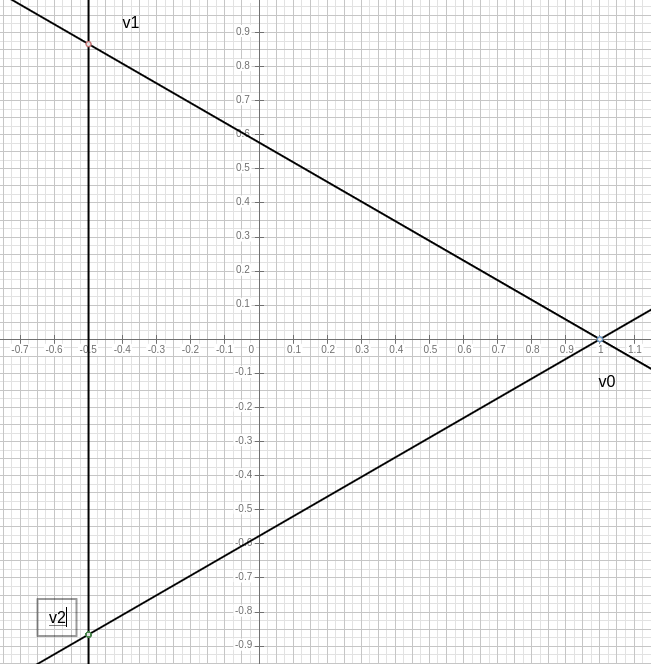
\includegraphics[scale=1,width=0.7\textwidth]{triangulo_n_3.png}
\end{figure}

\begin{figure}[h]
\centering
\caption{Gráfica n=4}
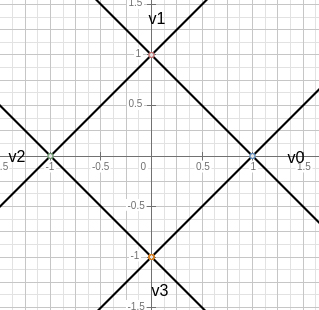
\includegraphics[scale=1,width=0.7\textwidth]{cuadrado_n_4.png}
\end{figure}

Reconocemos $2n$ elementos en $D_n$ que son: \\

Para cada $0\leq k \leq n-1$, sea $R_k$ el giro centrado en el origen y de amplitud $\frac{2k\pi}{n}$. \\

$(R_0=id)$
\begin{gather*}
R_0=id,R_1,R_2,\ldots,R_k \\
R_k:\mathbb{R}^2\rightarrow \mathbb{R}^2 \qquad (x,y)\mapsto (x,y) 
\begin{pmatrix}
cos \frac{2k\pi}{n} & sen\frac{2k\pi}{n} \\
-sen \frac{2k\pi}{n} & cos \frac{2k\pi}{n}
\end{pmatrix}
\end{gather*}

Sean $S_0,S_1,\ldots,S{n-1}$ los n ejes de simetría de $P_n$ que son:

\begin{itemize}
\item Si n es impar, las rectas que unen cada vértice con el origen.

\item Si n es par las rectas que unen cada vértice con el origen y las que unen los puntos medios de cada lado con el origen.
\end{itemize}

Sea $S_k$ la simetría respecto al eje $S_k$. 

\begin{gather*}
0\leq k \leq n-1, \quad S_0,S_1,\ldots,S_{n-1} \\
S_k:\mathbb{R}^2\rightarrow \mathbb{R}^2 \qquad (x,y)\mapsto (x,y)
\begin{pmatrix}
cos\frac{2k\pi}{n} & sen\frac{2k\pi}{n} \\
sen\frac{2k\pi}{n} & -cos\frac{2k\pi}{n}
\end{pmatrix}
\end{gather*}

\textbf{9-3-2021} \\

\textbf{Proposición:} \(D_n=\{R_0,R_1,\ldots,R_{n-1},S_0,S_1,\ldots,S_{n-1}\}\) 
\begin{enumerate}
\item Todo movimiento del plano está totalmente determinado por la imagen de 3 puntos no alineados.

\item Si $T\in D_n$ entonces aplica vértices en vértices:
\begin{equation*}
T|_{\{v_0,\ldots,v_{n-1}\}}:\{v_0,\ldots,v_{n-1}\}\longrightarrow \{v_0,\ldots,v_{n-1}\}
\end{equation*}

\item Si $T\in D_n$, entonces el origen es el único punto fijo.

\item Si $T\in D_n$, entonces $T$ está completamente determinado por $T(v_0)$ y $T(v_1)$.

\item Siempre se cumple que $T(v_0)$ y $T(v_1)$ son vértices adyacentes.

\item Tenemos que
\begin{equation*}
D_n=\{id=R_0,R_1,\ldots,R_{n-1},S_0,\ldots,S_{n-1}\}
\end{equation*}
\end{enumerate}

\textbf{Demsotración:}

\begin{enumerate}[(1)]
\item Todo movimiento del plano está totalmente determinado por la imagen de 3 puntos no alineados.

\item Si \(T\in D_n\) entonces,

\[
\restr{T}{\{v_0,\ldots,v_n\}}:\{v_0,\ldots,v_{n-1}\}\rightarrow \{v_0,\ldots,v_{n-1}\},
\]

define un permutación de vértices.

\begin{itemize}
\item n par y $v_i$ un vértie de $P_n$ y sea $v_j$ el vértice opuesto.

\[
\forall (p,q)\in P_n\times P_n \qquad d(p,q) \leq d(v_i,v_j)
\]

Como T preserva distancias y $T(P_n)=P_n \quad \forall (p,q)\in P_n\times P_n$, entonces $d(p,q)\leq d(T(v_i),T(v_j))=d(v_i,v_j) \Rightarrow T(v_i),\,T(v_j) \in \{v_0,\ldots,v_{n-1}\}$
\item n impar y $v_i$ un vértice de $P_n$ y $v_j$, $v_k$ los vértices del lado opuesto,

\[
\forall (p,q) \in P_n\times P_n \qquad d(p,q) \leq d(v_i,v_j) = d(v_i,v_k)
\]

y entonces $T(v_i),\,T(v_j),\,T(v_k) \in \{v_1,\ldots,v_k\}$

\[
\restr{T}{\{v_1,\ldots,v_n\}}:\{v_0,\ldots,v_{n-1}\}\rightarrow \{v_0,\ldots,v_{n-1}\}
\]

y $\restr{T}{\{v_0,\ldots,v_n\}}$ es inyectiva (T preserva distancias) $\Rightarrow$ $\restr{T}{\{v_0,\ldots,v_{n-1}\}}$ es biyectiva, pues toda isometría es sobreyectiva.
\end{itemize}

\item Si $T \in D_n$ entonces $T(0,0)=(0,0)$ $0=(0,0)$, porque $0$ es el único punto del plano que equidista de todos los vértices.

\item Si $T \in D_n$ entonces $T$ está completamente determinado por $T(v_0)$ y $T(v_1)$. Poque $0,\, v_0,\, v_1$ son tres puntos no alineados y $T(0)=0$ \\

Si $T,T' \in D_n$ tal que 

\[
\left.\begin{array}{c}
T(v_0)=T'(v_0) \\
T(v_1)=T'(v_1)
\end{array}
\right\rbrace 
\Rightarrow T=T'
\]

\item Si $T \in D_n$ entonces $T(v_0)$ y $T(v_1)$ son vértices adyacentes porque los vértices adyacentes de $P_n$ son los de mínima distancia entre los pares de vértices de $P_n$.

\item $D_n=\{R_0 \neq id, R_1, \ldots, R_{n-1}, S_0, \ldots, S_{n-1}\}$ \\

Sea $T\in D_n$ y supongamos $T(v_0)=v_k \quad 0\leq k \leq n-1$.

\begin{itemize}
\item Si $T (v_1)=v_{k+1}$ (entendiendo $v_0$ si $k=n-1$) entonces $T=R_k$, porque $R_k(v_0)=v_k$ y $R_k(v_1)=v_{k+1}$

\item Si $T(v_1)=v_{k-1}$ (entendiendo $v_{n-1}$ si $k=0$) $\Rightarrow^{4)}$ $T=S_k$ porque $S_k(v_0)=v_k$ y $S_k(v_1)=v_{k-1}$
\end{itemize}

\end{enumerate}

Veamos otra forma de trabajar con los grupos $D_n$ (puramente algebraica). \\

\textbf{Ejemplo:} $n=4,\, D_4=\{R_0=id, R_1, R_2, R_3, S_0, S_1, S_2, S_3\}$

\begin{figure}[h]
\centering
\caption{Gráfica ejemplo}
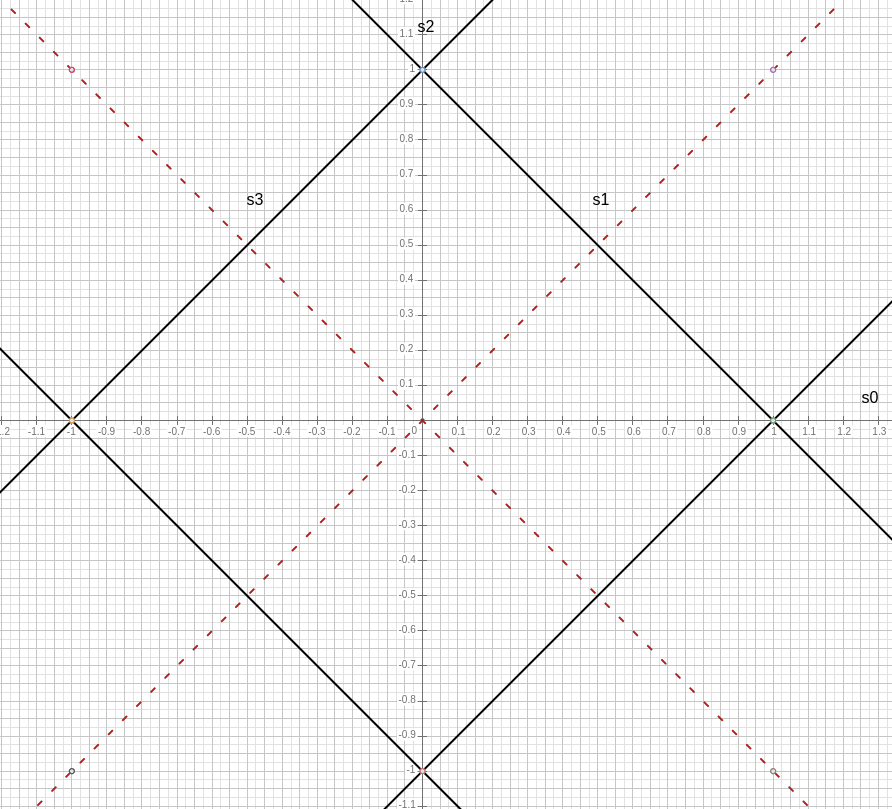
\includegraphics[scale=1,width=0.8\textwidth]{ejemplo_simetrias.png}
\end{figure}

\begin{itemize}
\item $R_0=id$
\item $R_1=$ giro de amplitud $90º$
\item $R_2=$ giro de amplitud $180º$
\item $R_3=$ giro de amplitud $270º$
\item $S_0=$ simetría respecto al eje $s_0$
\item $S_1=$ simetría respecto al eje $s_1$
\item $S_2=$ simetría respecto al eje $s_2$
\item $S_3=$ simetría respecto al eje $s_3$
\item Entonces si $r=R_1$ y $s=S_0$ se tiene,

\[
r^2=R_2,\, r^3=R_3,\, r^4=id
\]
\end{itemize}

$D_4=\{1,r,r^2,r^3,s,rs,r^2s,r^3s\}$ y $r^4=1=s^2$. \\

Se verifica además que $sr=r^3s$. Veámoslo

\[
\left.\begin{array}{c}
sr(v_0)=v_3=S_3(v_0) \\
sr(v_1)=v_2=S_3(v_1)
\end{array}
\right\rbrace \Rightarrow sr=S_3=r^3s
\]

\begin{center}
\begin{tabular}{c|c c c c c c c c}
$\cdot$ & $1$ & $r$ & $r^2$ & $r^3$ & $s$ & $rs$ & $r^2s$ & $r^3s$ \\
\hline
1 & $1$ & $r$ & $r^2$ & $r^3$ & $s$ & $rs$ & $r^2s$ & $r^3s$ \\
$r$ & $r$ & $r^2$ & $r^3$ & 1 & $rs$ & $r^2s$ & $r^3s$ & $s$ \\  
$r^2$ & $r^2$ & $r^3$ & 1 & $r$ & $r^2s$ & $r^3s$ & $s$ & $rs$ \\ 
$r^3$ & $r^3$ & 1 & $r$ & $r^2$ & $r^3s$ & $s$ & $rs$ & $r^2s$ \\ 
$s$ & $s$ & $r^3s$ & $r^2s$ & $rs$ & 1 & $r^3$ & $r^2$ & $r$ \\ 
$rs$ & $rs$ & $s$ & $r^3s$ & $r^2s$ & $r$ & 1 & $r^3$ & $r^2$ \\ 
$r^2s$ & $r^2s$ & $rs$ & $s$ & $r^3s$ & $r^2$ & $r$ & 1 & $r^3$ \\ 
$r^3s$ & $r^3s$ & $r^2s$ & $rs$ & $s$ & $r^3$ & $r^2$ & $r$ & 1 \\ 
\end{tabular}
\end{center}

\begin{gather*}
r^4=1=s^2;\, sr=r^3s \\
sr^2=srr=r^3sr=r^6s=r^2s
\end{gather*}

\textbf{10-3-2021} \\

Sea $n\geq 3$, $D_n=\{id,R_1,R_2,\ldots,R_{n-1},S_0,S_1,\ldots,S_{n-1}\}$. Si llamamos 

\begin{itemize}
\item $r=R_1$, giro centrado en el origen de amplitud $\frac{2\pi}{n}$
\item $s=S_0$, simetría respecto al eje $y=0$
\end{itemize}

Entonces se verifica

\[
\left\lbrace \begin{array}{c}
R_k=r^k \quad 0\leq k \leq n-1 \\
S_k=r^ks \quad 0 \leq k \leq n-1
\end{array} \right.
\]

Además, $r^n=1=s^2$ y $sr=r^{n-1}s$. Es decir,

\[
D_n=\{1,r,r^2,\ldots,r^{n-1},s,rs,r^2s,\ldots,r^{n-1}s\}
\]

y se tiene que 

\[
r^n=1=s^2 \qquad sr=r^{n-1}s \tag{1}
\]

\textbf{Proposición:} Para todo $1 \leq k \leq n-1$ se tiene que

\[
sr^k=r^{n-k}s \tag{2}
\]

y entonces podemos escribir la tabla del grupo $D_n$ haciendo uso únicamente de las identidades $(1)\,y\,(2)$. \\

\textbf{Demostración:} Veamos $(2)$. Hacemos inducción sobre k.

Para $k=1$ se tiene por $(1)$. Supuesto cierto para k,

\begin{gather*}
sr^{k+1}=sr^kr=r^{n-k}sr=^{(1)}r^{n-k}r^{n-1}s= \\
=r^{2n-(k+1)}s=r^nr^{n-(k+1)}s=^{(1)}r^{n-(k+1)}s
\end{gather*}

y se tiene $(2)$.

Nótese que $(2)$ es consecuencia de $(1)$. Notemos además que otra forma de escribir $(2)$ es como sigue

\[
sr^k=r^{-k}s \tag{2'}
\]

porque $r^{-k}=(r^k)^{-1}=r^{n-k}$ ya que $r^kr^{n-k}=r^n=1$. \\

$\hfill\square$

Describir la tabla $D_n$, es decir,

\begin{gather*}
r^ir^j=r^{i+j}=r^{res(i+j;n)} \\
r^ir^js=r^{i+j}s=r^{res(i+j;n)}s \\
r^isr^j=^{(2')}r^ir^{-j}s=r^{i-j}s=r^{res(i-j;n)}s \\
r^isr^js=^{(2')}r^ir^{-j}ss=^{(1)}r^{i-j}=r^{res(i-j;n)} \\
\end{gather*}

Diremos que $D_n$ está generado por r y s y escribiremos

\[
D_n=\left\langle r,s/r^n=1=s^2;\: sr=r^{n-1}s \right\rangle
\]

a las identidades

\[
r^n=1=s^2 \qquad sr=r^{n-1}s
\]

las llamaremos identidades fundamentales.

\begin{gather*}
D_n=\{1,r,\ldots,r^{n-1},s,rs,\ldots,r^{n-1}s\} \\
|D_n|=2n 
\end{gather*}

Puesto que $sr=r^{n-1}s$ y como $n\geq 3$ entonces $sr\neq rs$. Es decir, $D_n$ no es un grupo abeliano para todo n. \\ 

$\hfill\square$

\subsection{Grupo de los cuaternios}

El grupo de los cuaternios, que denotaremos $\mathcal{Q}_2$, es dado por

\[
\mathcal{Q}_2=\left\lbrace \begin{array}{c}
1=
\begin{pmatrix}
1 & 0 \\
0 & 1
\end{pmatrix},\,
-1=
\begin{pmatrix}
-1 & 0 \\
0 & -1
\end{pmatrix}, \,
i=
\begin{pmatrix}
0 & 1 \\
-1 & 0
\end{pmatrix} \\
-i=
\begin{pmatrix}
0 & -1 \\
1 & 0
\end{pmatrix}, \,
j=
\begin{pmatrix}
0 & i \\
i & 0
\end{pmatrix},\,
-j=
\begin{pmatrix}
0 & -i \\
-i & 0
\end{pmatrix}\\
k=
\begin{pmatrix}
i & 0 \\
0 & -i
\end{pmatrix}, \,
-k=
\begin{pmatrix}
-i & 0 \\
0 & i
\end{pmatrix}

\end{array} \right\rbrace
\]

con operación dada por el producto de matrices.

\begin{gather*}
(-1)^{-1}=-1 \\
i^{-1}=-i \Rightarrow (-i)^{-1}=i \\
k^{-1}=-k \Rightarrow (-k)^{-1}=k \\
j^{-1}=-j \Rightarrow (-j)^{-1}=j
\end{gather*}

\textbf{Proposición:} Se verifica,

\begin{enumerate}[a)]
\item $i^2=j^2=k^2=-1 \qquad (-1)^2=1$
\item $i(-1)=-i=(-1)i$
\item $j(-1)=-j=(-1)j$
\item $k(-1)=-k=(-1)k$
\item $ij=k$
\end{enumerate}

\textbf{Demostración:} Se deja como ejercicio. \\

\textbf{Ejercicio:} Prescindiendo de la descripción de los elementos de $\mathcal{Q}_2$ como matrices, y utilizando únicamente las identidades anteriores, a), b), c), d), e), probar que $\mathcal{Q}_2$ se verifica que,

\[
jk=i,\; ki=j,\; ji=-k,\; kj=-1,\; ik=-j
\]

Se puede entonces escribir la tabla de $\mathcal{Q}_2$ prescindiendo de su descripción como matrices. \\

Veamos que $jk=i$. Por ejemplo sabemos que

\begin{gather*}
ij=k\Rightarrow ijk=k^2\Rightarrow ijk=-1 \Rightarrow i^2jk=-1i \Rightarrow \\
\Rightarrow -1jk=-1i \Rightarrow (-1)^2jk=(-1)^2i \Rightarrow jk=i
\end{gather*}

Veamos que $ki=j$. Sabemos que 

\begin{gather*}
jk=i \Rightarrow jki=i^2=-1 \Rightarrow j^2ki=j(-1) \Rightarrow (-1)ki=(-1)j \Rightarrow ki=j
\end{gather*}

Veamos que $ji=-k$. Sabemos que 

\[
ki=j \Rightarrow ki^2=ji \Rightarrow k(-1)=ji \Rightarrow -k=ji
\]

$\mathcal{Q}_2=\{1,-1,i,-i,j,-j,k,-k\}$ verificando las identidades,

\begin{gather*}
(-1)^2=1 \qquad i^2=j^2=k^2=-1 \\
a(-1)=-a=(-1)a \qquad a=i,j,k \\
ij=k
\end{gather*}

\subsection{El grupo de Klein}

\textbf{Definición:} Sean $G$ y $H$ dos grupos. Definimos el producto directo de $G$ y $H$ como el grupo dado por el producto cartesiano

\[
G\times H=\{(x,y)/x \in G,\; y\in H\}
\]

y con producto definido como sigue:

\[
(x,y)(x',y')=(xx',yy')
\]

Es fácil ver que en efecto $G\times H$ es un grupo con la operación anterior, donde el uno es $(1,1)$ y para cada $(x,y)\in G\times H$, su inverso $(x,y)^{-1}=(x^{-1},y^{-1})$. Si $G$ y $H$ son finitos entonces $G\times H$ es finito con 

\[
|G\times H|=|G||H|
\]

Definimos el grupo de Klein, que denotaremos por $K$, como el producto directo de $\mu_2$ con $\mu_2$, donde $\mu_2$ es el grupo de las raíces cuadradas de la unidad.

\begin{gather*}
K:=\mu_2\times \mu_2=\{(1,1),(1,-1),(-1,1),(-1,-1)\} \\
\mu_2=\{x\in \mathbb{C}^* /x^2=1\}=\{1,-1\} \\
|K|=4
\end{gather*}

\textbf{Ejercicio:} Escribir la tabla. \\

\textbf{Definición:} Sean $G$ y $G'$ dos grupos. Un homomorfismo de grupos de $G$ en $G'$ es una aplicación

\[
f:G\rightarrow G'
\]

tal que verifica

\[
f(ab)=f(a)\cdot f(b) \qquad \forall a,b\in G
\]

\begin{itemize}
\item Si $f$ es inyectiva diremos que $f$ es un monomorfismo.
\item Si $f$ es sobreyectiva diremos que $f$ es un epimorfismo.
\item Si $f$ es biyectiva diremos que $f$ es un isomorfismo.
\end{itemize}

\textbf{Ejemplos:}
\begin{enumerate}[1)]
\item Para todo grupo $G$, $1_G:G\rightarrow G$ es un isomorfismo

\item $n\geq 2$, $K$ cuerpo

\[
det:GL_n(K)\rightarrow K^*
\]

es un homomorfismo (con el producto).

\item $\mathbb{R}\xrightarrow{f}\mathbb{R}^* \quad f(x)=e^x$ (con la suma $f(x+y)=f(x)\cdot f(y)$)

\item Para todo $n\geq 2$

\begin{gather*}
p:\mathbb{Z}\rightarrow \mathbb{Z}_n \\
p(k)=res(k;n)
\end{gather*}
\end{enumerate}

\textbf{Ejercicio:} Sea $f:G\rightarrow G'$ un homomorfismo de grupos. Entonces

\begin{enumerate}[(i)]
\item $f(1)=1$
\item $f(a^{-1})=f(a)^{-1} \qquad \forall a\in G$
\end{enumerate}

\textbf{Proposición:} Sean $f:G\rightarrow G'$ y $g:G'\rightarrow G''$ dos aplicaciones. Entonces

\begin{enumerate}[(i)]
\item Si f y g son homomorfismos $\Rightarrow$ $g\circ f$ es un homomorfismo.

\item Si f y g son monomorfismos (respectivamente, epimorfismos, isomorfismos) $\Rightarrow$ $g\circ f$ (respectivamente, epimorfismo, isomorfismo).
\end{enumerate}

\textbf{Demostración:} Se deja como ejercicio. \\

\textbf{Proposición:} Sea $f:G\rightarrow G'$ un homomorfismo. Entonces 

\begin{gather*}
f~es~isomorfismo \Leftrightarrow \exists g:G'\rightarrow G~tal~que \\
f \circ g=id_{G'}~y~g\circ f=id_{G}
\end{gather*}

Además, en tal caso g es única y se denota por $f^{-1}:G'\rightarrow G$. \\

\textbf{Dem:} $\Leftarrow)$ Obvio. \\

$\Rightarrow)$ $f:G\rightarrow G'$ isomorfismo. Entonces f es una aplicación biyectiva y por tanto $\exists g:G'\rightarrow G$ tal que

\[
f \circ g=id_{G'} \quad y \quad g\circ f=id_{G}
\]

Veremos que $g:G'\rightarrow G$ es un homomorfismo de grupos:

\begin{gather*}
\forall x',y'\in G \qquad g(x'y')=^{?}g(x')g(y') \\
g(x'y')\in G \qquad g(x')g(y')\in G \\
f(g(x'y')=(f\circ g)(x'y')=x'y' \\
f(g(x')g(y'))=f(g(x'))f(g(y'))=(f\circ g)(x')(f\circ g)(y')=x'y' \\
f(g(x'y'))=f(g(x')g(y')) \Rightarrow^{f\> inyectiva} g(x'y')=g(x')g(y')
\end{gather*}

\textbf{Corolario:} En la clase de todos los grupos, la relación binaria ``ser~isomorfos'' es una relación de equivalencia. \\

\textbf{Demostración:} Dados dos grupos $G$ y $G'$ diremos que $G$ es isomorfo a $G'$ si existe un isomorfismo $f:G\rightarrow G'$ y lo denotaremos por $G\cong G'$. \\

``Ser isomorfo'' es una relación binaria en la clase de todos los grupos. Puesto qeu $1_G:G\rightarrow G$ es un isomorfismo $\Rightarrow$ $G\cong G \quad \forall G$ (propiedad reflexiva). \\

Si $G\cong G'$ es porque $\exists f:G\rightarrow G'$ isomorfismo $\Rightarrow$ $f^{-1}:G'\rightarrow G$ es un isomorfismo $\Rightarrow$ $G'\cong G$ (propiedad simétrica). \\

Si

\[
\left.\begin{array}{c}
G \cong G' \\
G'\cong G''
\end{array} \right\rbrace
\left. \begin{array}{c}
\exists f:G\rightarrow G'~isomorfismo \\
\exists g:G'\rightarrow G''~isomorfismo
\end{array} \right\rbrace
\Rightarrow
\]

$g\circ f:G\rightarrow G''$ es un isomorfismo $\Rightarrow G\cong G''$ (propiedad transitiva). \\

$\hfill\square$

Uno de los objetivos de la teoría de grupos finitos es su clasificación. Es decir, obtener un listado de todos los grupos finitos no isomorfos entre sí. \\

\textbf{15-3-2021} \\

\textbf{Teorema:} Todos los grupos de orden 2 son isomorfos entre sí. Es decir, hay sólo una calse de equivalencia que la representaremos por el grupo $\mu_2=\{1,-1\}$ \\

\textbf{Demostración:} $G=\{1,a\}, \quad H=\{1,b\}$ \\

Definimos,

\begin{gather*}
f:G\rightarrow H \\
f(1)=1 \\
f(a)=b
\end{gather*}

$f$ es un homomorfismo de grupos y entronces isomorfismo 

\begin{equation*}
f(xy)=f(x)f(y) \qquad \forall x,y \in G
\end{equation*}

Es obvio que se tiene si $x=1$ ó $y=1$. Si $x=y=a$, entonces $xy=a^2=1$ \\

\begin{tabular}{c | c c}
$\cdot$ & 1 & a \\
\hline
1 & 1 & a \\
a & a & 1
\end{tabular} \\

\begin{gather*}
(a^2\neq a \, pues\, a^2=a \Rightarrow a=1) \\
\left. \begin{array}{c}
f(xy)=f(a^2)=f(1)=1 \\
f(x)\cdot f(y)=f(a)\cdot f(a)=b^2=1 \, (analogo \, al \, caso \, de \, a)
\end{array} \right\rbrace
\Rightarrow f(a^2)=f(a)\cdot f(a)
\end{gather*}

\textbf{Ejercicios:} 

\begin{itemize}
\item \textbf{Ejercicio 5) Rel 1:} No cumple la propiedad asociativa
\item \textbf{Ejercicio 6) Rel 1:} $y,x\in G$, se tiene como hipótesis $x^2=1,\, y^2=1$. \\

\begin{gather*}
(xy)^2=xyxy=1 \Rightarrow x^2yxy^2=xy
\end{gather*}

lo que implica que G es un grupo abeliano.

\item \textbf{Ejercicio 7) Rel 1:}
\begin{itemize}
\item $1)\Rightarrow 2)$ obvio $(xy)^2=xyxy=xy^2x=x^2y^2$.
\item $2)\Rightarrow 3)$
	\begin{gather*}
	(x^{-1}y^{-1})^2=x^{-1}y^{-1}x^{-1}y^{-1}=^{(2)} \\
=^{(2)}x^{-1}x^{-1}y^{-1}y^{-1} \Rightarrow y^{-1}x^{-1}=(xy)^{-1}=x^{-1}y^{-1}
	\end{gather*}
\item $3)\Rightarrow 1)$ Puesto que

\begin{equation*}
(xy)^{-1}=x^{-1}y^{-1} \Rightarrow xyx^{-1}y^{-1}=1 \Rightarrow xy=yx
\end{equation*}
\end{itemize}

\item \textbf{Ejercicio 9) Rel 1:} $G=\{f:\mathbb{R}\rightarrow\mathbb{R}/f(x)=ax+b,\,a,\,b\in \mathbb{R}\, a\neq 0\}$ 

\begin{gather*}
\mathbb{R}\xrightarrow{f} \mathbb{R} \xrightarrow{g} \mathbb{R} \\
f(x)=ax+b, \quad g(x)=a'x+b \quad a,a' \neq 0 \\
(g\circ f)(x)=g(ax+b)=a'(ax+b)+b'=a'ax+a'b+b' \quad a'a\neq 0 \\
\Rightarrow g\circ f \in G
\end{gather*}

\textbf{Propiedad Asociativo}
\begin{equation*}
1_R \in G \quad 1_R(x)=x=1x+0 \quad a=1, \quad b=0
\end{equation*}

\textbf{Comprobar inversos:} $f: \mathbb{R} \rightarrow \mathbb{R} \quad f(x)=ax+b$
\begin{gather*}
f^{-1}:\mathbb{R}\rightarrow \mathbb{R}\quad es \quad f^{-1}(x)=\frac{1}{a}x-\frac{b}{a} \\
f\circ f^{-1}(x)=f(\frac{1}{a}x-\frac{b}{a})=x
\end{gather*}

\item \textbf{Ejercicio 10) Rel 1:} $GL_2(\mathbb{Z}_2)=\left\lbrace
\begin{pmatrix}
a & b \\
c & d
\end{pmatrix}
\in \mathcal{M}_2(\mathbb{Z}_2) /ad=bc=1\right\rbrace$ 
\begin{enumerate}[(1)]
\item 
\begin{equation*}
GL_2(\mathcal{M}_2)=\left\lbrace
\begin{pmatrix}
1 & 0 \\
0 & 1
\end{pmatrix},
\begin{pmatrix}
1 & 0 \\
1 & 1
\end{pmatrix},
\begin{pmatrix}
1 & 1 \\
1 & 0
\end{pmatrix},
\begin{pmatrix}
1 & 1 \\
0 & 1
\end{pmatrix},
\begin{pmatrix}
0 & 1 \\
1 & 1
\end{pmatrix},
\begin{pmatrix}
0 & 1 \\
1 & 0
\end{pmatrix} \right\rbrace
\end{equation*}

$|GL_2(\mathbb{Z}_2)|=6$

\item $GL_2(\mathbb{Z}_2)=\{1,\alpha,\alpha^2,\beta,\alpha\beta,\alpha^2\beta\}$.

\item Escribir la tabla de $GL_2(\mathbb{Z}_2)$, usando la representación de (2). Comprobar que

\begin{equation*}
\left. \begin{array}{c}
\alpha^3=1=\beta^2 \\
\beta\alpha=\alpha^2\beta
\end{array} \right\rbrace
\end{equation*}

Entonces escribir la tabla sin necesidad de recurrir a su descripción como matrices. \\
\end{enumerate}

\item \textbf{16-3-2021}

\item \textbf{Ejercicio 21) Rel 1:} 

\begin{enumerate}[1)]
\item
\begin{gather*}
1 \mapsto 1 \quad i\mapsto 2 \\
-1 \mapsto 4 \quad -i\mapsto 3 \\
\mu_4=\{1,-1,i,-i\}\xrightarrow{x}\mathbb{Z}_5^x=\{1,2,3,4\}
\end{gather*}

\item Otro isomorfismo

$g:\mu_4 \rightarrow \mathbb{Z}_5^x $isomorfismo de grupos

$g(1)=1$ pues g ha de ser homomorfismo 

\begin{equation*}
g(-1)=4 \quad g(i)=3 \quad g(-i)=2 
\end{equation*}

Comprobar que $g:\mu_4\rightarrow \mathbb{Z}_5^x$ es homomorfismo de grupos y isomorfismocon $g \neq f$.
\end{enumerate}

\item \textbf{Ejercicio 26) Rel 1:} 

\begin{enumerate}[1)]
\item $\mathbb{R}^*$ no es isomorfo a $\mathbb{C}^*$.

\begin{equation*}
\exists f:\mathbb{C}^*\rightarrow \mathbb{R}^* \quad isomorfismo
\end{equation*}

Sea $f(i)=a\in \mathbb{R}^*$.

\begin{gather*}
1=f(1)=f(i^4)=f(i)^4=a^4 \Rightarrow \xcancel{a = 1}\quad o\quad =-1´
\end{gather*}

$a=1$ no puede ser pues $i\neq 1$ y por tanto $f(i)\neq f(1)=1$. Luego de aquí se deduce
\

\begin{gather*}
f(i)=-1 \Rightarrow f(i)\cdot f(i)=(-1)(-1)=1=f(i^2)=f(-1)
\end{gather*}

luego se llega a contradicción con que f es inyectiva

\item $\mathbb{Z}$ y $\mathbb{Q}$ isomorfismo. Sea $g(1)=\frac{a}{b}$ entonces para $n \in \mathbb{Z}$ se tendrá que

\begin{gather*}
n>0 \quad g(n)=g(1+\ldots+1)=g(1)+\ldots+g(1)=n\cdot \frac{a}{b} \\
g(-n)=-g(n)=-n\frac{a}{b}, \qquad g(0)=0
\end{gather*}

Elegimos $p \in \mathbb{Z}$ primo tal que $p \nmid b$ y consideramos $\frac{1}{p} \in \mathbb{Q}$. Como g es sobreyectiva, $\exists n \in \mathbb{Z}$ tal que 

\begin{gather*}
g(n)=n\frac{a}{b}=\frac{1}{p}\Rightarrow p\cdot n\cdot a=b \Rightarrow p\mid b
\end{gather*}

Lo cual es una contradicción.

\end{enumerate}
\end{itemize}

\textbf{Definición:} Sea K un cuerpo, se define su característica como el menor entero positivo tal que $n\cdot 1=0$. Si no existe ningún entero n positivo verificando que $n\cdot 1=0$, se dice que K tiene característica 0

\begin{gather*}
Car(\mathbb{R})=0=Car(\mathbb{Q})=Car(\mathbb{C}) \\
Car(\mathbb{Z}_p)=p\quad p 	\quad primo
\end{gather*}

\textbf{Ejercicio 28) Rel 1:} Supongamos que $\exists f:K^*\rightarrow K$ isomorfismo tal que 

\begin{gather*}
\left\lbrace \begin{array}{c}
f(xy)=f(x)+f(y) \quad \forall x,y\in K^* \\
f(1)=0
\end{array} \right. \\
0=f(1)=f((-1)(-1))=f(-1)+f(-1) \\
\left.\begin{array}{c}
2\cdot f(-1)=0 \\
Si \: Car(K)\neq 2
\end{array} \right\rbrace
\Rightarrow f(-1)=0 \\
\Rightarrow f(-1)=f(1)
\end{gather*}

Lo cual es contradicción con que f sea inyectiva. Por otro lado supongamos que $Car(K)=2$. Consideremos $f^{-1}:K\rightarrow K^*$ es también un isomorfismo

\begin{gather*}
\left\lbrace \begin{array}{c}
f^{-1}(x+y)=f^{-1}(x)\cdot f^{-1}(y) \quad \forall x,y \in K \\
f^{-1}(0)=1
\end{array} \right.
\end{gather*}

Sea $a\in K^*$ arbitrario. Como $f^{-1}$ es sobreyectiva $\Rightarrow \exists b \in K$ tal que

\begin{gather*}
f^{-1}(b)=a \\
a^2=f^{-1}(b)f^{-1}(b)=f^{-1}(b+b)= f^{-1}(2b)=^{Car(K)=2}f^{-1}(0)=1 \\
\Rightarrow a^2=1 \Rightarrow a=1
\end{gather*}

Por tanto $K^*=\{1\}$ con lo que $K=\{0,1\}$ y por tanto no son conjuntos biyectivos.

\begin{gather*}
\left\lbrace \begin{array}{c}
a^2=1 \Rightarrow a\>es\>raiz\>de\> x^2-1,\> que\> son\> 1,-1 \\
Como\> Carac(K)=2 \qquad 2\cdot 1=1+1=0 \Rightarrow 1=-1
\end{array} \right.
\end{gather*}

\textbf{17-3-2021} \\

\section{Tema 3. Subgrupos. Generadores. Retículos}

\textbf{Definición:} Sea G un grupo. Un subgrupo de G es un subconjunto $H\subseteq G$, $H \neq \emptyset$ que verifica

\begin{enumerate}[(1)]
\item Para cualesquiera $x,y\in H, \quad xy\in H$

\item $1 \in H$

\item $\forall x  \in H,\quad x^{-1}\in H$
\end{enumerate}

Por tanto H con el producto en G tiene también estructura de grupo. Cuando H sea subgrupo de G, lo escribiremos de la forma: $H \leq G$. \\

\textbf{Ejemplos:}

\begin{enumerate}[1)]
\item Para todo grupo G, el conjunto $\{1\}$ y G son subgrupos de G. A estos los llamaremos subgrupos impropios de G. El subgrupo $\{1\}$ se le llama subgrupo trivial de G. Los demás subgrupos, si los hay, se llaman subgrupos propios $\Rightarrow \{1\} \leq H \leq G \: con \: \{1\}\neq H\neq G$

\item $\mathbb{Q}^*\leq \mathbb{R}^*\leq \mathbb{C}^*$

\item $\forall n \geq 1 \quad \mu_n\leq \mathbb{C}^*$

\item Si $m,n \geq 1$ y $m \mid n \Rightarrow \mu_m \leq \mu_n$
\end{enumerate}

\textbf{Proposición:} Sea G un grupo y $H \subset G,\: H\neq \emptyset$, entonces H es un subgrupo de G $\Leftrightarrow$ para cualesquiera $x,y\in H, \: xy^{-1}\in H$ \\

\textbf{Demostración:} $\Rightarrow)$ Es clara. \\

$\Leftarrow)$ Como $H \neq \emptyset$, elegimos $x \in H$. Entonces tomando $y=x$, por hipótesis, $xy^{-1}=xx^{-1}=1\in H$ y por tanto se tiene (2) \\

Sea $x\in H$ y consideramos $1 \in H$. Entonces, por hipótesis, $1\cdot x^{-1}=x^{-1}\in H$. Se tiene así (3). \\

Sean $x,y\in H\Rightarrow xy^{-1}\in H\Rightarrow^{hip.} x(y^{-1})^{-1}=xy\in H$ y se tiene (1).

$\hfill\square$ \\

\textbf{Proposición:} Sea G un grupo finito y $H \subset G$, $H \neq \emptyset$. Entonces H es un subgrupo de G $\Leftrightarrow$ Para cualesquiera $x,y\in H,\: xy\in H$. \\

\textbf{Demostración:} $\Rightarrow)$ Es obvio, por definición de subgrupo. \\

$\Leftarrow)$ Por hipótesis verifica (1). \\

Sea $x \in H$. Consideramos $x, x^2, x^3, \ldots, x^n, \ldots$ todos son elementos de H, por hipótesis. 

Puesto que G es finito, podemos asegurar que $\exists n,m,\: n\neq m$, tal que $x^n=x^m$. Sea $n>m$ y entonces $x^n\cdot x^{-m}=x^m\cdot x^{-m}$, es decir $x^{n-m}=1$. Además, $n-m>0$ y entonces $1=x^{n-m}\in H$. Se tiene (2) \\

Si $x^{n-m}=1\Rightarrow x^{-1}=x^{n-m-1}$, pero $n-m>0 \Rightarrow n-m-1\geq 0$ y así $x^{-1}=x^{n-m-1} \in H$ y se tiene (3).

$\hfill\square$ \\

\textbf{Ejemplo:} 
\begin{enumerate}[1)]
\item Sea $n \geq 3$. En $D_n=\{1,r,\ldots,r^{n-1},s,rs,\ldots,r^{n-1}s\}$. Además se verifican las identidades $r^2=1=s^2, \: sr=r^{n-1}s$.

\begin{equation*}
C=\{1,r,\ldots,r^{n-1}\}\leq D_n
\end{equation*}
pues $r^ir^j=r^{Res(i+j;n)}\in C$. \\

Para cada $0\leq k \leq n-1$, $H_k=\{1,r^ks\}\leq D_n$ \\

\begin{tabular}{c | c c}
$\cdot$ & 1 & $r^ks$ \\
\hline 
1 & 1 & $r^ks$ \\
$r^ks$ & $r^ks$ & 1
\end{tabular} \\

El conjunto $X=\{1,s,rs,\ldots,r^ks\}$ no es un subgrupo de $D_n$ porque la operación no es interna en $X$

\begin{equation*}
s(rs)=srs=r^{n-1}ss=r^{n-1}
\end{equation*}

\item En $S_4$, $K=\{id, \alpha_1=
\begin{pmatrix}
1 & 2
\end{pmatrix}
\begin{pmatrix}
3 & 4
\end{pmatrix},\, 
\alpha_2=
\begin{pmatrix}
1 & 3
\end{pmatrix}
\begin{pmatrix}
2 & 4
\end{pmatrix},\, 
\alpha_3=
\begin{pmatrix}
1 & 4
\end{pmatrix}
\begin{pmatrix}
2 & 3
\end{pmatrix}\}$
\end{enumerate}

Es un subgrupo de $S_4$ \\

\begin{tabular}{c | c c c c}
$\cdot$ & 1 & $\alpha_1$ & $\alpha_2$ & $\alpha_3$ \\
\hline
1 & 1 & $\alpha_1$ & $\alpha_2$ & $\alpha_3$ \\ 
$\alpha_1$ & $\alpha_1$ & 1 & $\alpha_3$ & $\alpha_2$ \\
$\alpha_2$ & $\alpha_2$ & $\alpha_3$ & 1 & $\alpha_1$ \\
$\alpha_3$ & $\alpha_3$ & $\alpha_2$ & $\alpha_1$ & 1
\end{tabular} \\ 

se llama el grupo de Klein de $S_4$. \\

\textbf{Proposición:} Sea $f: G \rightarrow G'$ un homomorfismo de grupos. Entonces

\begin{enumerate}[(i)]
\item $H \leq G \Rightarrow f_*(H)\leq G' \qquad$ ($f_*(H):=\{f(x)/x\in H\}$)

\item Si $H'\leq G' \Rightarrow f^*(H')\leq G \qquad$ ($f^*(H'):=\{x\in G:f(x)\in H'\}\subset G$)

\item $Ker(f)=\{x \in G/f(x)=1\} \leq G$ 

$Img(f)=\{f(x)/x\in G\}\leq G'$

\item f es monomorfismo $\Leftrightarrow Ker(f)=\{1\}$ 

f es epimorfismo $\Leftrightarrow Img(f)=G'$
\end{enumerate}

\textbf{Demostración:}
\begin{enumerate}[\bfseries (i)]
\item $H \leq G \Rightarrow f_*(H)\subset G'$ y $f_*(H)\neq \emptyset$ pues $H\neq \emptyset$. Sean $x',y'\in f_*(H) \Rightarrow~\exists x,y\in~H$ tal que $x'=f(x)$, $y'=f(y)$.

\begin{gather*}
x'(y')^{-1}=f(x)\cdot f(y)^{-1}=f(x)f(y^{-1})=f(xy^{-1})\in f_*(H)
\end{gather*}

Si $x,y\in H \Rightarrow xy^{-1} \in H$.

\item $H'\leq G'$ entonces $f^*(H')\subset G$ y, como $f(1)=1\in H' \Rightarrow 1\in f^*(H')$, entonces $f^*(H')\neq \emptyset$

Sean $x,y\in f^*(H')\Rightarrow f(x),f(y)\in H' \Rightarrow f(x)f(y)^{-1}\in H'=f(xy)^{-1} \Rightarrow xy^{-1}\in f(H')$ 

\item $Ker(f)=f^*(\{1\})\leq G$

$Img(f)=f_*(G)\leq G'$

\item Ejercicio
\end{enumerate}

$\hfill\square$ \\

\subsection{Grupos Alternados:}
Sea $n\geq 2$. Si $(x_1x_2\ldots x_r)$ es un r-ciclo en $S_n$, entonces 

\begin{equation*}
(x_1x_2\ldots x_r)=(x_1x_2)(x_2x_3)\ldots(x_{r-1}x_r)
\end{equation*}

Todo ciclo se expresa como producto de transposiciones

\begin{gather*}
(1\:2\:3\:4)=(1\:2)(2\:3)(3\:4)= \\
=(1\:3)(1\:2)(3\:4)=(2\:4)(1\:3)(2\:4)(1\:2)(3\:4)
\end{gather*}

Como consecuencia todo elemento de $S_n$ se expresa como producto de transposiciones. Por ejemplo, podemos demostrar la identidad como $[id=(1\:2)(1\:2)]$. Dicha expresión no es única. \\

\textbf{Teorema:} Sea $n\geq 2$ y $\alpha \in S_n$. Supongamos que $\alpha=\tau_1\tau_2\ldots\tau_s$, $\tau_i$ es una transposición $\forall i$.

\begin{equation*}
\alpha=\tau_1'\tau_2'\ldots\tau_r' \qquad \tau_j'\:transposicion\: \forall j
\end{equation*}

Entonces $s\equiv r \mod{(2)}$. \\

\textbf{Demostración:} Lo probamos primero para $\alpha=id$. Como $\alpha=(1\:2)(1\:2)$, entonces basta demostrar que si 

\begin{equation*}
id=\tau_1\tau_2\ldots\tau_r\Rightarrow r\equiv 0\mod{(2)}
\end{equation*}

, donde $\tau_i$ es una transposición $\forall i$. Hacemos inducción en r. El primer caso $r=2$ y es claro que se verifica. Supongamos $r>2$, y el resultado cierto para cualquier expresión $id$ como producto de menos de r transposiciones.

Elegimos $m\in \{1,2,\ldots,n\}$ que aparezca en alguna de las transposiciones, $\tau_s'$. Sea $\tau_j$ la 1ª en la que aparece m. Será $\tau_j=(m\:x)$. Aseguramos que $j<r$, porque si $j=r$

\begin{equation*}
id(x)=\tau_1\tau_2\ldots\tau_r(x)=\tau_1\tau_2\ldots\tau_{r-1}(m)=m\neq x
\end{equation*}

Así $j<r$ y podemos considerar $\tau_{j+1}$

\begin{enumerate}
\item $\tau_j\tau_{j+1}=(m\:x)(m\:x)=id$
\item $\tau_j\tau_{j+1}=(m\:x)(m\:y)=(x\:y)(m\:x)$
\item $\tau_j\tau_{j+1}=(m\:x)(y\:z)=(y\:z)(m\:x)$
\item $\tau_j\tau_{j+1}=(m\:x)(x\:y)=(x\:y)(m\:y)$
\end{enumerate}

Sustituyendo en la expresión de $id(x)$ obtenemos en el 1º caso que 

\begin{gather*}
id=\tau_1\ldots\tau_{j-1}\tau_{j+2}\ldots\tau_r \Rightarrow r-2 \equiv 0 \mod{(2)} \Rightarrow \\
\Rightarrow r \equiv 0 \mod{(2)}\:y\:quedaria\:demostrado
\end{gather*}

En los casos 2º, 3º y 4º obtenemos

\begin{equation*}
id=\tau_1\ldots\tau_{j-1}\tau_j'\tau_{j+1}'\tau_{j+2}\ldots\tau_r
\end{equation*}

donde la aparición de m se traslada al lugar j+1.

Repitiendo el proceso, las veces que haga falta, y teniendo en cuenta que no puede ser que m aparezca por primera vez en la última transposición, en algún momento nos encontraremos en la situación 1ª. Es decir, en un número finito de pasos, llegamos a que 

\begin{equation*}
id=\tau_1'\ldots\tau_{r-2}'
\end{equation*}

con $\tau_i'$ transposiciones $\forall i$. Por hipótesis de inducción, $r-2\equiv 0 \mod{(2)} \Rightarrow r \equiv 0 \mod{(2)}$

Sea $\alpha=\tau_1\tau_2\ldots\tau_r\quad y \quad\alpha=\tau_1'\tau_2'\ldots\tau_s' \qquad \tau_i,\tau_j'$ son transposiciones $\forall i \forall j$.

\begin{gather*}
\tau_1\tau_2\ldots\tau_r=\tau_1'\tau_2'\ldots\tau_s'\Rightarrow id=\tau_1\tau_2\ldots\tau_r(\tau_1'\tau_2'\ldots\tau_s')^{-1}= \\
=\tau_1\tau_2\ldots\tau_r\tau_s'^{-1}\ldots\tau_2'^{-1}\tau_1'^{-1}=\tau_1\tau_2\ldots\tau_r\tau_s'\ldots\tau_2'\tau_1'
\end{gather*}

Entonces $r+s\equiv 0 \mod{(2)}\Leftrightarrow r\equiv s \mod{(2)}$

$\hfill\square$ \\

\textbf{Definición:} Sea $n\geq 2$. Una permutación $\alpha \in S_n$ diremos que es par (respectivamente, impar) si se expresa como producto de un número par de transposiciones (respectivamente, un número impar). \\

\textbf{Ejemplo:} $id\in S_n$ es permutación par. Cualquier transposición es impar.

\begin{equation*}
(x_1x_2x_3)=(x_1x_2)(x_2x_3) \: es \: par
\end{equation*}

Como $(x_1x_2\ldots x_r)=(x_1x_2)(x_2x_3)\ldots(x_{r-1}x_r)$.

$(x_1\ldots x_r)$ es par (respectivamente, impar) $\Leftrightarrow$ r es impar (respectivamente, par). \\

\textbf{Definición:} Sea $n\geq 2$ y $\alpha \in S_n$. Definimos la signatura de $\alpha$, que denotamos por $S(\alpha)$, como

\begin{equation*}
s(\alpha)=\left\lbrace \begin{array}{c}
1 \qquad si\:\alpha\:es\:par \\
-1 \qquad si\:\alpha\:es\:impar
\end{array} \right.
\end{equation*}

Se tiene $s:S_n\rightarrow \mu_2=\{1,-1\}$ es un homomorfismo de grupos. \\

\textbf{Demostración:} Sea $\alpha,\beta \in S_n$ \\

Sea $\alpha=\tau_1\tau_2\ldots\tau_r$ una expresión de $\alpha$ como producto de transposiciones, y $\beta=\tau_1'\tau_2'\ldots\tau_s'$ una expresión de $\beta$ como producto de transposiciones. \\

Entonces $s(\alpha)=(-1)^r$ y $s(\beta)=(-1)^s$ 

\begin{gather*}
\alpha\beta=\tau_1\tau_2\ldots\tau_r\tau_1'\tau_2'\ldots\tau_s'\Rightarrow s(\alpha\beta)=(-1)^{r+s} \\
s(\alpha\beta)=(-1)^{r+s}=(-1)^r(-1)^s=s(\alpha)s(\beta)
\end{gather*}

$\hfill\square$ \\

\textbf{Definición:} Sea $n\geq 2$. Definimos el n-ésimo grupo alternado, que denotaremos por $A_n$, como

\begin{equation*}
A_n:=\{\alpha\in S_n/s(\alpha)=1\}
\end{equation*}

que es un subgrupo de $S_n$, pues $A_n=Ker(s)$\\

\textbf{Ejemplo:} $n=2$, $S_2=\{id,(1\:2)\}$ y $A_2=\{id\}$ \\

n=3
\begin{equation*}
\left\lbrace \begin{array}{c}
S_3=\{id, (1\:2\:3),(1\:3\:2),(1\:2),(1\:3),(2\:3)\} \\
A_3=\{id,(1\:2\:3),(1\:3\:2)\}
\end{array} \right.
\end{equation*}

n=4
\begin{equation*}
\left\lbrace \begin{array}{c}
A_4=\{id, (1\:2\:3),(1\:3\:2),(1\:2\:4),(1\:4\:2),(1\:3\:4),(1\:4\:3), \\
(2\:3\:4),(2\:4\:3),(1\:2)(3\:4),(1\:3)(2\:4),(1\:4)(2\:3)\} \\
\end{array} \right.
\end{equation*}

\textbf{Proposición:} $\forall n \geq 2$ se verifica

\begin{equation*}
\left | A_n | \right. = \frac{n!}{2}
\end{equation*} 

\textbf{22-3-2021} \\

\textbf{Demostración:} Consideramos $z=(1\,2) \in S_n$ y sea

\begin{equation*}
(1\,2)A_n=\{(1\,2)\alpha / \alpha \in A_n\}
\end{equation*}

Es claro que todos los elementos de $(1\,2)A_n$ son permutaciones impares. Si $\sigma \in S_n$ es una permutación impar entonces $\sigma \in (1\,2)A_n$ porque

\begin{equation*}
\sigma=(1\,2)(1\,2)\sigma
\end{equation*}

pues sigma es impar $\Rightarrow (1\,2)\sigma \in A_n \Rightarrow (s((1\,2)\sigma))=s(1\,2)s(\sigma)=(-1)(-1)=~1$. \\

Consecuentemente el conjunto $(1\,2)A_n$ es el conjunto de las permutaciones impares de $S_n$. Así tenemos

\begin{equation*}
\left. \begin{array}{c}
A_n\cup (1\,2)A_n=S_n \\
A_n\cap (1\,2)A_n=\emptyset
\end{array} \right\rbrace
\Rightarrow |S_n|=|A_n|+|(1\,2)A_n|
\end{equation*}

Por otro lado la aplicación
\begin{gather*}
\lambda:A_n \rightarrow (1\,2)A_n \\
\lambda(\alpha):=(1\,2)\alpha
\end{gather*}

es biyectiva y entonces $|A_n|=|(1\,2)A_n|$. Tenemos que 
\begin{equation*}
|S_n|=|A_n|+|(1\,2)A_n|=2|A_n|\Rightarrow |A_n|=\frac{|S_n|}{2}
\end{equation*}

$\hfill\square$ \\

Para un grupo $G$, denotaremos $Sub(G)$ a la familia de todos los subgrupos de $G$.

\begin{equation*}
Sub(G)=\{H\subseteq G/H\:es\:un\:subgrupo\:de\:G\}
\end{equation*}

Se tiene que $Sub(G)$ es un conjunto ordenado por la inclusión. $Sub(G)$ es un retículo. \\

\textbf{Definición:} Un conjunto $(X,\leq)$ ordenado se dice un retículo si $\forall x,y\in X$, existe $Inf\{x,y\}$ y existe el $Sup\{x,y\}$. \\

\textbf{Proposición:} Sea G un grupo y $\{H_i\}_{i \in I}$ una familia de subgrupos de G. Entonces
\begin{equation*}
\cap_{i\in I}H_i
\end{equation*}

es también un subgrupo de G. \\

\textbf{Demostración:} Ejercicio. \\

\textbf{Corolario:} $Sub(G)$ es un retículo. \\

\textbf{Demostración:} Sean $H_1,\,H_2\in Sub(G)$

\begin{equation*}
Inf\{H_1,H_2\}=H_1\cap H_2
\end{equation*}

Si $K \subseteq H_1$ y $K \leq H_2 \Rightarrow K \leq H_1 \cap H_2$

\begin{itemize}
\item $Sup\{H_1,H_2\}=\cap_{k \in Sub(G),\:H_i\leq K\: i=1,2} K \in Sub(G)$
\end{itemize}

$\hfill\square$ \\

\textbf{Notación:} Denotaremos el supremo $Sup\{H_1,H_2\}=H_1\lor H_2$. (La unión de subgrupos no es en general un subgrupo 

\begin{equation*}
G=D_3=\left\langle \begin{array}{c}
r,s/r^3=1=s^2,\: sr=r^2s
\end{array} \right\rangle 
=\{1,r,r^2,s,rs,r^2s\}
\end{equation*}
$H_1=\{1,s\},\qquad H_2=\{1,rs\}$ 

\begin{equation*}
H_1\cup H_2=\{1,s,rs\}
\end{equation*}

no es un subgrupo de $D_3$. ($(rs)\cdot s=rs^2=r \notin H_1\cup H_2$)). \\

¿Quién es $H_1\lor H_2$? $r,rs\in H_1\lor H_2 \Rightarrow (rs)s=rs^2=r\in H_1\lor H_2$. 

\begin{equation*}
H_i\subseteq H_1\lor H_2 \qquad i=1,2
\end{equation*}

Si $r \in H_1\lor H_2$, $s\in H_1\lor H_2 \Rightarrow G \leq H_1\lor H_2 \Rightarrow H_1\lor H_2 =G$. \\

\textbf{Notación:} Sea G un grupo y $X$, $Y$ subconjuntos no vacíos de G. Denotaremos $XY$ al conjunto

\begin{equation*}
XY:=\{xy/x\in X, y \in Y\}
\end{equation*}

si $X=\{a\}$ escribiremos $aY=\{ay/y\in Y\}$

si $Y=\{b\}$ escribiremos $Xb=\{xb/x\in X\}$. \\

\textbf{Proposición:} Sean $H_1,H_2 \in Sub(G)$ tal que $H_1H_2=H_2H_1$. Entonces

\begin{enumerate}[1)]
\item $H_1H_2$ es un subgrupo de $G$.

\item $H_1\lor H_2=H_1H_2$
\end{enumerate}

\textbf{23-3-2021} \\

\textbf{Demostración:} $H_1,H_2\in Sub(G)$ tal que $H_1H_2=H_2H_1$

\begin{enumerate}[1)]
\item Sean $x,y\in H_1H_2 \Rightarrow$

\begin{equation*}
x=h_1h_2,\quad y=h_1'h_2' \quad donde \quad 
\left. \begin{array}{c}
h_1,h_1'\in H_1 \\
h_2,h_2'\in H_2
\end{array} \right.
\end{equation*}

$xy^{-1}=h_1h_2(h_1'h_2')^{-1}=h_1h_2h_2'^{-1} h_1'^{-1}$

\begin{gather*}
\left. \left. \begin{array}{c}
h_2,h_2'\in H_2 \\
h_1'^{-1} \in H_1
\end{array} \right.
\Rightarrow h_2, h_2'^{-1} \in H_2 \right\rbrace
\Rightarrow h_2h_2'^{-1}h_1'^{-1}\in H_2H_1=H_2H_1 \\
\Rightarrow \exists k_1\in H_1,\:k_2\in H_2 \quad tal \: que \quad h_2h_2'^{-1}h_1'^{-1}=k_1k_2
\end{gather*}

Entonces 
\begin{equation*}
xy^{-1}=h_1k_1k_2 \in H_1H_2
\end{equation*}

, pues $h_1k_1 \in H_1 \: y \: k_2\in H_2$. Por tanto $H_1H_2$ es un subgrupo de G.

\item $H_1\leq H_1H_2$, $H_2\leq H_1H_2$ 
$\left( \begin{array}{c}
h_1=h_1\cdot 1\in H_1H_2 \\
h_2=1\cdot h_2\in H_1H_2
\end{array} \right)$ \\

Si $K \in Sub(G)$ tal que $H_1\leq K$ y $H_2\leq K\Rightarrow H_1H_2\leq K$. Por tanto $H_1\lor H_2=H_1H_2$

$\hfill\square$ \\

\end{enumerate}

Si G es abeliano entonces $\forall H_1,H_2\in Sub(G)$, 

\begin{equation*}
H_1\lor H_2=H_1H_2
\end{equation*}

\textbf{Ejemplo:} En $S_4$ sean

\begin{gather*}
K=\{id,\alpha_1=(1\,2)(3\,4), \alpha_2=(1\,3)(2\,4),\alpha_3=(1\,4)(2\,3)\}\leq S_4 \\
H=\{id,(1\,2)\}\leq S_4 \\
KH=\{id,\alpha_1=(1\,2)(3\,4),\alpha_2=(1\,3)(2\,4),\alpha_3=(1\,4)(2\,3), \\
(1\,2),\alpha_1(1\,2)=(3\,4),\alpha_2(1\,2)=(1\,4\,2\,3),\alpha_3(1\,2)=(1\,3\,2\,4)\} \\
HK=\{id,\alpha_1,\alpha_2,\alpha_3,(1\,2),(1\,2)\alpha_1=(3\,4),(1\,2)\alpha_2=(1\,3\,2\,4),(1\,2)\alpha_3=(1\,4\,2\,3)\} 
\end{gather*}

$KH=HK$ y entonces $KH\in Sub(G)$ y $K\lor H=KH$. \\

\textbf{Definición:} Sea $G$ un grupo y $X\subseteq G$, $X\neq \emptyset$. Definimos el subgrupo generado por $X$ como el menor subgrupo de $G$ que contiene a $X$. Lo denotaremos por $\left\langle X\right\rangle$, y es claro que

\begin{equation*}
\left\langle X \right\rangle = \cap_{K\in Sub(G),\: X\subseteq K}K
\end{equation*}

\textbf{Definición:} Sea $G$ un grupo y $X\subseteq G$, $X\neq \emptyset$. Una palabra en los elementos de $X$ es una expresión de la forma

\begin{equation*}
x_1^{n_1}x_2^{n_2}\ldots x_k^{n_k}
\end{equation*}

donde $k\geq 1$; $n_1,n_2,\ldots,n_k \in \mathbb{Z}$ y $x_1,x_2,\ldots,x_k \in X$. Diremos que dicha palabra es reducida si $x_i\neq x_{i+1}$. \\

\textbf{Proposición:} Sea $G$ un grupo y $X$ un subconjunto de $G$, $X\neq \emptyset$. Entonces 

\begin{equation*}
\left\langle X \right\rangle =
\{x_1^{n_1}\ldots x_k^{n_k} / x_i \in X,\: n_i \in \mathbb{Z},\: k\geq 1\}
\end{equation*}

Además, si $G$ es finito, entonces

\begin{equation*}
\left\langle X \right\rangle =
\{x_1^{n_1}\ldots x_k^{n_k} / x_i \in X,\: n_i \geq 0,\: k\geq 1\}
\end{equation*}

\textbf{Demostración:} $X\subseteq \{x_1^{n_1}\ldots x_k^{n_k}/x_i\in X,\: n_i\in \mathbb{Z},\:k\geq 1\}$ es claro y entonces dicho conjunto es no vacío. Sean $x,y$ dos palabras en los elementos de $X$. 

\begin{gather*}
\exists x=x_1^{n_1}\ldots x_k^{n_k} \quad y=y_1^{t_1}\ldots y_s^{t_s},\quad 
\left. \begin{array}{c}
x_i,y_i \in X \\
n_i,t_j \in \mathbb{Z} \\
s,k\geq 1
\end{array} \right. \\
\Rightarrow xy^{-1}=x_1^{n_1}\ldots x_k^{n_k}(y_1^{t_1}\ldots y_s^{t_s})^{-1}= \\
=x_1^{n_1}\ldots x_k^{n_k}y_s^{-t_s}\ldots y_1^{-t_1}
\end{gather*}

que es claramente una palabra en elementos de $X$. \\

Se tiene que el conjunto de las palabras en un subgrupo de $G$ es claramente el menor subgrupo de $G$ que contiene a $X$. \\

Si $G$ es finito entonces

\begin{equation*}
\{x_1^{n_1}\ldots x_k^{n_k}/x_i\in X, \: n_i\geq 0,\: k\geq 1\}
\end{equation*}

es cerrado para productos y, como $G$ es finito, es un subgrupo de $G$. Como es el más pequeño que contiene a $X$, entonces

\begin{equation*}
\left\langle X \right\rangle =
\{x_1^{n_1}\ldots x_k^{n_k}/x_i\in K,\:n_i\geq 0,\:k\geq 1\}
\end{equation*}

\textbf{Definición:} Sea $G$ un grupo y $X\subseteq G$, $X\neq \emptyset$. Si $\left\langle X \right\rangle = G$, diremos que $X$ es un conjunto de generadores del grupo $G$. \\

Un grupo $G$ diremos que es finitamente generado si $\exists X \subseteq G$, $X\neq \emptyset$ y finito tal que $G=\left\langle X \right\rangle$. (Claramente todo grupo finito es finitamente generado). \\

Si $X=\{a\}\subseteq G$, al subgrupo generado por $X$, que denotaremos por $\left\langle a \right\rangle$, lo llamaremos el subgrupo cíclico generado por el elemento $a$.

\begin{equation*}
\left\langle a \right\rangle=\{a^n/n\in \mathbb{Z}\}
\end{equation*}

y si $G$ es finito, entonces

\begin{equation*}
\left\langle a \right\rangle = \{a^n/n\geq 0\}
\end{equation*}

El grupo $G$ se dice cíclico si $\exists a \in G$ tal que $G=\left\langle a \right\rangle$. \\

\textbf{Ejemplo:}
\begin{enumerate}[1)]
\item $\left. \begin{array}{c}
D_n=\left\langle r,s\right\rangle \quad \forall n\geq 3 \\
Q_2=\left\langle i, j\right\rangle
\end{array} \right.$

\begin{gather*}
Q_2=\{1,-1,i,-i,j,-j,k,-k\} \\
(-1)^2=1 \qquad i^2=j^2=k^2=-1 \\
ij=k \qquad (-1)j=-a=a(-1) \qquad a=i,j,k 
\end{gather*}

$n\geq 2 \qquad S_n=\left\langle (i\,j)/1\leq i < j \leq n \right\rangle$

\item 
\begin{gather*}
\mathbb{Z}=\left\langle 1 \right\rangle = \left\langle -1 \right\rangle \quad pues \\
\left\langle 1 \right\rangle = \{n\cdot 1/n \in \mathbb{Z}\}=\mathbb{Z} \\
\left\langle -1 \right\rangle = \{n\cdot(-1)/n \in \mathbb{Z}\}=\mathbb{Z}
\end{gather*}

\item 
\begin{gather*}
\mathbb{Z}\times \mathbb{Z} \qquad (a,b)+(a',b')=(a+a',b+b') \\
\mathbb{Z}\times \mathbb{Z}=\left\langle (1,0),(0,1)\right\rangle \\
\{n_1(1,0)+n_2(0,1)/n_1,n_2\in\mathbb{Z}\}
\end{gather*}
\end{enumerate}

\textbf{24-3-2021} \\

\textbf{Ejemplo:}
\begin{enumerate}[1)]
\item $\forall n \qquad \mu_n=\{\xi_k=cos\frac{2k\pi}{n}+i\,sen\frac{2k\pi}{n}/0\leq k\leq n-1\}$, es un grupo cíclico generado por $\xi_1=cos\frac{2\pi}{n}+i\,sen\frac{2\pi}{n}$.
\begin{gather*}
\mu_n=\left\langle \xi_1\right\rangle \\
\xi_k\xi_r=\xi_{res(k+1;n)}
\end{gather*}

Es fácil ver que $\xi_1^k=\xi_k \qquad \forall k=0,\ldots,n-1$ 

\item Ejercicio 4 (Rel 2.) $\mathbb{Z}_7^x=\{1,2,3,4,5,6\}$. Demostrar que es cíclico

\begin{gather*}
\left\langle 2 \right\rangle=\{2^n/n\geq 0\} \\
2^1=2 \quad \forall n \geq 4 \: si \: n=3q+r \quad 0\leq r < 2 \\
2^2=4 \quad 2^n=2^{3q}\cdot 2^r=2^r \\
2^3=1 \quad \left\langle 2 \right\rangle=\{1,2,4\}\leq \mathbb{Z}_7^x
\end{gather*}

\begin{gather*}
\left\langle 3 \right\rangle=\{3^n/n\geq 0\}=\{1,3,2,6,4,5\}=\mathbb{Z}_7^x \\
3^0=1 \qquad 3^3=6 \\
3^1=3 \qquad 3^4=4 \\
3^2=2 \qquad 3^5=5 \\
\mathbb{Z}_7^x=\left\langle 5 \right\rangle
\end{gather*}

\item $S_n=\left\langle (i\,j)/1\leq i < j \leq n \right\rangle$. Se verifica que

\begin{equation*}
S_n=\left\langle (1\,2), (1\,3),\ldots, (1\,n)\right\rangle
\end{equation*}

pues para todo $1\leq i< j \leq n$ se tiene que 

\begin{gather*}
(i\,j)=(1\,i)(1\,j)(1\,i) \\
S_n=\left\langle (i\,j)/1\leq i < j \leq n\right\rangle \subseteq \left\langle (1\,2),\ldots,(1\,n)\right\rangle \Rightarrow \\
S_n=\left\langle (1\,2),(1\,3),\ldots,(1\,n)\right\rangle
\end{gather*}

\item Ejercicio 5 (Rel 2) Demostrar que 
\begin{equation*}
S_n=\left\langle (1\,2),(2\,3),\ldots,(n-1\, n)\right\rangle
\end{equation*}

Se deduce que $\forall i=2,3,\ldots,n$

\begin{equation*}
(1\:i)(i\quad i+1)(1\:i)=(1\quad i+1)
\end{equation*}

Entonces por inducción se demuestra que 

\begin{equation*}
\{(1\,2)(1\,3),\ldots,(1\,n)\}\subseteq\left\langle(1\,2),(2\,3),\ldots,(n-1\quad n)\right\rangle
\end{equation*}

\item Ejercicio 6 (Rel 2) Demostrar que

\begin{equation*}
S_n=\left\langle \sigma=(1\,2\ldots n),\tau=(1\,2)\right\rangle
\end{equation*}

Para todo $i\geq 1$

\begin{equation*}
\sigma(i \quad i+1)\sigma^{-1}=(\sigma(i)\sigma(i+1))=(i+1\quad i+2)
\end{equation*}

Por inducción, demostrar que 

\begin{equation*}
\{(1\,2),(2\,3),\ldots,(n-1\quad n)\}\subseteq \left\langle\sigma,\tau\right\rangle
\end{equation*}
\end{enumerate}

\textbf{Proposición:}
\begin{enumerate}[1)] 
\item Sea $G$ un grupo y sean $X,Y$ subconjuntos de $G$. Entonces si

\begin{gather*}
H=\left\langle X \right\rangle \quad y \quad K=\left\langle Y \right\rangle, \\
H\lor K=\left\langle X \cup Y \right\rangle
\end{gather*}

\item Sea $f:G \rightarrow G'$ un homomorfismo de grupos y sea $X$ un subconjunto G. Entonces

\begin{equation*}
f_{*}(\left\langle X \right\rangle)=\left\langle f_{*}(X) \right\rangle
\end{equation*}

En particular, la imagen directa de un subgrupo cíclico de $G$ es un subgrupo cíclico de $G'$. \\

\textbf{Demostración:} Ejercicio. \\

\textbf{Ejercicio:} Sea $f:G\rightarrow G'$ es un homomorfismo de grupos y sea $X'\subseteq G'$. ¿Qué relación hay entre $\left\langle f^*(X')\right\rangle$ y $f^*(\left\langle X' \right\rangle)$? \\

Sea $G$ un grupo y $H \leq G$ un subgrupo. ¿Quién es $\left\langle H \right\rangle$?

\begin{equation*}
\left\langle H \right\rangle = H
\end{equation*}
\end{enumerate}

\textbf{Definición:} Sea $G$ un grupo y $H \leq G$ un subgrupo. Definimos en $G$ dos realciones binarias como sigue


Dados $x,y \in G$
\begin{gather*}
x\sim_I y \Leftrightarrow^{def} y^{-1}x\in H \\
x\sim_D y \Leftrightarrow^{def} xy^{-1} \in H
\end{gather*}

\textbf{Proposición:} $\sim_I,\sim_D$ son relaciones de equivalencia en $G$. Denotaremos por $G/H$ al conjunto cociente de $G$ por $\sim_I$. Denotaremos por $H/G$ al conjunto cociente de $G$ por $\sim_D$.

\begin{gather*}
G/H=\{[x]_I/x\in G\} \qquad H/G=\{[x]_D/x\in G\} \\
[x]_I:=\{y\in G/y\sim_I x\}=\{y\in G/x^{-1}y\in H\}= \\
=xH=\{xh / h \in H\}
\end{gather*}

Si $y\in xH$ entonces $\exists h \in H$ tal que $y=xh \Rightarrow x^{-1}y=x^{-1}xh=h\in~H~ \Rightarrow~y\in~[x]_I$. Recíprocamente, si $y \in [x]_I \Rightarrow x^{-1}y\in H$ y por tanto, $y=x(x^{-1}y)\in xH$. \\

$[x]_I=xH$ se llama clase literal de $x$ por la izquierda módulo $H$.

$[x]_D=Hx$ se llama clase literal de $x$ por la derecha módulo $H$.

\begin{gather*}
G/H=\{xH/x\in G\} \\
H/G=\{Hx/x\in G\}
\end{gather*}

Entonces se verifica

\textbf{Proposición:} 
\begin{enumerate}[1)]
\item $x\in xH$ y $x\in Hx$

\item $xH=yH\Leftrightarrow y^{-1}x\in H$ 

$Hx=Hy \Leftrightarrow xy^{-1} \in H$

\item $xH\neq yH \Leftrightarrow xH \cap yH=\emptyset$

$Hx\neq Hy \Leftrightarrow Hx\cap Hy=\emptyset $

\item $G/H$ es una partición de $G$

$H/G$ es una partición de $G$

\item Los conjuntos $xH$ y $Hx$ son biyectivos a $H,\: \forall x \in G$.

\item Existe una biyección entre $G/H$ y $H/G$
\end{enumerate}

\textbf{Demostración}: (5) $\left. \begin{array}{c}
t:H\rightarrow xH \qquad t(h)=xh \quad es \: biyectiva \\
s:H\rightarrow Hx \qquad s(h)=hx \quad es \: biyectiva
\end{array} \right. $ \\

(6) Sea 

\begin{gather*}
\lambda:G/H\rightarrow H/G \\
\lambda(xH):=Hx^{-1} \\
xH=yH\Leftrightarrow y^{-1}x\in H \Leftrightarrow \\
\Leftrightarrow (y^{-1}x)^{-1}=x^{-1}y\in H \Leftrightarrow Hx^{-1}=Hy^{-1}
\end{gather*}

Luego $\lambda$ es biyectiva.

$\hfill\square$ \\

\textbf{Definición:} Sea $G$ un grupo finito y $H$ un subgrupo de $G$. Definimos el índice de $H$ en $G$ como el cardinal del conjunto $G/H$ (=cardinal de $H/G$). Lo denotaremos por $\left[G:H\right]$, y así \\

$\left[G:H\right]=$ número de clases a izquierda módulo $H$ 

$\left[H:G\right]=$ número de clases a derecha módulo $H$ \\

\textbf{Teorema de Lagrange:} Sea $G$ un grupo finito y $H\leq G$ un subgrupo. Entonces
\begin{equation*}
|G|=|H|\left[G:H\right]
\end{equation*}

\textbf{Demostración:} Supongamos $\left[G:H\right]=r$ y sea
\begin{equation*}
G/H=\{x_1H,x_2H,\ldots,x_rH\}
\end{equation*}

Por (4) de la proposición anterior

\begin{gather*}
\left. \begin{array}{c}
G=\cup_{i=1}^r x_iH \\
x_iH\cap x_jH=\emptyset \qquad \forall i\neq j
\end{array} \right\rbrace \Rightarrow
|G|=\sum_{i=1}^r |x_iH|= \\
=\sum_{i=1}^r |H|=r|H|=\left[G:H\right]|H|
\end{gather*}

$\hfill\square$ \\

\textbf{Ejemplo:} $G=S_3$ y $H=A_3=\{id,(1\,2\,3),(1\,3\,2)\}$

\begin{gather*}
|S_3/A_3|=\left[S_3:A_3\right]=\frac{|S_3|}{|A_3|}=2 \\
S_3=\{id,(1\,2),(1\,3),(2\,3),(1\,2\,3),(1\,3\,2)\} \\
S_3/A_3=\left\lbrace idA_3=A_3,(1\,2)A_3=\{(1\,2),(1\,2)(1\,2\,3)=(2\,3),(1\,2)(1\,3\,2)=(1\,3)\} \right\rbrace \\
A_3/S_3=\left\lbrace A_3id=A_3,A_3(1\,2)=\{(1\,2),(1\,2\,3)(1\,2)=(1\,3),(1\,3\,2)(1\,2)=(2\,3)\}\right\rbrace 
\end{gather*}

\begin{gather*}
\forall \alpha \in S_3 \qquad \alpha A_3=A_3\alpha \\
6=|S_3| \qquad H=\{id,(2\,3)\}\leq S_3 \\
|S_3/H|=\frac{|S_3|}{|H|}=\frac{6}{2}=3 \\
S_3/H=\{idH=H, (1\,2)H=\{(1\,2),(1\,2)(2\,3)=(1\,2\,3)\}, \\
,(1\,3)H=\{(1\,3),(1\,3)(2\,3)=(1\,3\,2)\}\} \\
H/S_3=\{Hid=H, H(1\,2)=\{(1\,2),(2\,3)(1\,2)=(1\,3\,2)\}, \\
,H(1\,3)=\{(1\,3),(2\,3)(1\,3)=(1\,2\,3)\}\} \\
(1\,2)H\neq H(1\,2) \qquad (1\,3)H\neq H(1\,3)
\end{gather*}

\textbf{Corolario:} Sea $G$ un grupo finito. Si $H$ es un subgrupo de $G \Rightarrow |H|/|G|$

$\hfill\square$ \\

En general no es cierto el recíproco y más adelante veremos algún ejemplo. \\

\textbf{Definición:} Sea $G$ un grupo y $a\in G$. Definimos el orden de $a$, que denotaremos por $ord(a)$, como el menor entero positivo $n$ tal que $a^n=1$.

Si no existe $n>0$ tal que $a^n=1$, diremos que $a$ tiene orden infinito y escribiremos $ord(a)=\infty$.

Es claro que si $G$ es un grupo finito entonces todos sus elementos tienen un orden finito. Es claro que $ord(1)=1$ y de hecho $ord(a)=1\Leftrightarrow a=1$. \\

\textbf{Ejemplo:}
\begin{enumerate}[1)]
\item En $\mathbb{Z}$ el único elemeto finito es el 0.

\item En $\mu_n$, $\xi_1=cos\frac{2\pi}{n}+isen\frac{2\pi}{n}$ tiene orden n ($ord(\xi_1)=n$).

\item Si $\alpha=(x_1\ldots x_k)\in S_n$ entonces $ord(\alpha)=k$. 

\item Ejer 16 (Rel 2.) Listar los órdenes de los elementos de $Q_2$
\begin{gather*}
Q_2=\{1,-1,i,-i,j,-j,k,-k\} \\
ord(1)=1 \\
ord(-1)=2 \quad pues \quad (-1)^2=1 \\
ord(i)=4=ord(-1) \quad i^2=-1 \\
ord(j)=4=ord(-j) \quad i^3=(-1)i=-i \\
ord(k)=k=ord(-k) \quad i^4=-ii=(-1)i^2=(-1)(-1)=1
\end{gather*}

Listar los órdenes de los elementos de $D_4$
\begin{gather*}
D_4=\left\langle r,s/r^4=1s^2,\: sr=r^3s\right\rangle = \\
=\{1,r,r^2,r^3,s,sr,s^2,s^3r\}
\end{gather*}
\end{enumerate}

\textbf{6-4-2021} \\

\textbf{Ejercicio 15(Rel 2):}$f:G\rightarrow G'$ es un isomorfismo$\Rightarrow ord(f(a))=ord(a) \quad \forall a\in~G$ \\

\textbf{Proposición:} Sea $G$ un grupo y $a\in G$

\begin{enumerate}[(1)]
\item Si $ord(a)=n \Rightarrow \left\langle a\right\rangle=\{1,a,\ldots,a^{n-1}\}$
\item Si $ord(a)=\infty \Rightarrow \left\langle a \right\rangle \overset{\sim}{=} \mathbb{Z}$
\end{enumerate} 

\textbf{Demostración:} Sabemos que $\left\langle a \right\rangle =\{a^k/k\in \mathbb{Z}\}$

\begin{enumerate}[(1)]
\item $ord(a)=n>0 \qquad \{1,a,\ldots,a^{n-1}\}\subseteq \left\langle a \right\rangle$

Dado $k \in \mathbb{Z}$, $\exists! q,r\in \mathbb{Z}$ tal que 

\begin{gather*}
k=nq+r \quad y \quad 0\leq r<n \\
a^k=a^{nq}\cdot a^r=a^r\in \{1,a,\ldots,a^{n-1}\} \\
\left\langle a \right\rangle=\{1,a,\ldots,a^{n-1}\} \quad donde \quad a^r\cdot a^s=a^{res(r+s;n)}
\end{gather*}

En particular,

\begin{equation*}
|\left\langle a \right\rangle|=ord(a)
\end{equation*}

\item $ord(a)=\infty \quad \left(\nexists k\in\mathbb{Z},\:k\neq 0 \quad tal\:que\quad a^k=1\right)$

Definimos 
\begin{gather*}
f:\mathbb{Z}\rightarrow \left\langle a\right\rangle=\{a^k/k\in \mathbb{Z}\} \\
f(k):=a^k \\
f(k+k')=a^{k+k'}=a^k\cdot a^{k'}=f(k)\cdot f(k')
\end{gather*}

$f$ es homomorfismo de grupos, claramente epimorfismo

\begin{equation*}
Ker(f)=\{k\in \mathbb{Z}/f(k)=1\}=\{k\in \mathbb{Z}/a^k=1\}=\{0\}
\end{equation*}

$f$ es también monomorfismo $\Rightarrow f$ es isomorfismo. 

$\hfill\square$ \\
\end{enumerate} 

\textbf{Corolario:} Sea $G$ un grupo finito y $a\in G$. Entonces $ord(a)$ es un divisor de $|G|$, es decir, 

\begin{equation*}
ord(a) \mid |G|
\end{equation*}

\textbf{Corolario:} Si $H$ y $H'$ son grupos cíclicos finitos y $|H|=|H'|\Rightarrow H \overset{\sim}{=} H'$. \\

\textbf{Demostración:} 
\begin{gather*}
H=\left\langle a \right\rangle \qquad |H|=n=|H'| \Rightarrow ord(a)=n=ord(b) \\
H'=\left\langle b \right\rangle \\
H=\{1,a,\ldots,a^{n-1}\} \qquad H\overset{\sim}{=} H' \\
H'=\{1,b,\ldots,b^{n-1}\}
\end{gather*}

$\hfill\square$ \\

Hay sólo una clase de isomorfismo de grupos cíclicos de orden $n$. Un representante es $\mu_n$. De forma abstracta, representamos al cíclico de orden $n$ por $C_n$ y escribiremos

\begin{gather*}
C_n=\left\langle a/a^n=1\right\rangle = \{1,a,\ldots,a^{n-1}\} \\
a^r\cdot a^s=a^{res(r+s;n)}
\end{gather*}

\textbf{Teorema:} Sea $G$ un grupo con $ord(G)=p$, siendo $p$ un número primo. Entonces $G\overset{\sim}{=}C_p$. Consecuentemente cualesquiera dos grupos de orden $p$ son isomorfos. \\

\textbf{Demostración:} $|G|=p \quad p\geq 2$. Elegimos $a \in G, \quad a \neq 1$.

\begin{gather*}
\left. \begin{array}{c}
Entonces \quad ord(a)\mid |G|=p \\
a\neq 1 \Rightarrow ord(a)\neq 1 \\
p \quad primo
\end{array} \right\rbrace \Rightarrow ord(a)=p \\
\Rightarrow |\left\langle a \right\rangle| =p=|G| \Rightarrow \left\langle a \right\rangle = G
\end{gather*}

\textbf{7-6-21} \\

Sea $C_n=\left\langle x/x^n=1\right\rangle \qquad n \geq 2$

\begin{equation*}
C_n=\{1,x,\ldots,x^{n-1}\} \qquad x^rx^s=x^{res(r+s;n)}
\end{equation*}

\textbf{Proposición:}
\begin{enumerate}[(1)]
\item $x^m=1\Leftrightarrow n\mid m$
\item $ord(x^k)=\frac{n}{mcd(n,k)}$
\item $x^k$ es un generador de $C_n \Leftrightarrow mcd(n,k)=1$
\item El número de generadores distintos de $C_n$ es exactamente $\varphi(n)$, siendo $\varphi$ la función de Euler.
\end{enumerate}

\textbf{Demostración:} $(1)\Leftarrow)$ Clara

$\Rightarrow) x^m=1$ dividimos m entre n
\begin{equation*}
m=nq+r \qquad 0 \leq r < n
\end{equation*}

\begin{equation*}
\Rightarrow \left. \begin{array}{c}
1=x^r \\
0 \leq r < n \\
ord(x)=n
\end{array} \right\rbrace \Rightarrow r=0 \Rightarrow m=nq
\end{equation*}

$(2) \quad ord(x^k)=\frac{n}{mcd(n,k)}$¿? $\left. \begin{array}{c} d=mcd(n,k)\\n=dn'\\k=dk'\end{array} \right.$

\begin{gather*}
ord(x^k)=n'\qquad ¿? \\
(x^k)^{n'}=x^{kn'}=x^{dk'n'}=x^{nk'}=1^{k'}=1
\end{gather*}

Sea $m>0$ tal que $\left.(x^k)^m=x^{km}=1 \right\rbrace \overset{(1)}{\Rightarrow} n\mid km$

\begin{gather*}
\exists t\in \mathbb{Z} \: tal \: que \left. \begin{array}{c}
km=nt \\
dk'm=dn't
\end{array}\right\rbrace \Rightarrow k'm=n't \\
\Rightarrow \left. \begin{array}{c}
n'\mid k'm \\
mcd(n',k')=1
\end{array} \right\rbrace \Rightarrow n'\mid m
\end{gather*}

\textbf{Recordatorio función de Euler:}

\begin{gather*}
\varphi(n)=card\{1\leq k\leq n/mcd(n,k)=1\} \\
\varphi(p^e)=p^{e-1}(p-1) \qquad p\:es\:primo \\
Si\:mcd(n,m)=1\Rightarrow \varphi(nm)=\varphi(n)\cdot \varphi(m) \\
n=p_1^{e_1}\ldots p_k^{e_k}\Rightarrow \varphi(n)=p_1^{e_1-1}\ldots p_k^{e_k-1}(p_1-1)\ldots(p_k-1)
\end{gather*}

\textbf{Fin recordatorio función de Euler} \\

El orden del producto de dos elementos no tiene que ser igual que el producto de los órdenes \\

\textbf{Ejercicio 17 (Relación 2):} $G$ un grupo, $a,b\in G$ tal que son de orden finito y 

\begin{gather*}
ab=ba \\
mcd(ord(a),ord(b))=1
\end{gather*}

Entonces
\begin{enumerate}[(1)]
\item $\left\langle a \right\rangle \cap \left\langle b \right\rangle = \{1\}$
\item $ord(ab)=ord(a)\cdot ord(b)$
\end{enumerate}

\textbf{Resolución:}
\begin{enumerate}[(1)]
\item $x\in \left\langle a \right\rangle \cap \left\langle b \right\rangle \Rightarrow \left\lbrace \begin{array}{c}
x \in \left\langle a\right\rangle \\
\wedge \\
x\in \left\langle b \right\rangle
\end{array} \right.$

\begin{gather*}
\Rightarrow \left\lbrace \begin{array}{c}
ord(x)\mid ord(\left\langle a \right\rangle)=ord(a) \\
\wedge \\
ord(x)\mid ord(\left\langle b \right\rangle)=ord(b)
\end{array} \right\lbrace \overset{mcd(ord(a),ord(b))=1}{\Rightarrow} ord(x)=1 \Rightarrow x=1
\end{gather*}

\item $ord(a)=n \quad ord(b)=m \quad ord(ab)=nm$¿?

\begin{gather*}
(ab)^{nm}\overset{ab=ba}{=}a^{nm}b^{nm}=1\cdot 1=1  \\
(ab)^k=1=a^kb^k\Rightarrow a^k=(b^k)^{-1} \in \left\langle a \right\rangle\cap \left\langle b \right\rangle =\{1\} \Rightarrow \\
\Rightarrow a^k=1=b^k\Rightarrow \left. \begin{array}{c}
n\mid k \\
m\mid k
\end{array} \right\rbrace \Rightarrow nm=mcm(n,m)\mid k
\end{gather*}
\end{enumerate}

\textbf{Ejemplo:} \\

$G=\mathbb{Z}_8^x =\{1,3,5,7\}$
\begin{gather*}
a=3 \qquad ord(a)=2 \qquad mcd(ord(a),ord(b))=2\neq 1 \\
b=5 \qquad ord(b)=2 \\
ab=7 \qquad ord(7)=2\neq ord(a)\cdot ord(b)
\end{gather*}

\textbf{Teorema:} Sea $n\geq 2$ y $\alpha,\beta \in S_n$ dos permutaciones disjuntas. Entonces

\begin{equation*}
ord(\alpha\beta)=mcm(ord(\alpha),ord(\beta))
\end{equation*}

Como consecuencia si $\alpha \in S_n$, $\alpha \neq id$, entonces $ord(\alpha)=mcm($de las longitudes de los ciclos disjuntos en que descomponen$)$. \\

\textbf{Demostración:} $\alpha,\beta \in S_n$ disjuntas. Veamos que $\forall k \geq 1$, $\alpha^k$ y $\beta^k$ también son disjuntas. 

En efecto, sea $x\in \{1,2,\ldots,n\}$ tal que $\alpha^k(x)\neq x$. Entonces será 
\begin{equation*}
\alpha(x)\neq x\overset{\alpha \:y\:\beta\:disjuntas}{\Rightarrow} \beta(x)=x\Rightarrow \beta^k(x)=x
\end{equation*}

Sea $r=ord(\alpha)$, $s=ord(\beta)$ y sea $m=mcm(r,s)$

\begin{equation*}
(\alpha\beta)^m\overset{\alpha\beta=\beta\alpha}{=}\alpha^m\beta^m=id\cdot id=id 
\end{equation*}

Sea $k$ tal que $1=(\alpha\beta)^k\overset{\alpha\beta=\beta\alpha}{=}\alpha^k\beta^k$, como $\alpha^k$ y $\beta^k$ son disjuntas, entonces $\alpha^k=id=\beta^k$. Pues si $\alpha^k\neq id$, sea $x$ tal que $\alpha^k(x)\neq x \Rightarrow \beta^k(x)=x$

\begin{gather*}
(\alpha^k\beta^k)(x)=\alpha^k(x)\neq x \downarrow \alpha^k\beta^k=id \\
\left. \begin{array}{c}
\alpha^k=id\Rightarrow r\mid k \\
\beta^k=id\Rightarrow s\mid k
\end{array} \right\rbrace \Rightarrow m=mcm(r,s)\mid k
\end{gather*}

\textbf{Ejercicio 18 (Relación 2):} $\sigma=(1\:8\:10\:4)(2\:8)(5\:1\:4\:8)\in S_{15}$ \\

La expresión de $\sigma$ en ciclo disjuntos es $\sigma=(2\:10\:4)(5\:8)$ 
\begin{equation*}
ord(\sigma)=mcm(3,2)=6
\end{equation*}

\textbf{Ejercicio 20 (Relación 2):} $G$ un grupo generado por $a,b$ $(a\neq b)$ tal que
\begin{itemize}
\item $ord(a)=2=ord(b)$
\item $ab=ba$
\end{itemize}

Entonces $G=\{1,a,b,ab\}$ y $G$ es $\overset{\sim}{=}$ al grupo de Klein. \\

\textbf{Resolución:} 
\begin{gather*}
G=\left\langle a,b\right\rangle \overset{ab=ba}{=}\{a^rb^s/r,s\in \mathbb{Z}\}\overset{ord(a)=ord(b)=2}{=} \\
\overset{ord(a)=ord(b)=2}{=}\{a^rb^s/0\leq r\leq 1,\:0\leq s\leq 1\}=\{1,a,b,ab\}
\end{gather*}

\begin{center}
\begin{tabular}{c | c c c c}
$\cdot$ & 1 & a & b & ab \\
\hline
1 & 1 & a & b & ab \\
a & a & 1 & ab & b \\
b & b & ab & 1 & a \\
ab & ab & b & a & 1
\end{tabular}
\end{center}

\begin{gather*}
\mu_2\times\mu_2=\{(1,1),(1,-1),(-1,1),(-1,-1)\}\overset{f}{\rightarrow} G \\
(1,1)\mapsto 1 \\
(1,-1)\mapsto a \\
(-1,1)\mapsto b \\
(-1,-1)\mapsto ab
\end{gather*}
\begin{gather*}
Grupos\:de\:Klein\\
K=\left\langle a,b/a^2=1=b^2;ab=ba \right\rangle
\end{gather*}

\textbf{Ejercicio 23 (Relación 2):} 

\begin{enumerate}[(1)]
\item Si $G$ es un grupo de orden 4, entonces $G\overset{\sim}{=}C_4$ ó $G\overset{\sim}{=}K$ (grupo de Klein).

\item Si $G$ es un grupo de orden 6, entonces $G \overset{\sim}{=}C_6$ ó $G\overset{\sim}{=} D_3$.
\end{enumerate}

\textbf{Resolución:}
\begin{enumerate}[(1)]
\item $G \qquad |G|=4$. 

\begin{equation*}
Si\quad a\in G \quad a\neq 1 \Rightarrow \left. \begin{array}{c}
ord(a)\mid 4 \\
a=1
\end{array}\right\rbrace \Rightarrow ord(a)=2\: \acute{o}\: 4 
\end{equation*}

\textbf{Caso 1:} $\exists a\in G$ tal que $ord(a)=4$ entonces 

\begin{equation*}
\left\langle a \right\rangle =G\Rightarrow G\overset{\sim}{=}C_4
\end{equation*}

\textbf{Caso 2:} No existen en $G$ elementos de orden 4, entonces todos los elementos de $G$ ($\neq 1$) tienen orden 2, luego $G$ es abeliano (\textbf{Ejercicio 6 (Relacion~1)}). \\

Elegimos $a,b\in G$, $a\neq b$ distintos de 1

\begin{equation*}
\left. \begin{array}{c}
H=\left\langle a,b\right\rangle \\
a^2=1=b^2 \\
ab=ba
\end{array} \right\rbrace \Rightarrow H=K\quad el\:grupo\:de\:Klein\:y\:|H|=4\Rightarrow H=G
\end{equation*}

\item $G, \quad |G|=6, \quad a\in G,\quad a\neq 1,\quad ord(a)=2,3\:\acute{o}\:6$ \\

\textbf{Caso 1:} $G$ es abeliano. No todos los elementos de $G$ ($\neq 1$) tienen orden 2 porque si así fuera, elegimos $a,b\in G$, $a\neq b\:(\neq 1)$ y $H=\left\langle a,b\right\rangle \leq G$

\begin{gather*}
H\overset{\sim}{=}K \quad pues \quad a^2=1=b^2 \quad y \quad ab=ba \quad(G\:abeliano) \\
\Rightarrow |H|=4\mid |G|=6 \downarrow
\end{gather*}

Así, $\exists a\in G$ tal que $ord(a)=6$ ó $ord(a)=3$. Si $ord(a)=6\Rightarrow \left\langle a \right\rangle=6$ y $G\overset{\sim}{=} C_6$. Supongamos que $a\in G$ con $ord(a)=3$. Sea $H=\left\langle a \right\rangle=\{1,a,a^2\}\leq G$

\begin{gather*}
\left[G:H\right]=\frac{|G|}{|H|}=\frac{6}{3}=2 \\
H/G=\{H,Hb\} \qquad b\in G \quad tal\:que \quad b\notin H \\
G=H\cup Hb=\{1,a,a^2,b,ab,a^2b\} \\
b^2\in G\Rightarrow b^2\in H\:\acute{o}\:b^2\in Hb
\end{gather*}

Si $b^2\in Hb\Rightarrow b^2=a^ib\quad 0\leq i\leq 2\Rightarrow b=a^i \quad 0\leq i \leq 2$, es decir, $b\in H\:\downarrow$. \\

Por tanto $b^2\in H=\{1,a,a^2\}$
\begin{gather*}
Si\: b^2=a\Rightarrow ord(b^2)=ord(a)=3 \Rightarrow\\
\Rightarrow ord(b)=3 \Rightarrow b=b^4=(b^2)^2=a^2\Rightarrow b\in H \downarrow
\end{gather*}

De la misma forma, $b^2\neq a^2$. Consecuentemente $b^2=!$, es decir, $ord(b)=2$
\begin{gather*}
a,b\in G \qquad ab=ba\:(G\:es\:abeliano) \\
mcd(ord(a),ord(b))=mcd(3,2)=1 \Rightarrow \\
\Rightarrow ord(ab)=ord(a)ord(b)=6 \\
ab\in G \quad ord(ab)=6 \Rightarrow \left\langle ab\right\rangle=G\Rightarrow G\overset{\sim}{=}C_6
\end{gather*}

\textbf{Caso 2:} $G$ no es abeliano 
\begin{equation*}
a\in G,\:a\neq 1\Rightarrow ord(a)=2,3\:\acute{o}\:\xcancel{6}\:(G\:no\:es\:abeliano)
\end{equation*}

Como $G$ no es abeliano, existe $a\in G$ tal que $ord(a)=3$

\begin{gather*}
H=\left\langle a\right\rangle=\{1,a,a^2\} \leq G \\
\left[G:H\right]=2\:y\:H/G=\{H,Hb\}\quad b\in G,\:b\notin H \\
G=H\cup Hb=\{1,a,a^2,b,ab,a^2b\}
\end{gather*}

Razonando como anteriormente, $ord(b)=2$
\begin{equation*}
(D_3=\left\langle r,s/r^3=1=s^2,\:sr=r^2s\right\rangle=\{1,r,r^2,s,rs,r^2,s\})
\end{equation*}

\begin{gather*}
ba=a^2b \quad ?? \\
ab\in G = H\cup Hb\Rightarrow ba\in H\:\acute{o}\:ba\in Hb
\end{gather*}

Si $ba\in H=\{1,a,a^2\}$ entonces $ba=a^i,\quad 0\leq i\leq 2\Rightarrow$
\begin{equation*}
\Rightarrow b=a^{i-1}\qquad 0\leq i \leq 2 \Rightarrow b\in H \: \downarrow
\end{equation*}

Por tanto $ba\in Hb=\{b,ab,a^2b\}$
\begin{gather*}
Si\:ba=b\Rightarrow a=1\:\downarrow \\
Si\:ba=ab,\:como\:G=\left\langle a,b\right\rangle,\:G\:seria\:abeliano\:\downarrow
\end{gather*}

Por tanto $ba=a^2b$
\begin{equation*}
G=\left\langle a,b/a^3=1=b^2,\:ba=a^2b\right\rangle \overset{\sim}{=}D_3
\end{equation*}

$S_3\overset{\sim}{=}D_3$
\end{enumerate}

Descripción de $Sub(G)$, para $G$ algunos grupos de orden finito. Empezamos con los grupos cíclicos finitos. \\

\textbf{Teorema:} $C_n=\left\langle x/x^n=1\right\rangle =\{1,x,\ldots,x^{n-1}\}\quad n\geq 2$
\begin{enumerate}[(1)]
\item Para cada divisor positivo $d$ de $n$, $\left\langle x^{\frac{n}{d}}\right\rangle \leq C_n$ tiene orden $d$. Por tanto $\left\langle x^{\frac{n}{d}}\right\rangle=C_d$

\item Sea $H\leq C_n$, $H\neq \{1\}$ y sea $s=min\{r\geq 1/x^r\in H\}$. Entonces $s$ es un divisor de $n$ y $H=\left\langle a^s\right\rangle$

\item Denotemos por $Div(n)=\{d\geq 1/d\mid n\}$. Entonces la aplicación

\begin{gather*}
Div(n)\longrightarrow Sub(C_n)\\
d\longmapsto \left\langle x^{\frac{n}{d}} \right\rangle
\end{gather*}

es biyectiva.

\item Sean $d_1,d_2 \in Div(n)$
\begin{equation*}
d_1\mid d_2 \Leftrightarrow \left\langle x^{\frac{n}{d_1}} \right\rangle \le \left\langle x^{\frac{n}{d_2}}\right\rangle
\end{equation*}
\begin{gather*}
n=12 \qquad C_{12}=\left\langle x /x^{12}\right\rangle \quad Div(12)=\{1,2,3,4,6,12\} \\
Sub(C_{12})=\{\left\langle x^{12}\right\rangle=\{1\},\:\left\langle x^6\right\rangle=C_2,\:\left\langle x^4\right\rangle=C_3,\\
\left\langle x^3\right\rangle = C_4,\:\left\langle x^2\right\rangle=C_6,\:\left\langle x \right\rangle=C_{12}\}
\end{gather*}

\begin{figure}[h]
\centering
\caption{Grafo un poco deforme}
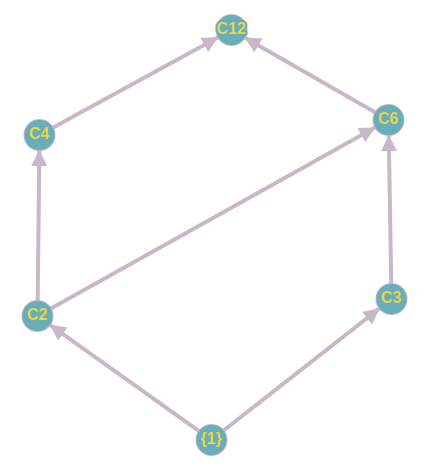
\includegraphics[scale=1,width=0.8\textwidth]{grafo.png}
\end{figure}

$H,K\in Sub(G)$ si $H\leq K$ y $\nexists H'\in Sub(G)$ con $H\leq H'\leq K$

\begin{equation*}
H\longrightarrow K \longrightarrow L
\end{equation*}
\end{enumerate}

\textbf{12-4-21} \\

\textbf{Demostración:} 
\begin{enumerate}[(1)]
\item $d\mid n, \quad d\geq 1, \quad \left\langle x^{\frac{n}{d}} \right\rangle$

Puesto que $(x^{\frac{n}{d}})=\frac{n}{mcd(n,\frac{n}{d})}=\frac{n}{mcd(n,s)}=\frac{n}{s}=d$ 

$\frac{n}{d}=s\Rightarrow n=sd$

Entonces $|\left\langle x^{\frac{n}{d}}\right\rangle|=d$, es decir, $\left\langle x^{\frac{n}{d}}\right\rangle=C_d$

\item $H\leq C_n, \quad H\neq \{1\}, \quad s=min\{r\geq 1/x^r\in H\}$

Debemos comprobar que $s\mid n$ y $\left\langle a^s \right\rangle=H$.

Puesto que $s\in \{r\geq 1/x^r\in H\}\Rightarrow x^s\in H\Rightarrow \left\langle x^s\right\rangle \leq H$ \\

Sea $x^m \in H$, dividimos $m$ entre $s$, $m=sq+t \quad 0\leq t<s$

\begin{gather*}
x^m=x^{sq}\cdot x^t \Rightarrow x^t=x^m\cdot (x^{sq})^{-1} \Rightarrow \\
\left. \begin{array}{c}
x^t\in H \\
0\leq t < s \\
s\:es\:el\:minimo\:de\:A
\end{array}\right\rbrace \Rightarrow t=0
\end{gather*}

Entonces $m=sq$ con lo que
\begin{equation*}
x^m=x^{sq}\in \left\langle x^s\right\rangle \Rightarrow H\leq \left\langle x^s\right\rangle
\end{equation*}

Por tanto $\left\langle x^s \right\rangle = H$. Puesto que $x^n=1\in H$, entonces $s\mid n$ por el mismo razonamiento anterior.

\begin{gather*}
H=\left\langle x^s\right\rangle \quad s\mid n \Rightarrow n=sd \Rightarrow s=\frac{n}{d} \\
H=\left\langle x^{\frac{n}{d}}\right\rangle
\end{gather*}

Los apartados (3) y (4) se dejan como ejercicios.
\end{enumerate}

\textbf{Ejercicio 28 (Relación 2):} $p$ un primo y $n\geq 1$

\begin{gather*}
C_{p^n}=\left\langle x/x^{p^n}=1\right\rangle \\
Div(p^n)=\{p^k/0\leq k \leq n\} \quad p^k \\
\updownarrow \qquad\qquad\qquad\qquad\qquad\qquad \downarrow \\
Sup(C_{p^n}) \qquad\qquad\quad \left\langle x^{\frac{p^n}{p^k}} \right\rangle = \left\langle x^{p^{n-k}} \right\rangle \\
Sub(C_{p^n})=\{\left\langle x^{p^{n-k}} \right\rangle=C_{p^k} / 0\leq k \leq n\} \\
C_{p^n}\rightarrow C_{p^{n-1}}\rightarrow C_{p^{n-2}} \rightarrow \ldots \rightarrow C_p \rightarrow \{1\}
\end{gather*}

\textbf{Ejercicio 27 (Relación 2):} Describir $Sub(S_3)$ y $Sub(D_4)$ \\

$Sub(S_3): \qquad S_3=\{id,(1\:2),(1\:3),(2\:3),(1\:2\:3),(1\:3\:2)\}$

Puesto que $|S_3|=6$ entonces sus posibles subgrupos tendrań 1, 2, 3 ó 6 elementos.

\begin{itemize}
\item De orden 1 es $\{1\}$

\item De orden 6 es $S_3$ 

\item De orden 2: todo grupo de orden 2 es cíclico generado por un elemento, luego hay tres subgrupo de orden 2

\begin{equation*}
C_2=\left\langle (1\:2)\right\rangle = \{id, (1\:2)\},\quad C_2'=\left\langle (1\:3)\right\rangle=\{id,(1\:3)\},\quad C_2''=\left\langle(2\:3)\right\rangle = \{id,(2\:3)\}
\end{equation*}

\item De orden 3: todo grupo de orden 3 es cíclico:

\begin{gather*}
C_3=\left\langle (1\:2\:3)\right\rangle = \{id,(1\:2\:3),(1\:2\:3)^2=(1\:3\:2)\}=\\
=\left\langle (1\:3\:2)\right\rangle=\{id,(1\:3\:2),(1\:3\:2)^2=(1\:2\:3)\}
\end{gather*}
\end{itemize}

$Sub(D_4):$
\begin{equation*}
D_4=\left\langle r,s|r^4=1=s^2\quad sr=r^3s\right\rangle=\{1,\,r,\,r^2,\,r^3,\,s,\,rs,\,r^2s,\,r^3s\}
\end{equation*}

$|D_4|=8$ y entonces buscamos subgrupos de orden 1, 2, 4 y 8.

\begin{itemize}
\item Orden 1 $\rightarrow \{1\}$ 

\item Orden 8 $\rightarrow D_4$ 

\item Orden 2 $\rightarrow$ Generador por elementos de orden 2 de $D_4$

\begin{gather*}
C_2=\left\langle r^2\right\rangle = \{1,\,r^2\} \qquad C_2'''=\left\langle rs\right\rangle = \{1,\,rs\} \\
C_2'=\left\langle s \right\rangle = \{1,\,s\} \qquad C_2^{iv}=\left\langle r^3s\right\rangle = \{1,\,r^3s\} \\
C_2''=\left\langle r^2s\right\rangle = \{1,\,r^2s\}
\end{gather*}

\item Orden 4: Como los grupos de orden 4 son, salvo isomorfismo, $C_4$ o tipo Klein. Los cíclicos de orden 4 son los generados por los elementos de orde 4 en $D_4$, que son $r$ y $r^3$.

\begin{equation*}
C_4=\left\langle r\right\rangle = \{1,\,r,\,r^2,\,r^3\}=\left\langle r^3\right\rangle
\end{equation*}

Para buscar los subgrupos en $D_4$ que sean tipo Klein, tenemos que buscar dos elementos de orden 2 que conmuten entre si

\begin{gather*}
r^2,\,s,\,rs,\,r^2s,\,r^3s \\
r^2,\,s \:tienen\:orden\:2 \qquad (sr^i=r^{-i}s,\:en\:el\:grupo\:diedrico) \\
sr^2=r^2s \qquad K=\{1,\,r^2,\,s,\,r^2s\}\leq D_4 \\
r^2,\, rs \:tienen\:orden\:2 \\
\left. \begin{array}{c}
r^2(rs)=r^{3s} \\
rsr^2=rr^2s=r^3s
\end{array} \right\rbrace \Rightarrow r^2(rs)=(rs)r^2 \\
K'=\{1,\,r^2,\,rs,\,r^3s\}
\end{gather*}
\end{itemize}

\textbf{13-4-21} \\

\textbf{Proposición:} Sea $C_n=\left\langle x/x^n=1\right\rangle$

\begin{enumerate}[(1)]
\item $\left\langle x^m\right\rangle = \left\langle x^{mcd(m,n)}\right\rangle$
\item $\left\langle x^{m_1},\,x^{m_2},\ldots,x^{m_k}\right\rangle = \left\langle x^{mcd(m_1,m_2,\ldots,m_k,n)}\right\rangle$
\end{enumerate}

\textbf{Demostración:}

\begin{enumerate}[(1)]
\item Sea $d=mcd(m,n)$. Tendremos que $n=ds$. Sabemos que existe un único subrgrupo cíclico de orden $s$ que es 

\begin{gather*}
\left\langle x^{\frac{n}{s}}\right\rangle = \left\langle x^d \right\rangle \\
|\left\langle x^m\right\rangle|=ord(x^m)=\frac{n}{mcd(n,m)}=\frac{n}{d}=s
\end{gather*}

Por tanto $\left\langle x^m\right\rangle = \left\langle x^d\right\rangle$

\item $N=\left\langle x^{m_1},\,x^{m_2},\ldots,\,x^{m_k}\right\rangle \leq C_n$. Sea $d=mcd(m_1,\,m_2,\ldots,\,m_k,n)$. Puesto que $d\mid m_i \Rightarrow x^{m_i}\in \left\langle x^d\right\rangle \quad 	\forall i=1,\ldots,k$, por tanto $N\leq \left\langle x^d\right\rangle$.

Por el teorema de Bezout, $\exists t_1,\,t_2,\ldots,\,t_n,\,t\in \mathbb{Z}$, tal que 
\begin{equation*}
d=m_1t_1+m_2t_2+\ldots+m_kt_k+nt
\end{equation*}

, entonces
\begin{equation*}
x^d=x^{m_1t_1}\cdot x^{m_2t_2}\ldots x^{m_kt_k}\in N
\end{equation*}

con lo que $\left\langle x^d\right\rangle \leq N$
\end{enumerate}

\section{Tema 4. Grupos Cocientes. Teoremas de Isomorfías.}

\textbf{Definición:} Sea $G$ un grupo y $N$ un subgrupo de $G$. Diremos que $N$ es un subgrupo normal de $G$
\begin{equation*}
aN=Na \qquad \forall a\in G
\end{equation*}

Es decir, las clases laterales a izquierda coinciden con las laterales a derecha. \\

\textbf{Ejemplos:}
\begin{enumerate}[(1)]
\item Si $G$ es abeliano, todo subgrupo suyo es normal

\item Para todo $G$, $\{1\}$ y $G$ son normales

\item Sea $G=D_4$ y $N=\left\langle r\right\rangle=\{1,\,r,\,r^2,\,r^3\}$
\begin{gather*}
D_4=\left\langle r,s/r^4=1=s^2,\:sr=r^3s\right\rangle \\
\left[ D_4:N\right] =\frac{|D_4|}{|N|}=\frac{8}{4}=2 \\
D_4/N=\{N,\,sN\}\quad N/D_4=\{N,Ns\} \\
sN=\{s,\,sr,\,sr^2,\,sr^3\}=\{s,\,r^3s,\,r^2s,\,rs\}=Ns
\end{gather*}

Por tanto $N\unlhd D_4$
\end{enumerate}

Sea $N=\left\langle s \right\rangle = \{1,\,s\}\leq D_4$, no es normal en $D_4$

\begin{equation*}
rN=\{r,\,rs\}\neq N_r=\{r,\,sr\}=\{r,\,r^3s\}
\end{equation*}

\textbf{Teorema:} Sea $G$ un grupo y $N \leq G$, son equivalentes los siguientes enunciados:

\begin{enumerate}[(1)]
\item $N$ es un subgrupo normal en $G$.

\item $aNa^{-1}=N\quad \forall a\in G$

\item $aNa^{-1}\leq N \quad \forall a \in G$
\end{enumerate}

Es decir, $N$ es un subgrupo normal de $G$ si y sólo si coincide con todos sus conjugados ó, si y sólo si contiene a todos sus conjutados. \\

Para $N\leq G$ y $a\in G$, el subgrupo 
\begin{equation*}
aNa^{-1}=\{axa^{-1}/x\in N\}
\end{equation*}

se llama el subgrupo conjugado de $N$ por el elemento $a$. \\

\textbf{Demostración:} $(1)\Rightarrow (2)\Rightarrow (3)$ Lo hace en clase. Fácil. 

$(3)\Rightarrow (1)$ Sea $a\in G$, tenemos que ver que 
\begin{equation*}
aN=Na
\end{equation*}

Lo vemos por doble inclusión. Sea $x\in aN\Rightarrow \exists n\in N$ tal que $x=an$. Entonces, $xa^{-1}=ana^{-1} \in aNa^{-1} \leq N \Rightarrow \exists n'\in N$ tal que $xa^{-1}=n'$, luego $x=n'a\in Na$. \\

Tenemos pues que $aN\leq Na$. \\

Sea $y\in Na\Rightarrow \exists m \in N$ tal que  $y=mc$. Entonces $a^{-1}y=a^{-1}ma \in a'Na\leq N \Rightarrow \exists m'\in N$ tal que $a^{-1}y\in m' \Rightarrow y=am'\in aN$. \\

Por tanto, $Na\leq aN$

$\hfill\square$ \\

\textbf{Ejemplo:}
\begin{enumerate}[(1)]
\item Sea $f:G\rightarrow G'$ un homomorfismo de grupos.
\begin{equation*}
Ker(f)=\{x\in G/f(x)=1\}
\end{equation*}

Sea $a\in G$ y $x\in Ker(f)$
\begin{equation*}
f(axa^{-1})=f(a)f(x)f(a)^{-1}=f(a)f(a)^{-1}=1 \Rightarrow axa^{-1}\in Ker(f)
\end{equation*}

Luego $aKer(f)a^{-1}\leq Ker(f) \quad \forall a\in G$, entonces $Ker(f)\unlhd G$

\item Sea $G=S_4$ y 
\begin{equation*}
K=\{id,\,(1\:2)(3\:4),\,(1\:3)(2\:4),\,(1\:4)(2\:3)\}
\end{equation*}

Sea $\alpha \in S_4$
\begin{equation*}
\alpha(1\:2)(3\:4)\alpha^{-1}=\alpha(1\:2)\alpha^{-1}\alpha(3\:4)\alpha^{-1}=\\
=(\alpha(1)\alpha(2))\cdot(\alpha(3)\alpha(4))\in K
\end{equation*}

por ser $\alpha$ biyectiva. \\

Análogamente, por el mismo razonamiento,
\begin{gather*}
\alpha(1\:3)(2\:4)\alpha^{-1}\in K,\:\alpha(1\:4)(2\:3)\alpha^{-1}\in K\\
\alpha id \alpha^{-1}=id\in K
\end{gather*}

Por tanto, $\alpha K\alpha^{-1}\in K \quad \forall\alpha\in S_4\Rightarrow K\unlhd S_4$
\end{enumerate}

\textbf{Proposición:} Sea $G$ un grupo y $X\subseteq G$ un subconjunto de $G$ no vacío. Sea $N=\left\langle X\right\rangle$
\begin{equation*}
N\unlhd G \Leftrightarrow axa^{-1}\in N \quad \forall a\in G,\: \forall x \in X
\end{equation*}

\textbf{Demostración:} $\Leftarrow)$ Obvio\\

$\Rightarrow)$ Sea $a\in G$ y sea 
\begin{equation*}
\varphi_a:G\rightarrow G \qquad \varphi(y):=aya^{-1}
\end{equation*}

Es fácil ver (ejercicio) que $\varphi_a$ es un homomorfismo de grupos.
\begin{gather*}
aNa^{-1}=(\varphi_{a_*})(N)=(\varphi_{a_*})(\left\langle X \right\rangle)=\\
=\left\langle (\varphi_{a_*})(X)\right\rangle=\left\langle aXa^{-1}\in N\right\rangle \leq N
\end{gather*}

Por tanto $N\unlhd G$

$\hfill\square$ \\

\textbf{Ejemplo:} $\forall n \geq 2 \quad A_n\unlhd S_n$. Para ello, utilizamos que $A_n$ está generado por 
\begin{equation*}
X=\{(x_1,\,x_2,\,x_3)/x_1,\,x_2,\,x_3\in\{1,\,2,\ldots,\,n\}\}
\end{equation*}

Sea $\alpha \in S_n$ y $(x_1,\,x_2,\,x_3)\in X$, entonces $\alpha(x_1,\,x_2,\,x_3)\alpha^{-1}=(\alpha(x_1)\alpha(x_2)\alpha(x_3))\in X \subseteq A_n$. \\

Por tanto, $A_n\unlhd S_n$
\begin{gather*}
(x\:y)(z\:t)=(x\:y\:z)(y\:z\:t) \\
(x\:y)(y\:z)=(x\:y\:z)
\end{gather*}

\textbf{14-4-21} \\

\textbf{Ejercicio 3 (Relación 3):} Sea $G$ un grupo finito y $H\leq G$ tal que $\left[G:H\right]=~2\Rightarrow~H\unlhd G$. \\

\textbf{Resolución:} $\left[G:H\right]=2\Rightarrow$
\begin{gather*}
G/H=\{H,aH\} \quad a\notin H\\
H/G=\{H,Ha\} 
\end{gather*}

Como $\left.\begin{array}{c}
G=H\cup aH \\
G=H\cup Ha
\end{array} \right.$ y ambas uniones son disjuntas $\Rightarrow$
\begin{equation*}
H=H\quad y \quad aH=Ha
\end{equation*}

Entonces $H\unlhd G$.

$\hfill\square$\\

Por tanto, $A_n\unlhd S_n\quad \forall n \geq 2$, pues $\left[S_n:A_n\right]=2$. También sabemos que en 
\begin{equation*}
D_n=\left\langle r,s/r^n=1=s^2,\quad sr=r^{n-1}s\right\rangle
\end{equation*}

el grupo $N=\left\langle r\right\rangle \unlhd D_n$ pues $\left[D_n:N\right]=\frac{|D_n|}{|N|}=\frac{2n}{n}=2$. \\

\textbf{Ejercicio 4 (Relación 3):} Describid el retículo de subgrupos de $A_4$.
\begin{gather*}
A_4=\{id,\,(1\:2)(3\:4),\,(1\:3)(2\:4),\,(1\:4)(2\:3),\,(1\:2\:3),\,(1\:3\:1), \\
(1\:2\:4),\,(1\:4\:2),\,(1\:3\:4),\,(1\:4\:3),\,(2\:3\:4),\,(2\:4\:3)\} \\
|A_n|=\frac{n!}{2} \qquad |A_4|=12
\end{gather*}

tendrá posiblemente subgrupos de orden 1, 2, 3, 4, 6 ó 12.

\begin{gather*}
orden\:2:\:\{(1\:2)(3\:4)\},\,\{(1\:3)(2\:4)\},\,\{(1\:4)(2\:3)\} \\
orden\:3:\:\{(1\:2\:4),\,(1\:4\:2)\},\{(1\:3\:4),\,(1\:4\:3)\},\{(2\:3\:4),\,(2\:4\:3)\} \\
orden\:4:\:no\:hay\:subgrupos\:isomorfos\:a\:C_4\:pero\:hay\:subgrupos\:de\:tipo\:Klein \\
K=\{id,\,(1\:2)(3\:4),\,(1\:3)(2\:4),\,(1\:4)(2\:3)\}\unlhd A_4 \\
orden\:6:\:no\:tiene\:subgrupos\:de\:orden\:6
\end{gather*}

Supongamos que $\exists N\leq A_4$ tal que $|N|=6$. Entonces $\left[A_4:N\right]=\frac{|A_4|}{|N|}=\frac{12}{6}=2\Rightarrow N\unlhd A_4$. Como $|N|=6$, $N$ ha de contener un ciclo de longitud $3$. Supongamos 
\begin{equation*}
(1\:2\:3)\in N\Rightarrow (1\:2\:3)^{-1}=(1\:3\:2)\in N
\end{equation*}

Sea $\alpha=(1\:2)(3\:4)\in A_4$, como $N\unlhd A_4$, entonces 
\begin{equation*}
\alpha(1\:2\:3)\alpha^{-1}=(2\:1\:4)=(1\:4\:2)\in N
\end{equation*}

Sea $\beta=(1\:2)(2\:4)\in A_4$, como $N\unlhd A_4$, entonces $\beta(1\:2\:3)\beta^{-1}=(3\:4\:1)=(1\:3\:4)\in N\Rightarrow(1\:3\:4)^{-1}=(1\:4\:3)\in N$.

Como $id\in N$, pues $N$ es un subgrupo, resulta $|N|=7 \downarrow$.\\

Los subgrupos normales de $A_4$ son, $\{1\}$, $A_4$ y $K$. Los de orden 2 y los de orden 3 no son normales en $A_4$
\begin{equation*}
C_2=\{id,\,(1\:2)(3\:4)\}\leq A_4
\end{equation*}

Sea $\alpha=(1\:2\:3)$, entonces
\begin{gather*}
\alpha(1\:2)(3\:4)\alpha^{-1}=\alpha(1\:2)\alpha^{-1}\alpha(3\:4)\alpha^{-1}=(2\:3)(1\:4)=(1\:4)(2\:3)\notin C_2 \\
\alpha C_2\alpha^{-1}\cancel{\leq} C_2\Rightarrow C_2 \cancel{\unlhd} A_4 \\
\left. \begin{array}{c}
C_2\leq K \\
K\:es\:abeliano
\end{array} \right\rbrace entonces\:C_2\unlhd K
\end{gather*}

\subsection{Grupo Cociente}

Sea $G$ un grupo y $N\unlhd G$. Consideramos
\begin{equation*}
G/N=\{aN/a\in G\}
\end{equation*}

Definimos en $G/N$ la siguiente operación binaria
\begin{gather*}
G/N\times G/N\longrightarrow G/N \\
(aN,\,bN)\longmapsto (aN)(bN):=abN
\end{gather*}

Por ser $N$ un subgrupo normal de $G$, esta operación está bien definida. En efecto
\begin{gather*}
\left. \begin{array}{c}
aN=a_1N \\
bN=b_1N
\end{array}\right\rbrace \overset{?}{\Rightarrow} abN=a_1b_1N \\
aN=a_1N\Leftrightarrow a_1^{-1}a\in N\Leftrightarrow \exists n\in N\:tal\:que\:a_1^{-1}a=n \Rightarrow a=a_1n \\
bN=b_1N\Leftrightarrow \exists m \in N\: tal\:que\:b=b_1m
\end{gather*}

Entonces $ab=a_1nb_1m$. Como $nb_1\in Nb_1 \overset{N\unlhd G}{=} b_1N\Rightarrow \exists n'\in N\:tal\:que\:nb_1=b_1n'$

Entonces $ab=a_1nb_1m=a_1b_1n'm \overset{n'm\in N}{\Rightarrow}(a_1b_1)^{-1}(ab)\in N\Rightarrow abN=~a_1b_1N$.

Resulta que $G/N$ con este producto tiene estructura de grupo, con uno dado por $1N=N$ y donde para cada $aN\in G/N$, $(aN)^{-1}=a^{-1}N$. Este grupo lo llamaremos grupo cociente de $G$ por $N$.

Se tiene un epimorfismo de grupo
\begin{equation*}
p:G\longrightarrow G/N\qquad p(a):=aN
\end{equation*}

que llamaremos la proyección canónica. \\

\textbf{Teorema:} Sea $f:G\rightarrow G'$ un homomorfismo de grupos. Sea $N\unlhd G$ tal que $N\leq Ker(f)$, entonces
\begin{enumerate}[(1)]
\item Existe un único homomorfismo
\begin{equation*}
\overline{f}:G/N\rightarrow G'
\end{equation*}

tal que $\overline{f}\cdot p=f$ (p proyección canónica).

\item $\overline{f}$ es epimorfismo $\Leftrightarrow$ $f$ es epimorfismo.

\item $\overline{f}$ es monomorfismo $\Leftrightarrow N=Ker(f)$
\end{enumerate}

$\overline{f}$ se llama el homomorfismo inducido por $f$ en el grupo cociente $G/N$ \\

\textbf{Demostración:} $f:G\rightarrow G'$, $N\unlhd G$ tal que $N\leq Ker(f) \quad G/N=\{aN/a\in G\}$ 

\begin{enumerate}[(1)]
\item Definimos
\begin{equation*}
\overline{f}:G/N\rightarrow G' \quad por\quad \overline{f}(aN):=f(a)
\end{equation*}

Veamos que $\overline{f}$ está bien definido. Si 
\begin{gather*}
aN=bN\Leftrightarrow b^{-1}a\in N\overset{N\leq Ker(f)}{\Rightarrow} b^{-1}a\in Ker(f) \\
\Rightarrow \left. \begin{array}{c}
f(b^{-1}a)=1=f(b)^{-1}f(a)
\end{array} \right\rbrace \Rightarrow f(a)=f(b)
\end{gather*}

Es fácil ver que $\overline{f}$ es un homomorfismo así como que $\overline{f}\circ p=f$. Supongamos que $g:G/N\rightarrow G'$ es un homomorfismo tal que $g\circ p=f$. Sea $aN\in G/N$, entonces $g(aN)=g(p(a))=(g\circ p)(a)=f(a)=\overline{f}(aN)$ 

\item Puesto que $Im(\overline{f})=Im(f)$
\begin{equation*}
\left. \begin{array}{c}
\overline{f}:G/N\rightarrow G'\\
\overline{f}(aN)=f(a)
\end{array} \right\rbrace
\end{equation*}

entonces $\overline{f}$ es epimorfismo $\Leftrightarrow$ $Im\overline{f}=G'\Leftrightarrow Imf=G'\Leftrightarrow f$ es epimorfismo.

\item $\overline{f}$ es monomorfismo $\Leftrightarrow N=Ker(f)$

$\Rightarrow)$ Tenemos que ver que $Ker(f)\leq N$. Sea $a\in Ker(f)\Rightarrow f(a)=1$. Como $\overline{f}(aN)=f(a)=1\Rightarrow aN\in Ker(\overline{f})\overset{\overline{f}\:monomorfismo}{=}\{N\}\Rightarrow aN=~N\Rightarrow~a\in~N$ \\

$\Leftarrow)$ Si $N=Ker(f)$ $\overline{f}:G/N\rightarrow G'$. Sea $aN\in G/N$ tal que $\overline{f}(aN)=~f(a)=~1$, entonces $a\in Ker(f)=N\Rightarrow aN=N$
\end{enumerate}

Así pues $Ker\overline{f}=\{N\}$ y $\overline{f}$ es monomorfismo.

$\hfill\square$\\

\textbf{Corolario:} (1º Teorema de Isomorfía)

Sea $f:G\rightarrow G'$ un homomorfismo de grupos. Entonces $f$ induce en isomorfismo
\begin{equation*}
G/Ker(f)\overset{\sim}{=} Imf\qquad aKer(\overline{f})\mapsto f(a)
\end{equation*}

\textbf{Demostración:} Consideramos $f:G\rightarrow Imf$ y aplicamos el teorema anterior a este homomorfismo tomando $N=Ker(f)$. Entonces $f$ induce un homomorfismo:
\begin{gather*}
\overline{f}:G/Ker(f)\rightarrow Imf \qquad \overline{f}(a\,Ker(f))=f(a) \\
\left. \begin{array}{c}
\overline{f}\:es\:epimorfismo\:por\:(2)\\
Como\:N=Ker(f),\:\overline{f}\:es\:monomorfismo\:por\:(3)
\end{array} \right\rbrace 
\overline{f}\:es\:isomorfismo
\end{gather*}

$\hfill\square$\\

\textbf{Ejercicio 12 (Relación 3):} $G$ y $H$ finitos y $mcd(|G|,\,|H|)=1$. Probar que si $f:G\rightarrow H$ es un homomorfismo, entonces $f(a)=1\quad \forall a\in G$. \\

\textbf{Resolución:}
\begin{equation*}
G/Ker(f)\overset{\sim}{=} Img(f) \qquad |G/Ker(f)|=|Img(f)|\Rightarrow |G|=|Ker(f)||Imf|
\end{equation*}

\begin{gather*}
\left. \begin{array}{c}
En\:particular\:|Imf|\:es\:un\:divisor\:de\:|G|\\
Imf\leq H\Rightarrow|Imf|\:es\:un\:divisor\:de\:|H|
\end{array} \right\rbrace = mdc(|G|,|H|)=1 \\
|Imf|=1\Rightarrow Imf=\{1\}\Rightarrow f(a)=1 \forall a \in G
\end{gather*}

\textbf{Corolario:} Si $f:G\rightarrow G'$ es un homomorfismo y $G$ y $G'$ son finitos, entonces $|G|=|Imf||Nucf|$ \\

\textbf{Proposición:} Sea $G$ un grupo y $N\unlhd G$. Entonces:
\begin{enumerate}[(1)]
\item Si $H\in Sub(G)$ tal que $N\leq H$ entonces $N\unlhd H$ y $H/N\in Sub(G/N)$.

\item Si $H_1,\,H_2\in Sub(G)$ tal que $N\unlhd H_i \quad i=1,\,2$, entonces $H_1/N=H_2/N\Leftrightarrow ~H_1=~H_2$.

\item Sea $L\in Sub(G/N)$. Entonces $\exists ! H\in Sub(G)$ tal que $N\unlhd H$ y $L=H/N$
\end{enumerate}

\textbf{Demostración:}
\begin{enumerate}[(1)]
\item Si $aNa^{-1}\leq N \quad \forall a\in G$ entonces $aNa^{-1}\leq N \quad \forall a\in H$ pues $H\leq G$, con lo que $N\unlhd H$. Podemos pues considerar $H/N\leq G/N$. Así $H/N\in Sub(G/N)$.

\item $\Leftarrow)$ Es obvio

$\Rightarrow)$ $H_1,\,H_2\leq G$ tal que $N\unlhd H_i\quad i=1,\,2$ tal que $H_1/N=H_2/N$. 

Sea $a\in H_1\Rightarrow aN\in H_1/N=H_2/N\Rightarrow \exists t\in H_2$ tal que $aN=tN\Leftrightarrow~t^{-1}a\in~N\leq~H_2$

\begin{equation*}
\left. \begin{array}{c}
t^{-1}a\in H_2 \\
t\in H_2
\end{array} \right\rbrace a=t(t^{-1}a)\in H_2
\end{equation*}

Tenemos que $H_1\leq H_2$. De la misma forma obtenemos que $H_2\leq H_1 \Rightarrow~H_2=~H_1$

\item $L\leq G/N$. Consideramos la proyección canónica $p:G\rightarrow G/N \quad p(a)=aN$. $L\leq G/N$ entonces $p^*(L)\leq G$. Sea 
\begin{equation*}
H=p^*(L)=\{a\in G/p(a)\in L\}=\{a\in G/aN\in L\}\leq G
\end{equation*}

Sea $a\in N\Rightarrow p(a)=aN=N\overset{L\leq G/N}{\in} L\Rightarrow a\in H$. Por tanto $N\leq H$. Veamos que $L=H/N$. Es claro que $H/N\leq L$. Recíprocamente, si $aN\in~L\Rightarrow a\in H\Rightarrow aN\in H$, es decir, $L\leq H/N$. La unicidad es consecuencia de (2).
\end{enumerate}

\textbf{Teorema} (2º Teorema de Isomorfía o Teorema del Doble Cociente): Sea $G$ un grupo y $N\unlhd G$ y sea $H\in Sub(G)$ tal que $N\leq H$. Entonces,
\begin{equation*}
H/N\unlhd G/N\Leftrightarrow H\unlhd G
\end{equation*}

Además en tal caso
\begin{equation*}
G/H\overset{\sim}{=}(G/N)(H/N)
\end{equation*}

\textbf{19-4-21} \\

\textbf{Demsotración:} $N\unlhd G$ y $H\leq G$ con $N\unlhd H\Leftrightarrow H\unlhd G$ y tenemos que ver que $H/N\unlhd G/N$. 

Sea $aN\in H/N$ y $xN\in G/N$, es decir, $a\in H$

\begin{equation*}
(xN)(aN)(xN)^{-1}=(xax^{-1})N\in H/N
\end{equation*}

Como $\left. \begin{array}{c}
a\in H\\
x\in G\\
H\unlhd G
\end{array}\right\rbrace \Rightarrow xHx^{-1} \leq H$, y por tanto $xax^{-1}\in H$ \\

Es decir, $\left. (xN)(H/N)^{-1}\leq H/N, \quad \forall xN\in G/N \right\rbrace\Rightarrow H/N\unlhd G/N$ \\

$\Rightarrow)$ Suponemos ahora que $H/N\unlhd G/N$
\begin{gather*}
G\overset{p}{\longrightarrow}G/N\overset{q}{\longrightarrow}(G/N)(H/N) \\
Sea \quad f=q\circ p:G\longrightarrow (G/N)/(H/N)
\end{gather*}

, y $p$ y $q$ proyecciones canónicas, con $f(a)=(aN)H/N$, entonces $f$ es un epimorfismo por ser composición de epimorfismos.

\begin{gather*}
Ker(f)=\{a\in G|\:f(a)=H/N\}=\\
=\{a\in G|\:(aN)H/N=H/N\}=\\
=\{a\in G|\:aN\in H/N\}
\end{gather*}

Veamos que $H=Ker(f)$ por doble inclusión. 

Es claro que $H\leq Ker(f)$.

Sea $a\in Ker(f)$ entonces $aN\in H/N\Rightarrow \exists b\in H$ tal que $aN=bN\Rightarrow$
\begin{equation*}
\Rightarrow \left. \begin{array}{c}
b^{-1}a\in N\leq H\\
b\in H
\end{array} \right\rbrace \Rightarrow a=b(b^{-1}a)\in H
\end{equation*}

, por tanto $Ker(f)\leq H$. Consecuentemente, $H=Ker(f)\Rightarrow H\unlhd G$. Además, aplicando el primer teorema de isomorfía a $f$, 
\begin{equation*}
G/Ker(f)\overset{\sim}{=} Im(f)
\end{equation*}

,es decir,
\begin{equation*}
G/H\overset{\sim}{=} (G/N)/(H/N)
\end{equation*}

pues $f$ es epimorfismo.

$\hfill\square$ \\

\textbf{Teorema:}(3 Teorema de Isomorfía)

Sea $G$ un grupo, y $N,\,K\in Sub(G)$ con $N\unlhd G$. Entonces
\begin{enumerate}[(1)]
\item $KN$ es un subgrupo de $G$ y $N\unlhd KN$

\item $K\cap N\unlhd K$ 

\item Existe un isomorfismo $K/(K\cap N)\overset{\sim}{=} KN/N$
\end{enumerate}

\textbf{Demostración:}

(1) Para demostrar que $KN\leq G$ basta con ver que $KN=NK$ y esta igualdad es inmediata puesto que $N\unlhd G$, por tanto $KN\in Sub(G)$.

Es claro que $N\leq KN\: (x\in N,\: x=1x\in KN)$ y $N\unlhd G$, entonces $N\unlhd KN$. \\

Veamos (2) y (3). Consideramos los siguientes homomorfismos.
\begin{equation*}
K\overset{i}{\hookrightarrow} G \overset{p}{\rightarrow} G/N
\end{equation*}

y sea
\begin{gather*}
g=p\circ i:K\longrightarrow G/N\\
g(a)=aN\qquad \forall a\in K \\
Ker(g)=\{a\in K/g(a)=N\}=\{a\in K/aN=N\}=\{a\in K/a\in N\}=K\cap N
\end{gather*}

y entonces $K\cap N\unlhd K$ y tenemos (2). \\

Además por el primer teorema de isomorfía aplicado a g,
\begin{gather*}
K/K\cap N\overset{\sim}{=} Im(g) \\
Im(g)=\{g(a)/a\in K\}=\{aN/a\in K\}\overset{?}{=}KN/N
\end{gather*}

Puesto que $K\leq N$, es claro que $Im(g)\leq KN/N$. Recíprocamente, sea $xN\in KN/N$, es decir, $x\in KN$, si $x\in KN\Rightarrow \exists a\in K$ y $\exists b\in N$ tal que $x=ab$. Entonces 
\begin{gather*}
xN=(ab)/N=(aN)(bN)\overset{b\in N}{=}(aN)N=aN\in Im(g),\:pues\:a\in K \\
K/K\cap N\overset{\sim}{=} KN/N \Rightarrow\\
\Rightarrow Im(g)=\{g(a)/a\in K\}=\{aN/a\in K\}=KN/N
\end{gather*}

\textbf{Ejercicio 14 (Relación 3):} $G$ grupo, $N\unlhd G$ tal que $N$ y $G/N$ son abelianos y $H\leq G$. Demostrar que existe $K\unlhd H$ tal que $K$ y $H/K$ son abelianos. \\
\begin{gather*}
G,\quad H,\,N\in Sub(G),\:N\unlhd G \\
N\cap H\unlhd H\quad y\quad NH/N\overset{\sim}{=}H/N\cap H\:(3\:Tª\:isomorfia)
\end{gather*}

Tomamos $K=N\cap H\unlhd H$, como $K\leq N$ y $N$ es abeliano $\Rightarrow$ $K$ abeliano. Por otro lado $H/K=H/N\cap H\overset{\sim}{=} HN/N\leq G/H$. Como $G/N$ es abeliano $\Rightarrow$ $HN/N$ es abeliano $\Rightarrow H/K$ es abeliano.

$\hfill\square$ \\

\textbf{Ejercicio 15 (Relación 3):} $G$ un grupo finito, $K,\,N\in Sub(G)$ con $N\unlhd G$. Suponemos que $|K|$ y $\left[G:N\right]$ son primos relativos. Demostrad que $K\leq N$. \\

\textbf{Resolución:} Sabemos que 
\begin{equation*}
K/K\cap N\overset{\sim}{=} KN/N\:(3\:Tª\:isomorfia)
\end{equation*}

entonces $\left[K:NK\right]=\left[KN:N\right]=r$. Como 
\begin{equation*}
KN/N\leq G/N\Rightarrow r=|KN/N| \mid |G/N|=\left[G:N\right]
\end{equation*}

Por otro lado
\begin{equation*}
r=\left[K:K\cap N\right]=\frac{|K|}{|K\cap N|}\Rightarrow |K|=r\cdot |K\cap N|\Rightarrow r\mid |K|
\end{equation*}

Como $mcd(|K|,\,\left[G:N\right])=1$, entonces $r=1$. Tenemos entonces que 
\begin{equation*}
|K/K\cap N|=1\Rightarrow K=K\cap N
\end{equation*}

con lo que $K\leq N$, lo que queríamos demostrar.

\textbf{20-4-21} \\

\textbf{Definición:} Sea $G$ un grupo. Se define el centro de G como
\begin{equation*}
Z(G)=\{a\in G/ax=xa\quad \forall x\in G\}
\end{equation*}

$Z(G)\unlhd G$ (Ejercicio 6, Relación 3).

$G$ es abeliano $\Leftrightarrow Z(G)=G$ \\

\textbf{Ejercicio 8 (Relación 3):} 2) Demostrar que $Z(A_3)=A_3$ y que $Z(A_n)=~\{id\} \quad \forall n \geq~4$

\begin{equation*}
A_3=\{id,\,(1\:2\:3),\,(1\:3\:2)\}=\left\langle (1\:2\:3)\right\rangle \quad es \quad abeliano
\end{equation*}

y entonces $Z(A_3)=A_3$ \\

Sea $n\geq 4$ y sea $\sigma \in A_n$, $\sigma \neq id$ entonces $\exists \alpha \in A_n$ tal que $\sigma \alpha \neq \alpha \sigma$.

Si $\sigma \neq id$, entonces $\exists i\in \{1,\,2\ldots,\,n\}$ tal que $\sigma(i)=j$ siendo $j\neq i$. Elegimos $k,\,l\in \{1,\,2,\ldots,\,n\}$ tal que $k\neq l$ y $\{k,\,l\}\cap \{i,\,j\}=\emptyset$ (podemos elegirlos porque $n\geq 4$). \\

Sea $\alpha=(j\:k\:l)\in A_n$
\begin{equation*}
\left. \begin{array}{c}
\sigma \alpha(i)=\sigma(i)=j\\
\alpha \sigma(i)=\alpha(j)=k
\end{array} \right\rbrace \Rightarrow \sigma\alpha(i)\neq \alpha\sigma(i)\Rightarrow \sigma\alpha\neq\alpha\sigma \Rightarrow \sigma\notin Z(A_n)
\end{equation*}

Consecuentemente $Z(A_n)=\{id\}$

\begin{enumerate}[1)]
\item $Z(S_2)=S_2\quad y \quad Z(S_n)=\{id\}$ para $n\geq 3$
\end{enumerate}

\textbf{Ejercicio 9 (Relación 3):} Demostrar que $Z(D_n)=\{1,\,r^m\}$ si $n=2m$, y $Z(D_n)=\{1\}$ si $m=2m+1$\\

a) $n=2m\quad D_n=\left\langle r,s/r^n=1=s^2,\quad sr=r^{-1}s\right\rangle=\{1,r,\ldots,r^{n-1},s,rs,\ldots,r^{n-1}s\}$

Observamos primero que $r^ks\notin Z(D_n) \quad \forall k=0,\ldots,n-1$
\begin{gather*}
r(r^ks)=r^{k+1}s \quad (r^ks)=r^kr^{-1}s=r^{k-1}s \\
r^{k+1}s=r^{k-1}s\Leftrightarrow r^{k+1}=r^{k-1} \Leftrightarrow r=r^{-1} \Leftrightarrow r^2=1 \Leftrightarrow ord(r)=2\neq n \downarrow \\
r(r^ks)\neq (r^ks)r \Rightarrow r^ks\notin Z(D_n) \quad \forall k=0,\ldots,n-1
\end{gather*}

¿Cuándo $r^k\in Z(D_n)$?

Obviamente $r^kr^j=r^jr^k \quad \forall j=0,\ldots,n-1$, por tanto decir que $r^k\in Z(D_n)$, es decir 
\begin{gather*}
r^k(r^js)=(r^js)r^k \quad \forall j=0,\ldots,n-1\\
r^{k+j}s=r^jr^{-k}s=r^{j-k}s\Leftrightarrow r^{k+j}=r^{j-k}\quad \forall j\Leftrightarrow r^k=r^{-k}\Leftrightarrow \\
\Leftrightarrow (r^k)^2=1\Rightarrow ord(r^k)=2
\end{gather*}

Sabemos que $ord(r^k)=\frac{n}{mcd(n,k)}$
\begin{gather*}
r^k\in Z(D_n)\Leftrightarrow \frac{n}{mcd(n,k)}=2\Leftrightarrow n=2mcd(n,k) \\
como\quad n=2m\Rightarrow 2m=2mcd(2m,k)\Rightarrow m=mcd(2m,k)\Rightarrow k=m \\
Z(D_{2m})=\{1,r^m\}
\end{gather*}

\textbf{Ejercicios 16-20:} Se refieren al grupo de automorfismos de un grupo.\\

\textbf{Definición:} Sea $G$ un grupo. Un automorfismo de $G$ es un isomorfismo
\begin{gather*}
f:G\longrightarrow G \\
Aut(G)=\{f:G\longrightarrow G/f\:es\:automorfismo\} \\
\end{gather*}

$Aut(G)$ con la composición es un grupo. \\

\textbf{Ejercicio 18 (Relacion 3):} Sea $n\geq 2$ y $C_n=\left\langle x /x^n=1\right\rangle =\{1,x,\ldots,x^{n-1}\}$.

Sea $G$ un grupo arbitrario. Demostrar que 
\begin{enumerate}[(1)]
\item Si $\theta:C_n\longrightarrow G$ es un homomorfismo de grupos con $\theta(x)=g \quad (g\in G)$, entonces
\begin{equation*}
ord(g)\mid n \quad y \quad \theta \in (x^k)=g^k \quad \forall k=0,\ldots,n-1
\end{equation*}

Puesto que $\theta$ es un homomorfismo,
\begin{gather*}
\theta(1)=1=\theta(x^n)=\theta(x)^n=g^n\\
\end{gather*}

Por tanto, $g$ es un elemento de $G$ de orden finito y además, $ord(g)\mid n$. 

\item Demostrar que para cada $g\in G$ tal que $ord(g)\mid n$ existe un único homomorfismo de grupos que lo denota por
\begin{equation*}
\theta_g:C_n\longrightarrow G \quad tal\:que\quad \theta_g(x)=g
\end{equation*}

Definimos $\theta_g:C_n\longrightarrow G$ por $\theta_g(x^k):=g^k\quad k=0,\ldots,n-1$. Veamos que $\theta_g$ es un homomorfismo.

$x^k,\,x^r\in C_n$ hemos de ver que $\theta_g(x^k\cdot x^r)=\theta_g(x^k)\cdot \theta_g(x^r)$
\begin{gather*}
\theta_g(x^k\cdot x^r)=\theta(x^{res(k+r;n)})=g^{res(k+r;n)}=g^s=g^{res(s;t)} \\
res(k+r;n)=s
\end{gather*}

Sea $ord(g)=t$ 
\begin{gather*}
\theta_g(x^k)\cdot \theta_g(x^r)=g^k\cdot g^r=g^{res(k+r;t)} \\
s=tq+h\quad h=res(s;t)\quad 0\leq h\leq t-1 \\
s=res(k+r;n)\quad entonces\quad k+r=nq'+s \quad 0\leq s	\leq n-1 \\
\Rightarrow res(k+r;t)=h=res(s;t)
\end{gather*}

Entonces $\theta_g(x^kx^r)=\theta_g(x^k)\cdot \theta_g(x^r)$. La unicidad es consecuencia de (1).

\item Sea $g\in G$ tal que $ord(g)\mid n$. Demostrar que
\begin{gather*}
\theta_g:C_n\longrightarrow G\quad es\:monomorfismo\Leftrightarrow ord(g)=n\\
Como\quad \theta_g:C_n\longrightarrow G \quad \theta_g(x^k)=g^k\quad \forall k
\end{gather*}

$\Rightarrow)$ Supongamos que $\theta_g$ es monomorfismo $\Rightarrow Ker(\theta_g)=\{1\}$. 

Sea $t=ord(g)$ entonces $g^t=1$. Entonces
\begin{equation*}
1=g^t=\theta_g(x^t)\Rightarrow x^t\in Ker(\theta_g)=\{1\}\Rightarrow x^t=1 \overset{ord(x)=n}{\Rightarrow} n\mid t
\end{equation*}

como $t\mid n\Rightarrow n=t$ \\

\textbf{21-4-21} \\

$\Leftarrow)\:ord(g)=n, \quad \theta_g:C_n\longrightarrow G,\quad \theta_g(x^k)=g^k$

Sea $x^k\in Ker(\theta_g)\Rightarrow \theta_g(x^k)=g^k=1\overset{ord(g)=n}{\Rightarrow} n\mid k$

\item Demostrar que existe un isomorfismo
\begin{equation*}
\mathcal{U}(\mathbb{Z}_n)\overset{\sim}{=} Aut(C_n)
\end{equation*}

dado por $r\longmapsto f_r:C_n\longrightarrow C_n,\quad f_r(x)=x^r$

En particular $Aut(C_n)$ es abeliano y tiene $\varphi(n)$ elementos ($\varphi$ función de Euler)
\begin{equation*}
\mathcal{U}(\mathbb{Z}_n)=\{r/1\leq r\leq n-1\quad y\quad mcd(n,r)=1\}
\end{equation*}

Entonces para $r\in \mathcal{U}(\mathbb{Z}_n)$, $x^r$ es un generador de $C_n$, pues $ord(x^r)~=~\frac{n}{mcd(n,r)}~=~n$. Por (2) y (3) $f_r:C_n\longrightarrow C_n \quad f_r(x)=x^r\:(f_r(x^k)=x^{kr})$, es un monomorfismo. 

Como $Im(f_r)=\left\langle f_r(x)\right\rangle =\left\langle x^r\right\rangle =C_n$, entonces $f_r$ es también epimorfismo, y por lo tanto es un isomorfismo. \\

Tenemos pues una aplicación 
\begin{gather*}
f:\mathcal{U}(\mathbb{Z}_n)\longrightarrow Aut(C_n) \\
r\longmapsto f_r
\end{gather*}

f es un homomorfismo de grupos
\begin{gather*}
f(rs)=f_{rs}:C_n\longrightarrow C_n \qquad
f(r)\circ f(s)=f_r\circ f_s: C_n\longrightarrow C_n \\
f_r\circ f_s(x)=f_r(x)=x^{rs}=x^{res(r\cdot s;n)}=f_{res(r\cdot s;n)}(x)=f(rs)
\end{gather*}

Por (1) y (2) es fácil ver que $f$ es un isomorfismo.
\end{enumerate}

\textbf{Ejercicio 19 (Relación 3):} Describir $Aut(C_8)$ y demostrar que es isomorfo al grupo de Klein.
\begin{gather*}
Aut(C_8)\overset{\sim}{=}\mathcal{U}(\mathbb{Z}_8)=\{1,3,5,7\}\\
Aut(C_8)=\{f_1,f_3,f_5,f_7\} \\
f_k:C_5\longrightarrow C_8 \quad f_k(x)=x^k \quad k=1,3,5,7
\end{gather*}

Para $k=1$, $f_1=id$, $f_3,\,f_5,\,f_7$ tienen orden 2
\begin{equation*}
(f_3^2)(x)=f_3(f_3(x))=f_3(x^3)=(x^3)^3=x^9=x\Rightarrow f_3^2=id\Rightarrow ord(f_3)=2=ord(f_5)=ord(f_7)
\end{equation*}

\textbf{Ejercicio 20 (Relación 3):} $Aut(\mathbb{Z}_2\times \mathbb{Z}_2)\overset{\sim}{=} S_3$

$\mathbb{Z}_2\times \mathbb{Z}_2\overset{\sim}{=}$ al grupo de Klein. Trabajamos con el grupo de Klein de forma abstracta.
\begin{gather*}
K=\{1,a_1,a_2,a_3\}\quad a_i^2=1\quad i=0,1,2,3 \\
a_ia_j=a_k\quad con\quad k\neq i,j\neq 1\\
Aut(K)\overset{\sim}{=} S_3
\end{gather*}

Sea $\alpha \in S_3 \longrightarrow \left. \begin{array}{c}f_\alpha:K\longrightarrow K \\
f_\alpha(1)=1\\
f_\alpha(a_i)=a_{\alpha(i)}
\end{array} \right.$ biyectiva. 

$f_\alpha$ es un homomorfismo y entonces un autormorfismo.
\begin{gather*}
S_3\rightarrow Aut(K)\\
\alpha \longmapsto f_\alpha
\end{gather*}

$f$ es un isomorfismo. 

\subsection{Producto Directo de Grupos:}
\textbf{Definición:} Sea $G_1,G_2,\ldots,G_n$ ($n\geq 2$) grupos. Definimos su producto directo como el grupo cuyos elementos son los del producto cartesiano
\begin{equation*}
\prod_{i=1}^n G_i=G_1\times \ldots \times G_n=\{(x_1,x_2,\ldots,x_n)/x_i\in G_i\quad \forall i=1,2,\ldots,n\}
\end{equation*}

y con operación definida como sigue
\begin{equation*}
(x_1,\ldots,x_n)\cdot (y_1,\ldots,y_n):=(x_1y_1,x_2y_2,\ldots,x_ny_n)
\end{equation*}

Es fácil ver que en efecto $\prod_{i=1}^n G_i$ es un grupo con uno la n-tupla $(1,1,\ldots,1)$ (donde cada uno es el de su correspondiente $G_i$), y donde
\begin{equation*}
(x_1,\ldots,x_n)^{-1}=(x_1^{-1},x_2^{-1},\ldots,x_n^{-1})
\end{equation*}

Se tiene para cada $k=1,\ldots,n$ homomorfismo
\begin{equation*}
P_k:\prod_{i=1}^n G_i\longrightarrow G_k\qquad P_k(x_1,\ldots,x_n)=x_k
\end{equation*}

que se llama proyección k-ésima. También se tiene un homomorfismo
\begin{equation*}
j_k:G_k\longrightarrow \prod_{i=1}^n G_i \qquad j_k(x_k)=(1,\ldots,x_k,\ldots,1)
\end{equation*}

que se llama proyección k-ésima.

Es claro que las proyecciones son epimorfismos y las inyecciones son monomorfismos. Además se verifica
\begin{itemize}
\item $G_k=Im(P_k)\qquad \forall k=1,\ldots,n$
\item $Im(j_k)\unlhd \prod_{i=1}^n G_i \qquad \forall k=1,\ldots,n$

Así, $G_k$ es isomorfo a un subgrupo normal del producto directo.
\item Sea dado $H_k\in Sub(G_k)$ para cada $k=1,\ldots,n$, entonces $\prod{k=1}^n H_k$ es un subgrupo de $\prod_{k=1}^n G_k$
\end{itemize}

\textbf{Proposición:} Sean $G_1,G_2,\ldots,G_n$ grupos finitos, entonces
\begin{enumerate}[(1)]
\item $\prod_{i=1}^n G_i$ es también finito y 
\begin{equation*}
|\prod_{i=1}^n G_i|=\prod_{i=1}^n |G_i|
\end{equation*}

\item Sea $(x_1,\ldots,x_n)\in  \prod_{i=1}^n G_i$, entonces 
\begin{equation*}
ord((x_1,x_2,\ldots,x_n))=mcm(ord(x_1),ord(x_2),\ldots,ord(x_n))
\end{equation*}

Supongamos que $mcd(|G_i|,|G_j|)=1 \quad \forall i\neq j$

\item Si cada $G_i$ es cíclico entonces $\prod_{i=1}^n G_i$ es cíclico.

\item Si $L\leq \prod_{i=1}^n G_i$ entonces existe $H_1\leq G_1,H_2\leq G_2,\ldots ,H_n\leq G_n$ tal que
\begin{equation*}
L=\prod_{i=1}^n H_i
\end{equation*}
\end{enumerate}

\textbf{Demostración:} (2) $(x_1,x_2,\ldots,x_k)\in \prod_{i=1}^k G_i$ y sea $t_i=ord(x_i)$, $i~=~1,\ldots,n$.

Sea $t=mcm(t_1,t_2,\ldots,t_n)$
\begin{equation*}
(x_1,x_2,\ldots,x_n)^t=(x_1^t,x_2^t,\ldots,x_n^t)\overset{\left.\begin{array}{c}
ord(x_i)=t_i \\
t_i\mid t \quad \forall i
\end{array} \right.}{=} (1,1,\ldots,1)
\end{equation*}

Supongamos $m\geq 1$ tal que
\begin{equation*}
\left. \begin{array}{c}
(x_1,x_2,\ldots,x_n)^m=(1,1,\ldots,1)\\
(x_1^m,x_2^m,\ldots,x_n^m)
\end{array} \right\rbrace \Rightarrow x_i^m=1 \quad \forall i=1,\ldots,n
\end{equation*}

como $ord(x_i)=t_i\Rightarrow t_i\mid m \quad \forall i=1,\ldots,n$ y como $t=mcm(t_1,\ldots,t_n)\Rightarrow~t\mid~m$

Luego $ord(x_1,x_2,\ldots,x_n)=mcm(ord(x_1),\ldots,ord(x_n))$ \\

(3) $mcd(|G_i|,|G_j|)=1\quad \forall i\neq j$. Supongamos que $G_i=\left\langle a_i\right\rangle \quad i=1,\ldots,n$, y consideramos el elemento $a=(a_1,a_2,\ldots,a_n)\in \prod_{i=1}^n G_i$

Por (2)
\begin{gather*}
ord(a)=mcm(ord(a_1),\ldots,ord(a_n))= \\
=mcm(|G_1|,\ldots,|G_n|)=|G_1||G_2|\ldots|G_n| \\
\end{gather*}

Entonces $\left\langle a \right\rangle = \prod_{i=1}^nG_i$ y entonces es cíclico. \\

(4) $mcd(|G_i|,|G_j|)=1\quad \forall i\neq j$. Hacemos inducción en n.

Caso $n=2$. $L\leq G_1\times G_2$, queremos buscar $H_1\leq G_1$ y $H_2\leq G_2$ tal que $L=H_1\times H_2$. Consideramos
\begin{gather*}
p_1:G_1\times G_2\longrightarrow,\qquad (x_1,x_2)\longmapsto x_1 \\
p_2:G_1\times G_2\longrightarrow,\qquad (x_1,x_2)\longmapsto x_2
\end{gather*}

Sea $H_1=(P_1)_*(L)\leq G_1 \qquad H_2=(P_2)_*(L)\leq G_2$.

Si $(x_1,x_2)\in L\Rightarrow \left\lbrace \begin{array}{c}
P_1(x_1,x_2)=x_1\in (P_1)_*(L)=H_1\\
P_2(x_1,x_2)=x_2\in (P_2)_*(L)=H_2
\end{array} \right\rbrace \Rightarrow (x_1,x_2)\in~H_1\times~H_2$ 

Por tanto, $L\leq H_1\times H_2$ \\

Recíprocamente, $r=|G_1|,\quad s=|G_2| \quad mcd(r,s)=1$, elegimos $a,b\in \mathbb{Z}$ tal que $1=ar+bs$.

Sea $x_1\in H_1=(P_1)_*(L)$ entonces $\exists y_2\in G_2$ tal que $(x_1,y_2)\in L$
\begin{gather*}
(x_1,y_2)\in L\Rightarrow (x_1,y_2)^{bs}\in L \\
(x_1,y_2)^{bs}=(x_1^{bs},y_2^{bs})=(x_1^{bs},1)=(x_1^{1-ar},1)=(x_1^1\cdot x_1^{-ar},1)=(x_1,1)\\
y_2\in G_2\Rightarrow ord(y_2)\mid |G_2|=s \qquad x_1\in G_i \Rightarrow ord(x_1)\mid |G_1|=r
\end{gather*}

Así si $x_1\in H_1$ entonces $(x_1,1)\in L$. Análogamente, si $x_2\in H_2\Rightarrow (1,x_2)\in L$. \\

Sea $(x_1,x_2)\in H_1\times H_2 \Rightarrow x_1\in H_1 \quad y\quad x_2\in H_2$
\begin{equation*}
\Rightarrow (x_1,1),(1,x_2)\in L\Rightarrow (x_1,1)(1,x_2)=(x_1,x_2)\in L
\end{equation*}

Así $L=H_1\times H_2$.

Sea n>2, y el resultado cierto para n-1. Sea
\begin{equation*}
L\leq \prod_{i=1}^nG_i=\prod_{i=1}^{n-1} G_i\times G_n
\end{equation*}

como $mcd(|\prod_{i=1}^nG_i|,|G_n|)=1$, por el caso $n=2$
\begin{equation*}
\exists K\leq \prod_{i=1}^n G_i \quad y \quad \exists H_n\leq G_n \quad tal\:que\quad L=K\times H_n
\end{equation*}

Por hipótesis de inducción si $K\leq \prod_{i=1}^{n-1}G_i,\quad \exists H_1\leq G_i,\quad i=1,\ldots,n-1$ tal que 
\begin{equation*}
K=\prod_{i=1}^{n-1}H_i
\end{equation*}

, combinando, obtenemos que $L=H_1\times \ldots \times H_n$. \\

\textbf{Corolario:} Sean $n,m\geq 1$
\begin{equation*}
C_n\times C_m\overset{\sim}{=} C_{nm}\Leftrightarrow mcd(n,m)=1
\end{equation*}

Supongamos un grupo $G$ y $H_1,H_2,\ldots,H_n\in Sub(G)$. Consideramos $H_1~\times~ H_2~\times~\ldots~\times~H_n$. Tenemos una aplicación 
\begin{gather*}
\phi:H_1\times H_2\times \ldots \times H_n\longrightarrow G \\
\phi(x_1,x_2,\ldots,x_n):=x_1x_2\ldots x_n\in G
\end{gather*}

Se verifica \\

\textbf{Proposición:}
\begin{gather*}
\phi\:es\:un\:isomorfismo\Leftrightarrow\left\lbrace \begin{array}{c}
(a)\: H_i\unlhd G\quad \forall i=1,\ldots,n \\
(b)\: H_1H_2\ldots H_n=G\\
(c)\: (H_1\ldots H_{i-1})\cap H_i=\{1\} \quad \forall i=2,\ldots,n
\end{array}\right. \\
\left( n=2\quad \phi\:es\:isomorfismo \Leftrightarrow\left\lbrace \begin{array}{c}
(a)\: H_1\unlhd G\quad H_2\unlhd G  \\
(b)\: H_1H_2=G\\
(c)\: (H_1)\cap H_2=\{1\}
\end{array}\right. \right)
\end{gather*}

En estas condiciones se dice que el grupo es producto interno de los subgrupos $H_1,H_2,\ldots,H_n$. \\

\textbf{Demostración:} $\Rightarrow)$ $\phi:H_1\times \ldots \times H_n\longrightarrow G \qquad \phi(x_1\ldots x_n)=x_1\ldots x_n$ es isomorfismo. En particular es epimorfismo y entonces
\begin{equation*}
Im(\phi)=H_1H_2\ldots H_n=G\quad y\:se\:tiene\:(b)
\end{equation*}

\textbf{Ejercicio:} Sea $f:G\longrightarrow G'$ un homomorfismo d grupo y $N\unlhd G$. Demostrad que $f_*(N)\unlhd Im(f)$. \\

Entonces como para cada $k=1,\ldots,n$
\begin{equation*}
Im(j_k)\unlhd \prod_{i=1}^n H_i\Rightarrow \phi_*(Im(j_k))=H_k\unlhd Im(\phi)=G
\end{equation*}

$j_k:H_k\longrightarrow \prod_{i=1}^n H_i$ la k-ésima inyección canónica. Por tanto se tiene (a). \\

\textbf{26-4-21} \\

Veamos (c). Sea $x\in (H_1\ldots H_{i-1})\cap H_i\quad 2\leq i\leq n-1$.

Como $x\in H_1H_2\ldots H_{i-1}$, existirán $h_1\in H_1,\ldots,h_{i-1}\in H_{i-1}$ tal que $x~=~h_1\ldots h_{i-1}$. 

Entonces $x=\phi((h_1,h_2,\ldots,h_{i-1},1,\ldots,1))$ \\

Como $x\in H_i$, podemos considerar el elemento
\begin{gather*}
(1,1,\ldots,1,x,1,\ldots,1)\in H_1\times H_2\times \ldots \times H_n \quad y\\
\phi((1,1,\ldots,1,x,1,\ldots,1))=x
\end{gather*}

Entonces como $\phi$ es monomorfismo, tendremos que 
\begin{gather*}
(h_1,h_2,\ldots,h_{i-1},1,\ldots,1)=(1,1,\ldots,1,\overbrace{x}^{i-esima\:posicion},1\ldots,1) \\
\Rightarrow h_i=1\quad \forall i \quad y \quad x=1
\end{gather*}

Tenemos entonces que $(H_1\ldots H_{i-1})\cap H_i=\{1\} \quad 2\leq i \leq n$ \\

$\Leftarrow)$ Supongamos que se verifican (a), (b) y (c). Queremos demostrar que
\begin{equation*}
\phi:H_1\times \ldots\times H_n\longrightarrow G\qquad \phi(h_1,h_2,\ldots,h_n)=h_1h_2\ldots h_n
\end{equation*}

es isomorfismo.

Primero veamos que $\forall i \neq j$, los elementos de $H_i$ conmutan con los elementos de $H_j$. 

Supongamos que $i<j$ y sea $h_i\in H_i$, $h_j\in H_j$. Consideramos el elementos $a=h_ih_jh_i^{-1}h_j^{-1}$ \\

Como $H_i \unlhd G$ entonces $\left. \begin{array}{c}
h_jh_i^{-1}h_j^{-1}\in H_i\\
h_i\in H_i
\end{array} \right\rbrace \Rightarrow a\in H_i$ \\

Como $H_j\unlhd G$ entonces $\left. \begin{array}{c}
h_ih_jh_i^{-1}\in H_j \\
h_j^{-1}\in H_j
\end{array} \right\rbrace \Rightarrow a\in H_j$ \\

Por tanto $a\in H_i\cap H_j$. Si $i<j\Rightarrow H_i\leq H_1H_2\ldots H_{j-1} \}\Rightarrow a\in H_1H_2\ldots H_{j-1}\cap~H_j$ \\

(Ejercicio: Sean $H,K\in Sub(G) \left.\begin{array}{c}
H\subseteq HK \\
K\subseteq HK
\end{array} \right.$) \\

Entonces utilizando (c), $a=1$. Es decir,
\begin{equation*}
h_ih_jh_i^{-1}h_j^{-1}=1\Rightarrow h_ih_j=h_jh_i
\end{equation*}
 
Veamos primero que $\phi$ es homomorfismo
\begin{gather*}
\phi((h_1,h_2,\ldots,h_n)(k_1,k_2,\ldots,k_n))=\phi((h_1k_1,h_2k_2,\ldots,h_nk_n))=\\
=h_1k_1h_2k_2\ldots h_nk_n=h_1h_2k_1k_2h_3k_3\ldots h_nk_n=h_1h_2h_3k_1k_2k_3\ldots h_nk_n=\\
=h_1h_2\ldots h_nk_1k_2\ldots k_n=\phi((h_1,h_2,\ldots,h_n))\cdot \phi((k_1,k_2,\ldots,k_n))
\end{gather*}

Por definición de $\phi$
\begin{equation*}
Im(\phi)=H_1H_2\ldots H_n\overset{(b)}{=} G\Rightarrow\phi \quad es\:epimorfismo
\end{equation*}

Sea $(h_1,h_2,\ldots,h_n)\in Ker(\phi)\Rightarrow \phi((h_1,\ldots,h_n))\Rightarrow 1$, es decir, 
\begin{equation*}
h_1h_2\ldots h_n=1\Rightarrow h_1h_2\ldots h_{n-1}=h_n^{-1}\in (H_1\ldots H_{n-1})\cap H_n
\end{equation*}

que por (c) $\Rightarrow h_n=1$ y $h_1h_2\ldots h_{n-1}=1\Rightarrow h_1h_2\ldots h_{n-2}=h_{n-1}^{-1}\in~(H_1\ldots H_{n-2})\cap~H_{n-1}$, que por (c) $\Rightarrow h_{n-1}=1$ y $h_1h_2\ldots h_{n-2}=1$. 

En definitiva, en un número finito de pasos, llegamos a que 
\begin{equation*}
h_1=h_2=\ldots=h_n=1,\quad es\:decir,\quad(h_1,h_2,\ldots,h_n)=(1,1,\ldots,1)
\end{equation*}

y $\phi$ es monomorfismo. \\

\textbf{Ejercicios 21-32:} Ejercicios de producto directo. \\

\textbf{Ejercicio 21 (Relación 3):} $S_3,\:C_{p^n}$ (con p primo) y $\mathbb{Z}$ no son producto directo internos de subgrupos propios
\begin{equation*}
S_3\overset{subgrupos\:propios}{\longrightarrow} A_3\unlhd S_3,\:\left\langle (1\:2)\right\rangle \cancel{\unlhd}S_3,\:\left\langle(1\:3)\right\rangle \cancel{\unlhd} S_3,\:\left\langle (2\:3)\right\rangle \cancel{\unlhd} S_3
\end{equation*}

Luego no existe subgrupos tal que $S_3=K\cdot G$ con $K,G\in Sub(S_3)$ y $K\unlhd S_3$ y $G\unlhd S_3$. \\

$C_p\leq C_{p^2}\leq \ldots \leq C_{p^{n-1}} \qquad (H\leq K\Rightarrow HK=K)$. Nunca dará $C_{p^n}$, pues usaríamos un subgrupo impropio. \\

$\mathbb{Z}\longrightarrow$ si $\{0\}\neq H\leq \mathbb{Z}$, entonces $\exists n>1$ tal que $H=n\mathbb{Z}$. En efecto sea $n=min\{x>0/x\in H\}\neq \emptyset$. Como $H\leq \mathbb{Z}$, $n>1$ (pues si $n=1$, entonces $H=\mathbb{Z}$).

Veamos que $H=n\mathbb{Z}$. Puesto que $n\in H\Rightarrow n\mathbb{Z}\leq H$. \\

Recíprocamente, sea $x\in H$, dividimos $x$ entre $n$,
\begin{gather*}
x=nq+r\qquad 0\leq r<n \\
\left. \begin{array}{c}
r=x-nq\in H \\
0\leq r<n
\end{array}\right\rbrace \Rightarrow r=0
\end{gather*}

con lo que $x=nq \in n\mathbb{Z}$

\begin{gather*}
n\mathbb{Z},\:m\mathbb{Z}\quad n\mathbb{Z}+m\mathbb{Z}=mcd(n,m)\mathbb{Z} \\
n\mathbb{Z}+m\mathbb{Z}=mcm(n,m)\mathbb{Z}
\end{gather*}

\textbf{27-4-21} \\

\section{Tema 5. Grupos Resolubles (Solubles)}

\textbf{Definición:} Sea $G$ un grupo. Una cadena de subgrupos de $G$ en la forma
\begin{equation*}
\{1\}=H_0\unlhd H_1\unlhd \ldots \unlhd H_{n-1}\unlhd H_n=G
\end{equation*}

la llamaremos serie normal de $G$. \\

Cada $H_i$ se llama término i-ésimo de la serie, con $i=0,\ldots,n$.

Cada $H_i/H_{i-1}$ se llama factor i-ésimo de la serie, con $i=1,\ldots,n$

La serie se dice propia si $H_{i-1}\unlhdneq H_i\quad \forall i=1,\ldots,n$ (es decir, todas las inclusiones son propias). En tal caso, diremos que la serie tiene longitud $n$. \\

Dadas dos series,
\begin{gather*}
\{1\}=H_0\unlhd H_1\unlhd \ldots \unlhd H_{n-1}\unlhd H_n=G \tag{1} \\
\{1\}=K_0\unlhd K_1\unlhd \ldots \unlhd K_{m-1}\unlhd K_m=G \tag{2}
\end{gather*}

, diremos que la serie (2) es un refinamiento de la serie (1) si se verifica
\begin{enumerate}[\bfseries (i)]
\item $n\leq m$
\item Para cada $j\in \{0,\ldots,n\}$ existe un $r\in \{0,\ldots,m\}$ tal que $H_j=K_r$ (es decir, todos los grupos de la serie (1) aparecen en la serie (2))
\end{enumerate}

Si $n<m$, es decir, la serie (2) tiene más grupos que la serie (1), diremos que el refinamiento es propio. \\

\textbf{Ejemplo:} $G=S_4$

Son series normales propias de $S_4$
\begin{gather*}
\{id\}\unlhd A_4\unlhd S_4 \\
\{id\}\unlhd K\unlhd A_4\unlhd S_4\qquad K=\{id,(1\:2)(3\:4),(1\:3)(2\:4),(1\:4)(2\:3)\} \\
\{id\}\unlhd C_2\unlhd K\unlhd A_4\unlhd S_4 \qquad C_2=\left\langle (1\:2)(3\:4)\right\rangle =\{id,(1\:2)(3\:4)\}
\end{gather*}

La tercera es un refinamiento propio de la primera y de la segunda.

La segunda es un refinamiento propio de la primera. 

La primera tiene longitud 2, la segunda tiene longitud 3 y la tercera tiene longitud 4. \\

\textbf{Notemos:} que en una serie normal de un grupo $G$
\begin{equation*}
\{1\}\unlhd H_1\unlhd \ldots \unlhd H_{n-1}\unlhd H_n=G
\end{equation*}

$H_{i-1}$ es normal en $H_i$, pero no tiene porque ser normal en $H_j$ para $j\geq i+1$ \\

\textbf{Definición:} Sea $G$ un grupo. Una serie normal propia de $G$ que no admite refinamientos propios, la llamaremos una serie de composición de $G$.

A los factores de una serie de composición los llamaremos factores de composición de $G$. \\

\textbf{Nota:} No todo grupo tiene series de composición.

Por ejemplo $\mathbb{Z}$ no tiene series de composición, porque cualquier serie normal propia de $\mathbb{Z}$ puede refinarse propiamente. 

En efecto sea
\begin{equation*}
\{0\}=H_0\unlhdneq H_1\unlhdneq \ldots \unlhdneq H_n=\mathbb{Z}
\end{equation*}

Si $n=1$, $\{0\}=H_0\unlhdneq H_1=\mathbb{Z}$, consideramos $K=m\mathbb{Z}$, $m\geq 2$, entonces
\begin{equation*}
\{0\}=H_0\unlhdneq K\unlhdneq H_1=\mathbb{Z}
\end{equation*}

es un refinamiento propio de la serie. \\

Si $n>1$ entonces $H_1\unlhdneq \mathbb{Z}$, $H_1\neq \{0\}$ entonces $H_1=m\mathbb{Z}$ para $m\geq 2$

Consideramos $K=2m\mathbb{Z}$, entonces
\begin{equation*}
\{0\}=H_0\unlhdneq K\unlhdneq H_1 \unlhdneq H_2\unlhdneq \ldots \unlhdneq H_n=\mathbb{Z}
\end{equation*}

es un refinamiento de la serie dada. \\

\textbf{Definición:} Un grupo $G$ diremos que es simple si no es trivial y no admite subgrupos normales propios o, en otros términos, sus únicos subgrupos normales son $\{1\}$ y $G$. \\

En el caso abeliano se tiene

\textbf{Proposición:} Sea $G$ un grupo abeliano. $G$ es simple $\Leftrightarrow G$ es finito de orden número primo. \\

\textbf{Demostración:} $\Leftarrow)$ $|G|=p$, p primo $\Rightarrow G\overset{\sim}{=} C_p=\left\langle x/x^p=1\right\rangle$.

Si $H\leq G\Rightarrow |H|\mid |G|=p\Rightarrow \left\lbrace \begin{array}{c}
|H|=1\Rightarrow H=\{1\}\\
|H|=p\Rightarrow H=G
\end{array} \right.$ \\

$\Rightarrow)$ $G$ es simple y abeliano entonces $G$ no tiene subgrupos propios. Como $G$ no es trivial, elegimos $x\in G$, $x\neq 1$ y consideramos $\left\langle x \right\rangle$
\begin{equation*}
\left. \begin{array}{c}
\{1\}\neq \left\langle x\right\rangle \unlhd G \\
G\quad simple
\end{array}\right\rbrace \Rightarrow G=\left\langle x\right\rangle
\end{equation*}

Supongamos $ord(x)=\infty$, en ese caso $G\overset{\sim}{=} \mathbb{Z}$, que no es simple. Por tanto, necesariamente $ord(x)$ es finito. \\

Supongamos $ord(x)=m$. Como $G=\left\langle x\right\rangle$ entonces
\begin{equation*}
|G|=|\left\langle x \right\rangle |=ord(x)=m
\end{equation*}

y así $G$ es un grupo finito.

Sea $n\in \mathbb{Z}$, $n\mid m$ ($n>0$) y consideramos el elemtnos $x^n\in \left\langle x \right\rangle =G$ y el subgrupo $\left\langle x^n\right\rangle$
\begin{equation*}
\left. \begin{array}{c}
\left\langle x^n\right\rangle \unlhd G\\
G\quad es\:simple
\end{array}\right\rbrace \Rightarrow \left\lbrace \begin{array}{c}
\left\langle x^n \right\rangle=\{1\} \\
\left\langle x^n \right\rangle = G =\left\langle x \right\rangle  
\end{array} \right.
\end{equation*}

En el primer caso $ord(x^n)=1=\frac{m}{mcd(n,m)}=\frac{m}{n}\}\Rightarrow n=m$ \\

En el segundo caso $ord(x^n)=\frac{m}{n}=ord(x)=m\}\Rightarrow n=1$ \\

Entonces $m$ es un número primo. \\

\textbf{Teorema:} Sea $G$ un grupo y 
\begin{equation*}
\{1\}\unlhd H_1\unlhd \ldots \unlhd H_{n-1}\unlhd H_n=G
\end{equation*}

una serie normal de G. Dicha serie es de composición $\Leftrightarrow H_i/H_{i-1}$ es simple $\forall i=1,\ldots,n$ \\

\textbf{Demostración:} $\Rightarrow)$ Suponemos que la serie (1) es de composición. En particular es una serie propia y entonces $H_{i-1}\unlhdneq H_i \quad \forall i=1,\ldots,n\Rightarrow H_i/H_{i-1}$ es no trivial $\forall i=1,\ldots,n$.

Sabemos que los subgrupos normales de $H_i/H_{i-1}$ son de la forma $K/H_{i-1}$, donde
\begin{equation*}
H_{i-1}\unlhd K\unlhd H_i
\end{equation*}

Entonces si $\exists i\in \{1,\ldots,n\}$ tal que $H_i/H_{i-1}$ no es simple, estaríamos diciendo, que $\exists K\leq G$ tal que
\begin{equation*}
H_{i-1}\unlhdneq K\unlhdneq H_i \qquad \left( H_{i-1}/H_{i-1}\neq K/H_{i-1}\unlhdneq H_i/H_{i-1} \right)
\end{equation*}

Pero entonces la serie
\begin{equation*}
\{1\}=H_0\unlhdneq \ldots \unlhdneq H_{n-1}\unlhdneq K\unlhdneq H_i\unlhdneq \ldots \unlhdneq H_n=G
\end{equation*}

es un refinamiento propio de la serie (1), en contradicción con que (1) es de composición. \\

\textbf{28-4-21} \\

$\Leftarrow)$ $\{1\}=H_0\unlhd H_1\unlhd \ldots \unlhd H_n=G \qquad (1)$

Suponemos que $H_i/H_{i-1}$ son simples $\forall i=1,\ldots,n$ 
\begin{equation*}
\forall i \quad H_i/H_{i-1}\neq 1 \Rightarrow H_{i-1}\unlhd H_i \quad \forall i=1,\ldots,n,\quad por\:ser\:simple
\end{equation*} 

Luego la series es normal propia. \\

Supongamos que 
\begin{equation*}
1=K_0\unlhd K_1\unlhd \ldots \unlhd K_m=G\qquad (2)
\end{equation*}

es un refinamiento propio de la serie (1). Entonces $n<m$ y todos los grupos de la serie (1) aparecen en la serie (2). Como $n<m$, existe $l\in\{0,\ldots,m\}$ tal que $K_l\neq H_i \quad \forall i\in \{0,1,\ldots,n\}$. \\

Sea $t\in \{0,\ldots,m\}$ el mayor subíndice tal que $K_t$ no aparece en (1). Notemos que $0<t<m$ pues $K_0=\{1\}=H_0$ y $K_m=G=H_n$.

Podemos entonces considerar, $K_{t+1}$, y, por la elección de $t$, $\exists r\in\{0,\ldots,n\}$, tal que $K_{t+1}=H_r$. Entonces tenemos la siguiente situación
\begin{gather*}
H_{r-1}\unlhdneq K_t\unlhdneq K_{t+1}=H_r \Rightarrow K_t/H_{r-1}\neq 1 \unlhd H_r/H_{r-1}
\end{gather*}

en contra de la simplicidad de $H_r/H_{r-1}$. Consecuentemente, la serie (1) no admite refinamientos propios.

$\hfill\square$ \\

\textbf{Ejemplo:} $G=S_4 \qquad 1\unlhdneq A_4\unlhdneq S_4$

Sus factores son $
A_4/1=A_4$ y $
S_4/A_4
$, donde el primero no es simple, luego la serie no es de composición.
\begin{equation*}
1\unlhd K\unlhd A_4\unlhd S_4\qquad K=\{id,(1\:2)(3\:4),(1\:3)(2\:4),(1\:4)(3\:2)\}
\end{equation*}

Sus factores son $S_4/A_4,\:A_4/K,\:K/1=K$, donde el últimono es simple, luego la serie no es de composición. 
\begin{equation*}
1\unlhd C_2\unlhd K\unlhd A_4\unlhd S_4 \qquad C_2=\left\langle(1\:2)(3\:4)\right\rangle=\{id,(1\:2)(3\:4)\}
\end{equation*}
\begin{gather*}
|S_4/A_4|=2\Rightarrow S_4/A_4\overset{\sim}{=} C_2,\quad y\:entonces\:simple \\
|A_4/K|=3\Rightarrow A_4/K\overset{\sim}{=} C_3,\quad y\:entonces\:simple\\
|K/C_2|=2\Rightarrow K/C_2\overset{\sim}{=} C_2,\quad y\:entonces\:simple\\
|H/1|=H\Rightarrow \overset{\sim}{=} C_2,\quad y\:entonces\:simple.
\end{gather*}

Consecuentement la serie es un serie de composición. \\

\textbf{Teorema:} Todo grupo finito tiene al menos una serie de composición. \\

\textbf{Demostración:} Sea $G$ finito. Hacemos inducción en $|G|$. 

Si $|G|=2\Rightarrow G\overset{\sim}{=} C_2$ y por tanto $G$ es simple, entonces $1\unlhdneq G$ es un serie de composición de $G$. \\

Supongamos $|G|>2$ y el resultado cierto para todo grupo de orden menor que $|G|$. Sea
\begin{equation*}
\Delta=\{K\in Sub(G)/K\unlhdneq G\}
\end{equation*}

$\Delta\neq \emptyset$. $\Delta$ es un conjunto finito, pues $G$ lo es. Elegimos $K\in \Delta$ tal que $|K|$ sea el mayor de los órdenes de los elementos de $\Delta$. Se tiene que $G/K$ es un grupo simple. 

En efecto, como $K\unlhd G$, $G/K$ es no trivial y si $L\unlhd G/K\Rightarrow L=H/K$ con 
\begin{equation*}
K\unlhd H\unlhd G
\end{equation*}

Si $H\neq K$ entonces necesariamente $H=G$ porque en caso contrario, $H\unlhdneq G$, $H\in\Delta$ y $|K|<|H|$ pues $K\unlhdneq H \downarrow$. Por la elección de $K$.  
\begin{gather*}
Si\quad H\neq K\Rightarrow H=G\Rightarrow L=G/K\\
Si\quad H=K\Rightarrow L=\{1\}
\end{gather*}

es decir, $G/K$ es simple. 

Como $K\unlhdneq G\Rightarrow|K|<|G|$ y por hipótesis de inducción, $K$ tiene una serie de composición
\begin{equation*}
1=K_0\unlhdneq K_1\unlhdneq \ldots \unlhdneq K_r=K
\end{equation*}

Entonces es claro que
\begin{equation*}
1=K_0\unlhdneq K_1\unlhdneq \ldots \unlhdneq K_r=K\unlhdneq K_{r+1}=G
\end{equation*}

es una serie de composición de $G$.

$\hfill\square$ \\

\textbf{Ejemplo:} $G=D_4=\{1,r,r^2,r^3,s,rs,r^2s,r^3s\}$

\begin{center}
\begin{tikzpicture}[scale=0.2]
\tikzstyle{every node}+=[inner sep=0pt]
\draw [black] (42.8,-9.7) circle (3.5);
\draw (42.8,-9.7) node {$D_4$};
\draw [red] (42.8,-24.5) circle (3.5);
\draw (42.8,-24.5) node {$<r>$};
\draw [red] (25.2,-25.5) circle (3.5);
\draw (25.2,-25.5) node {$<r^2,s>$};
\draw [red] (64.3,-23.8) circle (3.5);
\draw (64.3,-23.8) node {$<r^2,rs>$};
\draw [black] (14.6,-37.3) circle (3.5);
\draw (14.6,-37.3) node {$<s>$};
\draw [black] (31.2,-36.7) circle (3.5);
\draw (31.2,-36.7) node {$<r^2s>$};
\draw [red] (42.8,-36.7) circle (3.5);
\draw (42.8,-36.7) node {$<r^2>$};
\draw [black] (54.1,-36) circle (3.5);
\draw (54.1,-36) node {$<rs>$};
\draw [black] (72.9,-36) circle (3.5);
\draw (72.9,-36) node {$<r^3s>$};
\draw [black] (42.8,-52.9) circle (3.5);
\draw (42.8,-52.9) node {${1}$};
\draw [black] (45.42,-51.43) -- (70.28,-37.47);
\fill [black] (70.28,-37.47) -- (69.34,-37.42) -- (69.83,-38.3);
\draw [black] (44.47,-50.41) -- (52.43,-38.49);
\fill [black] (52.43,-38.49) -- (51.57,-38.88) -- (52.4,-39.44);
\draw [black] (42.8,-49.9) -- (42.8,-39.7);
\fill [black] (42.8,-39.7) -- (42.3,-40.5) -- (43.3,-40.5);
\draw [black] (41.05,-50.46) -- (32.95,-39.14);
\fill [black] (32.95,-39.14) -- (33.01,-40.08) -- (33.82,-39.5);
\draw [black] (40.17,-51.45) -- (17.23,-38.75);
\fill [black] (17.23,-38.75) -- (17.68,-39.58) -- (18.17,-38.7);
\draw [black] (16.6,-35.07) -- (23.2,-27.73);
\fill [black] (23.2,-27.73) -- (22.29,-27.99) -- (23.03,-28.66);
\draw [black] (29.78,-34.06) -- (26.62,-28.14);
\fill [black] (26.62,-28.14) -- (26.55,-29.09) -- (27.44,-28.61);
\draw [black] (42.8,-33.7) -- (42.8,-27.5);
\fill [black] (42.8,-27.5) -- (42.3,-28.3) -- (43.3,-28.3);
\draw [black] (45.37,-35.16) -- (61.73,-25.34);
\fill [black] (61.73,-25.34) -- (60.78,-25.33) -- (61.3,-26.18);
\draw [black] (56.02,-33.7) -- (62.38,-26.1);
\fill [black] (62.38,-26.1) -- (61.48,-26.39) -- (62.25,-27.04);
\draw [black] (71.17,-33.55) -- (66.03,-26.25);
\fill [black] (66.03,-26.25) -- (66.08,-27.19) -- (66.9,-26.62);
\draw [black] (61.79,-22.15) -- (45.31,-11.35);
\fill [black] (45.31,-11.35) -- (45.7,-12.2) -- (46.25,-11.37);
\draw [black] (42.8,-21.5) -- (42.8,-12.7);
\fill [black] (42.8,-12.7) -- (42.3,-13.5) -- (43.3,-13.5);
\draw [black] (27.43,-23.5) -- (40.57,-11.7);
\fill [black] (40.57,-11.7) -- (39.64,-11.87) -- (40.31,-12.61);
\end{tikzpicture}
\end{center}
(Los rodeados de rojo son subgrupos normales). \\

Subgrupos normales son 
\begin{equation*}
\left\langle r^2,s\right\rangle \quad \left\langle r\right\rangle \quad y\quad \left\langle r^2,rs \right\rangle
\end{equation*}

pues son de índice dos en $D_4$ 
\begin{equation*}
Z(D_4)=\{1,r^2\}=\left\langle r^2\right\rangle
\end{equation*}

y entonces $\left\langle r^2\right\rangle \unlhd D_4$. El resto de subgrupos de orden 2 de $D_4$ no son normales en $D_4$.
\begin{gather*}
\left\langle s\right\rangle =\{1,s\} \qquad r\in D_4 \\
rsr^{-1}=rsr^3=rr^{-3}s=r^{-2}s=r^2s\notin \left\langle s\right\rangle
\end{gather*}

Por tanto 
\begin{equation*}
r\left\langle s\right\rangle r^{-1} \cancel{\leq } \left\langle s\right\rangle \Rightarrow\left\langle s\right\rangle \cancel{\unlhd} D_4
\end{equation*}

De igual forma para los otros tres. \\
\begin{enumerate}
\item $1\unlhdneq \left\langle s \right\rangle \unlhdneq \left\langle r^2,s\right\rangle \unlhdneq D_4$

\item $1\unlhdneq \left\langle r^2 \right\rangle \unlhdneq \left\langle r^2,s\right\rangle \unlhdneq D_4$

\item $1\unlhdneq \left\langle r^2s \right\rangle \unlhdneq \left\langle r^2,s\right\rangle \unlhdneq D_4$

\item $1\unlhdneq \left\langle r^2 \right\rangle \unlhdneq \left\langle r\right\rangle \unlhdneq D_4$

\item $1\unlhdneq \left\langle r^2 \right\rangle \unlhdneq \left\langle r^2,rs\right\rangle \unlhdneq D_4$

\item $1\unlhdneq \left\langle rs \right\rangle \unlhdneq \left\langle r^2,rs\right\rangle \unlhdneq D_4$

\item $1\unlhdneq \left\langle r^3s \right\rangle \unlhdneq \left\langle r^2,rs\right\rangle \unlhdneq D_4$
\end{enumerate}

Son 7 seeries de composición distintas de $D_4$, las cuales comparten longitud y factores, salvo isomorfismo. \\

Factores de la primera serie son:
\begin{equation*}
D_4/\left\langle r^2,s\right\rangle\overset{\sim}{=} C_2,\quad \left\langle r^2,s\right\rangle/\left\langle s\right\rangle\overset{\sim}{=} C_2,\quad \left\langle s\right\rangle / 1 =\left\langle s\right\rangle \overset{\sim}{=} C_2
\end{equation*}

De forma análoga se observa que los factores del resto de las series son también, salvo isomorfismo, $C_2,\,C_2,\,C_2$. \\

\textbf{Definición:} Sea $G$ un grupo y
\begin{gather*}
1=H_0\unlhd H_1\unlhd \ldots \unlhd H_n=G\qquad
1=K_0\unlhd K_1\unlhd \ldots \unlhd K_m=G
\end{gather*}

dos series normales de $G$. Diremos que son equivalentes ó isomorfismo si 
\begin{enumerate}[\bfseries (i)]
\item $n=m$

\item $\exists \sigma \in S_n$ tal que $H_i/H_{i-1}\overset{\sim}{=}K_{\sigma(i)}/K_{\sigma(i)-1} \qquad \forall i=1,\ldots,n$
\end{enumerate}

\subsection{Teorema de Jordan-Holder. Teorema de Refinamiento de Shreier.}
\textbf{Teorema de Jordan-Holder:} Sea $G$ un grupo que admite una serie de composición. Entonces
\begin{enumerate}[a)]
\item Toda serie normal de $G$ admite un refinamiento que es una serie de composición.

\item Cualesquiera dos series de composición de $G$ son equivalentes.
\end{enumerate}

\textbf{Lema (Teoreama de Refinamiento de Schreier):} Cualesquiera dos series normales de un grupo $G$ admiten refinamientos equivalentes. \\

\textbf{Lema:} Si una serie normal de un grupo $G$ es equivalente a una serie de composición de $G$, entonces dicha serie es también de composición. \\

\textbf{Demostración (del Tª de Jordan-Holder):}

Sea 
\begin{equation*}
1=G_0\unlhdneq G_1\unlhdneq \ldots\unlhdneq G_n=G 
\end{equation*}

una serie de composición de G.

\begin{enumerate}[a)]
\item Sea 
\begin{equation*}
1=H_0\unlhd H_1\unlhd \ldots \unlhd H_r=G
\end{equation*}

una serie normal de $G$. Por el Tª de refinamiento de Schreier, ambas series admiten refinamientos equivalentes. Como la serie primera es de composición, todo refinamiento suyo coincide con ella misma, entonces la serie
\begin{equation}
1=H_0\unlhd H_1\unlhd \ldots\unlhd H_r=G
\end{equation}

tiene un refinamiento equivalente a una serie de composición y entonces, por el segundo lema, dicho refinamiento es también una serie de composición de $G$.

\item Es consecuencia inmediata del Tª de Refinamiento de Schreier.
\end{enumerate}
$\hfill\square$ \\

\textbf{Definición:} Sea $G$ un grupo finito. Definimos la longitud de $G$, que denotaremos por $l(G)$, como la longitud de cualquiera de sus series de composición. \\

Definimos los factores de composición de $G$ como los factores de sus series de composición.

Al conjunto de dichos factores lo denotaremos por $fact(G)$. \\

\textbf{Ejemplos:}\begin{enumerate}[1)]
\item $G=S_2$

$1\unlhdneq S_2$ es un serie de composición de $S_2$. Entonces
\begin{equation*}
l(S_2)=1\qquad fact(S_2)=\{C_2\}
\end{equation*}

\item $S_3$

$1\unlhdneq A_3\unlhdneq S_3$ es una serie de composición de $S_3$ pues
\begin{equation*}
\left.\begin{array}{c}
S_3/A_3\overset{\sim}{=} C_2\\
A_3/1=A_3\overset{\sim}{=} C_3
\end{array} \right\rbrace simples
\end{equation*}

Entonces $l(S_3)=2$ y $fact(S_3)=\{C_2,C_3\}$

\item $S_4\qquad 1\unlhdneq C_2\unlhdneq K\unlhdneq A_4\unlhdneq S_4$ serie de composición de $S_4$.
\begin{gather*}
l(S_4)=4\quad y \quad fact(S_4)=\{C_2,C_3,C_2,C_2\}=\\
=\{S_4/A_4\overset{\sim}{=} C_2,\,A_4/K\overset{\sim}{=} C_3,K/C_2\overset{\sim}{=}C_2,\,C_2/1=C_2\}
\end{gather*}

\item $G=D_3=\{1,r,r^2,s,rs,r^2s\}$
\begin{equation*}
1\unlhd \left\langle r\right\rangle \unlhd D_3
\end{equation*}

serie de composición de $D_3$
\begin{equation*}
l(D_3)=2\qquad fact(D_3)=\{D_3/\left\langle r \right\rangle \overset{\sim}{=} C_2, \left\langle r \right\rangle \overset{\sim}{=} C_3\}
\end{equation*}

\item $G=D_4$

$1\unlhdneq \left\langle s \right\rangle \unlhdneq \left\langle r^2,s\right\rangle \unlhdneq D_4$ es una serie de composición.
\begin{equation*}
l(D_4)=3\quad y\quad fact(D_4)=\{D_4/\left\langle r^2,s\right\rangle \overset{\sim}{=} C_2, \left\langle r^2,s\right\rangle /\left\langle s\right\rangle \overset{\sim}{=} C_2,\left\langle s \right\rangle \overset{\sim}{=} C_2\}
\end{equation*}

\item Ejercicio 12 (Relación 4): Hallar las series de composición de $D_6$.
\begin{gather*}
l(D_6)=3 \\
D_6=\left\langle r,s/r^6=1=s^2,\quad sr=r^{-1}s\right\rangle =\\
=\{1,r,r^2,r^3,r^4,r^5,s,rs,r^2s,r^3s,r^4s,r^5s\}
\end{gather*}

$|D_6|=12$, sus subgrupos propios de orden 2, 3, 4 ó 6. \\

\textbf{Orden 2:} $\left\langle r^3\right\rangle, \left\langle s\right\rangle, \left\langle rs\right\rangle, \left\langle r^2s\right\rangle, \left\langle r^3s\right\rangle, \left\langle r^4s\right\rangle, \left\langle r^5s\right\rangle$
\begin{equation*}
\left\langle r^3\right\rangle =\{1,r^3\}=Z(D_6)\unlhd D_6
\end{equation*}

Los demás no son normales en $D_6$. \\

\textbf{Orden 4:} Cíclicos no hay porque en $D_6$ no hay elementos de orden 4. De tipo Klein (parejas de elementos de orden 2 que conmutan entre sí).
\begin{gather*}
K_1=\left\langle r^3,s\right\rangle=\{1,r^3,s,r^3s\}=\left\langle r^3,r^3s\right\rangle = \left\langle s,r^3s\right\rangle\\
K_2=\left\langle r^3,rs\right\rangle =\{1,r^3,rs,r^4s\}=\left\langle r^3,r^4s\right\rangle =\left\langle rs,r^4s\right\rangle \\
K_3=\left\langle r^3,r^2s\right\rangle =\{1,r^3,r^2s,r^5s\}=\left\langle r^3,r^5s\right\rangle = \left\langle r^2s,r^5s\right\rangle
\end{gather*}

Ninguno normal en $D_6$
\begin{equation*}
rK_1r^{-1}\cancel{\leq} K_1\qquad rsr^{-1}=r^2s\notin K_1
\end{equation*}

\textbf{Orden 6:} Cíclicos $\rightarrow$ hay dos elementos de orden 6 en $D_6$, que son $r$ y $r^5$
\begin{equation*}
\left\langle r \right\rangle = \{1,r,r^2,r^3,r^4,r^5\}=\left\langle r^5\right\rangle
\end{equation*}

Isomorfos a $D_3$. Buscamos parejas $a,b\left\lbrace \begin{array}{c}
a^3=1\\
b^2=1\\
ba=a^2b
\end{array}\right.$, con $a\in\{r^2,r^4\}$

\begin{gather*}
H_1=\left\langle r^2,s\right\rangle=\{1,r^2,r^4,s,r^2s,r^4s\}\\
H_2=\left\langle r^2,rs\right\rangle =\{1,r^2, r^4,rs,r^3s,r^5s\}
\end{gather*}

Todos los subgrupos de $D_6$ de orden 6 son normales porque tienen índice 2. Las series de composición son
\begin{equation*}
\left. \begin{array}{c}
1\unlhd \left\langle r^2\right\rangle \unlhd \left\langle r\right\rangle \unlhd D_6 \\
1\unlhd \left\langle r^3\right\rangle \unlhd \left\langle r \right\rangle \unlhd D_6 \\
1\unlhd \left\langle r^2\right\rangle \unlhd H_1\unlhd D_6 \\
1\unlhd \left\langle r^2\right\rangle \unlhd H_2\unlhd D_6
\end{array}\right. 
\Rightarrow \left\lbrace \begin{array}{c}
C_2,\,C_2,\,C_3\\
C_2,\,C_3,\,C_2\\
C_2,\,C_2,\,C_3\\
C_2,\,C_2,\,C_3
\end{array} \right\rbrace \Rightarrow factores
\end{equation*}

$l(D_6)=3$.
\end{enumerate}

\textbf{4-5-21} \\

\textbf{Proposición:} Sea $G$ un grupo finito y $N$ un subgrupo normal propio de $G$.
\begin{gather*}
l(G)=l(N)+l(G/N) \\
fact(G)=fact(N)\cup fact(G/N)
\end{gather*}

\textbf{Demostración:} Como $N$ es un subgrupo normal propio de $G$ entonces la serie
\begin{equation*}
1\unlhdneq N\unlhdneq G
\end{equation*}

es una serie normal propia de $G$.

Por el Tª de Jordan-Holder se puede refinar hasta una serie de composición de $G$. Sea
\begin{equation*}
1=K_0\unlhdneq K_1\unlhdneq \ldots \unlhdneq K_r=N\unlhdneq K_{r+1}\unlhdneq \ldots \unlhdneq K_n=G
\end{equation*}

dicho refinamiento, entonces

$1=K_0\unlhdneq K_1\unlhdneq \ldots \unlhdneq K_r=N$ es serie de composición de $N$ y

$1=K_r/N\unlhdneq K_{r+1}/N\unlhdneq \ldots\unlhdneq K_n/N=G/N$ es una serie de composición de $G/N$. Entonces se deduce el resultado.

$\hfill\square$ \\

\textbf{Teorema de Abel:} Para cada $n\geq 5$ el grupo $A_n$ es un grupo simple. \\

\textbf{Corolario:} Para cada $n\geq 5$, la longitud de $S_n$ es 2, y los factores de $S_n$ son
\begin{equation*}
fact(S_n)=\{A_n,C_2\}
\end{equation*}

\textbf{Demostración:} Por el teorema de Abel, la serie
\begin{equation*}
1\unlhdneq A_n\unlhdneq S_n
\end{equation*}

es una serie de composición de $S_n$ pues sus factores son
\begin{equation*}
S_n/A_n\overset{\sim}{=} C_2\quad y \quad A_n/1\overset{\sim}{=}A_n
\end{equation*}

y por tanto simples. Entonces
\begin{equation*}
l(S_n)=2\qquad fact(S_n)=\{A_n,C_2\}
\end{equation*}

$\hfill\square$ \\

\textbf{Lema:} Sea $n\geq 3$ y $x_1,x_2\in\{1,2,\ldots,n\}$ con $x_1\neq x_2$. Entonces se verifica que
\begin{equation*}
A_n=\left\langle (x_1\:x_2\:k)/k\neq x_1,x_2\right\rangle
\end{equation*}

\textbf{Demostración:} Sabemos que $A_n$ está generado por todos los ciclos de longitud 3. Sea
\begin{equation*}
H=\left\langle (x_1\:x_2\:k)/k\neq x_1,x_2\right\rangle
\end{equation*}

Demostremos que para cualquier $(i\:j\:k)$, 3-ciclo se verifica que $(i\:j\:k)\in H$. Como
\begin{equation*}
(x_1\:x_2\:k)=(x_2\:k\:x_1)=(k\:x_1\:x_2)\in H
\end{equation*}

Como 
\begin{gather*}
(x_1\:x_2\:k)^{-1}=(x_1\:k\:x_2)\in H \qquad
(x_1\:k\:x_2)=(k\:x_2\:x_1)\in H
\end{gather*}

Sea $(i\:j\:k)$ un 3-ciclo,

\begin{enumerate}[\bfseries C{a}so 1]
\item : $\{x_1,x_2\}\subseteq \{i,j,k\}\Rightarrow$ por la observación anterior, $(i\:j\:k)\in H$

\item : $x_1\in \{i,j,k\}$ y $x_2\notin\{i,j,k\}$
	\begin{enumerate}[a)]
	\item Si $i=x_1$ entonces
	\begin{equation*}
	\alpha=(x_1\:j\:k)=(x_1\:x_2\:k)^{-1}(x_1\:x_2\:j)(x_1\:x_2\:k)\in H
	\end{equation*}
	
	\item Si $j=x_1$ entonces
	\begin{equation*}
	\alpha =(i\:x_1\:k)=(x_1\:k\:i)\in H
	\end{equation*}
	
	por el caso anterior (a).
	
	\item Si $k=x_1$ entonces
	\begin{equation*}
	\alpha=(i\:j\:x_1)=(x_1\:i\:j)\in H
	\end{equation*}
	
	por el caso (a)
	\end{enumerate}

\item : $x_1\notin \{i,j,k\}\quad\wedge\quad x_2\in\{i,j,k\}$. Se procede de forma análoga al caso 2 y se concluye entonces $\alpha\in H$.

\item $x_1\notin \{i,j,k\} \quad \wedge\quad x_2\notin\{i,j,k\}$
\begin{equation*}
\alpha=(i\:j\:k)=(x_1\:x_2\:i)(x_2\:j\:k)(x_1\:x_2\:i)^{-1}\in H
\end{equation*}

Por tanto $H$ contiene todos los 3-ciclos y entonces $H=A_n$.
\end{enumerate}

$\hfill\square$ \\

\textbf{Demostración (Teorema de Abel):} $n\geq 5$ y sea $N\unlhd A_n$ con $N\neq 1$. Vamos a demostrar que $N=A_n$. Como $N\neq 1$, elegimos en $N$ aquella permutación $\alpha \in N$, $\alpha \neq id$ y que mueve el menor número de elementos de $\{1,2,\ldots,n\}$. 

Veamos que $\alpha$ es un 3-ciclo, es decir, mueve exactamente 3 elementos. Supongamos que $\alpha$ no es 3-ciclo, es decir, que mueve más de 3 elemetos ($N\leq A_n$, luego tienen que ser transposiciones pares).

\begin{enumerate}[\bfseries C{a}so 1]
\item : $\alpha$ mueve exactamente 4 elementos, entonces
\begin{equation*}
\alpha=(x_1\:x_2)(x_3\:x_4)
\end{equation*}

(pues los ciclos de longitud 4 son permutaciones impares).

Sea $x_5\in \{1,2,\ldots,n\}$ tal que $x_5 \neq x_i \quad i=1,2,3,4$ (que podemos hacerlo pues $n\geq 5$) y consideramos $\beta=(x_3\:x_4\:x_5)\in A_n$

Entonces $\beta^{-1}N\beta \leq N$ pues $N\unlhd A_n$, con lo que $\beta^{-1}\alpha^{-1}\beta \in N$, entonces $\sigma=\beta^{-1}\alpha^{-1}\beta\alpha\in N$. \\

Resulta que $\sigma$ mueve menos elementos que $\alpha$ en contra de la elección de $\alpha$.
\begin{equation*}
\sigma=(x_3\:x_5\:x_4)(x_1\:x_2)(x_3\:x_4)(x_3\:x_4\:x_5)(x_1\:x_2)(x_3\:x_4)=(x_3\:x_4\:x_5)
\end{equation*}

\item $\alpha$ mueve 5 o más elementos. Elegimos $x_1,x_2,x_3,x_4,x_5\in\{1,\ldots,n\}$, elementos movidos por $\alpha$ y suponemos que $\alpha(x_1)=x_2$. Consideramos $\beta=(x_3\:x_4\:x_5)\in A_n$, entonces como el caso anterior
\begin{equation*}
\sigma=\beta^{-1}\alpha^{-1}\beta\alpha\in N
\end{equation*}

Veamos que $\sigma$ mueve menos elementos que $\alpha$, o $\sigma$ deja fijos más elementos que $\alpha$. 

En efecto, si $j\in\{1,\ldots,n\}$ tal que $\alpha(j)=j$ entonces $j\neq x_i\quad\forall i=1,\ldots,5$ y 
\begin{equation*}
\sigma(j)=\beta^{-1}\alpha^{-1}\beta\alpha(j)=\beta^{-1}\alpha^{-1}\beta(j)=\beta^{-1}\alpha^{-1}(j)=\beta^{-1}(j)=j
\end{equation*}

Pero además
\begin{equation*}
\sigma(x_1)=\beta^{-1}\alpha^{-1}\beta\alpha(x_1)=\beta^{-1}\alpha^{-1}\beta(x_2)=\beta^{-1}\alpha^{-1}(x_2)=\beta^{-1}(x_1)=x_1
\end{equation*}

Por tanto $\sigma$ mueve menos elementos que $\alpha$, en contradicción con la elección de $\alpha$. \\

Consecuentemente $\alpha=(x_1\:x_2\:x_3)\in N$. Sea $k\neq x_i\quad i=1,2,3$ y consideremos $\gamma=(x_1\:x_2)(x_3\:k)\in A_n$. Entonces $\gamma N\gamma^{-1}\leq N$ por ser $N\unlhd A_4$ y entonces
\begin{equation*}
\gamma \alpha^{-1}\gamma^{-1}\in N
\end{equation*}

Es fácil ver que
\begin{equation*}
\gamma \alpha^{-1}\gamma^{-1}=(x_1\:x_2\:k)
\end{equation*}

Entonces, $\{(x_1\:x_2\:k)/\:k\neq x_1,x_2\}\subseteq N$ y aplicando el lema anterior
\begin{equation*}
A_n=\left\langle (x_1\:x_2\:k)/\:k\neq x_1,x_2\right\rangle \leq N\Rightarrow A_n=N
\end{equation*}
\end{enumerate}

$\hfill\square$ \\

\subsection{Grupos Resolubles}

\textbf{Definición:} Un grupo $G$ se dice resoluble si tiene una serie normal
\begin{equation*}
1=H_0\unlhd H_1\unlhd \ldots \unlhd H_n=G
\end{equation*}

tal que $H_i/H_{i-1}$ es abeliano $\forall i=1,\ldots,n$.

Es claro que si $G$ es un grupo abeliano entonces $G$ es resoluble, pues la serie
\begin{equation*}
1=H_0\unlhd H_1=G
\end{equation*}

tiene sus factores abelianos ($H_1/H_0=G$). \\

\textbf{Teorema:} Sea $G$ un grupo finito. Son equivalentes los siguientes enunciados
\begin{enumerate}[\bfseries (i)]
\item Los factores de composición de $G$ son cíclicos de orden un número primo.

\item $G$ es resoluble.
\end{enumerate}

\textbf{Demostración:} $(i)\Rightarrow (ii)$ es inmediato.

$(ii)\Rightarrow (i)$ Suponemos $G$ resoluble, sean
\begin{equation*}
1=G_0\unlhd G_1\unlhd \ldots \unlhd G_n=G
\end{equation*}

serie normal de $G$ con $G_i/G_{i-1}$ abeliano $\forall i=1,\ldots,n$.

Como $G$ es finito, podemos aplicar el Tª de Jordan-Holder, la serie anterior puede refinarse a una serie de composición de $G$.

Sea $1=H_0\unlhdneq H_1\unlhdneq \ldots\unlhdneq H_m=G$ serie de composición de $G$ que refina a la anterior. \\

Veamos que $H_r/H_{r-1}$ es abeliano $\forall r=1,\ldots,m$. Elegimos un $r$, y existirá un $i\in \{1,\ldots,n\}$ tal que $H_r\leq G_i$ (usando que la serie de composición es un refinamiento.

\begin{enumerate}[\bfseries C{a}so 1]
\item $H_{r-1}=G_{i-1}$ entonces
\begin{equation*}
H_r/H_{r-1}=H_r/G_{i-1}\leq G_i/G_{i-1}
\end{equation*}

que es abeliano $\Rightarrow H_r/H_{r-1}$ también es abeliano.

\item $H_{r-1}\neq G_{i-1}$ entonces
\begin{equation*}
G_{i-1}\unlhd H_{r-1}\unlhdneq H_r\leq G_i
\end{equation*}

Entonces
\begin{equation*}
H_r/H_{r-1}\overset{2\:T.\:isomorfia}{\overset{\sim}{=}} \frac{H_r/G_{i-1}}{H_{r-1}/G_{i-1}}
\end{equation*}

es abeliano porque $H_r/G_{i-1}$, $H_{r-1}/G_{i-1}$ son sugrupos de $G_i/G_{i-1}$ que es abeliano. 

Como $H_r/H_{r-1}$ es simple y abeliano $\Rightarrow H_r/H_{r-1}$ es cíclico de orden primo, $\forall r=1,\ldots,m.$
\end{enumerate}
$\hfill\square$ \\
\textbf{Corolario:} $S_n$ es resoluble $\Leftrightarrow n\leq 4$. \\

\textbf{Demostración:} $\Rightarrow)$ Si $n\leq 4\Rightarrow n=2,3\:\:o\:\:4$
\begin{equation*}
\left. \begin{array}{c}
fact(S_2)=\{C_2\} \\
fact(S_3)=\{C_2,C_3\} \\
fact(S_4)=\{C_2,C_2,C_2,C_3\}
\end{array} \right\rbrace \Rightarrow son\:\,resolubles\:\,por\:\,el\:\,t.\:\,anterior
\end{equation*}

$\Rightarrow)$ Si $n\geq 5$ entonces $fact(S_n)=\{C_2,A_n\}$. Como $A_n$ no es cíclico, de orden primo entonces $S_n$ no es resoluble, por el teorema anterior. \\

\textbf{Ejemplo:} Hemos visto que
\begin{gather*}
fact(D_3)=\{C_2,C_3\} \\
fact(D_4)=\{C_2,C_2,C_2\} \\
fact(D_6)=\{C_3,C_2,C_2\}
\end{gather*}

entonces $D_3,\:D_4\:y\:D_6$ son resolubles. \\

\textbf{Proposición:}\begin{enumerate}[1)]
\item Sea $G$ un grupo resoluble y $H\leq G$, entonces $H$ es resoluble.

\item Sea $G$ un grupo resoluble y $N\unlhd G$ entonces $G/N$ es resoluble.

\item Sea $G$ un grupo y $N\unlhd G$ tal que $N$ y $G/N$ son resolubles, entonces $G$ es resoluble.
\end{enumerate}

\textbf{Demostración:} Haremos uso de los dos siguiente resultados
\begin{enumerate}[\bfseries (a)]
\item Sea $N,N',H\leq G$ con $N\unlhd N'\Rightarrow N\cap H\unlhd N'\cap H$

\item $H,H',N\leq G$ con $\left.\begin{array}{c}
H\unlhd H'\\
N\unlhd G
\end{array} \right\rbrace\Rightarrow NH\unlhd NH'$
\end{enumerate}

\begin{enumerate}[1)]
\item Sea $1=G_0\unlhd G_1\unlhd \ldots\unlhd G_n=G$, serie normal de $G$ con $G_i/G_{i-1}$ abeliano, $i=1,\ldots,n$. 

Sea $H\leq G$. Por (a), obtenemos una serie normal
\begin{equation*}
1=G_0\cap H\unlhd G_1\cap H\unlhd \ldots\unlhd G_n\cap H=G\cap H=H
\end{equation*}

de $H$. \\

Sea $i\in \{1,\ldots,n\}$, aplicamos el 3º Teorema de isomorfía a $G_i$ y a los subgrupos
\begin{equation*}
K=G_i\cap H\leq G_i\qquad N=G_{i-1}\unlhd G_i
\end{equation*}

Entonces $K/(N\cap K)\overset{\sim}{=} KN/N$, es decir,
\begin{gather*}
(G_i\cap H)/(G_{i-1}\cap G_i\cap H)\overset{\sim}{=} G_{i-1}(G_i\cap H)/G_{i-1} \\
(G_i\cap H)/(G_{i-1}\cap H)=(G_i\cap H)/(G_{i-1}\cap G_i\cap H)
\end{gather*}

Puesto que $G_{i-1}(G_i\cap H)/G_{i-1}\leq G_i/G_{i-1}$ y entonces abeliano.

Consecuentemente $H$ tiene una serie normal con factores abelianos. Es decir, $H$ es resoluble.

\item $N\unlhd G$, $G$ resoluble. Sea
\begin{equation*}
1=G_0\unlhd G_1\unlhd \ldots\unlhd G_n=G
\end{equation*}

serie normal de $G$ con $G_i/G_{i-1}$ abeliano, $i=1,\ldots,n$. 

Por (b), $G_{i-1}N\unlhd G_iN\quad \forall i=1,\ldots,n$. Además, $N$ es normal en todo $G_iN$ pues $N$ es normal en $G$ y entonces, tomando cociente
\begin{equation*}
1=G_0N/N\unlhd G_1N/N\unlhd \ldots\unlhd G_nN/N=GN/N
\end{equation*}

es una serie normal de $G/N$. Sus factores $\forall i=1,\ldots,n$
\begin{equation*}
\frac{G_iN/N}{G_{i-1}N/N}\overset{\sim}{=} G_iN/G_{i-1}N
\end{equation*}

Aplicamos el tercer teorema de isomorfías a
\begin{gather*}
K=G_i\leq G_iN \\
N=G_{i-1}N\leq G_iN \\
G_i/(G_{i-1}N)\cap G_i\overset{\sim}{=} G_i(G_{i-1}N)/G_{i-1}N=G_iN/G_{i-1}N \\
G_i/(G_{i-1}N)\cap G_i\overset{2\:T.\:Isomorfia}{\overset{\sim}{=}} \frac{G_i/G_{i-1}}{((G_{i-1}N)\cap G_i)/G_i}
\end{gather*}

y por tanto abeliano al ser cociente de $G_i/G_{i-1}$, que es abeliano. Consecuentemente $G/N$ tiene una serie normal con factores abelianos, es decir, $G/N$ es resoluble.

\item $N\unlhd G$, $N$ y $G/N$ resolubles.

Sean $1=N_0\unlhd N_1\unlhd \ldots\unlhd N_r=N$ serie normal de $N$ tal que $N_i/N_{i-1}$ abeliano $\forall i=1,\ldots,r$. \\

Sea 
\begin{equation*}
1=N/N\unlhd H_1/N\unlhd \ldots \unlhd H_s/N=G/N
\end{equation*}

serie normal de $G/N$ tal que $\frac{H_j/N}{H_{j-1}/N}\overset{\sim}{=} H_j/H_{j-1}$ es abeliano $\forall j=1,\ldots,s$.

Entonces es inmediato que 
\begin{equation*}
1=N_0\unlhd N_1\unlhd \ldots\unlhd N_r=N\unlhd H_1\unlhd \ldots\unlhd H_s=G
\end{equation*}

es una serie cuyos factores son abelianos. Por tanto $G$ es resoluble.
\end{enumerate}

$\hfill\square$ \\

\textbf{Corolario:} Para todo $n\geq 3$, el grupo diédrico $D_n$ es resoluble. \\

\textbf{Demostración:} $D_n=\left\langle r,s/r^n=1=s^2,\quad sr=r^{-1}s\right\rangle$. 

Consideramos $N=\left\langle r\right\rangle \overset{\sim}{=} C_n$. $N\unlhd D_n$ pues $[D_n:N]=2$.
\begin{equation*}
\left. \begin{array}{c}
N\:\,es\:\,abeliano\:\,y\:\,entonces\:\,resoluble \\
D_n/N\overset{\sim}{=} C_2\quad abeliano\:\,y\:\,entonces\:\,resoluble
\end{array} \right\rbrace \Rightarrow D_n\quad es\:\,resoluble
\end{equation*}

\textbf{Definición:} Sea $G$ un grupo, y sean $x,y\in G$. Definimos el conmutador de $x$ e $y$, denotado $[x,y]$, como el elemento
\begin{equation*}
[x,y]:=xyx^{-1}y^{-1}
\end{equation*}

Definimos el subgrupo conmutador (ó también llamado primer subgrupo derivado) de $G$, denotado por $[G,G]$, como el subgrupo generado por los conmutadores. Esto es
\begin{equation*}
[G,G]:=\left\langle [x,y]/\:x,y\in G\right\rangle
\end{equation*}

\textbf{Proposición:} Sea $G$ un grupo. Entonces
\begin{enumerate}[\bfseries (i)]
\item $[G,G]\unlhd G$

\item $[G,G]=1\Leftrightarrow G$ es abeliano

\item $G/[G,G]$ es un grupo abeliano.

\item Si $N\unlhd G$, entonces $G/N$ es abeliano $\Leftrightarrow [G,G]\leq N$
\end{enumerate}

Al cociente $G/[G,G]$ se le llama el abelianizado de $G$. \\

\textbf{Demostración:}
\begin{enumerate}[\bfseries (i)]
\item Puesto que $\{[x,y]/\:x,y\in G\}$ generan $[G,G]$, para ver que $[G,G]\unlhd G$, basta demostrar que $a[x,y]a^{-1}\in [G,G]\quad \forall a\in G$. Esto último es claro porque
\begin{equation*}
a[x,y]a^{-1}=[axa^{-1},aya^{-1}]\in[G,G]
\end{equation*}

\item Es inmediato

\item Sean $x[G,G],\: y[G,G]\in G/[G,G]$. Por ser $\left[G,G\right]\unlhd G$ se tiene que
\begin{gather*}
(x[G,G])(y[G,G])=(xy)[G,G] \\
(y[G,G])(x[G,G])=(yx)[G,G]
\end{gather*}

(Aclaración)
\begin{gather*}
(x[G,G])(y[G,G])=(xy)[G,G]\Leftrightarrow x[G,G]y[G,G]=(xy)[G,G]\Leftrightarrow \\
\Leftrightarrow (xy)^{-1}x[G,G]y[G,G]=[G,G]\Leftrightarrow y^{-1}[G,G]y[G,G]=[G,G]\Leftrightarrow \\
\Leftrightarrow y^{-1}[G,G]y= [G,G]\Leftrightarrow [G,G]\unlhd G
\end{gather*}

Como
\begin{equation*}
(yx)^{-1}xy=x^{-1}y^{-1}xy=[x^{-1},y^{-1}]\in [G,G]\Rightarrow (xy)[G,G]=yx[G,G]
\end{equation*}

y se tiene que $G/[G,G]$ es abeliano.

\item $N\unlhd G$
\begin{gather*}
G/N\quad es\:\,abeliano\Leftrightarrow (xN)(yN)=(yN)(xN)\quad \forall x,y\in G\\
\Leftrightarrow (yx)^{-1}(xy)=x^{-1}y^{-1}xy=[x^{-1},y^{-1}]\in N\quad \forall x,y\in G\\
\Leftrightarrow \{[x,y]/\:x,y\in G\}\subseteq N\Leftrightarrow [G,G]\leq N
\end{gather*}
\end{enumerate}

$\hfill\square$ \\

\textbf{Ejercicio 3 (Relación 4):} Demostrar que $\forall n\geq 3$, $[S_n, S_n]=A_n$.
\begin{equation*}
A_n\unlhd S_n\quad y\quad S_n/A_n\quad es\:\,abeliano\Rightarrow [S_n,S_n]\leq A_n
\end{equation*}

Para la otra inclusión basta ver que todo 3-ciclo pertenece a $[S_n,S_n]$ porque $A_n$ está generado por los 3-ciclos
\begin{equation*}
(i\:j\:k)=[(i\:j),(i\:k)]\in [S_n,S_n]
\end{equation*}

Así $A_n\leq [S_n,S_n]$. \\

\textbf{Definición:} Sea $G$ un grupo. Para cada $n\geq 0$ definimos el n-ésimo subgrupo derivado de $G$, denotado por $G^{(n)}$, por recurrencia, como sigue
\begin{equation*}
G^{(0)}:=G \qquad G^{(n+1)}:=[G^{(n)},G^{(n)}] \qquad \forall n\geq 0
\end{equation*}

Notemos que tenemos la siguiente serie
\begin{equation*}
\ldots \unlhd G^{(n+1)}\unlhd G^{(n)}\unlhd \ldots \unlhd G^{(2)} \unlhd G^{(1)} \unlhd G=G^{(0)}
\end{equation*}

que en general no tiene porque ser finita. Sus factores son
\begin{equation*}
G^{(n)}/G^{(n+1)}=G^{(n)}/[G^{(n)},G^{(n)}] \quad abeliano \quad \forall n\geq 0
\end{equation*}

Esta serie se conoce por la serie derivada de $G$. \\

\textbf{Teorema:} Sea $G$ un grupo. $G$ resoluble $\Leftrightarrow \exists n$ tal que $G^{(n)}=1$. \\

\textbf{Demostración:} $\Leftarrow)$ Inmediato

$\Rightarrow)$ Supongamos $G$ resoluble y sea
\begin{equation*}
1=H_0\unlhd H_1\unlhd \ldots\unlhd H_n=G
\end{equation*}

serie normal de $G$ con $H_i/H_{i-1}$ abeliano $\forall i=1,\ldots,n$. \\

Veamos que para todo $i\geq 1,\:\,G^{(i)}\leq H_{n-1}$, por inducción en i. Sea $i=1$, puesto que
\begin{gather*}
H_n/H_{n-1}=G/H_{n-1}\quad es\:\,abeliano \Rightarrow [G,G]=G^{(1)}\leq H_{n-1}
\end{gather*}

y se tiene el resultado para $i=1$. \\

Supuesto cierto para $i$, vease para $i+1$ ($G^{(i)}\leq H_{n-1}$), veámoslo para $i+1$.

Puesto que $H_{n-i}/H_{n-i-1}$ es abeliano $\Rightarrow$
\begin{gather*}
\Rightarrow [H_{n-i},H_{n-i}]\leq H_{n-(i+1)} \\
G^{(i)}\leq H_{n-i}\Rightarrow [G^{(i)},G^{(i)}]=G^{(i+1)}\leq [H_{n-i},H_{n-i}]\leq H_{n-(i+1)}
\end{gather*}

tenemos que $G^{(i+1)}\leq H_{n-(i+1)}$. 

Tomando $i=n$, $G^{(n)}\leq H_{n-n}=H_0=1\Rightarrow G^{(n)}=1$

$\hfill\square$ \\

\textbf{10-5-21} \\

\textbf{Ejercicio 2 (Relación 4):} 

$N\unlhd G\quad G/N$ abeliano $\Leftrightarrow \left[G,G\right]\leq N$ 
\begin{gather*}
K=\{id,(1\:2)(3\:4), (1\:3)(2\:4), (1\:4)(2\:3)\}\unlhd A_4 \\
A_4/K\overset{\sim}{=} C_3 \quad y\:entonces\:abeliano \Rightarrow \left[A_4,A_4\right]\leq K
\end{gather*}

Por otro lado se verifica
\begin{gather*}
(1\:2)(3\:4)=\left[(1\:3\:2),(1\:3)(2\:4)\right]\in \left[A_4,A_4\right] \\
(1\:3)(2\:4)=\left[(1\:2\:3),(1\:2)(3\:4)\right]\in \left[A_4,A_4\right] \\
(1\:4)(2\:3)=\left[(1\:2\:4),(1\:2)(3\:4)\right]\in \left[A_4,A_4\right]
\end{gather*}

Es decir, $K\leq \left[A_4,A_4\right]$, entonces $\Rightarrow K=\left[A_4,A_4\right]$ \\

$\left[D_4,D_4\right]=\left\langle r^2\right\rangle =\{1,r^2\}$ 

$\left[Q_2,Q_2\right]=\left\langle -1\right\rangle=\{1,-1\}$ \\

\textbf{Ejercicio 4 (Relación 4):} $\forall n\geq 3$, $A_n$ es el único subgrupo de $S_n$ de orden $\frac{n!}{2}$. Sea $H\leq S_n$ tal que $|H|=\frac{n!}{2}$, entonces
\begin{equation*}
\left[S_n:H\right]=2\Rightarrow H\unlhd S_n
\end{equation*}

$S_n/H\overset{\sim}{=} C_2$ y por tanto abeliano
\begin{equation*}
\Rightarrow \left[S_n,S_n\right]=A_n\leq H
\end{equation*}

y como $|A_n|=\frac{n!}{2}=|H| \Rightarrow A_n=H$ \\

\textbf{Ejercicio 6 (Relación 4):} Sea $G$ un grupo abeliano. Demostrar $G$ tiene una serie de composición $\Leftrightarrow G$ finito. \\

\textbf{Resolución:} $\Leftarrow)$ Si $G$ es finito se verifica sea o no abeliano. 

$\Rightarrow)$ Sea
\begin{equation*}
1=G_0\unlhdneq G_1\unlhdneq \ldots\unlhdneq G_n=G
\end{equation*}

una serie de composición de $G$. Por tanto
\begin{equation*}
G_i/G_{i-1} \quad son\:simples \quad \forall i=1,\ldots,n
\end{equation*}

Como $G$ es abeliano $G_i$ es abeliano $\forall i$, por ser abeliano. Entonces $G_i/G_{i-1}$, es abeliano $\forall i=1,\ldots,n$.

Entonces $G_i/G_{i-1}$ abeliano y simple $\Rightarrow G_i/G_{i-1}$ cíclico de orden primo $\forall i=1,\ldots,n$. En particular $G_i/G_{i-1}$ es finito $\forall i=1,\ldots,n$. \\

\textbf{Ejercicio:} Si $G$ es un grupo y $N\unlhd G$ tal que $N$ y $G/N$ son finitos entonces $G$ es finito
\begin{gather*}
\left. \begin{array}{c}
G_1/G_0=G_1\quad es\:finito\\
G_2/G_1 \quad es\:finito
\end{array} \right\rbrace \Rightarrow G_2\quad es\:finito\\
\left. \begin{array}{c}
G_2\quad finito\\
G_3/G_2\quad finito
\end{array} \right\rbrace \Rightarrow G_3\quad es\:finito
\end{gather*}

Razonando de esta forma, en un número finito de pasos llegamos a que $G_n=G$ es finito. \\

\textbf{Ejercicio 11 (Relación 4):} Series de composición $S_n$, $n\geq 5$.

Por el Tª de Abel, sabemos que
\begin{equation*}
1\unlhd A_n\unlhd S_n
\end{equation*}

es una serie de composición de $S_n$
\begin{equation*}
l(S_n)=2\qquad fact(S_n)=\{A_n,C_2\}
\end{equation*}

Sea $1\unlhdneq N\unlhdneq S_n$ otra serie de composición de $S_n$ 
\begin{equation*}
N/1=N=A_n\quad o \quad N/1=C_2
\end{equation*}

Supongamos que $N/1\overset{\sim}{=} C_2\Rightarrow N=\left\langle \alpha \right\rangle =\{1,\alpha\} \quad \alpha\in S_n$ con orden 2. Entonces
\begin{equation*}
\alpha=(x_1\:y_1)(x_2\:y_2)\ldots(x_k\:y_k) 
\end{equation*}

donde $\{x_i,y_i\}\cap \{x_j,y_j\}=\emptyset$ si $i\neq j$. 

Si $k=1$, es decir, $\alpha=(x_1\:y_1)$. Consideramos $\beta=(x_1\:z)$ siendo $z\neq x_1,y_1$
\begin{equation*}
\beta\alpha\beta^{-1}=(x_1\:z)(x_1\:y_1)(x_1\:z)=(z\:y_1)\notin N=\{1,\alpha\}
\end{equation*}

Por tanto $\beta N\beta^{-1}\cancel{\leq }N$ en contradicción con que $N$ es normal. \\

Para $k\geq 2$
\begin{equation*}
\alpha=(x_1\:y_1)(x_2\:y_2)\ldots(x_k\:y_k)
\end{equation*}

consideramos $\gamma=(x_1\:x_2)$
\begin{equation*}
\gamma\alpha\gamma^{-1}=(x_1\:x_2)\alpha(x_1\:x_2)=(x_2\:y_1)(x_1\:y_2)(x_3\:y_3)\ldots(x_k\:y_k)\neq \alpha
\end{equation*}

Entonces $\gamma\alpha\gamma^{-1}\notin N$ en contradicción $N\unlhd S_4 \quad (N/1\neq C_2)$. 

$S_n,\:n\geq 5$ tiene una única serie de composición
\begin{equation*}
1\unlhdneq A_n\unlhdneq S_n
\end{equation*}

\textbf{Ejercicio 15 (Relación 4):} $G$ resoluble con una serie de composición $\Rightarrow G$ es finito. Por ser $G$ resoluble, existe una serie
\begin{equation*}
1=G_0\unlhd G_1\unlhd \ldots\unlhd G_n=G
\end{equation*}
tal que $G_i/G_{i-1}$ abeliano $\forall i=1,\ldots,n$. 

Como $G$ tiene series de composición, podemos aplicar el primer apartado de Tª de Jordan-Holder, y entonces la serie anterior tiene un refinamiento
\begin{equation*}
1=H_0\unlhdneq H_1\unlhdneq \ldots\unlhdneq H_m=G
\end{equation*}

que es una serie de composición.

Se verifica, por ser $G_i/G_{i-1}$ abeliano $\forall i=1,\ldots,n$, que $H_j/H_{j-1}$ es abeliano $\forall j=1,\ldots,m$. $H_j/H_{j-1}$ es abeliano y simple $\Rightarrow$ cíclico de orden primo, en particular finito
\begin{equation*}
H_j/H_{j-1}\quad finito\quad \forall j=1,\ldots,m
\end{equation*}

Razonando como en el ejercicio 6 que $G$ es finito. \\

\textbf{11-5-21} 

\section{Tema 6: G-conjuntos y p-grupos.}
\textbf{Definición:} Sea $G$ un grupo y $X\neq\emptyset$. Una acción de $G$ sobre $X$ (por la izquierda) es una aplicación
\begin{equation*}
G\times X\longrightarrow X \qquad (g,x)\longmapsto gx
\end{equation*}

que verifica las dos siguientes propiedades
\begin{enumerate}[1)]
\item $1x=x\quad \forall x\in X$

\item $(gh)x=g(hx) \quad \forall g,h\in G \quad y\quad \forall x\in X$
\end{enumerate}

Al elemento $gx$ lo leeremos como el resultado de hacer actuar el elemento $g$ sobre el elemento $x$. 

Diremos que $G$ actúa sobre $X$ (por la izquierda) ó que $X$ es un G-conjunto. A $G$ se le suele llamar dominio de operadores, y a la aplicación anterior (acción) $G\times X\longrightarrow X$ se la llama aplicación G-estructura de $X$.

Trabajaremos siempre con acciones por la izquierda (la definición anterior también se puede hacer por la derecha). Para cada $g\in G$, podemos definir la siguiente aplicación
\begin{equation*}
\phi(g):X\longrightarrow X\qquad \phi(g)(x):=gx
\end{equation*}

La condición (1) nos dice que $\phi(1)=id_X:X\longrightarrow X$.

La condición (2) nos dice que, dados, $g,h\in G$.
\begin{equation*}
\phi(gh)=\phi(g)\circ \phi(h)
\end{equation*}

En particular
\begin{gather*}
\phi(gg^{-1})=id_X=\phi(g)\circ \phi(g^{-1}) \\
\phi(g^{-1}g)=id_X=\phi(g^{-1})\circ \phi(g)
\end{gather*}

Es decir, $\phi(g):X\longrightarrow X$ es biyectiva con
\begin{equation*}
\phi(g)^{-1}=\phi(g^{-1})
\end{equation*}

Entonces tenemos definido un homomorfismo de grupo
\begin{gather*}
\phi:G\longrightarrow S(X) \\
g\longmapsto \phi(g):=X\longrightarrow X \\
\phi(g)(x)=gx
\end{gather*}

donde $S(X)$ es el grupo de permutaciones del conjunto $X$. Este homomorfismo lo llamaremos representación de $G$ con permutaciones asociada a la acción.

\textbf{Recíprocamente:} Sea $G$ un grupo y $X$ un conjunto no vacío. Supongamos dado un homomorfismo
\begin{equation*}
f:G\longrightarrow S(X)
\end{equation*}

Entonces podemos definir una acción de $G$ sobre $X$ como sigue:
\begin{equation*}
G\times X\longrightarrow X \qquad (g,x)\longmapsto gx:=f(g)(x)
\end{equation*}

La condición 1) se deduce de que $f(1)=id_X$.

La condición 2) se deduce de que $f$ es un homomorfismo, es decir, $f(gh)=f(g)\circ f(h)$. Además, es fácil ver que la representación de $G$ asociada a esta acción es el homomorfismo $f$. \\

\textbf{Definición:} Una acción de $G$ sobre un conjunto $X$ diremos que es fiel si el núcleo de $\phi:G\longrightarrow S(X)$ es trivial (monomorfismo)
\begin{gather*}
Ker(\phi)=\{g\in G/\:\phi(g)=id_X\}=\{g\in X/\:\phi(g)(x)=x\quad \forall x\in X\}= \\
=\{g\in G/\:gx=x\quad \forall x\in X\}
\end{gather*}

\textbf{Ejemplos:} \begin{enumerate}[1)]
\item Dado $G$ un grupo y $X\neq \emptyset$. La aplicación
\begin{equation*}
G\times X\longrightarrow X\qquad (g,x)\longmapsto gx:=x
\end{equation*}

es una acción de $G$ sobre $X$ que llamaremos la acción trivial de $G$ sobre $X$. La representación asociada en el homomorfismo trivial
\begin{gather*}
\phi:G\longrightarrow S(X) \\
g\longmapsto id_X
\end{gather*}

Además, $Ker(\phi)=G$.

\item Supongamos $X$ un G-conjunto y $H\leq G$ un subgrupo de $G$. Entonces $X$ también es un H-conjunto con acción dada por $H\times X\longrightarrow X$, definida como la de $G\times X\longrightarrow X$ restringiéndose a los elementos de $H$.

Esta acción se llama la acción por restricción. Si $\phi:G\longrightarrow S(X)$ es la representación de $G$, entonces la de $H$ no es otra que la composición
\begin{equation*}
H\overset{i}{\hookrightarrow} G \overset{\phi}{\rightarrow} S(X)
\end{equation*}

\item $G=S_n$ y $X=\{1,2,\ldots,n\}$
\begin{equation*}
S_n\times X\longrightarrow X \qquad (\sigma,i)\longmapsto \sigma_i:=\sigma(i)
\end{equation*}

esta aplicación es una acción de $S_n$ sobre $X$ cuya representación asociada
\begin{equation*}
id_{S_n}=\phi:S_n\longrightarrow S(X)=S_n
\end{equation*}

Por tanto se trata de una acción fiel.

\item $G=D_4=\left\langle r,s/r^4=1=s^2\quad sr=r^{-1}s\right\rangle$ y $X=\{1,2,3,4\}$. Sea
\begin{gather*}
\phi:D_4\longrightarrow S(X)=S_4 \\
\phi(r^i)=(1\:2\:3\:4)^i \qquad 0\leq i\leq 3 \\
\phi(r^is)=(1\:2\:3\:4)^i(2\:4)\qquad 0\leq i\leq 3
\end{gather*}

$\phi$ es un homomorfismo de grupos (ejercicio).

Tenemos entonces una acción
\begin{gather*}
D_4\times \{1,2,3,4\} \longrightarrow \{1,2,3,4\} \\
g_j:=\phi(g)(j)\qquad \forall g\in D_4,\quad j\in\{1,2,3,4\}
\end{gather*}

\begin{figure}
\centering
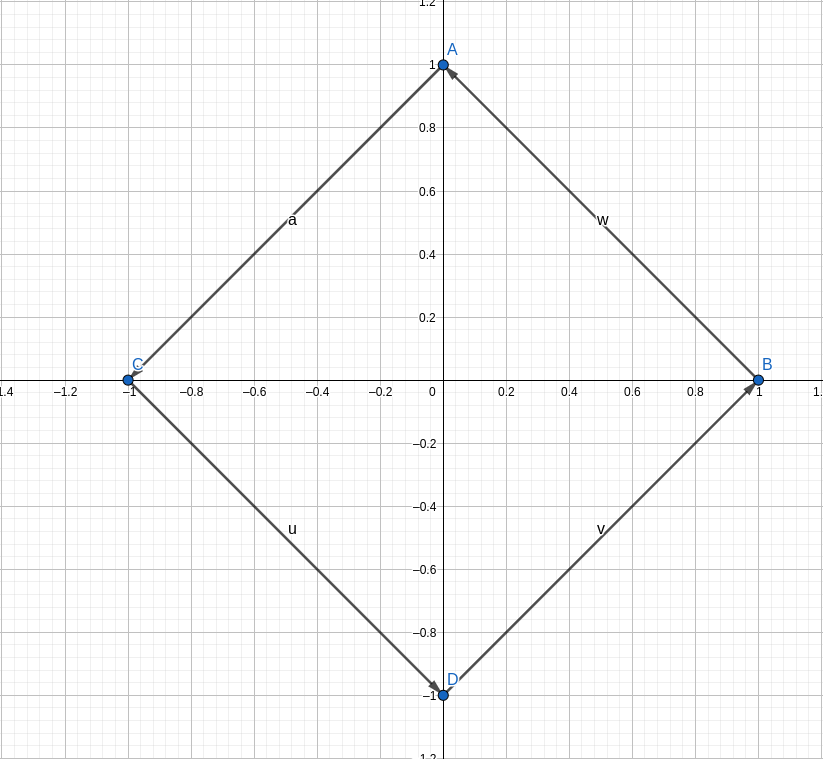
\includegraphics[scale=1,width=0.8\textwidth]{grafica_125.png}
\end{figure}

$g_j$ es precisamente el resultado de aplicar al vértice $j$ el movimiento que corresponde a $g$.

$r_j=\phi(r)(j)=(1\:2\:3\:4)(j)$

\item $G=S_n\quad X$ cualquier conjunto, con $X\neq \emptyset$. Consideremos $X^n=X\times~\overbrace{\ldots}^{n-veces}\times X$. Definimos una acción de $S_n$ sobre $X^n$ como sigue
\begin{gather*}
S_n\times X^n\longrightarrow X^n\\
(\sigma(x_1,x_2,\ldots,x_n))\longmapsto \sigma_{(x_1,x_2,\ldots,x_n)}:=(x_{\sigma^{-1}(1)},x_{\sigma^{-1}(2)},\ldots,x_{\sigma^{-1}(n)})
\end{gather*}

Veamos la propiedad 2). Sean $\sigma, \tau \in S_n$
\begin{gather*}
\sigma\tau_{(x_1,x_2,\ldots,x_n)} \overset{?}{=} \sigma(\tau_{(x_1,x_2,\ldots,x_n)}) \\
\sigma\tau_{(x_1,x_2,\ldots,x_n)}=(x_{(\sigma\tau)^{-1}(1)},x_{(\sigma\tau)^{-1}(2)},\ldots,x_{(\sigma\tau)^{-1}(n)})= \\
=(x_{\tau^{-1}\sigma^{-1}(1)},x_{\tau^{-1}\sigma^{-1}(2)},\ldots,x_{\tau^{-1}\sigma^{-1}(n)}) \\
\sigma_{(\tau_{(x_1,x_2,\ldots,x_n)})}=\sigma_{(x_{\tau^{-1}(1)},x_{\tau^{-1}(2)},\ldots,x_{\tau^{-1}(n)})}=\\
=\sigma_{(y_1,\ldots,y_n)} \qquad y_j=x_{\tau^{-1}(j)} \quad j=1,\ldots,n \\
=(y_{\sigma^{-1}(1)},y_{\sigma^{-1}(2)},\ldots,y_{\sigma^{-1}(n)})= \\
=(x_{\tau^{-1}(\sigma^{-1}(1))},x_{\tau^{-1}(\sigma^{-1}(2))},\ldots,x_{\tau^{-1}(\sigma^{-1}(n))}=\\
=(x_{\tau^{-1}\sigma^{-1}(1)},x_{\tau^{-1}\sigma^{-1}(2)},\ldots,x_{\tau^{-1}\sigma^{-1}(n)} \\
\Rightarrow \sigma\tau_{(x_1,x_2,\ldots,x_n)}=\sigma_{(\tau_{(x_1,x_2,\ldots,x_n)})}
\end{gather*}

Nótese, la aplicación
\begin{gather*}
S_n\times X^n\longrightarrow X^n\\
(\sigma(x_1,\ldots,x_n))\longmapsto (x_{\sigma(1)},\ldots,x_{\sigma(n)})
\end{gather*}

en general, no es acción (por ejemplo, compruébese para $n=3$. \\

\textbf{12-5-21}

\item Sea $G$ un grupo y $X=G$, entonces podemos definir una acción de $G$ sobre $G$ llamada, la acción por traslación y que está definida como sigue
\begin{equation*}
G\times G\longrightarrow G\qquad (g,h)\longmapsto g_h:=gh
\end{equation*}


Si $\phi:G\longrightarrow S(G)$ es la representación asociada
\begin{gather*}
Ker(\phi)=\{g\in G/\phi(g)=id_G\}=\{g\in G/\phi(g)(h)=h\quad \forall h\in G\}=\\
=\{g\in G/g_h=h\quad \forall h\in G\}=\{g\in G/gh=h\quad \forall h\in G\}=\{1\}
\end{gather*}

Es decir, esta acción es fiel.

Si $G$ finito y $|G|=n$, entonces $S(G)\overset{\sim}{=} S_n$ y como
\begin{equation*}
\phi:G\longrightarrow S(G)\overset{\sim}{=} S_n
\end{equation*}

es un monomorfismo, aplicando el primer teorema de isomorfía, deducimos que $G\overset{\sim}{=} Im(\phi)$. \\

\textbf{Teorema de Cayley:} Todo grupo finito es isomorfo a un subgrupo de permutaciones.

\item Sea $G$ un grupo y $H\leq G$ subgrupo. Entonces
\begin{gather*}
G\times G/H\longrightarrow G/H\\
(g,xH)\longmapsto g_{(xH)}:=gxH
\end{gather*}

es una acción. También
\begin{gather*}
G\times H/G\longrightarrow H/G\\
(g,Hx)\longmapsto g_{(Hx)}:=Hxg^{-1}
\end{gather*}

es una acción.

\item Sea $G$ un grupo y consideramos $X=G$. Entonces la aplicación
\begin{equation*}
G\times G\longrightarrow G\qquad (g,h)\longmapsto g_h:=ghg^{-1}
\end{equation*}

es una acción, que llamaremos la acción por conjugación de $G$ sobre si mismo
\begin{gather*}
\phi:G\longrightarrow S(G)\\
g\longmapsto \phi(g):G\longrightarrow G\\
\qquad\qquad\qquad\phi(g)(h)=g_h=ghg^{-1}
\end{gather*}

Es decir, $\phi(g)=\varphi_g$ es el automorfismo interno por el elemento $g\in G$ 
\begin{gather*}
Img(\phi)=Int(G)\leq Aut(G) \\
Ker(\phi)=\{g\in G/\varphi_g=id_G\}=\{g\in G/\varphi_g(h)=h\quad \forall x\in G\}=\\
=\{g\in G/ghg^{-1}=h\quad \forall h\in G\}=\{g\in G/gh=hg\forall h\in G\}=Z(G)
\end{gather*}

\item Sea $G$ un grupo y considremos el conjunto $X=Sub(G)$
\begin{gather*}
G\times Sub(G)\longrightarrow Sub(G)\\
(g,H)\longmapsto g_H=gHg^{-1}
\end{gather*}

es una acción. \\

Sea $G$ un grupo y $X$ un $G-conjunto$ y sea 
\begin{equation*}
G\times X\longrightarrow X \qquad (g,x)\longmapsto g_x
\end{equation*}
la acción.

Podemos definir en $X$ la siguiente relación binaria, denotada por $\sim$. Dados $x,y\in X$
\begin{equation*}
x\sim y\overset{def}{\Leftrightarrow} \exists g\in G\quad tal\:que\quad y=g_x
\end{equation*}

Esta relación binaria es una relación de equivalencia. En efecto
\begin{itemize}
\item Simétrica. Supongamos que $x\sim y\Rightarrow$
\begin{gather*}
\exists g\in G\quad tal\:que\quad y=g_x \\
y=g_x\Rightarrow g^{-1}_{(y)}=g^{-1}(g_x)\overset{2)}{=}(g^{-1}g)_x\overset{1)}{=}1_x\overset{1)}{=}x\Rightarrow y\sim x
\end{gather*}

De la misma forma se demuestra la propiedad relfexiva y transitiva.
\end{itemize}

\end{enumerate}

\textbf{Definición:} Para cada $x\in X$, definimos la órbita de $x$, que denotaremos por $\mathcal{O}(x)$, como la clase de equivalencia de $x$ por la relación de equivalencia anterior. Entonces
\begin{gather*}
\mathcal{O}(x)=\{y\in X/x\sim y\}= \\
=\{y\in X/y=g_x\quad para\quad g\in G\}=\{g_x/g\in G\}
\end{gather*}

Tenemos que 
\begin{enumerate}[1)]
\item $\mathcal{O}(x)=\mathcal{O}(y)\Leftrightarrow x\sim y\Leftrightarrow \exists g\in G \quad tal\:que\quad y=g_x$

\item $\mathcal{O}(x)\neq \mathcal{O}(y)\Leftrightarrow \mathcal{O}(x)\cap \mathcal{O}(y)=\emptyset$

\item El conjunto de todos las órbitas, es decir, $X/\sim$, es una partición de $X$
\begin{equation*}
X=\cup_{x\in X} \mathcal{O}(x) \qquad union\:finita
\end{equation*}
\end{enumerate}

Una acción diremos que es transitiva si tiene una única órbita (si $X/\sim$ es unitario). Es decir,
\begin{equation*}
\mathcal{O}(x)=\mathcal{O}(y)\quad \forall x,y\in X
\end{equation*}

o, en otros términos, si 
\begin{equation*}
\forall x,y\in X\quad \exists g\in G\quad tal\:que \quad y=g_x
\end{equation*}

\textbf{Definición:} Sea $G$ un grupo y $X$ un $G-conjunto$. Para cada $x\in X$ definimos el estabilizador de $x$ en $G$ como 
\begin{equation*}
Stab_G(x):=\{g\in G/g_x=x\}
\end{equation*}

Se verifica que $Stab_G(x)$ es un subgrupo de $G$, también llamado grupo de isotropía de $x$ en $G$. \\

\textbf{Proposición:} Sea $G$ un grupo y $X$ un $G-conjunto$. Sean $x,y\in X$, entonces
\begin{gather*}
\mathcal{O}(x)=\mathcal{O}(y)\Leftrightarrow Stab_G(x),\:Stab_G(y)\quad son\:subgrupos\:conjugados\:de\:G. \\
\end{gather*}
($H,K\leq G$, $H$ y $K$ se dicen conjugados si $\exists g\in G$ tal que $y=g_x$). \\

\textbf{Demostración:} Suponemos que $\mathcal{O}(x)=\mathcal{O}(y)\Rightarrow x\sim y\Rightarrow \exists g\in G$ tal que $y=g_x$. Veamos que $gStab_G(x)g^{-1}=Stab_G(y)$. Lo vemos por doble inclusión.

Sea $h\in Stab_G(x)\Rightarrow h_x=x$. Consideramos $ghg^{-1}$ y lo hacemos actuar sobre y
\begin{equation*}
(ghg^{-1})_y=gh(g^{-1}_{(y)})=(gh)_x=g(h_x)=g_x=y\Rightarrow ghg^{-1}\in Stab_G(y)
\end{equation*}

Tenemos que $gStab_G(x)g^{-1}\leq Stab_G(y)$. Por el mismo razonamiento y puesto que $x=g^{-1}_y$, tendremos que
\begin{equation*}
g^{-1}Stab_G(y)g\leq Stab_G(x)\Rightarrow Stab_G(y)\leq gStab_G(x)g^{-1}
\end{equation*}

Consecuentemente
\begin{equation*}
gStab_G(x)g^{-1}=Stab_G(y)
\end{equation*}

$\hfill\square$ \\

\textbf{Teorema:} Sea $G$ un grupo finito y $X$ un $G-conjunto$. Entonces para cada $x\in X$, $\mathcal{O}(x)$ es también finito, teniéndose que
\begin{equation*}
|\mathcal{O}(x)|=\left[G:Stab_G(x)\right]
\end{equation*}

En particular $|\mathcal{O}(x)|$ es un divisor de $|G|$. \\

\textbf{Demostración:}
\begin{equation*}
G/Stab_G(x)=\{gStab_G(x)/g\in G\}\overset{\lambda}{\longrightarrow} \mathcal{O}(x)=\{g_x/g\in G\}
\end{equation*}

Definimos $\lambda(gStab_G(x)):=g_x$
\begin{gather*}
gStab_G(x)=hStab_G(x)\Leftrightarrow h^{-1}g\in Stab_G(x) \\
\Leftrightarrow (h^{-1}g)_x=x\Leftrightarrow g_x=h_x
\end{gather*}

Por tanto $\lambda$ está bien definida, y además $\lambda$ es inyectiva. Obviamente, por definición, $\lambda$ es sobreyectiva, por tanto, $\lambda$ es biyectiva. Como $G/Stab_G(x)$ es finito por ser $G$ finito, entonces $\mathcal{O}(x)$ es finito y $|\mathcal{O}(x)|=\left[G:Stab_G(x)\right]$

$\hfill\square$\\

\textbf{Ejercicio 1 (Relación 6):} $X=\{1,2,3,4\}$
\begin{gather*}
S_4\times X\longrightarrow X\qquad \sigma_i:=\sigma(i)
\end{gather*}

(2)$A_4\times X\longrightarrow X\qquad \sigma_i:=\sigma(i)$

Calcula $\mathcal{O}(2)$ y $Stab_{A_4}(2)$
\begin{gather*}
\mathcal{O}(2)=\{\sigma_2/\sigma\in A_4\}=\{\sigma(2)/\sigma\in A_4\}=\{1,2,3,4\} \\
\left[A_4:Stab_{A_4}(2)\right]=|\mathcal{O}(2)|=4\Rightarrow |Stab_{A_4}(2)|=3 \\
Stab_{A_4}(2)=\{\sigma\in A_4/\sigma_2=2\}=\{\sigma\in A_4/\sigma(2)=2\}=\\
=\left\langle(1\:3\:4)\right\rangle =\{id,(1\:3\:4),(1\:4\:3)\}
\end{gather*}

(3) $K=\{id,(1\:2)(3\:4),(1\:3)(2\:4),(1\:4)(2\:3)\}$
\begin{gather*}
K\times X\longrightarrow X \qquad \sigma_i:=\sigma(i)\\
\mathcal{O}(2)=\{\sigma_2/\sigma \in K\}=\{\sigma(2)/\sigma\in K\}=\{2,1,4,3\}=X \\
\left[K:Stab_K(2)\right]=|\mathcal{O}(2)|=4\Rightarrow Stab_K(2)=\{id\}
\end{gather*}

\textbf{Definición:} Sea $G$ un grupo y $X$ un $G-conjunto$. Un elemento de $X$ diremos que es un elemento fijo por la acción si $g_x=x\quad \forall g\in G$. 

El conjunto de los elementos fijos lo denotaremos por $Fix(X)$ 
\begin{equation*}
Fix(X)=\{x\in X/g_x=x\quad \forall g\in G\}
\end{equation*}

Notemos que 
\begin{equation*}
x\in Fix(X)\Leftrightarrow \mathcal{O}(x)=\{x\}\Leftrightarrow Stab_G(x)=G
\end{equation*}

Sea $G$ un grupo finito y $X$ un $G-conjunto$ finito. El conjunto $X/\sim$ también es finito. Supongamos
\begin{equation*}
X/\sim=\{\mathcal{O}(x_1),\mathcal{O}(x_2),\ldots,\mathcal{O}(x_r)\}
\end{equation*}

Sabemos que es una partición de $X=\cup_{i=1}^r \mathcal{O}(x_i)$ unión disjunto $\Rightarrow$
\begin{gather*}
|X|=\sum_{i=1}^r |\mathcal{O}(x_i)|=|Fix(X)|+\sum_{x_i\notin Fix(X)}|\mathcal{O}(x_i)|= \\
=|Fix(X)|+\sum_{x_i\notin Fix(X)}\left[G:Stab_G(x_i)\right]
\end{gather*}

\textbf{Ejemplo:} 
\begin{enumerate}[1)]
\item Sea $G$ un grupo cualquiera, y consideramos la acción de $G$ sobre sí misma por traslación 
\begin{equation*}
G\times G\longrightarrow G \qquad g_h:=gh
\end{equation*}

Sea $h\in G$
\begin{equation*}
\mathcal{O}(h)=\{g_h/g\in G\}=\{gh/g\in G\}=G
\end{equation*}

Por tanto $\forall h,h'\in G$, si tiene que $\mathcal{O}(h)=\mathcal{O}(h')$, es decir, esta acción es transitiva
\begin{gather*}
Stab_G(h)=\{g\in G/g_h=h\}=\{g\in G/gh=h\}=\{1\} \\
Fix(G)=\{h\in G/g_h=h\quad \forall g\in G\}=\{h\in G/gh=h\quad \forall g\in G\}=\emptyset
\end{gather*}

\item Sea $G$ un grupo y consideramos la acción de $G$ sobre sí mismo por conjugación 
\begin{gather*}
G\times G\longrightarrow G \qquad g_h:=ghg^{-1} \\
h\in G\qquad \mathcal{O}(h)=\{g_h/g\in G\}=\{ghg^{-1}/g\in G\}
\end{gather*}

se llama la clase de conjugación del elemento $h$ en $G$ y se denota por $cl(h)$
\begin{equation*}
Stab_G(h)=\{g\in G/g_h=h\}=\{g\in G/ghg^{-1}=h\}=\{g\in G/gh=hg\}\leq G
\end{equation*}

se llama el centralizador de $h$ en $G$ y se denota por $C_G(h)$
\begin{gather*}
Fix(G)=\{h\in G/g_h=h\quad \forall g\in G\}=\{h\in G/ghg^{-1}=h\quad \forall g\in G\}=\\
=\{h\in G/gh=hg\quad \forall g\in G\}=Z(G)
\end{gather*}

Supongamos que $G$ es un grupo finito
\begin{equation*}
G/N=\{cl(h_1),cl(h_2),\ldots,cl(h_r)\}
\end{equation*}
\end{enumerate}

\textbf{Ejercicio 9 (Relación 6):} Describir explícitamente las clases de conjugación de $D_4$
\begin{equation*}
D_4=\left\langle r,s/r^4=1=s^2\quad sr=r^{-1}s\right\rangle=\{1,r,r^2,r^3,s,rs,r^2s,r^3s\}
\end{equation*}

\begin{itemize}
\item $cl(1)=\{1\}$ 

\item $cl(r)=\{r,r^3\}=cl(r^3)$

\item $cl(r^2)=\{r^2\}$

\item $cl(s)=\{s,r^2s\}=cl(r^2s\}$

\item $cl(rs)=\{rs,r^3s\}=cl(r^3s)$
\end{itemize}

¿Quiénes son los centralizadores de los elementos de $D_4$? $x\in D_4$
\begin{equation*}
\left[D_4:C_G(x)\right]=|cl(x)|
\end{equation*}

\textbf{17-5-21} \\

\textbf{Ejercicio 7 (Relación 6):} Demostrar que si $G$ es finito contiene un elemento $x$ que tiene exactamente 2 conjugados, entonces $G$ admite un subgrupo normal propio. \\

\textbf{Resolución:} $x\in G$ tal que $|cl(x)|=2$. En particular $x\neq 1$.

Consideramos $C_G(x)$ ($=Stab_G(x)$). Sabemos que 
\begin{equation*}
\left[G:N\right]=|cl(x)|=2\Rightarrow N\unlhdneq G
\end{equation*}

Por otro lado, como $x\in N=\{g\in G/gx=xg\}\Rightarrow N\neq 1$. Por tanto, $N$ es un grupo normal propio de $G$. Sea $G$ un grupo, y consideramos la acción
\begin{equation*}
G\times Sub(G)\longrightarrow Sub(G)\qquad g_H:=gHg^{-1}
\end{equation*}

Para $H\in Sub(G)$
\begin{gather*}
O(H)=\{g_H/g\in G\}=\{gHg^{-1}/g\in G\} \\
Stab_G(H)=\{g\in G/g_H=H\}=\{g\in G/gHg^{-1}=H\}=\\
=\{g\in G/gH=Hg\}=N_G(H) \longrightarrow Ejercicio\:33\:(Relacion\:3)
\end{gather*}

\begin{itemize}
\item $N\unlhdneq N_G(H)$

\item Si $K\leq G$ tal que $H\unlhdneq K\Rightarrow N_G(H)\leq K$
\end{itemize}

\begin{gather*}
Fix(Sub(G))=\{H\leq G/g_H=H\quad \forall g\in G\}=\{H\leq G/gHg^{-1}=H\quad \forall g\in G\}=\\
=\{H\leq G/H\quad es\:un\:subgrupo\:normal\:de\:G\}
\end{gather*}

Si $G$ es finito $\Rightarrow O(H)$ es finito, esto es, el número de conjugados de $H$ es finito. Como
\begin{equation*}
|O(H)|=\left[G:N_G(H)\right]
\end{equation*}

entonces $|O(H)|$ es un divisor de $|G|$

\subsection{p-grupos (p número primo)}
\textbf{Definición:} Sea $p$ un número primo. Un grupo finito $G$ no trivial diremos que es un p-grupo si todo elemento de $G$ tiene orden una potencia de $p$. \\

\textbf{Ejemplos:}\begin{enumerate}[1)]
\item Para cada $n\geq 1$, $C_{p^n}=\left\langle x/x^{p^n}=1\right\rangle$ es un p-grupo. Porque si $a\in C_{p^n}\Rightarrow ord(a)\mid |C_{p^n}|=p^n\Rightarrow ord(a)=p^k\quad 0\leq k\leq n$ 

\item Para cada $n\geq 2$, el producto directo
\begin{equation*}
C_p\times C_p\times \overbrace{\ldots}^{n-veces}\times C_p
\end{equation*}

es un p-grupo.

Si $(x_1,\ldots,x_n)\in G$
\begin{gather*}
ord((x_1,\ldots,x_n))=mcm(ord(x_1),\ldots,ord(x_n)) \\
ord((x_1,\ldots,x_n))=p^k\quad 0\leq k\leq 1
\end{gather*}

Así todo elemento de $G$ tiene de orden una potencia de $p$. 

\item Si $G$ es un grupo con $|G|=p^n$ para $n\geq 1$ entonces, razonando como en el ejemplo 1, $G$ es un p-grupo.
\end{enumerate}

\textbf{Teorema de Cauchy:} Sea $G$ un grupo finito. Para cada primo $p$ divisor de $|G|$ existe $x\in G$ tal que $ord(x)=p$ (entonces $\exists H=\left\langle x\right\rangle \leq G$ tal que $|H|=p$). \\

\textbf{Demostración:} Sea $|G|=n$ y $p\mid n$ con $p$ número primo. Sea $X$ definido como sigue
\begin{equation*}
X:=\{(x_1,x_2,\ldots,x_p)\in G^p/x_1x_2\ldots x_p=1\}
\end{equation*}

Como $|G|=n\Rightarrow |X|=n^{p-1}$.

Consideramos el ciclo $\sigma=(1\:2\:\ldots\:p)\in S_p$ y $H=\left\langle \sigma \right\rangle = \{1,\sigma,\sigma^2,\ldots,\sigma^{p-1}\}$. \\

Definimos una acción de $H$ sobre $X$ como sigue
\begin{gather*}
\sigma_{(x_1,\ldots,x_p)}:=(x_1,\ldots,x_p) \\
1\leq j\leq p-1\quad \sigma^j_{(x_1,\ldots,x_p)}:=(x_{j+1},\ldots,x_p,x_1,\ldots,x_j)
\end{gather*}

\textbf{Ejercicio:} Demostrar que es una acción. Sea $(x_1,\ldots,x_p)\in X$
\begin{gather*}
O((x_1,\ldots,x_p))=\{\sigma^j_{(x_1,x_2,\ldots,x_p)}/0\leq j\leq p-1\}=\\
=\{(x_1,x_2,\ldots,x_p),(x_2,\ldots,x_p,x_1),\ldots,(x_p,\ldots,x_{p-1})\}
\end{gather*}

$|O((x_1,\ldots,x_p))|$ divide a $|H|=p\Rightarrow |O(x_1,\ldots,x_p))|=1\:\,o\:\,p$. 

Los elementos con $|O(x_1,\ldots,x_p)|=1$ son precisamente $(x_1,\ldots,x_p)\in Fix(X)$
\begin{equation*}
(x_1,\ldots,x_p)\in Fix(X)\Leftrightarrow x_1=x_2=\ldots=x_p
\end{equation*}

Puesto que $(1,1,\ldots,1)\in Fix(X)$ entonces $Fix(X)\neq \emptyset$. \\

Sabemos también 
\begin{equation*}
|X|=|Fix(X)|+\sum_{(x_1,\ldots,x_p)\notin Fix(X)}|O((x_1,\ldots,x_p))|
\end{equation*}

Si $(x_1,\ldots,x_p)\notin Fix(X)\Rightarrow |O((x_1,\ldots,x_p))|=p$.

Sea $r=|Fix(X)|$ y $s=$nº de elementos $\notin Fix(X)$
\begin{equation*}
\left. \begin{array}{c}
n^{p-1}=|X|=r+ps\Rightarrow r=n^{p-1}-ps \\
p\mid n
\end{array} \right\rbrace \Rightarrow p\mid r\Rightarrow r\geq 2
\end{equation*}

Decir que $r\geq 2$ significa que $\exists (x,x,\ldots,x)\in Fix(X)$ y 

\[(x,x,\ldots,x)\neq (1,1,\ldots,1)\]

Entonces como $(x,x,\ldots,x)\in X$, por definición de $X$, $x\ldots x=x^p=~1\quad x\neq~1$. Concluimos pues $\exists x\in X$ tal que $ord(x)=p$

$\hfill\square$\\

\textbf{Corolario:} Sea $G$ un grupo finito no trivial.
\begin{equation*}
G\:es\:un\:p-grupo\Leftrightarrow |G|=p^n\quad para\:algun\quad n\geq 1
\end{equation*}

\textbf{Demostración:} $\Leftarrow)$ Ejemplo 3.

$\Rightarrow)$ Sea $|G|=m\quad (m\geq 1)$

Sea $q$ un divisor primo de $m\Rightarrow$ por el Teorema de Cauchy $\exists x\in G$ tal que $ord(x)=q$. Por otro lado, como $G$ es un p-grupo entonces $ord(x)=p^k\quad k\geq 1$. 

Consecuentemente
\begin{equation*}
q=p^k\Rightarrow k=1\quad y\quad p=q
\end{equation*}

Si el único divisor primo de $m$ es $p\Rightarrow m=p^n$ para algún $n\geq 1$. \\

\textbf{18-5-21} \\

\textbf{Teorema de Burnside:} Sea $G$ un p-grupo finito. Entonces $|Z(G)|\geq p$. En particular, $Z(G)$ no es trivial. \\

\textbf{Demostración:} Como $G$ es un p-grupo, supongamos
\begin{equation*}
|G|=p^n,\quad n\geq 1
\end{equation*}

Si $G$ es abeliano $\Rightarrow Z(G)=G$ y se tendrá el resultado. \\

Si $G$ no es abeliano, por la fórmula de las clases
\begin{equation*}
|Z(G)|=|G|=\sum_{h\notin Z(G)}|cl(h)|
\end{equation*}

Si $h\notin Z(G)\Rightarrow |cl(h)|>1$ y como $|cl(h)|=\left[G:C_G(h)\right]$, es decir,
\begin{equation*}
|cl(h)|\mid |G|=p^n,\quad entonces \quad |cl(h)|=p^k\quad k>0
\end{equation*}

Consecuentemente, $p$ es un divisor de $\sum_{h\notin Z(G)}|cl(h)|$. Como $p\mid |G|$, obtenemos que
\begin{equation*}
p\mid |Z(G)|\Rightarrow |Z(G)|\geq p
\end{equation*}

$\hfill\square$ \\

\textbf{Corolario:} Sea $p$ un número primo y $G$ un grupo con $|G|=p^2$. Entonces $G$ es abeliano. \\

\textbf{Demostración:} Por el teorema de Burnside, $|Z(G)|\geq p$. Con lo cual $|Z(G)|=p$ ó $|Z(G)|=p^2$. \\

Supongamos que $|Z(G)|=p$ entonces $\exists a\in G$ tal que $a\notin Z(G)$.
\begin{equation*}
C_G(a)\leq G\qquad C_G(a)=\{g\in G/\:ag=ga\}
\end{equation*}

Es claro que 
\begin{equation*}
Z(G)\leq C_G(a)\Rightarrow |C_G(a)|=p^2\Rightarrow C_G(a)=G\Rightarrow a\in Z(G)\downarrow
\end{equation*}

Por tanto, $|Z(G)|=p^2=|G|\Rightarrow Z(G)=G\Rightarrow G$ es abeliano.

$\hfill\square$\\

\textbf{Corolario:} Si $G$ es un p-grupo finito entonces $G$ es resoluble. \\

\textbf{Demostración:} Sea $|G|=p^n\quad n\geq 1$.

Hacemos inducción en $n$.

Si $n=1$, entonces $|G|=p\Rightarrow G\overset{\sim}{=} C_p$ y por tanto resoluble, pues todo grupo abeliano es resoluble. \\

Sea $n>1$ y el resultado cierto para todo p-grupo de orden estrictamente menor que $p^n$. Si $G$ es abeliano $\Rightarrow G$ es resoluble y lo tendríamos.

Supongamos $G$ no abeliano
\begin{equation*}
1\unlhdneq Z(G)\unlhdneq G\Rightarrow |Z(G)|=p^k\qquad 1\leq k<n
\end{equation*}

Por hipótesis de inducción, $Z(G)$ es resoluble. Por otro lado
\begin{equation*}
|G/Z(G)|=p^{n-k}\qquad 1\leq n-k<n
\end{equation*}

y entonces, por hipótesis de inducción $G/Z(G)$ es resoluble
\begin{equation*}
\left.\begin{array}{c}
Z(G)\unlhd G\quad resoluble\\
G/Z(G)\quad resoluble
\end{array}\right\rbrace \Rightarrow G\quad resoluble
\end{equation*}

\textbf{Definición:} Sea $G$ un grupo finito y $p$ un número primo. Un subgrupo $H$ de $G$ que sea p-grupo, lo llamaremos p-subgrupo de $G$. \\

\textbf{Observación:} El teorema de Cauchy nos dice que para cada primo $p$ de $|G|$ existe un $H\leq G$, $|H|=p$ y entonces un p-subgrupo. \\

\textbf{1º Teorema de Sylow:} Sea $G$ un grupo finito con $|G|=n$. Sea $p$ un número primo divisor de $n$. Entonces para cada potencia $p^i$ con $p^i\mid n$ existe $H\leq G$ tal que $|H|=p^i$. \\

\textbf{Demostración:} Hacemos inducción en $i$.

Para $i=1$, el resultado se sigue del teorema de Cauchy. \\

Sea $i>1$ y supongamos el resultado cierto para todo grupo finito con orden divisible por $p^j$, $j<i$. Veamos para $i>1$, $|G|=n$ y $p^i\mid n$ buscamos
\begin{equation*}
H\leq G\quad tal\:que \quad |H|=p^i
\end{equation*}

Hacemos inducción sobre $|G|$. Como $p^i\mid n$ el primer caso es $|G|=p^i$ y entonces basta tomar $H=G$. 

Supongamos que $|G|=n>p^i$ y el resultado cierto para todo grupo de orden estrictamente menor que $n$, y divisible por $p^i$.

\begin{enumerate}[C{a}so 1:]
\item $\exists K\leq G$ tal que $p\cancel{\mid}\left[G:K\right]$.

Como 
\begin{gather*}
\left.\begin{array}{c}
|G|=\left[G:K\right]|K| \\
p^i\mid |G|\\
p \cancel{\mid} \left[G:K\right]
\end{array} \right\rbrace \Rightarrow p^i\mid |K| \\
\left.\begin{array}{c}
p^i\mid |K| \\
K\leq G\Rightarrow |K|<|G|
\end{array} \right\rbrace \overset{hip.induccion}{\Rightarrow} \exists H\leq K\quad tal\:que\quad |H|=p^i
\end{gather*}

Claramente $H\leq G$ y se tiene el resultado. 

\item Para todo $K\leq G$, $p\mid \left[G:K\right]$

Por la fórmula de las clases
\begin{gather*}
|Z(G)|=|G|-\sum_{h\notin Z(G)}\left[G:C_G(h)\right] \\
p\mid |G| \quad y\quad p\mid \sum\left[G:C_G(h)\right]\Rightarrow p\mid |Z(G)|
\end{gather*}

Aplicamos el teorema a $Z(G)$ y entonces $\exists N\leq Z(G)$ tal que $|N|=p$. Como $N\leq Z(G)\Rightarrow N\unlhd G$.
\begin{gather*}
x\in N\Rightarrow a\cdot x=x\cdot a\quad \forall a\in G\Rightarrow axa^{-1}=x\quad \forall a\in G\\
\Rightarrow aNa^{-1}=N\quad \forall a\in G\Rightarrow N\unlhd G
\end{gather*}

Podemos pues considerar $G/N$. Como $|N|=p$ y $p^i\mid |G|\Rightarrow p^{i-1}\mid |G/N|$. Por hipótesis de inducción en la potencia de $p$, $\exists L\leq G/N$ tal que $|L|=p^{i-1}$
\begin{gather*}
L=H/N\qquad N\unlhd H\unlhd G \\
|H/N|=p^{i-1} \Rightarrow |H|=|H/N|\cdot |N|=p^{i-1}\cdot p=p^i
\end{gather*}
$\hfill\square$
\end{enumerate}

\textbf{Definición:} Sea $G$ un grupo finito, y $p$ un número primo divisor de $|G|$. Sea $p^k$ la máxima potencia de $p$ que divide a $|G|$ (es decir, $|G|=p^km,\:p\cancel{\mid}m$). Los p-subgrupos de $G$ de orden $p^k$ se llaman p-subgrupos de Sylow de $G$. \\

\textbf{Corolario:} Todo grupo $G$ tiene p-subgrupos de Sylow para cada primo divisor de $|G|$. \\

\textbf{Ejemplos:} \begin{enumerate}[1)]
\item $n\geq 2\quad y\quad C_n=\left\langle x/x^n=1\right\rangle$.

Sea $n=p_1^{t_1}p_2^{t_2}\cdot p_k^{t_k}$ la factorización de $n$ en primos.

Para cada $1\leq i\leq k$, los $p_i$-grupos de Sylow tienen orden $p_i^{t_i}$. Sólo hay uno que 
\begin{equation*}
C_{p_i^{t_i}})\left\langle x^{s_i}\right\rangle \qquad s_i=p_1^{t_1}p_2^{t_2}\cdot p_{i-1}^{t_{i-1}}p_{i+1}^{t_{i+1}}\ldots p_k^{t_k}
\end{equation*}

\item $G=A_4,\quad |A_4|=12=3\cdot 2^2$.

Los 3-subgrupos de Sylow de $A_4$ tienen orden 3 y entonces cíclicos de orden 3.
\begin{gather*}
\mathcal{P}_1=\left\langle(1\:2\:3)\right\rangle\qquad \mathcal{P}_2=\left\langle(1\:2\:4)\right\rangle \\
\mathcal{P}_3=\left\langle(1\:3\:4)\right\rangle \qquad \mathcal{P}_4=\left\langle(2\:3\:4)\right\rangle
\end{gather*}

Los 2-subgrupos de Sylow de $A_4$ tienen orden 4 y sólo tienen uno que es
\begin{equation*}
K=\{id,(1\:2)(3\:4),(1\:3)(2\:4),(1\:4)(2\:3)\}
\end{equation*}

Si $\mathcal{P}$ es un p-subgrupo de Sylow de $G$
\begin{equation*}
|G|=p^km\qquad mcd(m,p)=1
\end{equation*}

Entonces $|\mathcal{P}|=p^k$ y por tanto $\left[G:\mathcal{P}\right]=m$
\begin{equation*}
\Rightarrow mcd(|\mathcal{P}|,\left[G:\mathcal{P}\right])=1
\end{equation*}
\end{enumerate}

\textbf{19-5-21} \\

\textbf{Lema:} Sea $G$ un grupo finito y $p$ un número primo divisro de $|G|$ y $P$ un p-subgrupo de Sylow de $G$.

Sea $H\leq G$ un p-subgrupo de $G$ tal que $H\leq N_G(P)$, entonces $H\leq P$. \\

\textbf{Demostración:}

$\left.\begin{array}{c}
P\unlhd N_G(P) \\
H\leq N_G(P)
\end{array} \right.$ Aplicamos el tercer teorema de isomorfía y entonces

\begin{equation*}
H/(H\cap P)\overset{\sim}{=} (HP)/P
\end{equation*}

con lo que $\left[H:H\cap P\right]=\left[HP:P\right]=r$
\begin{equation*}
r\mid |H|\overset{H\:es\:un\:p-grupo}{\Rightarrow} r=p^t\quad t\geq 0
\end{equation*}

Consideramos $P\leq HP\leq G\Rightarrow\left[G:P\right]=\left[G:HP\right]\left[HP:P\right]=\left[G:HP\right]\cdot r$
\begin{gather*}
\left.\begin{array}{c}
\Rightarrow r\mid \left[G:P\right] \\
Como\:P\:es\:un\:p-subgrupo\:de\:Sylow\:mcd(\left[G:P\right],|P|)=1
\end{array} \right\rbrace \Rightarrow mcd(r,p)=1 \\
\left. \begin{array}{c}
mcd(r,p)=1\\
r=p^t\quad t\geq 0
\end{array} \right\rbrace \Rightarrow t=0\quad y\quad r=1
\end{gather*}

Tenemos que $1=\left[H:H\cap P\right]\Rightarrow H=H\cap P\Rightarrow H\leq P$.

$\hfill\square$\\

\textbf{2º Teorema de Sylow:} Sea $G$ un grupo finito y $p$ un número primo divisor de $|G|$. Supongamos
\begin{equation*}
|G|=p^km\quad con \quad mcd(p,m)=1
\end{equation*}

Entonces
\begin{enumerate}[(a)]
\item Todo p-subgrupo de $G$ está contenido en algún p-subgrupo de Sylow de $G$.

\item Cualesquiera dos p-subgrupos de Sylow de $G$ son conjugados (es decir, si $P_1$, $P_2$, son dos p-subgrupos de Sylow de $G$ entonces $\exists g\in G$ tal que $P_2~=~gP_2g^{-1}$).

\item Si $n_p:=$ número de p-subgrupo de Sylow de $G$, se tiene que
\begin{equation*}
n_p\mid m\quad y\quad n_p\equiv 1\mod{p}
\end{equation*}
\end{enumerate}

\textbf{Demostración:}
\begin{gather*}
S=\{P\leq G/P\quad es\:p-subgrupo\:de\:Sylow\}=\{P\leq G/|P|=p^k\} \\
S=\emptyset \quad y\quad |S|=n_p
\end{gather*}

Consideramos la acción de $G$ sobre $S$ por conjugación
\begin{gather*}
G\times S\longrightarrow S\qquad g_p:=gPg^{-1} \\
(|gPg^{-1}|=|P|=p^k\Rightarrow gPg^{-1}\in S)
\end{gather*}

Elegimos $P_1\in S$ fijo pero arbitrario
\begin{equation*}
O(P_1)=\{gP_1g^{-1}/g\in G\} \qquad Stab_G(P_1)=N_G(P_1)
\end{equation*}

Sabemos $|T|=\left[G:N_G(P_1)\right]$.

Consideramos 
\begin{equation*}
P_1\leq N_G(P_1)\leq G\Rightarrow\left[G:P_1\right]=m=\left[G:N_G(P_1)\right]\left[N_G(P_1):P_1\right]=|T|\left[N_G(P_1):P_1\right]
\end{equation*}

Por tanto $|T|\mid m\quad y\quad mcd(p,|T|)=1$
\begin{enumerate}[(a)]
\item Sea $H$ un p-subgrupo de $G$ no trivial, entonces $|H|=p^r\quad 1\leq r\leq k$. Consideramos la acción anterior de $H$ sobre $T$
\begin{gather*}
H\times T\longrightarrow T\qquad h_p:=hPh^{-1} \\
(P\in T\Rightarrow P=gP_1g^{-1}\Rightarrow hPh^{-1}=hgP_1(hg)^{-1}\Rightarrow hPh^{-1}\in T) \\
|T|=\sum_{p\in T}|\mathcal{O}(P)|=\sum_{p\in T}\left[H:Stab_H(P)\right]
\end{gather*}

Es fácil ver que $Stab_H(P)=H\cap N_G(P)$
\begin{gather*}
\left.\begin{array}{c}
H\cap N_G(P)\leq N_G(P)\quad P\:p-subgrupo\:de\:Sylow\:de\:G \\
H\cap N_G(P)\leq H\Rightarrow H\cap N_G(P)\quad es\:un\:p-subgrupo\:de\:G
\end{array}\right\rbrace\Rightarrow\\
\Rightarrow\left.\begin{array}{c}
H\cap N_G(P)\leq P\\
H\cap N_G(P)\leq H
\end{array}\right\rbrace \Rightarrow H\cap N_G(P)\leq P\cap H
\end{gather*}

y puesto que $P\cap H\leq H\cap N_G(P)$ obviamente $\Rightarrow H\cap N_G(P)=H\cap P$
\begin{gather*}
|T|=\sum_{P\in T}\left[H:H\cap P\right] \\
|T|\mid m\quad \left[H:H\cap P\right]\mid |H|=p^r\quad y\quad mcd(p,m)=1
\end{gather*}

Entonces $\exists P\in T$ tal que $\left[H:H\cap P\right]=1\Rightarrow H=H\cap P\Rightarrow H\leq P$ lo que demuestra (a).

\item Sean $P_1,\,P_2$, dos p-subgrupos de Sylow de $G$. Aplicamos (a) a $H=P_2$ y entonces $\exists P\in T=\{gP_1g^{-1}/g\in G\}$ tal que
\begin{equation*}
\left.\begin{array}{c}
P_2\leq P\\
|P_2|=p^k=|P|
\end{array}\right\rbrace \Rightarrow P_2=P
\end{equation*}

Por tanto $\exists g\in G$ tal que $P_2=gP_1g^{-1}$ que es (b).

\item Por (b), $S=T$, y entonces $n_p=|S|=|T|$ y por tanto $n_p\mid m$. Tomamos $H=P_1$ en (a) y entonces la igualdad
\begin{equation*}
|T|=\sum_{P\in T}\left[H:H\cap P\right]
\end{equation*}

se traduce en 
\begin{equation*}
n_p=\sum_{P\in S}\left[P_1:P_1\cap P\right]
\end{equation*}

Como anteriormente $\exists P\in S$ tal que
\begin{equation*}
\left[P_1:P_1\cap P\right]=1\Rightarrow P_1=P_1\cap P\Rightarrow P\leq P_1
\end{equation*}

como ambos son de Sylow $|P|=p^k=|P_1|\Rightarrow P=P_1$.

Entonces existe un único $P=P_1\in S$ tal que
\begin{equation*}
\left[P_1:P\cap P_1\right]=1
\end{equation*}

y para cualquier $P\in S$, $P\neq P_1$, necesariamente $\left[P_1:P_1\cap P\right]>1$ y entonces divisible por el número $p$.
\begin{equation*}
n_p=1+\sum_{\left.\begin{array}{c}
P\in S\\
P\neq P_1
\end{array}\right.}\left[P_1:P_1\cap P\right]\Rightarrow n_p=1+pr\Rightarrow n_p=1\mod{p}
\end{equation*}

$\hfill\square$
\end{enumerate}

\textbf{Corolario:} En las hipótesis del 2º Teorema de Sylow. Sea $P$ un p-subgrupo de Sylow de $G$
\begin{equation*}
P\unlhd G \Leftrightarrow n_p=1
\end{equation*}

\textbf{Demostración:} Como $gPg^{-1}$ es p-subgrupo de Sylow de $G$ entonces
\begin{equation*}
n_p=1\Leftrightarrow gPg^{-1}=P\qquad \forall g\in G\Leftrightarrow P\unlhd G
\end{equation*}

\textbf{Corolario:} Sea $G$ un grupo finito en el que todo sus subgrupos de Sylow son normales. Entonces $G$ es el producto directo interno de sus subgrupos de Sylow. \\

\textbf{Demostración. Ejercicio:} Sea $G$ un grupo finito, $H_1,\ldots,H_k\quad k\geq 2$, subgrupos normales de $G$ tal que $mcd(|H_i|,|H_j|)=1$. Entonces
\begin{equation*}
|H_1\ldots H_k|=|H_1|\ldots|H_k|
\end{equation*}

Supongamos que $|G|=p_1^{t_1}p_2^{t_2}\ldots p_k^{t_k}$ su factorización en número primos. Para cada $1\leq i\leq k$ sea $P_i$ el único $p_i$-subgrupo de Sylow de $G$. ($P_i\unlhd G\Rightarrow n_{p_i}=1$)

\begin{enumerate}
\item $P_i\unlhd G\qquad i=1,\ldots,k$

\item $|P_i|=p_i^{t_i}\qquad 1\leq i\leq k$
\begin{equation*}
mcd(|P_i|,|P_j|)=1\quad si\quad i\neq j
\end{equation*}

y entonces por el ejercicio anterior
\begin{equation*}
|P_1P_2\ldots P_k|=p_1^{t_1}p_2^{t_2}\ldots p_k^{t_k}=|G|\Rightarrow P_1P_2\ldots P_k=G
\end{equation*}

\item $(P_1\ldots P_{i-1})\cap P_i=1\qquad \forall i=2,\ldots,k$.

En efecto si 
\begin{equation*}
\left.\begin{array}{c}
x\in (P_1\ldots P_{i-1})\cap P_i\Rightarrow ord(x)\mid (P_1\ldots P_{i-1})=p_1^{t_1}\ldots p_{i-1}^{t_{i-1}} \\
ord(x)\mid |P_i|=p_i^{t_i}
\end{array}\right\rbrace \Rightarrow ord(x)=1\Rightarrow x=1
\end{equation*}

Consecuentemente, $G$ es el producto directo interno de $P_1,P_2,\ldots,P_k$. En otros términos
\begin{equation*}
G\overset{\sim}{=} P_1\times P_2\times \ldots \times P_k
\end{equation*}
\end{enumerate}

\textbf{Ejemplo:} Si $G$ es un grupo abeliano finito, entonces para $p$ primo divisor de $|G|$, $np=1$, puesto que todo subgrupo de $G$ es normal.

Además si $P$ es el único p-subgrupo de Sylow de $G$, este es dado por
\begin{equation*}
P=\{x\in G/ord(x)=p^i\quad 0\leq i\leq k\}
\end{equation*}

siendo $p^k$ la máxima potencia de $p$ que divide a $|G|$ (Ejercicio). $P$ se llama la componente p-primaria de $G$. \\

\textbf{Ejercicio 5 (Relación 5):} Hallar todos los subgrupos de Sylow de $S_3$ y $S_4$
\begin{equation*}
|S_3|=6=2\cdot 3
\end{equation*}

Los 2-subgrupos de Sylow de $S_3$ tienen orden 2, y entonces son
\begin{equation*}
\left\langle (1\:2)\right\rangle,\quad\left\langle(1\:3)\right\rangle,\quad\left\langle(2\:3)\right\rangle
\end{equation*}

Los 3-subgrupos de Sylow de $S_3$ tienen orden 3 y sólo hay 1
\begin{equation*}
A_3=\left\langle(1\:2\:3)\right\rangle=\{id,(1\:2\:3),(1\:3\:2)\}
\end{equation*}

$S_4\qquad |S_4|=24=3\cdot 2^3$

Los 3-subgrupos de Sylow de $S_4$ tienen orden 3 y entonces son 
\begin{equation*}
P_1=\left\langle(1\:2\:3)\right\rangle,\quad P_2=\left\langle(1\:2\:4)\right\rangle,\quad P_3=\left\langle(1\:3\:4)\right\rangle,\quad P_4=\left\langle(2\:3\:4)\right\rangle
\end{equation*}

Los 2-subgrupos de Sylow de $S_4$ tienen orden
\begin{equation*}
2^3=8\qquad n_2=nº\:de\:subgrupos\:de\:Sylow\:de\:G
\end{equation*}

Por el 2º Teorema de Sylow
\begin{equation*}
n_2\mid 3 \quad y\quad n_2\equiv 1\mod{2}\Rightarrow n_2=1\:\,o\:\,n_2=3
\end{equation*}

Si $n_2=1$ entonces $\exists!P\leq S_4$ con $|P|=8$. Sea $(i\:j)\in S_4$ cualquier trasposición y $H=\left\langle(i\:j)\right\rangle$.

Como $|H|=2$ es un 2-subgrupo de $S_4$ entonces por (a) del 2º Teorema de Sylow, $H\leq P$. Con lo que $(i\:j)\in P\quad \forall (i\:j)\in S_4\Rightarrow S_4\leq P$, pues las trasposiciones generan $S_4\downarrow$. \\

Por tanto $n_2=3$. Sean $Q_1,Q_2,Q_3$ los 2-subgrupos de Sylow de $S_4$
\begin{equation*}
|Q_i|=8\qquad i=1,2,3
\end{equation*}

Por tanto $i=1,2,3$
\begin{equation*}
K=\{id,(1\:2)(3\:4),(1\:3)(2\:4),(1\:4)(2\:3)\}\leq Q_i
\end{equation*}

En efecto puesto que $|K|=4=2^2$, $K$ es un 2-subgrupo de $S_4$ y entonces por (a) del 2º Teorema de Sylow
\begin{equation*}
\exists i\quad tal\:que\quad K\leq Q_i
\end{equation*}

Supongamos $i=1$, es decir, $K\leq Q_1$. Por (b) del 2º Teorema de Sylow $\exists \sigma,\gamma\in S_4$ tal que
\begin{equation*}
Q_2=\sigma Q_1\sigma^{-1},\qquad Q_3=\gamma Q_1\gamma^{-1}
\end{equation*}

Sabemos que $K\unlhd S_4$
\begin{equation*}
K\leq Q_1\overset{K\unlhd S_4}{\Rightarrow} \left.\begin{array}{c}
K=\sigma K\sigma^{-1}\leq \sigma Q_1\sigma^{-1}=Q_2\\
K=\gamma K\gamma^{-1}\leq \gamma Q_1\gamma^{-1}=Q_3
\end{array}\right.
\end{equation*}

Tenemos pues determinado cuatro elementos en cada $Q_i$. Para buscar los otros cuatro, razonamos como sigue. Sea $\tau\in S_4$ una trasposición. Aplicamos el 3º Teorema de isomorfía
\begin{equation*}
\left.\begin{array}{c}
K\unlhd S_4\\
H=\left\langle\tau\right\rangle \leq S_4
\end{array}\right\rbrace \Rightarrow H/(K\cap H)\overset{\sim}{=} (KH)/K
\end{equation*}

Como
\begin{gather*}
\left.\begin{array}{c}
K\cap H=\{id\} \\
H=\{id,\tau\}
\end{array}\right.,\quad entonces \quad H\overset{\sim}{=} (KH)/K \\
|(KH)/K|=|H|\Rightarrow |KH|=|K||H|=4\cdot 2=8
\end{gather*}

Por tanto, multiplicamos $K$ por $\left\langle\tau\right\rangle$ y obtenemos los 2-subgrupos de Sylow
\begin{gather*}
Q_1=K\left\langle(1\:2)\right\rangle=\{id,(1\:2)(3\:4),(1\:3)(2\:4),(1\:4)(2\:3),\\
,(1\:2),(3\:4),(1\:3\:2\:4),(1\:4\:2\:3)\} \\
Q_2=K\left\langle(1\:3)\right\rangle=\{id,(1\:2)(3\:4),(1\:3)(2\:4),(1\:4)(2\:3),\\
,(1\:3),(2\:4),(1\:2\:3\:4),(1\:4\:3\:2)\} \\
Q_3=K\left\langle(1\:4)\right\rangle=\{id,(1\:2)(3\:4),(1\:3)(2\:4),(1\:4)(2\:3),\\
,(1\:4),(2\:3),(1\:2\:4\:3),(1\:3\:4\:2)\} 
\end{gather*}

\textbf{Ejercicio 21 (Relación 5):} Demostrar que $D_4$ es isomorfo a los 2-subgrupos de Sylow de $S_4$. \\
\textbf{Pista:} Considerar la representación asociada a la acción de $D_4$ sobre los vértices del cuadrado
\begin{gather*}
D_4=\left\langle r,s/r^4=1=s^2,\quad sr=r^{-1}s\right\rangle \\
\phi:D_4\longrightarrow S_4 \qquad \left.\begin{array}{c}
\phi(r^i)=(1\:2\:3\:4)^i\qquad 0\leq i\leq 3 \\
\phi(r^is)=(1\:2\:3\:4)^i(2\:4)\qquad 0\leq i\leq 3
\end{array} \right.
\end{gather*}

$\phi$ es un monomorfismo
\begin{equation*}
D_4/Ker(\phi)\overset{\sim}{=} Img(\phi)
\end{equation*}

Como $Ker(\phi)=1$, $D_4\overset{\sim}{=} Img(\phi)\Rightarrow |D_4|=|Img(\phi)|$. $Img(\phi)$ es un 2-subgrupo de Sylow de $S_4$ (concretamente, $Img(\phi)=Q_2$) 
\begin{equation*}
D_4\overset{\sim}{=} Q_2\quad y\:entonces\:como \quad \left.\begin{array}{c}
Q_2\overset{\sim}{=} Q_1\\
Q_2\overset{\sim}{=} Q_3
\end{array} \right.
\end{equation*}

Se concluye el ejercicio. \\

\textbf{24-5-21} \\

\textbf{Ejercicio 23 (Relación 5):} $G$ con $|G|=12$ y con $n_3>1$. Demostrar que $G\overset{\sim}{=}A_4$.

$|G|=12=3\cdot 2^2$

Sea $\mathcal{P}$ un 3-subgrupo de Sylow de $G$, $|\mathcal{P}|=3$, y $\mathcal{P}$ es un subgrupo no normal en $G$ (pues $n_3>1$).

Se considera $G/\mathcal{P}=\{x\mathcal{P}/x\in G\}$ conjunto, y se considera la acción por traslación
\begin{equation*}
G\times G/\mathcal{P}\longrightarrow G/\mathcal{P} \qquad g_{(x\mathcal{P})}=(gx)\mathcal{P}
\end{equation*}

Consideramos la representación asociada
\begin{gather*}
\phi:G\longrightarrow S(G/\mathcal{P})\quad homomorfismo\\
g\longmapsto \left.\begin{array}{c}
\phi(g)\\
\phi(g)(x\mathcal{P})=g_{x\mathcal{P}}=(gx)\mathcal{P}
\end{array} \right. \\
Ker(\phi)=\{g\in G/\phi(g)=id_{G/\mathcal{P}}\}=\{g\in G/\phi(g)(x\mathcal{P})=x\mathcal{P}\quad \forall x\in G\}= \\
=\{g\in G/g_{x\mathcal{P}}=x\mathcal{P}\quad \forall x\in G\}=\{g\in G/(gx)\mathcal{P}=x\mathcal{P}\quad \forall x\in G\}
\end{gather*}

Veamos $Ker(\phi)\leq \mathcal{P}$. Sea $g\in Ker(\phi)\Rightarrow (gx)\mathcal{P}=x\mathcal{P} \quad \forall x\in G$. En particular, considerando $x=1$, será 
\begin{equation*}
g\mathcal{P}=\mathcal{P}\Rightarrow g\in \mathcal{P}
\end{equation*}

Por tanto
\begin{equation*}
\left.\begin{array}{c}
Ker(\phi)\leq \mathcal{P} \\
|\mathcal{P}|=3
\end{array} \right\rbrace\Rightarrow \left\lbrace \begin{array}{c}
Ker(\phi)=\{1\} \\
Ker(\phi)=\mathcal{P}
\end{array}\right.
\end{equation*}

Como $Ker(\phi)\unlhd G$ y $\mathcal{P}\cancel{\unlhd} G\Rightarrow Ker(\phi)\neq \mathcal{P}$. Entonces $Ker(\phi)=\{1\}$
\begin{gather*}
\phi:G\longrightarrow S(G/\mathcal{P}) \quad es\:monomorfismo\Rightarrow G\overset{\sim}{=} Img(\phi) \\
|G/X|=\left[G:\mathcal{P}\right]=\frac{|G|}{|\mathcal{P}|}=\frac{12}{3}=4 \Rightarrow S(G/\mathcal{P})\overset{\sim}{=} S_4
\end{gather*}

$Img(\phi)$ es isomorfo a un subgrupo de $S_4$ de orden 12 y entonces $Img(\phi)\overset{\sim}{=} A_4$. Considerando ambos isomorfismos obtenemos
\begin{equation*}
G\overset{\sim}{=} A_4
\end{equation*}

\textbf{Ejercicio 26 (Relación 5):}\begin{enumerate}[1)]
\item Demostrar que no existen grupos simples de orden 28.

\item Demostrar que todo grupo de orden 28 es resoluble.
\end{enumerate}

\textbf{Resolución:} $G$ con $|G|=28=7\cdot 2^2$
\begin{equation*}
n_7\mid 4\quad y \quad n_7\equiv 1\mod{7} \Rightarrow n_7=1
\end{equation*}

Si $n_7=1\Rightarrow \exists\mathcal{P}\unlhd G$ tal que $|\mathcal{P}|=7$. En particular $G$ no es simple. \\

2) $\left. \begin{array}{c}
\mathcal{P}\unlhd G\quad y\quad |\mathcal{P}|=7\Rightarrow \mathcal{P} \quad es\:resoluble\\
|G/\mathcal{P}|=4\Rightarrow G/\mathcal{P}\quad es\:un\:2-grupo\Rightarrow G/\mathcal{P}\quad resoluble
\end{array} \right\rbrace \Rightarrow G\quad resoluble$ \\

\textbf{Ejercicio 25 (Relación 5):} \begin{enumerate}[1)]
\item Demostrar que todo grupo de orden 12 admite un subgrupo normal de orden 3 o un subgrupo normal de orden 4. En particular, no es simple. 

\item Demostrar que todo grupo de orden 12 es resoluble.
\end{enumerate}

\textbf{Resolución:} $G$ con $|G|=12=3\cdot 2^2$
\begin{equation*}
n_3\mid 4\quad y\quad n_3\equiv 1\mod{3} \Rightarrow n_3=1\quad o\quad n_3=4
\end{equation*}

Si $n_3=1\quad \exists!\mathcal{P}\unlhd G$ tal que $|\mathcal{P}|=3$ estaría hecho.

Si $n_3=4$ veamos que $n_2=1$.

Sean $\mathcal{P}_1,\mathcal{P}_2,\mathcal{P}_3,\mathcal{P}_4$ los 3-subgrupos de Sylow de $G$
\begin{equation*}
\mathcal{P_i}\neq \mathcal{P}_j \quad \forall i\neq j\qquad |\mathcal{P}_i|=3\quad \forall i=1,2,3,4
\end{equation*}

Se tiene además que $\mathcal{P}_i\cap \mathcal{P}_j=\{1\}\quad \forall i\neq j$ porque
\begin{equation*}
\left.\begin{array}{c}
\mathcal{P}_i\cap \mathcal{P}_j\leq \mathcal{P}_i\\
|\mathcal{P}_i|=3
\end{array}\right\rbrace \Rightarrow \left\lbrace \begin{array}{c}
\mathcal{P}_i\cap \mathcal{P}_j=\{1\}\\
\mathcal{P}_i\cap \mathcal{P}_j=\mathcal{P}_i\Rightarrow\mathcal{P}_j\leq \mathcal{P}_i\Rightarrow \mathcal{P}_j=\mathcal{P}_i \downarrow
\end{array} \right.
\end{equation*}

Luego $\mathcal{P}_i\cap \mathcal{P}_j=\{1\}$. Todos los elementos de cada $\mathcal{P}_i$ no triviales tienen orden 3, para cada $i=1,2,3,4$. 

Consideramos el conjunto
\begin{equation*}
\cup_{i=1}^4 \mathcal{P}_i-\{1\}
\end{equation*}

dicho conjunto tiene exactamente 8 elementos, todos ellos de orden 3. De hecho en dicho conjunto están todos los elementos del grupo $G$ de orden 3. 

Nos quedan entonces $12-8=4$ elementos de $G$ cuyo orden es 3. Como ha de existir un 2-grupo de Sylow $Q\unlhd G$ y entonces
\begin{equation*}
\exists Q\leq G\quad con\quad |Q|=4
\end{equation*}

Combinando ambos hechos $\exists! Q\unlhd G$ con $|Q|=4$, es decir, $n_2=1$. \\

2) $|G|=12\Rightarrow G$ resoluble.

Por (1) $\exists \mathcal{P}\unlhd G$ con $|\mathcal{P}|=3$ ó $\exists Q\unlhd G$ con $|Q|=4$.

En el primer caso
\begin{equation*}
\left. \begin{array}{c}
\mathcal{P}\unlhd G\quad |\mathcal{P}|=3\Rightarrow \mathcal{P}\quad resoluble \\
|G/\mathcal{P}|=4\Rightarrow G/\mathcal{P}\quad es\:un\:2-grupo \Rightarrow G/\mathcal{P}\quad resoluble
\end{array} \right\rbrace \Rightarrow G\quad resoluble
\end{equation*}

En el segundo caso
\begin{equation*}
\left.\begin{array}{c}
Q\unlhd G\quad con\quad |Q|=4\Rightarrow Q\quad resoluble\\
|G/Q|=3\Rightarrow G/Q\quad resoluble
\end{array} \right\rbrace \Rightarrow G\quad resoluble
\end{equation*}

\textbf{Ejercicio 30 (Relación 5):} Demostrar que todo grupo de orden 24 es resoluble. Sea $G$ con
\begin{gather*}
|G|=24=8\cdot 3=2^3\cdot 3 \\
n_3\mid 8 \quad y\quad n_3\equiv 1\mod{3}\Rightarrow n_3=1\quad o\quad n_3=4
\end{gather*}

Si $n_3=1\Rightarrow \exists!\mathcal{P}\unlhd G$ con $|\mathcal{P}|=3$ y por tanto resoluble. 

Como $|G/\mathcal{P}|=8=2^3\Rightarrow$ es un 2-grupo, luego es resoluble $\Rightarrow$ concluimos pues que $G$ es resoluble. \\

Si $n_3=4$. Sean $\mathcal{P}_1,\mathcal{P}_2,\mathcal{P}_3,\mathcal{P}_4$ los 3-subgrupos de Sylow
\begin{equation*}
\left.\begin{array}{c}
|\mathcal{P}_i|=3\qquad \forall i=1,2,3,4\\
\mathcal{P}_i\cap \mathcal{P}_j=\{1\}\qquad \forall i\neq j
\end{array} \right.
\end{equation*}

Sea $X=\{\mathcal{P}_1,\mathcal{P}_2,\mathcal{P}_3,\mathcal{P}_4\}$ y 
\begin{equation*}
G\times X\longrightarrow X\qquad g_{\mathcal{P}_i}=g\mathcal{P}_ig^{-1}\quad \forall i=1,2,3,4
\end{equation*}

La representación asociada es un homomorfismo
\begin{gather*}
\phi:G\longrightarrow S(X)\overset{\sim}{=} S_4 \\
Ker(\phi)=\{g/\phi(g)=Id_X\}=\{g\in G/\phi(g)(\mathcal{P}_i)=\mathcal{P}_i\quad \forall i=1,2,3,4\}=\\
=\{g\in G/g\mathcal{P}_ig^{-1}=\mathcal{P}_i\quad \forall i=1,2,3,4\}
\end{gather*}

Como $\mathcal{P}_i$ no es normal en $G$ ($n_3=4>1$) entonces 
\begin{equation*}
\left.\begin{array}{c}
Ker(\phi)\unlhdneq G\\
|G|=24
\end{array} \right\rbrace \Rightarrow |Ker(\phi)|\in\{1,2,3,4,6,8,12\}
\end{equation*}

$\Rightarrow Ker(\phi)$ es resoluble.
\begin{equation*}
G/Ker(\phi)\overset{\sim}{=} Img(\phi)\leq S_4
\end{equation*}

$S_4$ resoluble $\Rightarrow Img(\phi)$ es resoluble (pues todo subgrupo de un grupo resolubles es resoluble). \\

\textbf{25-5-21} \\

\textbf{Ejercicio 32 (Relación 5):} Si $G$ es un grupo de orden 30 entonces $n_3=1$ ó $n_5=1$. Concluir que $G$ es resoluble.
\begin{gather*}
|G|=30=2\cdot 3\cdot 5\\
n_3\mid 10 \quad y\quad n_3\equiv 1\mod{3}\Rightarrow n_3=1\quad o\quad n_3=10 \\
n_5\mid 6 \quad y\quad n_5\equiv 1\mod{5}\Rightarrow n_5=1\quad o\quad n_5=6
\end{gather*}

Supongamos que $n_3>1$ y $n_5>1$.

Si $n_3>1\Rightarrow n_3=10$. Sean $\{\mathcal{P}_i\}_{i=1,\ldots,10}$ los 3-subgrupos de Sylow. Como $|\mathcal{P}_i|=3\quad \forall i$, entonces $\mathcal{P}_i\cap \mathcal{P}_j=\{1\}\quad \forall i\neq j$. 

Por tanto en $\cup_{i=1}^{10}\mathcal{P}_i-\{1\}$ hay 20 elementos de orden 3. \\

Si $n_5>1\Rightarrow n_5=6$. Sea $\{\mathcal{Q}_j\}_{j=1,\ldots,5}$ los 5-subgrupos de Sylow. Como $|\mathcal{Q}_i|=5\quad \forall i$, entonces $\mathcal{Q}_j\cap \mathcal{Q}_r=\{1\}\quad \forall j\neq r$.

Por tanto, en $\cup_{j=1}^6 \mathcal{Q}_j-\{1\}$ hay 24 elementos de orden 5. Entonces 
\begin{equation*}
|G|\geq 20+24=44\downarrow
\end{equation*}

$n_3=1\quad o\quad n_5=1$.
Si $n_3=1\Rightarrow \exists!\mathcal{P}\unlhd G$ con $|\mathcal{P}|=3$ (resoluble)
\begin{equation*}
|G/\mathcal{P}|=10\quad (resoluble)\Rightarrow G\quad resoluble
\end{equation*}

Si $n_5=1\Rightarrow \exists! \mathcal{Q}\unlhd G$ con $|\mathcal{Q}|=5$ (resoluble)
\begin{equation*}
|G/\mathcal{Q}|=6\quad (resoluble)\Rightarrow G\quad (resoluble)
\end{equation*}

\textbf{Ejercicios 35, 36 y 37 (Relación 5):}
\begin{enumerate}[(a)]
\item Demostrar que todo grupo de orden $p\cdot q$, con $p$ y $q$ primos distintos, es resoluble
\begin{equation*}
|G|=pq\quad supongamos\quad p>q
\end{equation*}

Sabemos que 
\begin{equation*}
n_p\mid q\quad y\quad n_p\equiv 1\mod{p} \Rightarrow n_p=1
\end{equation*}

Si $n_p=q$ entonces $q\equiv 1 \mod{p}$, es decir,
\begin{equation*}
q=1+kp\quad en\:contradiccion\:con\:que\quad p>q
\end{equation*}

Por tanto $n_p=1$ y con ello se deduce que $G$ es resoluble.

\item Si $|G|=p^2q$ con $p$ y $q$ primos distintos $G$ es resoluble.
	\begin{enumerate}[\bfseries C{a}so 1:]
	\item $p>q$ entonces razonando como en (a) $n_p=1$ y $G$ es resoluble.
	
	\item $p<q$
	\begin{equation*}
	n_q\mid p^2\quad y\quad n_q\equiv 1 \mod{q}
	\end{equation*}
	
	$n_q\neq p$ pues $p<q$. Luego $n_q=1\quad o\quad n_q=p^2$.
	
	Si $n_q=1\Rightarrow \exists!\mathcal{Q}\unlhd G \quad |\mathcal{Q}|=q$ y por lo tanto resoluble. Como $|G/\mathcal{Q}|=p^2$ (resoluble por ser un p-grupo) $\Rightarrow G$ es resoluble. \\
	
	Si $n_q=p^2$, sea $\{\mathcal{P}_i\}_{i=1,\ldots,p^2}$ los q-subgrupos de Sylow de $G$.
	\begin{equation*}
	|\mathcal{P}_i|=q\quad \forall i\quad y\:entonces\quad \mathcal{P}_i\cap \mathcal{P}_j=\{1\}
	\end{equation*}	
	
	Entonces en $\cup_{i=1}^{p^2} \mathcal{P}_i -\{1\}$ hay $p^2(q-1)$ elementos de orden $q$. Como $|G|=p^2q$, nos quedan
	\begin{equation*}
	p^2q-p^2(q-1)=p^2
	\end{equation*}	
	
	en el grupo de $G$, que son los que forman el único p-subgrupo de Sylow de $G$. 
	
	Así $n_p=1\Rightarrow G$ es resoluble. 
	\end{enumerate}

\item Demostrar que si $|G|=p_1p_2p_3$, $p_1,\,p_2,\,p_3$ primos distintos tales que $p_3>p_1p_2$, en ese caso $G$ es resoluble
\begin{equation*}
n_{p_3}\mid p_1p_2\quad y\quad n_{p_3}\equiv 1\mod{p_3}
\end{equation*}

Veamos que necesariamente $n_{p_3}=1$.
\begin{gather*}
Si\quad n_{p_3}=p_1\Rightarrow p_1\equiv 1\mod{p_3} \Rightarrow p_1=1+kp_3 \\
\Rightarrow p_1p_2=p_2+kp_3p_2\Rightarrow p_1p_2>p_3\downarrow
\end{gather*}

De la misma forma se demuestra $n_{p_3}\neq p_2$. 
\begin{gather*}
Si\quad n_{p_3}=p_1p_2 \Rightarrow p_1p_2\equiv 1\mod{p_3}\Rightarrow p_1p_2=1+tp_3 \Rightarrow p_1p_2>p_3\downarrow \\
Si\quad n_{p_3}=1\Rightarrow \exists!\mathcal{Q}\unlhd G\quad tal\:que\quad |\mathcal{Q}|=p_3 \quad como \quad |G/\mathcal{Q}|=p_1p_2\Rightarrow \\
\overset{(a)}{\Rightarrow} |G/\mathcal{Q}|\quad resoluble \Rightarrow G\quad resoluble
\end{gather*}
\end{enumerate}

\textbf{Ejercicio 4 (Relación 5):} Sea $G$ un p-grupo y $X$ un G-conjunto finito. Demostrar que $|X|=|Fix(X)|\mod{p}$ \\

Supongamos que $X/\sim=\{O(x_1),\ldots,O(x_n)\}$
\begin{gather*}
|X|=|Fix(X)|+\sum_{x_i\notin Fix(X)}|O(x_i)|=|Fix(X)|+\sum_{x_i\notin Fix(X)} \left[G:Stab_G(x_i)\right] \\
x_i\notin Fix(X)\Leftrightarrow |O(x_i)|>1\Leftrightarrow \left[G:Stab_G(x_i)\right]>1 \\
\left[G:Stab_G(x_i)\right]\mid |G|=p^k \quad k\geq 1\Rightarrow \left[G:Stab_G(x_i)\right]=p^r\quad 0<r\leq k
\end{gather*}

Por tanto, $p\mid \sum_{x_i\notin Fix(X)}\left[G:Stab_G(x_i)\right]$
\begin{gather*}
|X|=|Fix(X)|+ps\quad s\in\mathbb{N}\Rightarrow |X|=|Fix(X)|\mod{p}
\end{gather*}

\textbf{Ejercicio 11 (Relación 5):} Un subgrupo $G\leq S_n$ se dice transitivo si la acción de $G$ sobre $X=\{1,2,\ldots,n\}$ es transitiva.
\begin{gather*}
S_n\times \{1,2,\ldots,n\}\longrightarrow \{1,2,\ldots,n\} \\
\sigma_i:=\sigma(i)
\end{gather*}

$G\leq S_n$, podemos considerar la acción de $G$ sobre $X$ por restricción de la anterior
\begin{equation*}
G\times X\longrightarrow X\qquad \sigma_i:=\sigma(i)\quad \left.\begin{array}{c}
\forall \sigma \in G\\
\forall i\in X
\end{array} \right.
\end{equation*}

Decir que dicha acción es transitiva es decir que tiene una única órbita. En otros términos
\begin{gather*}
O(i)=O(j)=X\qquad \forall i,j\in X \\
O(i)=\{\sigma_i/\sigma \in G\}=\{\sigma(i)/\sigma\in G\}
\end{gather*}

Entonces, decir que $G$ es transitiva es equivalente a decir que
\begin{equation*}
``para\:cualesquiera\quad i,j\in X=\{1,2,\ldots,n\},\quad \exists\sigma \in G\quad tal\:que\quad \sigma(i)=j''
\end{equation*}

Encontrar los subgrupos transitivos de $S_3$ y $S_4$.

\begin{center}
\begin{tikzpicture}[scale=0.2]
\tikzstyle{every node}+=[inner sep=0pt]
\draw [black] (37.6,-9.3) circle (3);
\draw (37.6,-9.3) node {$S_3$};
\draw [black] (13.4,-26.7) circle (3);
\draw (13.4,-26.7) node {$A_3$};
\draw [black] (30.6,-26) circle (3);
\draw (30.6,-26) node {$\left\langle(1\mbox{ }2)\right\rangle$};
\draw [black] (44,-25.8) circle (3);
\draw (44,-25.8) node {$\left\langle(1\mbox{ }3)\right\rangle$};
\draw [black] (61.4,-25.1) circle (3);
\draw (61.4,-25.1) node {$\left\langle(2\mbox{ }3)\right\rangle$};
\draw [black] (37.6,-46.2) circle (3);
\draw (37.6,-46.2) node {$\{id\}$};
\draw [black] (35.26,-44.32) -- (15.74,-28.58);
\fill [black] (15.74,-28.58) -- (16.05,-29.47) -- (16.67,-28.69);
\draw [black] (36.62,-43.37) -- (31.58,-28.83);
\fill [black] (31.58,-28.83) -- (31.37,-29.75) -- (32.32,-29.43);
\draw [black] (38.5,-43.34) -- (43.1,-28.66);
\fill [black] (43.1,-28.66) -- (42.39,-29.28) -- (43.34,-29.58);
\draw [black] (39.84,-44.21) -- (59.16,-27.09);
\fill [black] (59.16,-27.09) -- (58.22,-27.25) -- (58.89,-28);
\draw [black] (58.9,-23.44) -- (40.1,-10.96);
\fill [black] (40.1,-10.96) -- (40.49,-11.82) -- (41.04,-10.99);
\draw [black] (42.92,-23) -- (38.68,-12.1);
\fill [black] (38.68,-12.1) -- (38.51,-13.02) -- (39.44,-12.66);
\draw [black] (31.76,-23.23) -- (36.44,-12.07);
\fill [black] (36.44,-12.07) -- (35.67,-12.61) -- (36.59,-13);
\draw [black] (15.84,-24.95) -- (35.16,-11.05);
\fill [black] (35.16,-11.05) -- (34.22,-11.11) -- (34.81,-11.92);
\end{tikzpicture}
\end{center}

$S_3\leq S_3$ transitivo claramente.

$A_3=\{id,(1\:2\:3),(1\:3\:2)\}$ también transitivo.
\begin{gather*}
O(1)=\{\sigma_1/\sigma\in A_3\}=\{\sigma(1)/\sigma\in A_3\}=\{1,2,3\}=O(2)=O(3) \\
\left\langle(1\:2)\right\rangle=\{id,(1\:2)\}\quad no\:es\:transitiva \\
O(1)=\{\sigma(1)/\sigma \in \left\langle(1\:2)\right\rangle\}=\{1,2\}=O(2)\\
O(3)=\{\sigma(3)/\sigma \in \left\langle(1\:2)\right\rangle\}=\{3\}
\end{gather*}

De la misma forma se ve que $\left\langle(1\:2)\right\rangle,\:\left\langle(2\:3)\right\rangle$ tampoco son transitivas. \\

\textbf{26-5-21} \\

\textbf{Ejercicio 12 (Relación 5):} Sea $G$ un grupo finito y $H\leq G$ subgrupo tal que $\left[G:H\right]=p$ siendo $p$ el menor primo que divide al orden de $G$. Demuestre que $H\unlhd G$.

\begin{enumerate}[1)]
\item $G/H=\{xH/x\in G\}$
\begin{gather*}
G\times G/H\longrightarrow G/H\qquad g_{(xH)}:=(gx)H \\
\rho:G\longrightarrow S(G/H) \quad la\:representacion\:asociada.
\end{gather*}

Veamos que $Ker(\rho)\leq H$
\begin{gather*}
Ker(\rho)=\{g\in G/\rho(g):=id_{G/H}\}=\{g\in G/\rho(g)(xH)=xH\quad \forall x\in G\}=\\
=\{g\in G/(gx)H=xH\quad \forall x\in G\}
\end{gather*}

Si $g\in Ker(\rho)\Rightarrow (gx)H=xH\quad \forall x$.

En particular, para $x=1$
\begin{equation*}
gH=H\Rightarrow g\in H
\end{equation*}

\item Probar $\left[G:Ker(\rho)\right]\mid p!$

Por el 1º Teorema de isomorfía tenemos que
\begin{gather*}
G/Ker(\rho)\overset{\sim}{=} Img(\rho) \qquad \left[G:Ker(\rho)\right]=|Img(\rho)| \\
\left.\begin{array}{c}
Img(\rho)\leq S(G/H)\overset{\sim}{=} S_p \\
|G/H|=\left[G:H\right]=p
\end{array} \right\rbrace \Rightarrow |Img(\rho)| \mid p!
\end{gather*}

Consecuentemente $\left[G:Ker(\rho)\right] \mid p!$

\item $Ker(\rho)\leq H$

Probar que $\left[H:Ker(\rho)\right] \mid (p-1)!$. Consideramos
\begin{equation*}
Ker(\rho)\leq H\leq G\Rightarrow \left[G:Ker(\rho)\right] = \left[G:H\right]\left[H:Ker(\rho)\right]
\end{equation*}

Como $\left[G:Ker(\rho)\right]\mid p!$ por 2)$\Rightarrow$
\begin{gather*}
\Rightarrow p!=\left[G:Ker(\rho)\right]k\qquad k\in \mathcal{Z} \Rightarrow \\
\Rightarrow p!=p\cdot \left[H:Ker(\rho)\right]\cdot k\Rightarrow (p-1)!=\left[H:Ker(\rho)\right]k\Rightarrow \\
\Rightarrow \left[H:Ker(\rho)\right] \mid (p-1)!
\end{gather*}

\item Concluid que $\left[H:Ker(\rho)\right]=1$

Si no fuera 1, elegimos un primo $q$ tal que $q\mid \left[H:Ker(\rho)\right]$
\begin{equation*}
\left[H:Ker(\rho)\right] \mid |H|\Rightarrow q\mid |H| \Rightarrow q\mid |G|
\end{equation*}

Como, por el apartado 3)
\begin{equation*}
\left[H:Ker(\rho)\right]\mid (p-1)!
\end{equation*}

por transitividad
\begin{equation*}
\left.\begin{array}{c}
\left[H:Ker(\rho)\right]\mid (p-1)!\\
q\mid \left[H:Ker(\rho)\right]
\end{array} \right\rbrace \Rightarrow q\mid (p-1)!
\end{equation*}

$\Rightarrow \left.\begin{array}{c}
q<p\\
q\mid |G|
\end{array}\right.$ con que $p$ es el menor primo que divide a $|G|$.

$H\unlhd G$ pues el núcleo es siempre normal en el dominio de $\rho$. 

\end{enumerate}

\textbf{Ejercicio 14 (Relación 3):} Sea $G$ un p-grupo y $H\unlhd G$ tal que $|H|=p$. Demostrar que $H\leq Z(G)$. \\

\textbf{Resolución:} $|G|=p^n\qquad n\geq 1$
\begin{equation*}
H\unlhd G\quad y\quad |H|=p
\end{equation*}

Como $H\unlhd G\Rightarrow gHg^{-1}=H\quad \forall g\in G$.

Entonces podemos considerar la acción por conjugación de $G$ sobre $H$
\begin{equation*}
G\times H\longrightarrow H\qquad g_h:=ghg^{-1}
\end{equation*}

Entonces
\begin{gather*}
|H|=|Fix(H)|+\sum_{h\notin Fix(H)} \left[G:Stab_G(h)\right] \\
h\notin Fix(H)\Rightarrow \left.\begin{array}{c}
\left[G:Stab_G(h)\right]>1\\
\left[G:Stab_G(h)\right]\mid G=p^n
\end{array} \right\rbrace \Rightarrow \left[G:Stab_G(h)\right] =p^r \qquad r\geq 1
\end{gather*}

Consecuentemente $p\mid \sum_{h\notin Fix(H)}\left[G:Stab_G(h)\right]$, y como $|H|=p$, entonces
\begin{gather*}
p\mid |Fix(H)| \\
h\in Fix(H)\Leftrightarrow O(h)=\{h\}\Leftrightarrow\{ghg^{-1}/g\in G\}=\{h\} \Leftrightarrow\\
\Leftrightarrow ghg^{-1}=h\quad \forall g\in G\Leftrightarrow gh=hg \quad \forall g\in G\Leftrightarrow h\in Z(G)
\end{gather*}

Por tanto $Fix(H)=H\cap Z(G)$
\begin{equation*}
\left.\begin{array}{c}
p\mid |H\cap Z(G)| \\
H\cap Z(G)\leq H\Rightarrow |H\cap Z(G)|\mid |H|=p
\end{array}\right\rbrace \Rightarrow |H\cap Z(G)|=p=|H|\Rightarrow H\cap Z(G)=H
\end{equation*}

En particular, $H\leq Z(G)$ \\

\textbf{Ejercicio 17 (Relación 5)}: Sea $G$ un p-grupo con $|G|=p^n$. Demostrad que para cada $k$, $0\leq k\leq n$, existe $H\unlhd G$ tal que $|H|=p^k$
\begin{equation*}
|G|=p^n\qquad n\geq 1
\end{equation*}

Hacemos inducción en $n$.

Si $n=1$ entonces $|G|=p$
\begin{equation*}
\left.\begin{array}{c}
Para \quad k=0\quad tenemos \quad H=\{1\}\unlhd G \\
Para \quad k=1\quad tenemos \quad H=G\unlhd G
\end{array} \right.
\end{equation*}

y se tiene el resultado. \\

Supuesto cierto para $n$, veamoslo para $n+1$
\begin{equation*}
|G|=p^{n+1}
\end{equation*}

Por el Teorema de Burnside $|Z(G)|\geq p$, y entonces $|Z(G)|=p^s\quad 1\leq~s\leq~n+~1$.

Por el Teorema de Cauchy $\exists N\leq Z(G)$ con $|N|=p$
\begin{equation*}
\left. \begin{array}{c}
N\leq G\\
N\unlhd Z(G)
\end{array}\right\rbrace N\unlhd G
\end{equation*}

Consideramos $G/N$
\begin{equation*}
|G/N|=\frac{|G|}{|N|}=\frac{p^{n+1}}{p}=p^n
\end{equation*}

Entonces, por hipótesis de inducción, para cada $0\leq k\leq n$, $\exists L\unlhd G/N$ tal que
\begin{gather*}
|L|=p^k\\
L\unlhd G/N\Rightarrow L=H/N\quad con\quad N\unlhd H\unlhd G \\
p^k=|L|=\frac{|H|}{|N|}\Rightarrow |H|=p^{k+1}
\end{gather*}

Si $0\leq k\leq n\Rightarrow 1\leq k+1\leq n+1$.

Para $k=0$, tenemos $H=\{1\}\unlhd G$ y $|H|=p^0=1$. \\

\textbf{Ejercicio 19 (Relación 5):} Sea $G$ un p-grupo de orden $p^n\:(n\geq 1)$. Demostrar que
\begin{equation*}
l(G)=n\quad y\quad fact(G)=\{\overbrace{C_p,\ldots,C_p}^n\}
\end{equation*}

\textbf{Resolución:}
\begin{gather*}
|G|=p^n\Rightarrow \exists H_{n-1}\unlhd G\quad tal\:que\quad |H_{n-1}|=p^{n-1} \\
|H_{n-1}|=p^{n-1}\Rightarrow \exists H_{n-2}\unlhd H_{n-1}\quad tal\:que\quad |H_{n-2}|=p^{n-2} \\
\vdots \\
|H_2|=p^2\Rightarrow \exists H_1\unlhd H_2\quad tal\:que\quad |H_1|=p
\end{gather*}

Obtenemos entonces una serie normal propio
\begin{equation*}
\{1\}=H_0\unlhdneq H_1\unlhdneq H_2\unlhdneq \ldots \unlhdneq H_{n-2}\unlhdneq H_{n-1}\unlhdneq H_n=G
\end{equation*}

sus factores $|H_i/H_{i-1}|=|H_i|/|H_{i-1}|=p^i/p^{i-1}=p\qquad \forall i=1,\ldots,n$
\begin{equation*}
\Rightarrow H_i/H_{i-1}\overset{\sim}{=} C_p\quad es\:simple\quad \forall i=1,\ldots,n
\end{equation*}

Por tanto la serie anterior es una serie de composición. Entonces
\begin{equation*}
l(G)=n\quad y\quad fact(G)=\{\overbrace{C_p,\ldots,C_p}^n\}
\end{equation*}

\section{Tema 7: Clasificación de grupos abelianos finitos.}
Usaremos dos resultados fundamentales
\begin{enumerate}[(1)]
\item $C_n\times C_m\overset{\sim}{=} C_{nm}\Leftrightarrow mcd(n,m)=1$

\item Si $G$ es un grupo finito con $|G|=p_1^{n_1}\ldots p_k^{n_k}$ y $n_{p_i}=1\quad \forall i=1,\ldots,k$ entonces
\begin{equation*}
G\overset{\sim}{=} P_1\times P_2\times \ldots \times P_k
\end{equation*}
\end{enumerate}

\textbf{Proposición:} Sea $G$ un p-grupo abeliano con $|A|=p^n\quad (n\geq 1)$. Entonces existen enteros $\beta_1\geq \beta_2\geq \ldots\geq \beta_t\geq 1$ tal que 
\begin{equation*}
\beta_1+\beta_2+\ldots+\beta_t=n\quad y\quad A\overset{\sim}{=}C_{p^{\beta_1}}\times C_{p^{\beta_2}}\times \ldots \times C_{p^{\beta_t}}
\end{equation*}

Además esta expresión única (salvo en orden). Esto es, si
\begin{equation*}
A\overset{\sim}{=} C_{p^{\alpha_1}}\times C_{p^{\alpha_2}}\times \ldots \times C_{p^{\alpha_s}}
\end{equation*}

donde $\alpha_1\geq \alpha_2\geq \ldots \geq s\geq 1$ y $\alpha_1+\alpha_2+\ldots+\alpha_s=n$, entonces
\begin{equation*}
s=t\quad y\quad \alpha_i=\beta_i \qquad \forall i=1,\ldots,t
\end{equation*}

\textbf{Demostración:} Existencia (esquema).

$A$ abeliano y $|A|=p^n\quad n\geq 1$.

Hacemos inducción en n. Si $n=1$, $|A|=p \Rightarrow A\overset{\sim}{=} C_p$. Basta tomar $t=1$ y $\beta_1=1$ y se tiene el resultado. \\

Sea $n>1$ y el resultado cierto para todo p-grupo abeliano de orden estrictamente menor que $p^n$. Consideramos
\begin{equation*}
\varphi:A\longrightarrow A\qquad \varphi(x)=x^p
\end{equation*}

Como $A$ es abeliano, entonces $\varphi$ es un homomorfismo de grupos. Sean
\begin{equation*}
K=Ker(\varphi)=\{x\in A/x^p=1\}\quad y\quad H=Img(\varphi)=\{x^p/x\in A\}
\end{equation*}

Por el teorema de Cauchy, $\exists x\in A$ con $ord(x)=p$, es decir, $\exists x\in L$, $x\neq 1$. Por tanto, $K\neq 1$.

Además se tiene
\begin{itemize}
\item Por definición $K$ y $A/H$ son p-grupos abelianos finitos elementales.
\begin{equation*}
(xH\in A/H\Rightarrow (xH)^p=x^pH\overset{x^p\in H}{=} H)
\end{equation*}

\item Por el 1º teorema de isomorfía
\begin{equation*}
A/K\overset{\sim}{=} H\Rightarrow \left[A:K\right]=|H|
\end{equation*}

\item $|A/H|=\frac{|A|}{|H|}=\frac{|A|}{\left[A:K\right]}=|K|\Rightarrow$
\begin{equation*}
\left[A:H\right]=|K|>1\Rightarrow H< A
\end{equation*}
\end{itemize}

Entonces $H$ es un p-grupo con $|H|=p^m$ siendo $m<n$. Por hipótesis de inducción existen
\begin{equation*}
\gamma_1\geq \gamma_2\geq \ldots\geq \gamma_r\geq 1\quad con\quad \gamma_1+\gamma_2+\ldots+\gamma_r=m
\end{equation*}

y

\begin{equation*}
H\overset{\sim}{=} C_{p^{\gamma_1}}\times C_{p^{\gamma_2}}\times \ldots \times C_{p^{\gamma_r}}
\end{equation*}

Para cada $i=1,2,\ldots,r$ sean $h_i\in H$ tal que
\begin{equation*}
\left\langle h_i\right\rangle\overset{\sim}{=}C_{p^{\gamma_i´}}
\end{equation*}

Notemos que $H\overset{\sim}{=}\left\langle h_1\right\rangle\times \left\langle h_2\right\rangle \times \ldots \times \left\langle h_r\right\rangle$. Puesto que 
\begin{equation*}
H=Img(\varphi)=\{x^p/x\in A\}\quad para\:cada\quad i=1,\ldots,r
\end{equation*}

elegimos $g_i\in A$ tal que $\varphi(g_i)=g_i^p=h_i$.

Notemos que, puesto que $ord(h_i)=p^{\gamma_i}\Rightarrow$
\begin{equation*}
\Rightarrow ord(g_i)=p^{\gamma_i+1}
\end{equation*}

Consideramos el siguiente subgrupo de $A$
\begin{equation*}
A_0:=\left\langle g_1,g_2,\ldots,g_r\right\rangle \leq A
\end{equation*}

Se verifica
\begin{enumerate}[(a)]
\item $A_0\overset{\sim}{=} \left\langle g_1\right\rangle \times \left\langle g_2\right\rangle \times \ldots \times \left\langle g_r\right\rangle$
\begin{equation*}
(\Rightarrow |A_0|=\prod_{i=1}^r ord(g_i)=\prod_{i=1}^r p^{\gamma_i+1}=p^{\sum_{i=1}^r \gamma_i+r}=p^{m+r}
\end{equation*}

\item $A_0/H\overset{\sim}{=}\left\langle g_1H\right\rangle \times \left\langle g_2H\right\rangle \times \ldots \times \left\langle g_rH\right\rangle$.

$A_0/H$ es un p-grupo abeliano elemental y $|A_0/H|=p^r$

\item \begin{gather*}
H\cap K\overset{\sim}{=}\left\langle K_1\right\rangle\times \left\langle K_2\right\rangle \times \ldots\times \left\langle K_r\right\rangle\quad donde\\
K_i=h_i^{p^{\gamma_i-1}} \quad i=1,\ldots,r
\end{gather*}

Además $H\cap K$ es un p-grupo abeliano elemental de orden $p^r$
\end{enumerate}

Supuesto demostrado (a), (b) y (c), veamos el resultado de la existencia para el grupo $A$.

\begin{enumerate}[\bfseries C{a}so 1:]
\item $K\leq H\Rightarrow H\cap K=K\overset{(c)}{\Rightarrow}|K|=p^r$
\begin{equation*}
\left.\begin{array}{c}
Como \quad \left[A:H\right]=|K|=p^r\\
Por\:(b)\quad \left[A_0:H\right]=p^r
\end{array}\right\rbrace \Rightarrow \left[A:H\right]=\left[A_0:H\right]\Rightarrow A=A_0
\end{equation*}

Por (a)
\begin{equation*}
A\overset{\sim}{=}\left\langle g_1\right\rangle\times \left\langle g_2\right\rangle \times \ldots \left\langle g_r\right\rangle \overset{\sim}{=}C_{p^{\gamma_1+1}}\times C_{p^{\gamma_2+1}}\times \ldots \times C_{p^{\gamma_r+1}}
\end{equation*}

Entonces hemos encontrado
\begin{equation*}
\beta_1=\gamma_1+1\geq \beta_2=\gamma_2+1\geq \ldots\geq \beta_r=\gamma_r+1
\end{equation*}

y
\begin{equation*}
\beta_1+\beta_2+\ldots+\beta_r=\gamma_1+\ldots+\gamma_r+r=m+r=n
\end{equation*}

pues $A=A_0\Rightarrow \left.\begin{array}{c}
|A|=p^n\\
|A_0|=p^{m+r}
\end{array}\right\rbrace \Rightarrow n=m+r$

\item $K$ no es un subgrupo de $H$.

Elegimos $x\in K-H\:(\Rightarrow ord(x)=p)$
\begin{equation*}
\left.\begin{array}{c}
xH\in A/H\qquad xH\neq H\\
A/H\quad es\:elemental
\end{array}\right\rbrace \Rightarrow ord(xH)=p
\end{equation*}

Aplicamos el lema siguiente a $A/H$ y a $xH\in A/H$ entonces 
\begin{equation*}
\exists \mathcal{M}/H\leq A/H\quad tal\:que\quad A/H\overset{\sim}{=}\mathcal{M}/H\times \left\langle xH\right\rangle
\end{equation*}

Es fácil ver que entonces
\begin{gather*}
A\overset{\sim}{=}\mathcal{M}\times \left\langle x\right\rangle \\
|A|=p^n\quad y\quad |\left\langle x\right\rangle|=ord(x)=p\Rightarrow |\mathcal{M}|=p^{n-1}
\end{gather*}
\end{enumerate}

Por hipótesis de inducción
\begin{gather*}
\exists\beta_1\geq\beta_2\geq \ldots \beta_t\geq 1\quad tal\:que \\
\beta_1+\beta_2+\ldots+\beta_t=n-1\\
\mathcal{M}\overset{\sim}{=}C_{p^{\beta_1}}\times \ldots \times C_{p^{\beta_t}}
\end{gather*}

Entonces tomando $\beta_{t+1}=1$ se tiene un partición de $n$
\begin{equation*}
A\overset{\sim}{=}\mathcal{M}\times \left\langle x\right\rangle \overset{\sim}{=}C_{p^{\beta_1}}\times \ldots \times C_{p^{\beta_t}}\times C_{p^{\beta_{t+1}}}
\end{equation*}

y se tiene el resultado

$\hfill\square$\\

\textbf{Definición:} Un p-grupo abeliano finito $E$, diremos que es un p-grupo abeliano elemental si 
\begin{equation*}
x^p=1\qquad \forall x\in E
\end{equation*}

\textbf{Ejemplo:}
\begin{equation*}
E=\overbrace{C_p\times C_p\times \ldots\times C_p}^n \qquad n\geq 1
\end{equation*}

\textbf{Lema:} Sea $E$ un p-grupo abeliano elemental finito. Entonces para cada $x\in E$ existe $\mathcal{M}\leq E$ tal que $E$ es el producto interno de $\mathcal{M}$ y $\left\langle x\right\rangle$. \\

\textbf{Demostración:} Si $x=1$ tomando $\mathcal{M}=E$ es claro que $E$ es el producto interno de $E$ y $\left\langle 1\right\rangle=\{1\}$. Supongamos que $x\neq 1$ y entonces $ord(x)=p$. 

Sea
\begin{equation*}
\Sigma =\{H\leq E/x\notin H\}
\end{equation*}

$\Sigma\neq \emptyset$ (pues $\{1\}\in \Sigma$) y elegimos $\mathcal{M}\in \Sigma$ el elemento de orden mayor. Puesto que $x\notin \mathcal{M}\Rightarrow\mathcal{M}<E\Rightarrow \left[E:\mathcal{M}\right]>1$.

Aseguramos que $\left[E:\mathcal{M}\right]=p$ veamos que $E$ es el producto directo interno de $\mathcal{M}$ y $\left\langle x\right\rangle$

\begin{enumerate}[1)]
\item Como $E$ es abeliano, $\mathcal{M}$ y $\left\langle x\right\rangle$ son subgrupos normales

\item $\mathcal{M}\cap \left\langle x\right\rangle =\{1\}$
\begin{equation*}
Si\quad y\in \mathcal{M}\cap \left\langle x\right\rangle \Rightarrow \left\lbrace \begin{array}{c}
y\in \mathcal{M}\\
\wedge\\
y\in \left\langle x\right\rangle \Rightarrow y=x^j\quad 0\leq j\leq p-1
\end{array}\right.
\end{equation*}

$\Rightarrow \left\langle x^j\right\rangle \leq \mathcal{M}$.

Como $x\notin \mathcal{M}$, entonces $j=0$, pues si $j\geq 1\quad \left\langle x^j\right\rangle=\left\langle x\right\rangle$. Si $j=0\Rightarrow y=1$

\item $\mathcal{M}\cdot \left\langle x \right\rangle =E$.

Aplicamos el 3º teorema de isomorfía a $\mathcal{M}\leq E$ y $\left\langle x\right\rangle \leq E$, y obtenemos
\begin{equation*}
\mathcal{M}\cdot \left\langle x\right\rangle /\left\langle x\right\rangle \overset{\sim}{=} \mathcal{M}/(\mathcal{M}\cap \left\langle x\right\rangle)\Rightarrow |\mathcal{M}\cdot \left\langle x\right\rangle |=|\mathcal{M}|\cdot |\left\langle x\right\rangle |
\end{equation*}

Como 
\begin{gather*}
\left[E:\mathcal{M}\right]=p\Rightarrow\frac{|E|}{|\mathcal{M}|}=p\Rightarrow |\mathcal{M}|=\frac{|E|}{p}=\frac{p^n}{p}=p^{n-1}\Rightarrow \\
\Rightarrow |\mathcal{M}\cdot \left\langle x\right\rangle|=p^{n-1}p=p^n=|E|\Rightarrow \mathcal{M}\cdot \left\langle x\right\rangle =E
\end{gather*}

Por tanto $E\overset{\sim}{=}\mathcal{M}\times \left\langle x\right\rangle$

Veamos que $\left[E:\mathcal{M}\right]=p\qquad \left.\begin{array}{c}
M\< E\\
x\in \mathcal{M}
\end{array}\right.$

Supongamos que no fuera así, es decir, que
\begin{equation*}
\left[E:\mathcal{M}\right]=p^i\qquad i\geq 2
\end{equation*}

Consideramos $E/\mathcal{M}$ que es también un p-grupo abeliano elemental
\begin{equation*}
\left.\begin{array}{c}
y\mathcal{M}\in E/\mathcal{M} \Rightarrow (y\mathcal{M})^p=y^p\mathcal{M}=\mathcal{M}\\
y\in E\Rightarrow y^p=1
\end{array} \right.
\end{equation*}

y entonces cualquier elemento distinto de $\mathcal{M}$ en $E/\mathcal{M}$ tiene orden $p$. Elegimos $y\mathcal{M}\in E/\mathcal{M}\quad y\mathcal{M}\neq \mathcal{M}\quad \wedge \quad y\mathcal{M}\notin \left\langle x\mathcal{M}\right\rangle$

\begin{gather*}
x\mathcal{M}\in E/\mathcal{M},\quad x\mathcal{M}\neq \mathcal{M}\:(x\notin \mathcal{M})\Rightarrow ord(x\mathcal{M})=p \\
\Rightarrow \left.\begin{array}{c}
\left\langle x\mathcal{M}\right\rangle \leq E/\mathcal{M}\\
|\left\langle x\mathcal{M}\right\rangle |=p
\end{array}\right. \quad y\:como\quad |E/\mathcal{M}|=p^i\quad i\geq 2 \\
\Rightarrow \left\langle x\mathcal{M}\right\rangle \leq E/\mathcal{M} \quad y\:\,entonces\quad \exists y\mathcal{M}\quad en\:\,las\:\,condiciones\:\,anteriores
\end{gather*}

Además también podemos asegurar que $x\mathcal{M}\notin \left\langle y\mathcal{M}\right\rangle$ porque $x\mathcal{M}$, $y\mathcal{M}$ tienen orden $p$. 

Consideramos la proyección canónica
\begin{equation*}
\pi:E\longrightarrow E/\mathcal{M}\qquad \pi(a)=a\mathcal{M}\qquad \forall a\in E 
\end{equation*}

Sea $H=\pi^*(\left\langle y\mathcal{M}\right\rangle)=\{a\in E/\pi(a)\in \left\langle y\mathcal{M}\right\rangle\}=\{a\in E/a\mathcal{M}\in \left\langle y\mathcal{M}\right\rangle\}$.

Como $x\mathcal{M}\notin \left\langle y\mathcal{M}\right\rangle \Rightarrow x\notin H$.

Si $a\in \mathcal{M}\Rightarrow a\mathcal{M}=\mathcal{M}\in \left\langle y\mathcal{M}\right\rangle \Rightarrow a\in H$, es decir, $\mathcal{M}\leq H$.

Como $y\in H\quad \wedge \quad y\notin \mathcal{M}$ entonces $\mathcal{M}<H$
\begin{equation*}
x\notin H\Rightarrow \left.\begin{array}{c}
H\in \Sigma \\
\mathcal{M}<H
\end{array}\right. \quad en\:\,contra\:\,de\:\,la\:\,eleccion\:\,de\quad \mathcal{M}
\end{equation*}
\end{enumerate}

\textbf{31-5-21} \\

\textbf{Definición:} Sea $n\geq 1$. Una sucesión de enteros
\begin{equation*}
\beta_1\geq \beta_2\geq \ldots \geq \beta_t\geq 1\quad tal\:que\quad \beta_1 +\beta_2 +\ldots +\beta_t=n
\end{equation*}

se llama partición de $n$. \\

\textbf{Ejemplo:} Si $n=5$. Particiones de 5.

\begin{align*}
5\\
4\geq 1\\
3\geq 2\\
3\geq 1\geq 1\\
2\geq 2\geq 1\\
2\geq 1\geq 1\geq 1\\
1\geq 1\geq 1\geq 1\geq 1\geq 1
\end{align*}

\textbf{1-6-21}\\

\textbf{Teorema (Teorema de estructura de grupos abelianos finitos):} 

Sea $A$ un grupo abeliano finito, con $|A|=p_1^{r_1}p_2^{r_2}\cdots p_k^{r_k}$, la factorización en primos. Entonces
\begin{equation*}
A\overset{\sim}{=} \prod_{i=1}^k \left(\prod_{j=1}^{t_i} C_{p_i}^{n_{ij}}\right)
\end{equation*} 

donde para cada $i=1,\ldots,k$
\begin{equation*}
n_{i1}\geq n_{i2}\geq \ldots \geq n_{it_i}\geq 1\qquad y\qquad n_{i1}+n_{i2}+\cdots + n_{it_i}=r_i
\end{equation*}

Además esta descomposición es única (salvo el orden), y se llama la descomposición cíclica primaria (DCP) del grupo $A$.

A los
\begin{equation*}
\{p_i^{n_{ij}} / 1\leq i\leq k,\: 1\leq j\leq t_i\}
\end{equation*}

se les llama divisores elementales del grupo $A$. \\

\textbf{Demostración:} $|A|=p_1^{r_1}p_2^{r_2}\cdots p_k^{r_k}$

$A$ abeliano y entonces para cada $i=1,\ldots,k$, hay un único $p_i$-subgrupo de Sylow de $\mathcal{P}_i$
\begin{equation*}
|\mathcal{P}_i|=p_i^{r_i}
\end{equation*}

Sabemos además que
\begin{equation*}
A\overset{\sim}{=}\mathcal{P}_1\times \mathcal{P}_2\times \cdots \times \mathcal{P}_k \tag{1}
\end{equation*}

Para cada $i=1,\ldots,k$
\begin{equation*}
|\mathcal{P}_i|=p_i^{r_i}\quad es\:un\:p_i-grupo\:abeliano
\end{equation*}

entones, por la proposición anterior, existen
\begin{equation*}
n_{i1}\geq n_{i2}\geq \ldots \geq n_{it_i}\geq 1\quad tal\:que\quad n_{i1}+n_{i2}+\ldots + n_{it_i}=r_i
\end{equation*}

y 
\begin{equation}
\mathcal{P}_i\overset{\sim}{=}C_{p_i^{n_{i1}}}\times C_{p_i^{n_{i2}}}\times \cdots \times C_{p_i^{n_{iti}}}\tag{2}
\end{equation}

Combinando (1) y (2) obtenemos la descomposición buscada. La unicidad es consecuencia de la unicidad de la descomposición de cada $\mathcal{P}_i$.

$\hfill\square$\\

\textbf{Observación:} Un grupo abeliano finito está totalmente determinado por sus divisores elementales.

Consecuentemente, dos grupos abelianos finitos son isomorfos si y solo si tienen los mismos divisores elementales. 

Este hecho nos permite dar la lista de los distintos grupos abelianos, no isomorfos entre sí, de un orden determinado. ¿Cómo?

Dando todas las listas de posibles divisores elementales. \\

\textbf{Ejemplo:} Determinar, salvo isomorfismo, todos los grupos abelianos de orden 360.

Lista de divisores elementales
\begin{enumerate}[(1)]
\item $\{2^3,3^2,5\}\Rightarrow A=C_8\times C_9\times C_5$
\label{ejemplo 1}

\item $\{2^3,3,3,5\}\Rightarrow A=C_8\times C_3\times C_3\times C_5$
\label{ejemplo 2}

\item $\{2^2,2,3^2,5\}\Rightarrow A=C_4\times C_2\times C_9\times C_5$
\label{ejemplo 3}

\item $\{2^2,2,3,3,5\}\Rightarrow A=C_4\times C_2\times C_3\times C_3\times C_5$
\label{ejemplo 4}

\item $\{2,2,2,3^2,5\}\Rightarrow A=C_2\times C_2\times C_2\times C_9\times C_5$
\label{ejemplo 5}

\item $\{2,2,2,3,3,5\}\Rightarrow A=C_2\times C_2\times C_2\times C_3\times C_3\times C_5$ \label{ejemplo 6}
\end{enumerate}

\textbf{Teorema de descomposición cíclica de un grupo abeliano (DC):} Sea $A$ un grupo abeliano finito. Entonces
\begin{equation*}
A\overset{\sim}{=} C_{d_1}\times C_{d_2}\times\ldots \times C_{d_t}
\end{equation*}

donde $d_1,d_2,\ldots,d_t$ son enteros positivos tal que
\begin{equation*}
|A|=d_1d_2\cdots d_t\quad y \quad d_i\mid d_j\quad para\:cada\quad j\leq i
\end{equation*}

Además esta descomposición es única, esto es, si
\begin{equation*}
A\overset{\sim}{=}C_{m_1}\times C_{m_2}\times \cdots \times C_{m_s}
\end{equation*}

con $|A|=m_1m_2\cdots m_s$ y $m_i\mid m_j$ para cada $j\leq i$, entonces $s=t$ y $d_i=~m_i\quad \forall i$. A los $\{d_1,d_2,\ldots,d_t\}$ se les llama factores invariantes del grupo $A$.

\textbf{Demostración:} $|A|=p_1^{r_1}p_2^{r_2}\cdots p_k^{r_k}$
\begin{equation*}
A\overset{\sim}{=}\prod_{i=1}^k\left(\prod_{j=1}^{t_i} C_{p_i^{n_{ij}}}\right)
\end{equation*}

Para cada $i=1,\ldots,k$
\begin{equation*}
n_{i1}\geq n_{i2}\geq \ldots \geq n_{iti}\qquad n_{i1}+n_{i2}+\ldots + n_{iti}=r_i
\end{equation*}

Sea $t=max\{t_1,t_2,\ldots,t_k\}$ y ponemos $n_{il}=0$ para $t_i<l<t$. Consideramos las siguiente matriz

\begin{equation*}
\begin{pmatrix}
p_1^{n_{11}}&p_2^{n_{21}}&\cdots&p_k^{n_{k1}}\\
p_1^{n_{12}}&p_2^{n_{22}}&\cdots&p_k^{n_{k2}}\\
\vdots&\vdots&\ddots&\vdots\\
p_1^{n_{1t}}&p_2^{n_{2t}}&\cdots&p_k^{n_{kt}}
\end{pmatrix}
\end{equation*}

Sea 
\begin{gather*}
d_1=p_1^{n_{11}}p_2^{n_{21}}\cdots p_k^{n_{k1}} \\
d_2=p_1^{n_{12}}p_2^{n_{22}}\cdots p_k^{n_{k2}} \\
\vdots\\
d_t=p_1^{n_{1t}}p_2^{n_{2t}}\cdots p_k^{n_{kt}}
\end{gather*}

es decir, cada $d_i$ es el producto de los elementos de la fila i-ésima. Teniendo en cuenta que $n_{ij}\geq n_{ij+1}\quad \forall i\:\forall j$, entonces $d_i\mid d_j\quad \forall j\leq i$.

Es claro que
\begin{gather*}
C_{d_1}\overset{\sim}{=}C_{p_1^{n_{11}}}\times C_{p_2^{n_{21}}}\times \cdots \times C_{p_k^{n_{k1}}} \\
C_{d_2}\overset{\sim}{=}C_{p_1^{n_{12}}}\times C_{p_2^{n_{22}}}\times \cdots \times C_{p_k^{n_{k2}}} \\
\vdots \\
C_{d_t}\overset{\sim}{=}C_{p_1^{n_{1k}}}\times C_{p_2^{n_{2k}}}\times \cdots \times C_{p_k^{n_{kt}}}
\end{gather*} 

Entonces 
\begin{equation*}
A\overset{\sim}{=}C_{d_1}\times C_{d_2}\times \cdots \times C_{d_t}
\end{equation*}

DC de $A$. 

Volviendo al ejemplo de los subgrupos de orden 360, veamos cúal es la descomposición cíclica de \ref{ejemplo 6}.
\begin{gather*}
\begin{pmatrix}
2&3&5\\
2&3&1\\
2&1&1
\end{pmatrix}
\quad d_1=30,\quad d_2=6,\quad d_3=2 \\
\Rightarrow C_2\times C_2\times C_2\times C_3\times C_3\times C_5\overset{\sim}{=} C_{30}\times C_6\times C_2
\end{gather*}

\textbf{2-6-21} \\

Ejemplo \ref{ejemplo 5}: $\{2,2,2,3^2,5\}$
\begin{gather*}
\begin{pmatrix}
2&3^2&5\\
2&1&1\\
2&1&1
\end{pmatrix} \\
d_1=2\cdot 9\cdot 5=90\qquad d_2=2\qquad d_3=2
\end{gather*}

La descomposición cíclica de los de tipo 5 es
\begin{equation*}
C_{90}\times C_2\times C_2
\end{equation*}

Ejemplo \ref{ejemplo 4}: $\{2^2,2,3,3,5\}$
\begin{gather*}
\begin{pmatrix}
2^2&3&5\\
2&3&1
\end{pmatrix} \\
d_1=2^2\cdot 3\cdot 5=60 \qquad d_2=2\cdot 3=6
\end{gather*}

La descomposición de los de tipo 4 es
\begin{equation*}
C_{60}\times C_6
\end{equation*}

Ejemplo \ref{ejemplo 3}: $\{2^2,2,3^2,5\}$
\begin{gather*}
\begin{pmatrix}
2^2&3^2&5\\
2&1&1
\end{pmatrix}\\
d_1=2^2\cdot 3^2\cdot 5=180 \qquad d_2=2
\end{gather*}

La descomposición de los de tipo 3 es
\begin{equation*}
C_{180}\times C_2
\end{equation*}

Ejemplo \ref{ejemplo 2}: $\{2^3,3,3,5\}$
\begin{gather*}
\begin{pmatrix}
2^3&3&5\\
1&3&1
\end{pmatrix} \\
d_1=2^3\cdot 3\cdot 5=120\qquad d_2=3
\end{gather*}

La descomposición de los de tipo 2 es
\begin{equation*}
C_{120}\times C_3
\end{equation*}

Ejemplo \ref{ejemplo 1}: $\{2^3,3^2,5\}$
\begin{gather*}
\begin{pmatrix}
2^3&3^2&5
\end{pmatrix}\rightarrow d_1=360
\end{gather*}

La descomposición de los de tipo 1 es
\begin{equation*}
C_{360}
\end{equation*}

\textbf{Ejercicio 2 (Relación 6):} $G_1\leq \mathcal{U}(\mathbb{Z}_{65})$
\begin{equation*}
|G_1|=16=2^4
\end{equation*}

Los grupos abelianos de orden 16 son
\begin{gather*}
\{2^4\}\longrightarrow C_{16}\\
\{2^3,2\}\longrightarrow C_8\times C_2 \\
\{2^2,2^2\}\longrightarrow C_4\times C_4\\
\{2^2,2,2\}\longrightarrow C_4\times C_2\times C_2\\
\{2,2,2,2\}\longrightarrow C_2\times C_2\times C_2\times C_2
\end{gather*}

Orden de los elementos de $G_1$
\begin{gather*}
8^2=64\\
8^3=64\cdot 8=512=57 \mod{65}\\
8^4=57\cdot 8=456=1\mod{65}\\
\Rightarrow ord(8)=4
\end{gather*}

Elementos de orden 2:$14,51,64$

Elementos de orden 4, el resto. 

En $G_1$ hay 3 elementos de orden 2 y 12 elementos de orden 4.

\begin{gather*}
C_4\times C_4=\left\langle x/x^4=1\right\rangle \times \left\langle y/y^4=1\right\rangle \\
(1,1)\quad orden\:1\qquad (1,y)\quad orden\:4\\
(x,1)\quad orden\:4\qquad (x,y)\quad orden\:4\\
(x^2,1)\quad orden\:2\qquad (x^2,y)\quad orden\:4\\
(x^3,1)\quad orden\:4\qquad (x^3,y)\quad orden\:4\\
(1,y^2)\quad orden\:2\qquad (1,y^3)\quad orden\:4\\
(x,y^2)\quad orden\:4\qquad (x,y^3)\quad orden\:4\\
(x^2,y^2)\quad orden\:2\qquad (x^2,y^3)\quad orden\:4\\
(x^3,y^2)\quad orden\:4\qquad (x^3,y^3)\quad orden\:4
\end{gather*}

Entonces $G_1\overset{\sim}{=}C_4\times C_4$. En 
\begin{gather*}
C_4\times C_2\times C_2=\left\langle x/x^4=1\right\rangle\times \left\langle y/y^2=1\right\rangle\times \left\langle z/z^2=1\right\rangle\\
ord(a,b,c)=mcm(ord(a),ord(b),ord(c))
\end{gather*}

Hay 8 elementos de orden 4 y 7 elementos de orden 2. \\

\textbf{Ejercicio 3 (Relación 6):} Calcular la DCP y DC de los grupos abeliano
\begin{gather*}
A=C_{24}\times C_{40}\times C_{35}\overset{\sim}{=}C_{35}\times C_{40}\times C_{24} \\
B=C_{50}\times C_{56}\times C_{12}
\end{gather*}

Veamos si son isomorfos. Utilizamos $C_n\times C_m\overset{\sim}{=}C_{nm}$ si $mcd(n,m)=1$
\begin{gather*}
A=C_{24}\times C_{40}\times C_{35}\overset{\sim}{=}C_8\times C_3\times C_8\times C_5\times C_7\times C_5\overset{\sim}{=}\\
\overset{\sim}{=}C_8\times C_8\times C_3\times C_5\times C_5\times C_7 \quad DCP
\end{gather*}

Divisores elementales de $A$
\begin{gather*}
\{2^3,2^3,3,5,5,7\}\\
\begin{pmatrix}
2^3&3&5&7\\
2^3&1&5&1
\end{pmatrix}\\
d_1=2^3\cdot 3\cdot 5\cdot 7=840\qquad d_2=40 \\
A\overset{\sim}{=} C_{840}\times C_{40}\qquad DC\\
B=C_{50}\times C_{56}\times C_{12}\overset{\sim}{=}C_{25}\times C_2\times C_8\times C_7\times C_3\times C_4\overset{\sim}{=}\\
\overset{\sim}{=} C_8\times C_4\times C_2\times C_3\times C_{25}\times C_7\quad DCP
\end{gather*}

Divisores elementales de $B$ son
\begin{gather*}
\{2^3,2^2,2,3,5^2,7\}\\
\begin{pmatrix}
2^3&3&5^2&7\\
2^2&1&1&1\\
2&1&1&1
\end{pmatrix}\\
d_1=2^3\cdot 3\cdot 5^2\cdot 7=4200 \qquad d_2=4\qquad d_3=2 \\
A\overset{\sim}{=} C_{4200}\times C_4\times C_2\quad DC
\end{gather*}

\textbf{Ejercicio 7 (Relación 6):} $A$ grupo abeliano $p|A|$ y $|A|=p^rm\quad mcd(m,p)=~1$, $\exists!$ p-subgrupo de Sylow que es
\begin{equation*}
\mathcal{P}=\{x\in A/ord(x)=p^i\quad 0\leq i\leq r\}
\end{equation*}

y se llama la componente p-primaria de $A$.

DCP y DC de los grupos abelianos no isomorfos de orden 13916
\begin{gather*}
13916=2^2\cdot 7^2\cdot 71
\end{gather*}
\begin{tabular}{c|c|c}
Partición & DCP & DC \\
$2^2,7^2,71$&$C_4\times C_{49}\times C_{71}$&$C_{13196}$\\
$2^2,7,7,71$&$C_4\times C_7\times C_7\times C_{71}$&$C_{1988}\times C_7$\\
$2,2,7^2,71$&$C_2\times C_2\times C_{49}\times C_{71}$&$C_{69588}\times C_2$\\
$2,2,7,7,71$&$C_2\times C_2\times C_7\times C_7\times C_{71}$&$C_{999}\times C_{14}$
\end{tabular}

La componente 2-primaria
\begin{equation*}
P_2=\{(a,b,c)\in C_4\times C_{49}\times C_{71}/ord(a,b,c)=2^i\quad 0\leq i\leq 2\}=\{(a,1,1)/a\in C_4\}
\end{equation*}

\textbf{Ejercicio 4 (Relación 6):} Sea $A$ un grupo abeliano de orden n.

Si $n=p_1^{e_1}p_2^{e_2}\cdots p_r^{e_r}$ es la descomposición en factores primos. Demostrad
\begin{gather*}
l(G)=e_1+e_2+\ldots +e_r\\
fact(G)=\{C_{p_1},\overset{(e_1)}{\ldots},C_{p_1},C_{p_2},\overset{(e_2)}{\ldots},C_{p_2},\ldots,C_{p_r},\overset{(e_r)}{\ldots},C_{p_r}\}
\end{gather*}

Sea $\mathcal{P}_i$ el único $p_i$-subgrupo de Sylow de $A$, con $i=1,\ldots,r$.

Sabemos que 
\begin{equation*}
A\overset{\sim}{=}\mathcal{P}_1\times \mathcal{P}_2\times \ldots \times \mathcal{P}_r
\end{equation*}

Entonces 
\begin{gather*}
l(A)=\sum_{i=1}^r l(\mathcal{P}_i) \\
fact(A)=\cup_{i=1}^r fact(\mathcal{P}_i)
\end{gather*}

Como $|\mathcal{P}_i|=p_i^{e_i}\overset{Relacion\:5}{\Rightarrow} l(\mathcal{P}_i)=e_i\quad fact(\mathcal{P}_i)=\{C_{p_i},\overset{(e_i)}{\ldots}, C_{p_i}\}$ \\

\textbf{Ejercicio 5 (Relación 6):} Sea $n\geq 3$ y $D_n$ el grupo diédrico.

Sea $n=p_1^{e_1}\cdots p_r^{e_r}$ la descomposición en primos. Demostrad
\begin{gather*}
l(D_n)=e_1+\ldots+e_r+1\\
fact(D_n)=\{C_{p_1},\overset{(e_1)}{\ldots},C_{p_1},\ldots,C_{p_r},\overset{(e_r)}{\ldots}, C_{p_r}, C_2\}\\
D_n=\left\langle r,s/r^n=s^2=1,\quad sr=r^{-1}s\right\rangle
\end{gather*}

Sea $N=\left\langle r\right\rangle \unlhd D_n$ entonces
\begin{gather*}
l(D_n)=l(N)+l(D_n/N) \\
fact(D_n)=fact(N)\cup fact(D_n/N)\\
N=\left\langle r \right\rangle \overset{\sim}{=} C_n \quad y\quad D_n/N\overset{\sim}{=} C_2
\end{gather*}

Haciendo uso del ejercicio anterior se obtiene el resultado. \\

\textbf{7-6-21}

\section{Tema 8: Presentaciones de grupos. Clasificación de los grupos de orden menor o igual que 15}

\textbf{Definición:} Sea $G$ un grupo abeliano generado por $\{x_1,x_2,\ldots,x_n\}$. Cualquier ecuación que satisfagan los generadores se llama una relación del grupo $G$. \\

Por ejemplo, en $D_n$ relaciones son 
\begin{equation*}
r^n=1\quad s^2=1\quad sr=r^{-1}s 
\end{equation*}

también son relaciones en $D_n$
\begin{equation*}
r^i=r^{n-i}s\quad i\geq 1
\end{equation*}

En el grupo cíclico $C_n=\left\langle x/x^n=1\right\rangle$, una relación es
\begin{equation*}
x^n=1
\end{equation*}

también es una relación en $C_n$
\begin{equation*}
x^r=x^{res(r;n)}
\end{equation*}

\textbf{Definición:} Dar un grupo $G$ (finitamente generado) por generadores y relaciones es dar un conjunto de generadores $S=\{x_1,x_2,\ldots,x_n\}$ de $G$ y un conjunto de relaciones $\{R_1,R_2,\ldots,R_m\}$ (cada $R_i$ es una ecuación en los generadores $x_1,\ldots,x_n$ y el 1) tal que cualquier otra relación de $G$ entre los elementos de $S$ (en particular la tabla de $G$) puede deducirse a partir de $\{R_1,\ldots,R_m\}$.\\

A estos genradores y relaciones los llamaremos una representación de $G$ y escribiremos
\begin{equation*}
G=\left\langle x_1,\ldots,x_n/R_1,\ldots,R_m\right\rangle
\end{equation*}

\textbf{Ejemplos:}
\begin{gather*}
D_n=\left\langle r,s/r^n=1,\:s^2=1,\:sr=r^{-1}s\right\rangle \\
C_n=\left\langle x/x^n=1\right\rangle \\
K=\left\langle a,b/a^2=1,\:b^2=1,\:ab=ba\right\rangle
\end{gather*}

Se verifica que todo grupo finitamente generado admite una presentación. \\

\textbf{Teorema de Dyck:} Sea $G$ un grupo y
\begin{equation*}
G=\left\langle x_1,\ldots,x_n/R_1,\ldots,R_m\right\rangle
\end{equation*}

una representación de $G$.

Sea $H$ un grupo y $a_1,a_2,\ldots,a_n\in H$ tal que las ecuaciones $R_1,R_2,\ldots,R_m$ son válidas en $H$ al sustituir $x_i$ por $a_i$ ($i=1,\ldots,n$)

Entonces existe un único homomorfismo de grupos
\begin{equation*}
f:G\longrightarrow H
\end{equation*}

tal que 
\begin{equation*}
f(x_i)=a_i\quad \forall i=1,\ldots,n
\end{equation*}

Además si $H=\left\langle a_1,a_2,\ldots,a_n\right\rangle$, entonces $f$ es epimorfismo. \\

\textbf{Ejemplo:} $\mathcal{Q}_2=\{1,-1,i,-i,j,-j,k,-k\}$ puede ser representado como sigue
\begin{equation*}
\mathcal{Q}_2=\left\langle a,b/a^4=1,\:b^2=a^2,\:ba=a^{-1}b\right\rangle
\end{equation*}

En efecto sea
\begin{equation*}
G=\left\langle a,b/a^4=1,\:b^2=a^2,\:ba=a^{-1}b\right\rangle
\end{equation*}

Consideramos $i,j\in \mathcal{Q}_2$. Sabemos que 
\begin{gather*}
i^4=1\qquad j^2=-1=i^2\qquad ji=-k=(-i)j=i^3j=i^{-1}j
\end{gather*}

Entonces por el teorema de Dyck existe un único homomorfismo
\begin{equation*}
f:G\longrightarrow\mathcal{Q}_2\quad \left.\begin{array}{c}
f(a)=i\\
f(b)=j
\end{array}\right.
\end{equation*}

Además, puesto que $\mathcal{Q}_2=\left\langle i,j\right\rangle$, es un epimorfismo.

Por el primer teorema de isomorfía
\begin{equation*}
G/Ker(f)\overset{\sim}{=} Img(f)=\mathcal{Q}_2
\end{equation*}

Veamos que $Ker(f)=\{1\}$ y lo vemos observando que $|G|=8$. \\

Sea $H=\left\langle a\right\rangle\quad |H|=4=ord(a)$ 

Como $bab^{-1}=a^{-1}bb^{-1}=a^{-1}\in H\Rightarrow H\unlhd G$
\begin{equation*}
G/H=\left\langle bH\right\rangle
\end{equation*} 

Como $(bH)^2=b^2H=a^2H=H\Rightarrow ord(bH)=2\Rightarrow |G/H|=2$. Por tanto $|G|=|G/H|\cdot |H|=4\cdot 2=8$. 
\begin{gather*}
|G/Ker(f)|=|\mathcal{Q}_2|=8\Rightarrow |Ker(f)|=1\Rightarrow Ker(f)=\{1\}
\end{gather*}

\textbf{Definición:} Para cada $k\geq 1$ se define el k-ésimo grupo dicíclico como el grupo presentado por
\begin{equation*}
\mathcal{Q}_k=\left\langle a,b/a^{2k}=1,\:b^2=a^k,\:ba=a^{-1}b\right\rangle
\end{equation*}

$k=2$ $\mathcal{Q}_2$ es el grupo de los cuaternios.\\

$k=1$
\begin{gather*}
\mathcal{Q}_1=\left\langle a,b/a^2=1,\:b^2=a,\:ba=a^{-1}b\right\rangle \\
=\left\langle b\right\rangle =C_4 \\
Q_k=\left\langle a,b/a^{2k}=1,\:b^2=a^k,\:ba=a^{-1}b\right\rangle \\
a^ib^j\in \mathbb{Z}
\end{gather*}

$a^{2k}=1$, es decir, $ord(a)=2k$ entones $0\leq i\leq 2k-1$.
\begin{equation*}
b^2=a^k \Rightarrow ord(b^2)=ord(a^k)=\frac{2k}{mcd(k,2k)}=2
\end{equation*}

Así que $ord(b^2)=2\Rightarrow ord(b)=4$ y entonces $0\leq j\leq 3$.
\begin{gather*}
Si\quad j=2\quad \left.\begin{array}{c}
a^ib^2=a^ia^k=a^{i+k}\\
b^2=a^k
\end{array}\right.\\
Si\quad j=3\quad a^ib^3=a^ib^2b=a^{i+k}b\\
\mathcal{Q}_k=\{a^ib^j/0\leq i\leq 2k-1,\:0\leq j\leq 1\} \\
|\mathcal{Q}_k|=4k\quad elementos \\
a^i\cdot a^s=a^{res(i+s;2k)}\\
a^i(a^sb)=a^{res(i+s;2k)}b\\
(a^sb)a^i\overset{ba=a^{-1}b}{=}a^sa^{-i}b=a^{res(s-i;2k)}b \\
(a^sb)(a^ib)=a^sa^{-1}b^2=a^sa^{-i}a^k=a^{res(s-i+k;2k)}\\
k\geq 3\quad \exists N\unlhd \mathcal{Q}_k\quad tal\:que\quad \mathcal{Q}_k/N\overset{\sim}{=} D_k
\end{gather*}

y entonces $\mathcal{Q}_k$ no es abeliano.
\begin{gather*}
D_k=\left\langle r,s/r^k=1,\:s^2=1,\:sr=r^{-1}s\right\rangle \\
r^2k=1\quad s^2=1=r^k \quad sr=r^{-1}s
\end{gather*}

, luego verifican las relaciones de $\mathcal{Q}_k$, y por el teorema de Dyck
\begin{equation*}
\exists f:\mathcal{Q}_k\longrightarrow D_k \quad \left.\begin{array}{c}
f(a)=r\\
f(b)=s
\end{array}\right.
\end{equation*}

es un epimorfismo
\begin{equation*}
\mathcal{Q}_k/Ker(f)\overset{\sim}{=} D_k
\end{equation*}

\textbf{8-6-21} 

\subsection{Clasificación de los grupos de orden menor o igual que 15.}

\begin{enumerate}[(1)]
\item Los grupos de orden $2,3,5,7,11$ y $13$ son respectivamente isomorfos a
\begin{equation*}
C_2,\:C_3,\:C_5,\:C_7,\:C_{11}\:y\:C_{13}
\end{equation*}

\item Como todo grupo de orden $p^2$ ($p$ primo) es abeliano, entonces son
\begin{equation*}
C_{p^2}\quad y \quad C_p\times C_p
\end{equation*}

Consecuentemente,
	\begin{itemize}
	\item De orden 4 tenemos $C_4$ y $C_2\times C_2=K$
	
	\item De orden 9 tenemos $C_9$ y $C_3\times C_3$
	\end{itemize}
	
\item Grupos de orden $6,10$ y $14$.

\textbf{Proposición:} Si $p$ es un primo impar entonces todo grupo de orden $2p$ es isomorfo a $C_{2p}$ ó $D_p$. \\

\textbf{Demostración:} Sea $G$ tal que $|G|=2p$
\begin{equation*}
n_p\mid 2\quad y\quad n_p\equiv 1\mod{p}\Rightarrow n_p=1
\end{equation*}

Por tanto existe un único $\mathcal{P}\unlhd G$ tal que $|\mathcal{P}|=p\Rightarrow$
\begin{equation*}
\mathcal{P}\overset{\sim}{=}C_p
\end{equation*}

\textbf{Caso $n_2=p$:} $G$ no es abeliano
\begin{equation*}
\mathcal{P}=\left\langle a/a^p=1\right\rangle
\end{equation*}

Como $\left[G:\mathcal{P}\right]=\frac{|G|}{|\mathcal{P}|}=\frac{2p}{p}=2$ y entonces hay únicamente dos clases laterales a derecha:
\begin{equation*}
\mathcal{P},\quad \mathcal{P}b\quad b\notin \mathcal{P}
\end{equation*}


En particular
\begin{equation*}
G=\mathcal{P}\cup \mathcal{P}b=\{1,a,\ldots,a^{p-1},b,ab,\ldots,a^{p-1}b\}
\end{equation*}

Veamos que $ord(b)=2$. En efecto, $ord(b)\mid |G|=2p$
\begin{equation*}
\Rightarrow ord(b)=\left\lbrace \begin{array}{c}
\cancel{1}\quad b\neq 1\\
2\\
\cancel{p}\quad (\left\langle b\right\rangle =\mathcal{P}\Rightarrow b\in \mathcal{P})\\
\cancel{2p}\quad G\:no\:es\:abeliano\:sino\:G=\left\langle b/b^{2p}=1\right\rangle
\end{array}\right.
\end{equation*}

Veamos que $ba=a^{-1}b$. En efecto
\begin{gather*}
ord(ba)\mid |G|=2p\Rightarrow \\
ord(ba)=\left\lbrace\begin{array}{c}
\cancel{1}\quad (ba=1\Rightarrow b=a^{-1}\in \mathcal{P})\\
2\\
\cancel{p}\quad (\left\langle ba\right\rangle =\mathcal{P}\Rightarrow ba\in \mathcal{P}\Rightarrow b\in \mathcal{P})\\
\cancel{2p}\Rightarrow G\:no\:es\:abeliano
\end{array}\right.\\
\Rightarrow ord(ba)=2\Rightarrow (ba)^2=baba=1\Rightarrow ba=(ba)^{-1}=a^{-1}b^{-1}\overset{ord(b)=2}{=}a^{-1}b\\
G=\left\langle a,b/a^p=1,\:b^2=1,\:ba=a^{-1}b\right\rangle \overset{\sim}{=} D_p
\end{gather*}

$\hfill\square$\\

\begin{itemize}
\item Grupos de orden $6\Rightarrow C_6$ y $D_3$

\item Gurpos de orden $10\Rightarrow C_{10}$ y $D_5$

\item Grupos de orden $14\Rightarrow C_{14}$ y $D_7$
\end{itemize}

\item Todo grupo de orden 15 es isomorfo a $C_{15}$
\begin{gather*}
|G|=15=3\cdot 5\\
n_3\mid 5\quad y\quad n_3\equiv 1\mod{3}\Rightarrow n_3=1\\
n_5\mid 3\quad y\quad n_5\equiv 1\mod{5}\Rightarrow n_5=1\\
\Rightarrow G\overset{\sim}{=} \mathcal{P}\times \mathcal{Q}
\end{gather*}

$\mathcal{P}$ es un 3-subgrupo de Sylow (único).

$\mathcal{Q}$ es un 5-subgrupo de Sylow (único).
\begin{equation*}
\left.\begin{array}{c}
|\mathcal{P}|=3\Rightarrow \mathcal{P}\overset{\sim}{=} C_3\\
|\mathcal{Q}|=5\Rightarrow \mathcal{Q}\overset{\sim}{=} C_5
\end{array}\right\rbrace \Rightarrow G\overset{\sim}{=} C_3\times C_5\overset{\sim}{=} C_{15}
\end{equation*}

\item Grupos de orden 8.

\textbf{Caso abeliano:} $|G|=8=2^3$. Fijándonos en los divisores elementales,
\begin{gather*}
\{2^3\}\longrightarrow C_8\\
\{2^2,2\}\longrightarrow C_4\times C_2\\
\{2,2,2\}\longrightarrow C_2\times C_2\times C_2
\end{gather*}

\textbf{Caso no abeliano:}
\begin{equation*}
|G|=8\quad y\quad G\:no\:abeliano
\end{equation*}

Como $G$ no es abeliano los elementos no triviales tienen orden 2 ó orden 4. Por otro lado, como $G$ no es abeliano, no todos los elementos de $G$ tienen orden 2.

Consecuentemente, $\exists a\in G$ tal que $ord(a)=4$. Sea
\begin{equation*}
H=\left\langle a\right\rangle =\{1,a,a^2,a^3\}
\end{equation*}

Como $\left[G:H\right]=\frac{|G|}{|H|}=\frac{8}{4}=2\Rightarrow H\unlhd G$, y como el número de clases laterales a derecha módulo $H$ es exactamente 2,
\begin{equation*}
\{H,Hb\}\quad b\notin H
\end{equation*}

Por tanto 
\begin{equation*}
G=H\cup Hb=\{1,a,a^2,a^3,b,ab,a^2b,a^3b\}
\end{equation*}

Consideramos el elementos $b^2\in G$
\begin{equation*}
b^2\in H\cup Hb\Rightarrow \left\lbrace\begin{array}{c}
b^2\notin H\\
b^2\in Hb\Rightarrow b^2=a^ib\quad a\leq i\leq 3\Rightarrow b=a^i\in H\downarrow
\end{array}\right.
\end{equation*}

Así que $b^2\in H=\{1,a,a^2,a^3\}$. 
\begin{gather*}
Si\quad b^2=a\Rightarrow ord(b^2)=4\Rightarrow ord(b)=8\\
4=ord(b^2)=\frac{ord(b)}{mcd(ord(b),2)}=\frac{ord(b)}{2}\Rightarrow ord(b)=8\\
\Rightarrow G\:es\:abeliano \downarrow
\end{gather*}

Por el mismo razonamiento $b^2\neq a^3$.

Así que $b^2=1$ ó $b^2=a^2$.\\

\textbf{Caso $b^2=1$:} Veamos que $ba=a^{-1}b=a^3b$. \\
Como $H\unlhd G\Rightarrow bab^{-1}\overset{b^2=1}{=}bab\in H\Rightarrow$
\begin{gather*}
\Rightarrow bab=\left\lbrace \begin{array}{c}
\cancel{1}\quad (bab=1\Rightarrow ba=b\Rightarrow a=1\downarrow)\\
\cancel{a}\quad (bab=a\Rightarrow ba=ab\Rightarrow G\:es\:abeliano\downarrow)\\
\cancel{a^2}\quad (bab=a^2\Rightarrow baba=a^3\Rightarrow ord((ba)^2)=ord(a^3)=4\Rightarrow ord(ba)=8\downarrow)\\
a^3
\end{array}\right.
\end{gather*}

Luego $bab=a^3\Rightarrow ba=a^3b$
\begin{equation*}
G=\left\langle a,b/a^4=1,\:b^2=1,\:ba=a^3b\right\rangle\overset{\sim}{=} D_4
\end{equation*}

\textbf{Caso $b^2=a^2$:} Veamos que $ba=a^{-1}b=a^3b$.\\

Como $H\unlhd G\Rightarrow bab^{-1}\in H\Rightarrow$
\begin{gather*}
\Rightarrow bab^{-1}=\left\lbrace \begin{array}{c}
\cancel{1} (bab^{-1}=1\Rightarrow ba=b\Rightarrow a=1\downarrow)\\
\cancel{a} (bab^{-1}=a\Rightarrow ba=ab\Rightarrow G\:abeliano=\\
\cancel{a^2} (bab^{1-}=a^2\Rightarrow bab^{1-}=b^2\Rightarrow ab^{-1}=b\Rightarrow a=b^2\Rightarrow a= a^2\Rightarrow a=1\downarrow\\
a^3
\end{array}\right. \\
bab^{-1}=a^3\Rightarrow ba=a^3b\Rightarrow G=\left\langle a,b/a^4=1,\:a^2=b^2,\:ba=a^{-1}b\right\rangle \overset{\sim}{=} \mathcal{Q}_2
\end{gather*}
\end{enumerate}

\textbf{9-6-21}\\

\subsubsection{Grupos de orden 12:}

\textbf{Caso abeliano:} $G$ abeliano y $|G|=12=3\cdot 2^2$. Sus divisores elementales son
\begin{gather*}
\{2^2,3\}\longrightarrow C_4\times C_3\overset{\sim}{=} C_{12}\\
\{2,2,3\}\longrightarrow C_2\times C_2\times C_3\overset{\sim}{=} C_6\times C_2
\end{gather*}

\textbf{Caso no abeliano:} $|G|=12=3\cdot 2^2$
\begin{equation*}
n_3\mid 4\quad y\quad n_3\equiv \mod{3}\Rightarrow n_3=1\quad o\quad n_3=4
\end{equation*}

\begin{itemize}
\item Si $n_3=4$ (Rel 5) $G\overset{\sim}{=} A_4$

\item Si $n_3=1$, sea $\mathcal{P}\unlhd G$ con $|P|=3$
\begin{gather*}
\mathcal{P}\overset{\sim}{=} C_3\quad y\quad \mathcal{P}=\left\langle x/x^3=1\right\rangle\\
(n_2\mid 3\quad y\quad n_2\equiv 1\mod{3}\Rightarrow \cancel{n_2=1}\quad o\quad n_2=3)
\end{gather*}
\end{itemize}

Pues si $n_2=1\Rightarrow$
\begin{equation*}
G\overset{\sim}{=} \mathcal{P}\times \mathcal{Q} \quad abeliano
\end{equation*}

Veamos que en $G$ hay un elemento de orden 6. Consideramos
\begin{equation*}
cl(x)=\{gxg^{-1}/g\in G\}
\end{equation*}

Puesto que $\mathcal{P}\unlhd G$ entonces $cl(x)\subseteq \mathcal{P}=\{1,x,x^2\}$. Además $1\notin cl(x)$
\begin{equation*}
(Si\quad 1\in cl(x)\Rightarrow \exists g\in G\quad tal\:que\quad gxg^{-1}=1\Rightarrow x=1\downarrow)
\end{equation*}

Entonces $cl(x)=\{x\}$ ó $cl(x)=\{x,x^2\}$. Recordemos que
\begin{equation*}
\left[G:C_G(x)\right]=|cl(x)|
\end{equation*}

donde $C_G(x)=\{g\in G/gxg^{-1}=x\}\leq G$. Entonces
\begin{equation*}
\left[G:C_G(x)\right]=1\quad o\quad \left[G:C_G(x)\right]=2\Rightarrow |C_G(x)|=12\quad o\quad 6
\end{equation*}

En ambos casos, $2\mid |C_G(x)|$ y, por el teorema de Cauchy
\begin{equation*}
\exists z\in C_G(x)\quad tal\:que\quad ord(z)=2
\end{equation*}

Sea $a=xz\quad mcd(ord(x),ord(z))\overset{xz=zx}{=}mcd(3,2)=1\Rightarrow$
\begin{equation*}
\overset{Relacion\:2}{=} ord(a)=ord(x)\cdot ord(z)=3\cdot 2=6
\end{equation*}

Sea $K=\left\langle a\right\rangle=\{1,a,a^2,a^3,a^4,a^5\}$
\begin{equation*}
\left[G:K\right]=\frac{|G|}{|K|}=\frac{12}{6}=2\Rightarrow K\unlhd G
\end{equation*}

Además, hay únicamente dos clases laterales a derecha:
\begin{gather*}
K,\,Kb\quad b\notin K \\
G=K\cup Kb=\{1,a,a^2,a^3,a^4,a^5,b,ab,a^2b,a^3b,a^4b,a^5b\}
\end{gather*}

Veamos que $bab^{-1}=a^5$. Como
\begin{equation*}
\left.\begin{array}{c}
K\unlhd G\Rightarrow bab^{-1}\in K\\
ord(bab^{-1})=ord(a)=6
\end{array}\right\rbrace \Rightarrow bab^{-1}=a\quad o\quad bab^{-1}=a^5
\end{equation*}

Si $bab^{-1}=a\Rightarrow ba=ab\downarrow$ pues $G$ no es abeliano.
\begin{equation*}
\Rightarrow bab^{-1}=a^5\Rightarrow ba=a^5b\Rightarrow ba=a^{-1}b
\end{equation*}

Consideramos el elemento $b^2\in G=K\cup Kb$
\begin{equation*}
\Rightarrow b^2\in K\quad o\quad \cancel{b^2\in Kb}\quad pues\quad b\notin K
\end{equation*}

Así que
\begin{equation*}
b^2\in K=\{1,\cancel{a},\cancel{a^2},a^3,\cancel{a^4},\cancel{a^5}\}
\end{equation*}

Si $b^2=a$ ó $b^2=a^5\Rightarrow ord(b^2)=6\Rightarrow ord(b)=12$ y sería abeliano $\downarrow$.

Si $b^2=a^2$
\begin{gather*}
bab^{-1}=a^{-1}\\
(a^{-1})^2=(bab^{-1})^2=ba^2b^{-1}\overset{b^2=a^2}{=}bb^2b^{-1}=b^2=a^2\Rightarrow a^4=1
\end{gather*}

, en contradicción con que $ord(a)=6$.\\

Si $b^2=a^4$
\begin{equation*}
(a^{-1})^4=(bab^{-1})^4=ba^4b^{-1}\overset{a^4=b^2}{=}bb^2b^{-1}=b^2=a^4\Rightarrow a^8=1
\end{equation*}

, en contradicción con que $ord(a)=6$. Entonces $b^2=1$ ó $b^2=a^3$
\begin{itemize}
\item $b^2=1$
\begin{equation*}
G=\left\langle a,b/a^6=1,\:b^2=1,\:ba=a^{-1}b\right\rangle = D_6
\end{equation*}

\item $b^2=a^3$
\begin{equation*}
G=\left\langle a,b/a^6=1,\:b^2=a^3,\:ba=a^{-1}b\right\rangle=Q_3
\end{equation*}
\end{itemize}

\textbf{Ejercicio 9 (Relación 6):} Demostrar que
\begin{equation*}
A_4\overset{\sim}{=} \left\langle a,b/a^2=1,\:b^3=1,\:(ab)^3=1\right\rangle
\end{equation*}

procediendo como sigue
\begin{enumerate}[(1)]
\item Sea $G=\left\langle a,b/a^2=1,\:b^3=1,\:(ab)^3=1\right\rangle$.

Demostrar que existe un epimorfismo $G\longrightarrow A_4$.

Sea $\left.\begin{array}{c}
\sigma =(1\:2)(3\:4)\in A_4\\
\tau=(1\:2\:3)\in A_4
\end{array}\right.$
\begin{gather*}
\sigma^2=1,\:\tau^3=1\\
\sigma\tau=(1\:2)(3\:4)(1\:2\:3)=(2\:4\:3)\Rightarrow (\sigma\tau)^3=1
\end{gather*}

Por el teorema de Dyck existe un único homomorfismo $f:G\longrightarrow A_4$ tal que
\begin{equation*}
f(a)=\sigma \quad y\quad f(b)=\tau
\end{equation*}

Es fácil ver que $A_4=\left\langle\sigma,\tau\right\rangle$ y entonces $f$ es un epimorfismo
\begin{equation*}
G/Ker(f)\overset{\sim}{=}A_4\Rightarrow |G/Ker(f)|=12\Rightarrow |G|\geq 12
\end{equation*}

Notemos que $ord(a)=2$ y $ord(b)=3$.

\item Demostrar que los elementos $a,\,bab^2\in G$ tienen orden 2 y conmutan entre sí, generando entonces un subgrupo de $G$, $N=\left\langle a,bab^2\right\rangle$ tipo Klein. Demostrar que $N$ es un subgrupo normal de $G$.
\begin{gather*}
G/N=\left\langle bN\right\rangle\quad (bN)^3=b^3N\overset{b^3=1}{=} N \\
\Rightarrow ord(bN)=3\quad (b\notin N\Rightarrow G/N=1\Rightarrow G=N\Rightarrow |G|=4\downarrow) \\
(bab^2)^2=bab^2bab^2=ba^2b=bb^2=b^3=1\Rightarrow ord(bab^2)=2
\end{gather*}

Para ver que $a(bab^2)=(bab^2)a$, veremos que ambos son iguales a $b^2ab$
\begin{gather*}
1=(ab)^3=ababab\Rightarrow abab=(ab)^{-1}\Rightarrow abab=b^{-1}a^{-1}=b^2a\\
a(bab^2)=abab^2=ababb=b^2ab\\
(bab^2)a=babba=bab^2a=baabab=b^2ab\\
N=\left\langle a, bab^2\right\rangle =\{1,a,bab^2,b^2ab\}
\end{gather*}

Veamos ahora que $N$ es normal. Como $G=\left\langle a,b\right\rangle$, basta con ver que
\begin{gather*}
aNa^{-1}\leq N\quad y\quad bNb^{-1}\leq N
\end{gather*}

y como $N=\left\langle a,bab^2\right\rangle$, basta con ver que
\begin{gather*}
bab^{-1}\in N\quad b(bab^2)b^{-1}\in N\\
aaa^{-1}\quad y\quad a(bab^2)a^{-1}\:(conmutan) \\
b(bab^2)b^{-1}=b^2ab\in N\quad pues\quad (abab^2)=b^2ab\in N
\end{gather*}

y entonces $N\unlhd G$. Entonces $|G|=12$ y $G/Ker(f)\overset{\sim}{=} A_4\Rightarrow$
\begin{equation*}
Ker(f)=\{1\}\quad y\quad f\:es\:un\:isomorfismo
\end{equation*}
\end{enumerate}

\textbf{Ejercicio 10 (Relación 6):} Demostrar que
\begin{equation*}
S_4\overset{\sim}{=} \left\langle a,b/a^2=1,b^3=1,(ab)^4=1\right\rangle
\end{equation*}

\begin{enumerate}[(1)]
\item $G=\left\langle a,b/a^2=1,b^3=1,(ab)^4=1\right\rangle$

Sea $\left.\begin{array}{c}
\sigma=(1\:2)\\
\tau=(2\:3\:4)
\end{array}\right.\quad \left.\begin{array}{c}
\sigma^2=id,\:\tau^3=id\\
\sigma\tau=(1\:2)(2\:3\:4)=(1\:2\:3\:4)\\
(\sigma\tau)^4=id
\end{array}\right.$


Además, $S_4=\left\langle\sigma,\tau\right\rangle$. Entonces por el teorema de Dyck existe un epimorfismo
\begin{gather*}
f:G\longrightarrow S_4\quad \left.\begin{array}{c}
f(a)=\sigma \\
f(b)=\tau
\end{array}\right.\\
G/Ker(f)\overset{\sim}{=} S_4\quad |G|\geq 24 \\
ord(a)=2\quad ord(b)=3
\end{gather*}

\item $(ab)^2,\:(ba)^2$ son de orden 2 y conmutan entre sí
\begin{equation*}
\left.\begin{array}{c}
((ab)^2)^2=(ab)^4=1\\
f(ab)=f(a)f(b)=\sigma\tau =(1\:2\:3\:4)\\
f(ab)^2=(1\:2\:3\:4)^2=(1\:3)(2\:4)\neq id
\end{array}\right\rbrace \Rightarrow (ab)^2\neq 1
\end{equation*}

Por tanto, $ord((ab)^2)=2$
\begin{gather*}
(ba)^2=baba\overset{a^2=1}{=}aababa=a(ab)^2a^{-1}\Rightarrow ord((ba)^2)=ord((ab)^2)=2\\
(ab)^2(ba)^2=(ba)^2(ab)^2=bab^2ab \\
N=\left\langle (ab)^2,(ba)^2\right\rangle=\{1,(ab)^2,(ba)^2,bab^2ab\}
\end{gather*}

Veamos que $N\unlhd G$ y para ello basta ver que
\begin{gather*}
aNa^{-1}\leq N\quad y\quad bNb^{-1}\leq N\\
a(ab)^2a^{-1}=a(ab)^2a=aababa=baba=(ba)^2\in N\\
b(ab)^2b^{-1}=bababb^2=baba=(ba)^2\in N\\
a(ba)^2a^{-1}=ababaa=abab=(ab)^2\in N\\
b(ba)^2b^{-1}=bbabab^2=b^2abab^2=(ab)^2(ba)^2\in N
\end{gather*}

\item $G/N=\left\langle aN,bN\right\rangle$. Demostrar que existe un epimorfismo
\begin{gather*}
D_3\longrightarrow G/N\\
D_3=\left\langle r,s/r^3=1,\:s^2=1,\:sr=r^{-1}s\right\rangle \\
(bN)^3=b^3N=N\qquad (aN)^2=a^2N=N\\
(aN)(bN)=abN\Rightarrow \left[(aN)(bN)\right]\overset{\sim}{=} (ab)^2N=N\Rightarrow \\
\Rightarrow aNbNaNbN=N\Rightarrow aNbN=(aNbN)^{-1}=(bN)^{-1}\cdot (aN)^{-1}=(bN)^{-1}\cdot (aN)
\end{gather*}

Por el teorema de Dyck, existe un único
\begin{equation*}
h:D_3\longrightarrow G/N\quad \left.\begin{array}{c}
h(r)=bN\\
h(s)=aN
\end{array}\right.
\end{equation*}

epimorfismo
\begin{gather*}
D_3/Ker(h)\overset{\sim}{=} G/N\Rightarrow |G/N|\leq 6 \\
|G|=|G/N||N|\leq 6\cdot 4=24 \quad G/Ker(f)\overset{\sim}{=} S_4\quad entonces\quad |G|=24
\end{gather*}

y $Ker(f)=\{1\}$, y por tanto $f$ es un isomorfismo.
\end{enumerate}
\end{document}
